\documentclass[leqno,14pt,DIV=calc,toc=index]{scrbook}

\usepackage{amsthm, amsmath,hyperref,amssymb}
\usepackage{ifthen,xifthen}
\usepackage{float, enumerate, xlop, tikz, cancel, pgfplots, subcaption, mathdots}
\usepackage{centernot}

\usetikzlibrary{fit,matrix,shapes}

%tikz
\newcommand*{\xMin}{0}%
\newcommand*{\xMax}{6}%
\newcommand*{\yMin}{0}%
\newcommand*{\yMax}{6}%

\newtheorem{theorem}{{\textbf{Theorem}}}[]
\newtheorem{lemma}[]{{\textbf{Lemma}}}
\newtheorem{proposition}[]{{\textbf{Proposition}}}
\newtheorem{corollary}[]{{\textbf{Corollary}}}
\newtheorem{conjecture}{{\textbf{Conjecture}}}
\newtheorem{observation}{{\textbf{Observation}}}
\newtheorem{fact}{{\textbf{Fact}}}
\newtheorem{identity}{}
\pgfplotsset{compat=1.7,}

\theoremstyle{definition}
\newtheorem{definition}{Definition}
\newtheorem*{notation}{\textbf{\textit{Notation}}}
\newtheorem{problem}{\textbf{\textit{Problem}}}
\newtheorem*{question}{\textbf{\textit{Question}}}
\newtheorem*{acknowledgment}{\textbf{\textit{Acknowledgment}}}
\newtheorem*{remark}{\textbf{\textit{Remark}}}
\newtheorem*{note}{\textbf{\textit{Note}}}
\newtheorem*{solution}{\textit{{Solution}}}

\theoremstyle{remark}
\newtheorem*{hint}{Hint}
\newtheorem*{example}{Example}
\newtheorem*{hint2}{Hint}


%\numberwithin{equation}{chapter}
%\numberwithin{theorem}{section}
%\numberwithin{conjecture}{chapter}
%\numberwithin{fact}{chapter}

\DeclareMathOperator{\psp}{psp}
\DeclareMathOperator{\epsp}{epsp}
\DeclareMathOperator{\spsp}{spsp}


%for arithmetic function diagrams
\pgfplotsset{soldot/.style={,only marks,mark=*}} \pgfplotsset{holdot/.style={,fill=white,only marks,mark=*}}


% For showing remainder in the long division in base conversion
\newcommand{\chiffre}[2]{\tikz[remember picture] \node[inner sep=0pt](#1){#2};}

\newcommand{\entoure}[2]{\tikz[remember picture,overlay] \node[preaction={draw=black,ultra thick,opacity=.2,
		transform canvas={xshift=1.5pt,yshift=-1.5pt}},draw,ellipse,ultra thick,inner sep=.5em,fit=(#1.center)(#2.center)]{} ;}

%long division
\input longdiv.tex
\endinput


\usepackage[,backend=biber,autopunct,sortcites,]{biblatex}

\usepackage[toc,nopostdot,]{glossaries}
\usepackage{makeidx}

\usepackage{nomencl}
\renewcommand{\nomname}{Notations}
\makenomenclature
\glstoctrue
\makeindex
\makeglossaries

\usepackage{iftex}

\ifPDFTeX
	%\usepackage{stix} %uncomment this line if not using mtpro2
	\usepackage{newtxtext}
	\usepackage[lite,subscriptcorrection,]{mtpro2}%comment out this line if mtpro2 is not installed
	%\usepackage{newtxmath}% alternatively, uncomment this line if not using mtpro2
\else
	\usepackage{unicode-math}
	\usepackage[regular]{newcomputermodern}
\fi

\newcommand{\abs}[1]{\left\lvert#1\right\rvert}
\newcommand{\floor}[1]{\left\lfloor{#1}\right\rfloor}
\newcommand{\ceiling}[1]{\left\lceil{#1}\right\rceil}
\newcommand{\parenthesis}[1]{\left(#1\right)}
\newcommand{\curlybrace}[1]{\left\{#1\right\}}
\newcommand{\squarebracket}[1]{\left[#1\right]}
\newcommand{\qr}[2]{\parenthesis{\frac{#1}{#2}}}
\newcommand{\bigo}[1]{O\parenthesis{#1}}
\newcommand{\func}[2]{#1\parenthesis{#2}}
\DeclareMathOperator{\ord}{ord}
\newcommand{\F}[1]{\mathbb{F}_{#1}}
\DeclareMathOperator{\rad}{rad}
\DeclareMathOperator{\lcm}{lcm}
\DeclareMathOperator{\GL}{GL}
\DeclareMathOperator{\SL}{SL}


\renewcommand*{\chapterautorefname}{Chapter}
\renewcommand*{\sectionautorefname}{Section}
\renewcommand*{\subsectionautorefname}{Subsection}

%\newcommand{\problemautorefname}{Problem}
%\newcommand{\propositionautorefname}{Proposition}
%\newcommand{\definitionautorefname}{Definition}
%\newcommand{\identityautorefname}{Identity}
%\newcommand{\lemmaautorefname}{Lemma}

\title{Topics in Number Theory}
\subtitle{An Olympiad Oriented Approach}
\author{Masum Billal\and Amir Parvardi}
\uppertitleback{\textcopyright Masum Billal, Amir Parvardi}
\lowertitleback{\textcopyright Masum Billal, Amir Parvardi}
\date{}

\usepackage{graphicx}
\usepackage{eso-pic}

\usepackage{scrlayer-scrpage}
\lohead{Masum Billal, Amir Parvardi}
\rehead{Masum Billal, Amir Parvardi}


\addbibresource{ref.bib}
\documentclass[main.tex]{subfile}

\begin{document}
	\newglossaryentry{sophiegermainidentity}{
		name={Sophie Germain Identity},
		description={
			\begin{align*}
				a^4+4b^4=(a^2+2ab+2b^2)(a^2-2ab+2b^2)
			\end{align*}
		},
		sort=sophiegermainidentity,
	}

	\newglossaryentry{binomial}{
		name={Binomial Theorem},
		description={
			For any positive integer $n$,
				\begin{align*}
					(a+b)^n
						& = a^n+\binom{n}{1}a^{n-1}b+\binom{n}{2}a^{n-2}b^2+\cdots+\binom{n}{1}ab^{n-1}+b^n\\
						& = \sum_{i=0}^{n}\binom{n}{i}a^{n-i}b^i\\
						& = \sum_{i=0}^{n}\binom{n}{i}a^ib^{n-i}
				\end{align*}
		},
		sort=binomialtheorem,
	}

	\newglossaryentry{binomialidentities}{
		name={Binomial Identities},
		description={
			For positive integers $n$ and $k$ such that $k \leq n$,
				\begin{enumerate}
					\item $\binom{n}{k}=\binom{n}{n-k}$
					\item $\binom{n}{k}=\binom{n-1}k+\binom{n-1}{k-1}$ (Pascal's recurrence)
					\item $\binom{n}{k}=\dfrac{n}{k}\binom{n-1}{k-1}$ (absorption property), \label{id:binomreduction}
					\item $\binom{n}{0}+\binom{n}{1}+\cdots+\binom{n}{n-1}+\binom{n}{n} = 2^n$
					\item $\binom{0}{k} + \binom{1}{k} + \cdots +\binom{n-1}{k} + \binom{n}{k} = \binom{n+1}{k+1}$
					\item $\binom{n}0^2+\binom{n}{1}^2+\cdots+\binom{n}{n-1}^2+\binom{n}{n}^2 = \binom{2n}{n}$ \label{id:binomsquaressum}
					\item If $n$ and $k$ are relatively prime, then $n$ divides $\binom nk$ and $k$ divides $\binom{n-1}{k-1}$.
				\end{enumerate}
		},
		sort=binomialidentities,
	}

	\newglossaryentry{fibonaccibrahmagupta}{
		name={Fibonacci-Brahmagupta Identity},
		description={
			For any reals $a,b,c,d$, and any integer $n$,
				\begin{align*}
					(a^2+nb^2)(c^2+nd^2)
						&=(ac-nbd)^2+n(ad+bc)^2\\
						&=(ac+nbd)^2+n(ad-bc)^2
				\end{align*}
			In other words, the product of two numbers of the form $a^2+nb^2$ is of the same form. Particularly, for $n=1$,
				\begin{align*}
					(a^2+b^2)(c^2+d^2)
						& =(ac+bd)^2+(ad-bc)^2\\
						& =(ad+bc)^2+(ac-bd)^2
				\end{align*}
		},
		sort=fibonaccibrahmagupta,
	}

	\newglossaryentry{eulerfoursquare}{
		name={Euler's Four Square Identity},
		description={
			The following identity is a generalization of Fibonacci-Brahmagupta Identity. \textit{Lagrange} used this identity to prove the \textit{Sum of Four Squares Theorem}. Let $a_1,a_2,\ldots,a_4$ and $b_1,b_2,\ldots,b_4$ be reals. Then,
				\begin{align*}
					(a_1^2+a_2^2+a_3^2+a_4^2)(b_1^2+b_2^2+b_3^2+b_4^2)
						& =(a_1 b_1 + a_2 b_2 + a_3 b_3 + a_4 b_4)^2 +(a_1 b_2 - a_2 b_1 + a_3 b_4 - a_4 b_3)^2\\
						& +(a_1 b_3 - a_2 b_4 - a_3 b_1 + a_4 b_2)^2 +(a_1 b_4 + a_2 b_3 - a_3 b_2 - a_4 b_1)^2
				\end{align*}
			An interested reader can see \textit{Degen's eight-square identity} or \textit{Pfister's sixteen-square identity}, but they do not look pretty at all so we do not include them here.
		},
		sort=eulerfoursquare,
	}

	\newglossaryentry{lebesgue}{
		name={Lebesgue Identity},
		description={
			\begin{align*}
				(a^2+b^2-c^2-d^2)^2 + (2ac+2bd)^2 + (2ad-2bc)^2 & = (a^2+b^2+c^2+d^2)^2
			\end{align*}
		},
		sort=lebesgue,
	}

	\newglossaryentry{euleraida}{
		name={Euler-Aida Ammei Identity},
		description={
			Let $x_1,x_2,\cdots,x_n$ be reals. Then,
				\begin{align*}
					(x_1^2-x_2^2-\cdots-x_n)^2 + \sum_{i=2}^{n}(2x_1x_i)^2
						& = (x_1^2+x_2^2+\cdots+x_n^2)^2
				\end{align*}
		},
		sort=euleraida,
	}

	\newglossaryentry{bhaskara}{
		name={Bhaskara's Lemma},
		description={
			Let $m,x,y,n$ and $k$ be integers such that $k \neq 0$. If $y^2-nx^2=k$, then
				\begin{align*}
					\left(\dfrac{mx+ny}{k}\right) ^2-n\left( \dfrac{mx+y}{k}\right)^2
						& = \dfrac{m^2-n}{k}
				\end{align*}
			This identity is used in {\it Chakravala method} to find the solutions to {\it Pell-Fermat equation}.
		},
		sort=bhaskara,
	}

	\newglossaryentry{sumofdifference}{
		name={Sum of Differences},
		description={
			Let $a_1, a_2, a_3, \cdots$ be an infinite sequence of numbers. Then, for any positive integer $n$,
				\begin{align*}
					a_n
						& = a_1 + \sum_{k=1}^{n-1} \left(a_{k+1} - a_{k}\right)
				\end{align*}
			Expand the sum on the right side to obtain
				\begin{align*}
					\sum_{k=1}^{n-1} \left(a_{k+1} - a_{k}\right)
						&=  \left(a_{n} - a_{n-1}\right) +  \left(a_{n-1} - a_{n-2}\right) + \cdots +  \left(a_{2} - a_{1}\right)\\
						&= a_n - a_1
				\end{align*}
			The conclusion follows.
		},
		sort=sumofdifference,
	}
\end{document}

\begin{document}
%\pagestyle{empty}
\begin{tikzpicture}[remember picture,overlay]
	\node at (current page.center) {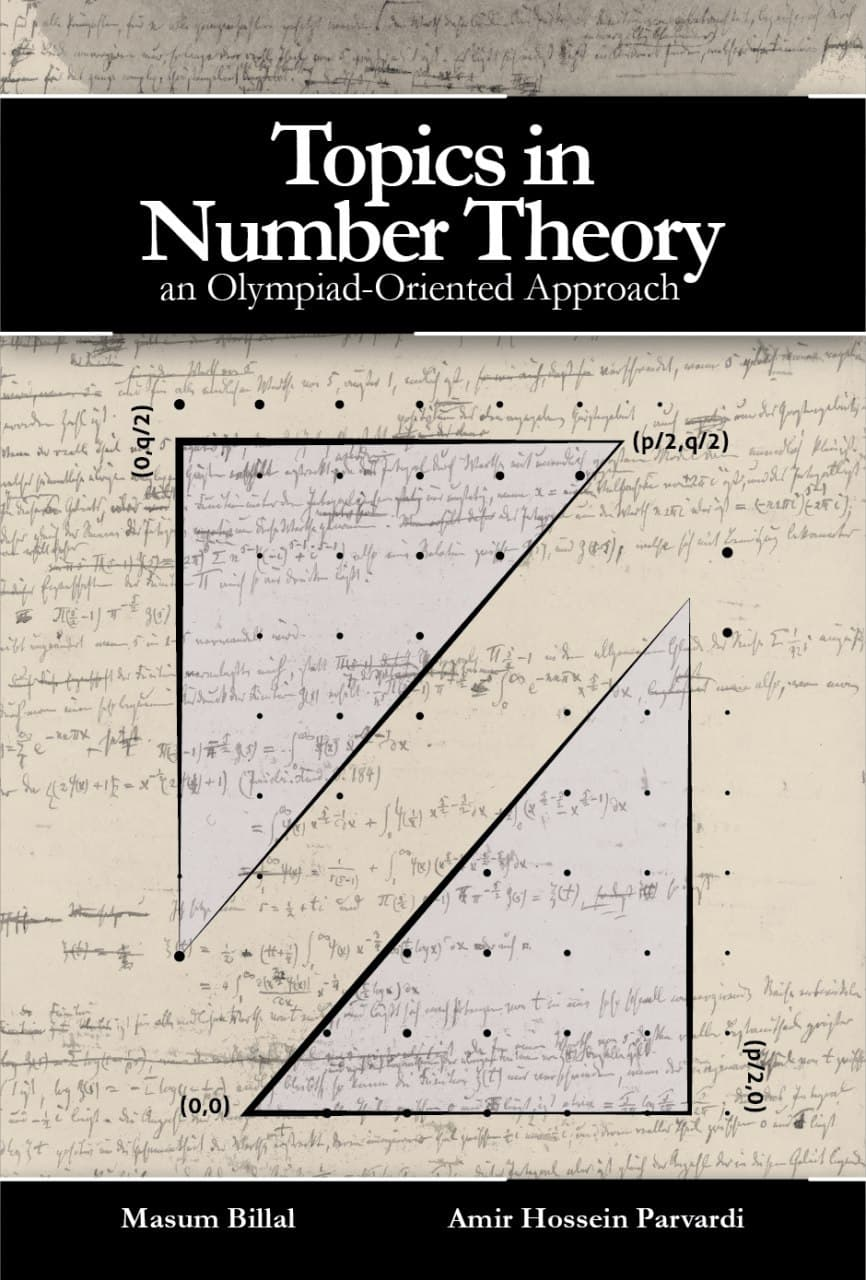
\includegraphics[origin=c,angle=0,width=\paperwidth,height=\paperheight]{TNT_Cover/FrontCover.jpg}};
\end{tikzpicture}
%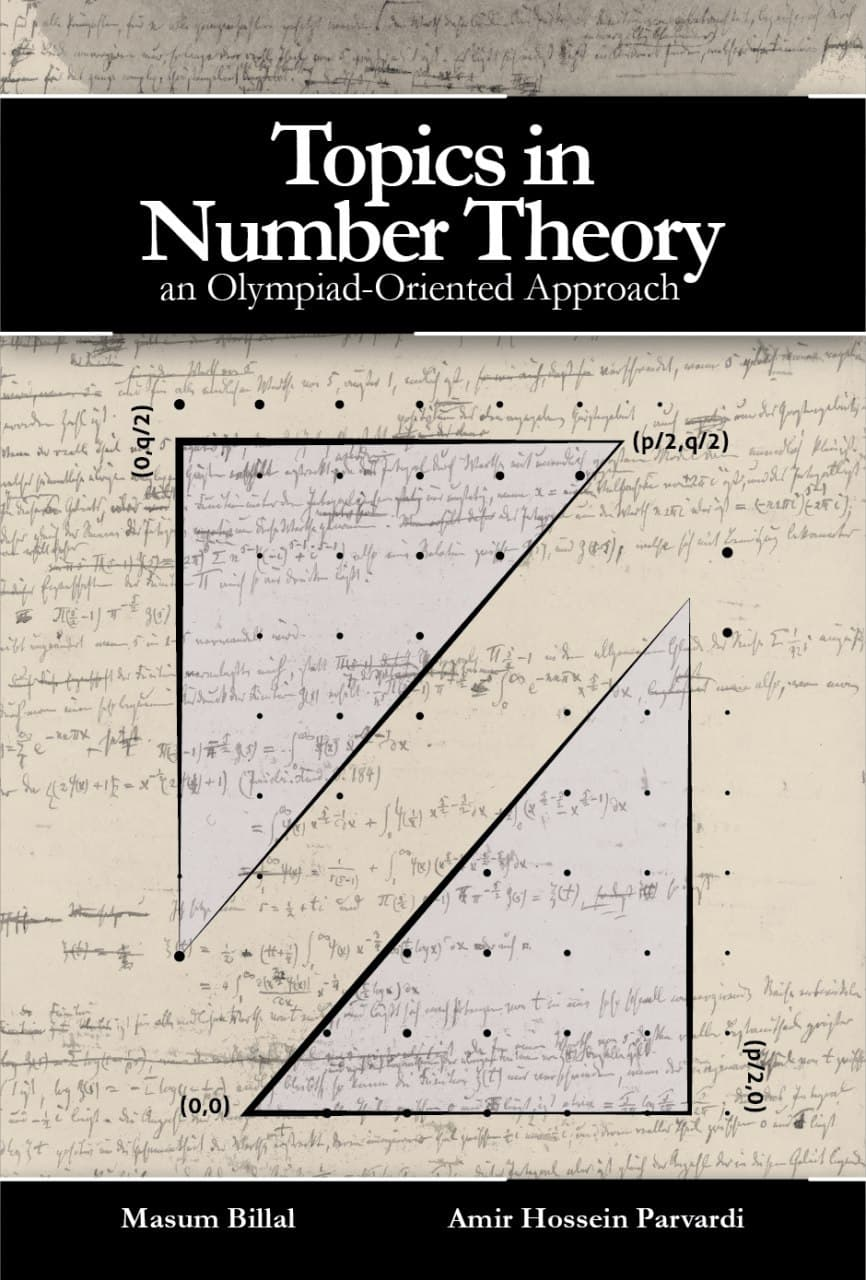
\includegraphics[width=\paperwidth,height=\paperheight]{TNT_Cover/FrontCover.jpg}
%\AddToShipoutPictureBG{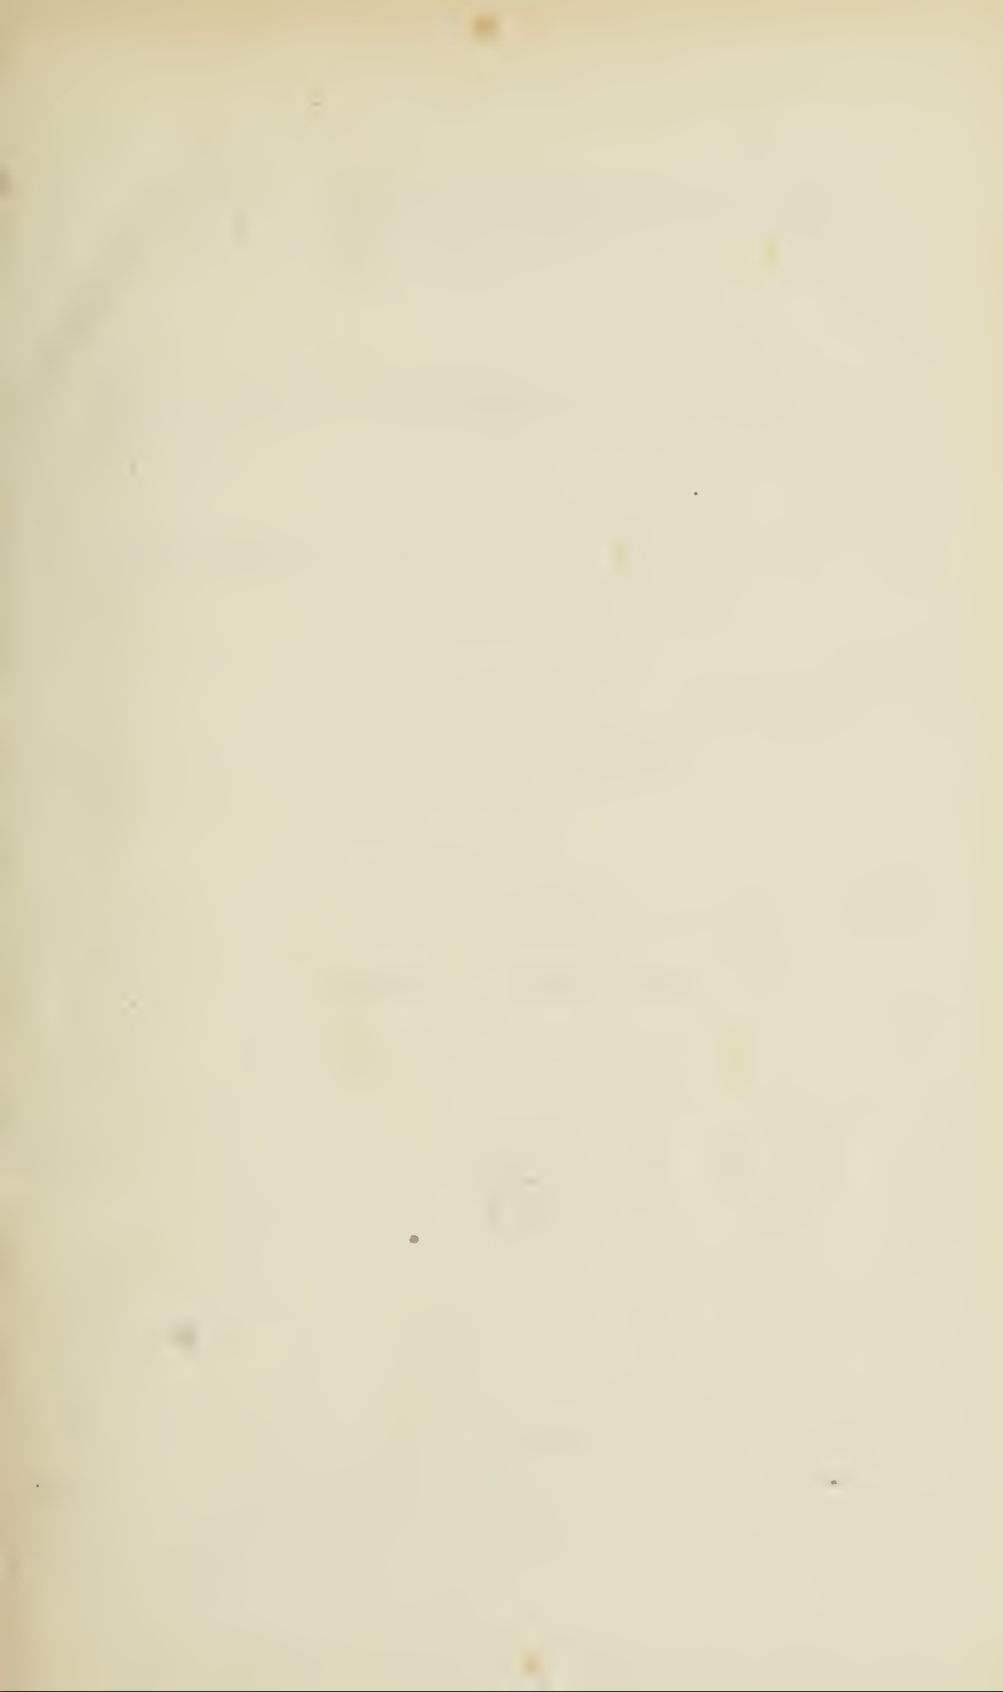
\includegraphics[width=\paperwidth,height=\paperheight]{background}}
\frontmatter
\maketitle
\pagestyle{empty}

\section*{Preface to Second Edition}
It has been over $3$ years since we have written this book. When we read the book now, we sometimes feel kind of silly. In some places, the writing comes off as childish and probably even unprofessional. But we do not regret writing the book that way. There are reasons why we have written it the way we did. We admit that we did not have the enormous amount of patience required to finish the book in a greater style. We were hurried to write a lot of the things back then. Not because we were told to, since this is an independent publication after all. There are a number of factors why we felt hurried to finish the book. For example, the book was already large even though we discarded a lot of the content we had planned for the book. In fact, we discarded most of the content we planned because the book would be so huge not even us would have been interested in reading a book that large. But that messed with our plans a lot since we had to change a lot of things on the fly. The whole reason we wanted to write a book despite there existing a lot of books on number theory is that we wanted our book to contain results or techniques that would not be as common in other Olympiad books. However, even with the minimum amount of content we decided to go with, it still felt like it was getting too large. So we tried to pick up the pace after some chapters. And one of the biggest concerns we had was that if we had not finished the book soon, we might not have been able to finish it at all. Or even worse, we could have forgotten about the whole book altogether (that has happened as well). Anyway, we mention these here not to make any excuses, nor do we feel terrible about it. Because even though the end-product does not look like the best output right now, we believe this book can still help people, at least some new students who are looking to solve number theory problems. Would the book be a lot better if we rewrote it now? Yes, probably at least ten times better. But we have neither the energy nor the time to do so. There are some updates and error fixes in this edition which hopefully improves at least some aspects of the book.

It is possible there are some \LaTeX\ issues in the new edition. If anyone finds any, please do not hesitate to email us.

\begin{flushright}
	\itshape Masum Billal\\
	Amir Parvardi\\
	August, $2021$
\end{flushright}

\newpage
\section*{Preface from first edition}

I would like to have a few words before diving into the discussion. First of all, from my personal experience, I have found that there is a common practice to learn by learning a lot of theories and then investigating how those theories are used to solve problems. As our primary audience would be students who are looking to get into mathematical Olympiads, I highly discourage this. Please do not take number theory for a collection of theories just because the word theory is literally juxtaposed with it. That being said, one could argue our book itself is a collection of a lot of theorems as well. Sadly, that is partially true for multiple reasons though it was not our intention at all.


When I first thought about writing this book, my intention was to make students realize that they do not need to know a lot of theorems in order to be able to solve problems. But as we kept writing, we had to increase the pace since we had to cover a lot (and that was discarding a lot of content which we thought would ask for even discussion or we just felt lazy about it), we had to increase the pace.


Initially, my plan was to make this book a series of $5$ volumes, this being the first one. In those volumes, I wanted to discuss a lot of topics such as special numbers like \textit{egyptian fraction} or even interesting numbers like \textit{abundant number or deficient number} and their properties, etc., or crucial topics such as \textit{Diophantine equations}. You will notice that we have left a lot of important topics like those out of this book. The reason is, I quickly realized I could hardly finish writing this first volume, and if I wanted to complete the whole series, we would probably have to keep writing my whole life. So, I had to discard a lot of content and make the book concise. This resulted in squeezing in a lot of content in a few hundred pages.


Finally, I would like to thank Amir for joining me in this project. At one point, I stopped writing the book. If he had not agreed to be a co-author, this book would have probably not been completed at all, more so because he agreed to follow the style I wanted to write in even when we had objections from a reputed publisher like \textit{Springer}.

\begin{flushright}
	\itshape Masum Billal
\end{flushright}

\newpage

In the past three years, we have always been worried about this book. It's been a long and tedious job to manage everything and edit all we had written a very long time ago. After I studied more number theory concepts of higher level, there were times that I found errors/typos in my previous drafts for the book. And that sometimes happened two or more times in a short period, and so, it was getting annoying. Anyhow, we managed to finish it at this time of the summer. It is now 5:36 AM, Tuesday, July 17, 2018, that I'm writing this. You can imagine how crazy this process has made me!

\vspace{0.3cm}
Many of our friends helped us on the way to finish this book, as mentioned in the acknowledgment, and we are so proud to have such friends. I wouldn't be able to finish my part in this book if I didn't have the support of my wonderful, beautiful, and lovely wife \textit{Nadia Ghobadipasha}. She gave me hope to choose mathematics and always believed in me. She was the only one in the hardest days of my life.
\vspace{0.3cm}
Professor \textit{Peyman Nasehpour}, whom I knew from the very first semester of my undergraduate studies in electrical engineering at the University of Tehran, helped me a lot in the process of enhancing my mathematical abilities to change my field to mathematics (number theory) for my master's.  He is an inspiration and a great colleague to me when it comes to teamwork. I'm looking forward to working with him more often.
\vspace{0.3cm}
The idea behind the lattices in the \textit{cover} is a geometric proof of the law of quadratic reciprocity. Our friends found other interpretations such as the Pick's theorem (which is not the case here) or the sum of positive integers up to $n$, which you will realize is also not always true (for all primes $p,q$). Section \eqref{sec:qrlawproof} is dedicated to this proof and investigates why it is true using counting the lattice (grid) points. When we picked this idea for the cover, we chose quadratic reciprocity because its proof is geometrically visual and indeed very beautiful. Our hope was to make the reader curious because the design looks familiar. I remember I found the idea of the proof in one of Kenneth H. Rosen's books on discrete mathematics, but I'm not sure which one, as it was a long time ago when I wrote it. I used the TikZ package for \LaTeX to write the codes and generate the graphs.
\vspace{0.3cm}
There are so many wonderful things to learn in this book. I hope you enjoy it!
\begin{flushright}
	\itshape Amir Parvardi,\\
% 	University of British Columbia,\\
	Vancouver, BC, Canada,\\
	July 2018.
\end{flushright}

\newpage

\section*{Acknowledgment}

Here is a list of all the kind people who helped us review, edit, and improve this book. The list is ordered alphabetically based on the last name.
	\begin{enumerate}
		\item Thanks to \textit{Ali Amiri}, a kind friend who helped us with the cover design.
		\item Thanks to \textit{Anr\'{e}C} from TeX.StackExchange who wrote the code for figure \eqref{fig:base16} in base conversion.
		\item We are thankful to \textit{Arta Khanalizadeh} for designing the cover of the book.
		\item Thanks to \textit{Kave Eskandari} for reading the whole book and commenting on the general points. He caught a good mistake in chapter \ref{ch:divisibility}.
		\item Cheers to our mathematical friend \textit{Leonard Mihai C. Giugiuc} from Romania that gave us positive and constructive feedback on the book. He also wrote us a wonderful review on the website.

		\item Thanks to \textit{Valentio Iverson} for proof-reading chapters \ref{ch:arithfunc} and \ref{ch:special}, and pointing out the typo in figure \eqref{fig:unitfunction}.

		\item Thanks to \textit{Aditya Khurmi} for reading the book and giving us positive feedback.

		\item We appreciate \textit{Hesam Korki}'s comments on chapter \ref{ch:divisibility}. He mentioned a few very important typos, including grammatical. He also mentioned a mathematical change of that chapter, which was very helpful.

		\item Professor \textit{Peyman Nasehpour} sent us the beautiful problem \eqref{prob:nasehpour} and an amazing solution using Prime Number Theorem. He also gave us pretty useful comments on chapter \ref{ch:divisibility}. He also introduced in section \eqref{sec:sum-of-divisors} the amicable numbers to us with a brief historical note on it.

		\item We appreciate \textit{Kenji Nakagawa}'s comments on chapters \ref{ch:primes} and \ref{ch:special}. He was one of the first people who read and reviewed these two chapters when we put them on the website of the book.

		\item We are thankful towards \textit{Mohammadamin Nejatbakhshesfahani}, Iran National Olympiad gold medalist (2010) and winner of gold medals at IMS and IMC, who honored us to read and review the whole book and gave us really instructive comments.

		\item We would like to thank \textit{Nur Muhammad Shafiullah Mahi} for his efforts to make this book better.

		\item We are honored to thank Professor \textit{Greg Martin}, a faculty member at the Mathematics Department of the University of British Columbia. He happens to be Amir Hossein's Master's supervisor. He kindly reviewed a printed draft of the book and emailed us over $10$ major points to correct in the book. We do appreciate his advice on improving the whole context of the book.

		\item We are thankful to \textit{Sohrab Mohtat} for his comments on chapter \ref{ch:divisibility}. Thanks to him, we avoided a fatal mistake at the beginning of the book. He also wrote a very useful and detailed review for our book on the website.

		\item We are thankful to \textit{Aditya Guha Roy} who reviewed the whole book and caught a few LaTeX typos, generalized lemma \eqref{lem:aditya-generalized}, fixing problems in chapter \ref{ch:unsolved}. Aditya wrote an amazing, educative review on our website.
		\item \textit{Navneel Singhal} carefully reviewed and proof-read the whole first part of the book (chapters \ref{ch:divisibility} to \ref{ch:special}) and gave us very constructive comments. We are thankful to him.

		\item Thanks to \textit{Amin Soofiani}, who is a Master's student of mathematics at the University of British Columbia, we noticed there was a mistake in theorem \eqref{thm:numofprime}. He did a perfect, precise, and detailed review on chapter \ref{ch:primes}.

		\item We are thankful to \textit{Sepehr Yadegarzadeh} for informing us about the correct \textit{umlaut}\footnote{\textit{umlaut}: a mark (\H{}), used over a vowel, as in German or Hungarian, to indicate a different vowel quality, usually fronting or rounding.} for M\"{o}bius among other grammatical and vocabulary points.
	\end{enumerate}
	%\nomenclature[c]{$\varphi(n)$}{Euler's totient function of $n$, $\varphi(n)$ is the number of positive integers not exceeding $n$ which are relatively prime to $n$.}
%\nomenclature[ca]{$J_{k}(n)$}{Jordan function of $n$, the number of tuples $(a_{1},\ldots,a_{k})$ such that $\gcd(a_{1},\ldots,a_{k},n)=1$ and $1\leq a_{1},\ldots,a_{k}\leq n$.}
\nomenclature[sets]{$\mathbb{N,N}_0$, $\mathbb{Z, Q, R, P},$ and $\mathbb{C}$}{Sets of positive integers, non-negative integers, integers, rational numbers, real numbers, primes and complex numbers respectively.}
\nomenclature[absolute]{$|a|$}{The absolute value of $a$ for any real number $a$.}
\nomenclature[divides]{$a|b$}{$b$ is divisible by $a$ without any remainder.}
\nomenclature[gcdlcm]{$\gcd(a,b)$ (for brevity, $(a,b)$) and $\lcm(a,b)$ (for brevity, $[a,b]$)}{ are greatest common divisor and least common multiple of $a$ and $b$ respectively.}
\nomenclature[coprime]{$a\perp b$}{$\gcd(a,b)=1$ or $a$ and $b$ are relatively prime.}
\nomenclature[numdiv]{$d(n)$}{Number of divisors of $n$.}
\nomenclature[totient]{$\varphi(n)$}{The number of positive integers not exceeding $n$ which are relatively prime to $n$.}
\nomenclature[numprime]{$\pi(x)$}{The number of primes not exceeding $x$.}
\nomenclature[sumdiv]{$\sigma(n)$}{Sum of divisors of $n$.}
\nomenclature[omega]{$\omega(n)$}{Number of distinct prime divisors of $n$}
\nomenclature[Omega]{$\Omega(n)$}{Number of total prime divisors of $n$}
\nomenclature[mobius]{$\mu(n)$}{M\"{o}bius function of $n$, $\mu(n)=(-1)^{\omega(n)}$ if $n$ is square-free, otherwise $\mu(n)=0$.}
\nomenclature[carmichael]{$\lambda(n)$}{Liouville function of $n$, $\lambda(n)=(-1)^{\Omega(n)}$ if $n$ is square-free, otherwise $\lambda(n)=0$. It is also used for Carmichael's universal function.}
\nomenclature[floorceil]{$\floor{x}$ and $\lceil x \rceil$}{The largest integer not greater than $x$ and the smallest integer integer not less than $x$ respectively.}
\nomenclature[legendre]{$\parenthesis{\dfrac{a}{p}}$}{The Legendre symbol for an integer $a$ and prime $p$.}
\nomenclature[jacobi]{$\parenthesis{\dfrac{a}{n}}$}{The Jacobi symbol for an integer $a$ and a positive integer $n$.}
\nomenclature[binom]{$\binom{n}{k}$}{$n$ choose $k$, the binomial coefficient of the $k+1$-th term in the expansion of $(1+x)^{n}$.}
\nomenclature[nu]{$v_n(a)$}{Largest non-negative integer $\alpha$ so that $n^\alpha|a$ but $n^{\alpha+1}\nmid a$.}
\nomenclature[mangoldt]{$\Lambda(n)$}{Von Mangoldt Function of $n$. $\Lambda(n)=\log{p}$ if $n=p^{e}$ for some positive integer $e$, otherwise $\Lambda(n)=0$.}
\nomenclature[theta]{$\vartheta(x)$}{Tchebycheff function of the first kind.}
\nomenclature[psi]{$\psi(x)$}{Tchebycheff function of the second kind.}
\nomenclature[zeta]{$\zeta(s)$}{Zeta function of the complex number $s$.}
\nomenclature[dirconv]{$\alpha\ast\beta$}{Dirichlet convolution of two arithmetic functions $\alpha$ and $\beta$.}
\nomenclature[genconv]{$\alpha\circ\beta$}{General convolution of two arithmetic functions $\alpha$ and $\beta$.}
%\nomenclature[gamma]{$\gamma$}{Euler-Mascheroni constant.}
\nomenclature[rad]{$\rad(n)$}{Product of distinct prime divisors of $n$, $\rad(n)=\prod_{p\mid n}p$.}

	\printnomenclature
	\tableofcontents
	\mainmatter
	\pagestyle{headings}
	\documentclass{subfile}

\begin{document}
	\part{Fundamentals}
	\chapter{Divisibility}\label{ch:divisibility}

	\section{Definitions and Propositions}
	Let us start from the very basics. Whenever you encounter a definition, try to make sense of it with a few examples. As we move on to next sections, you will get used to the divisibility terms and notation. The following definitions are designed to teach a beginner student the basics of divisibility, so please do not bore yourself with them\watermark.
	\begin{definition}\label{def:remainder}
		When an integer $b$ is divided by another (non-zero) integer $a$, we can write $b=aq+r$ for some integers $q$ and $r$. In this most general case, we call $r$ the \textit{remainder} of the division.

		However, if we choose $q$ such that $0\leq r< |a|$, then we say $r$ is the \textit{minimum remainder} of the division\footnote{$|x|$ is the absolute value of $x$.}.

		At times, it is convenient to carry out the division (i.e., choose $q$) so that $b$ is as close as possible to an integral multiple of $a$. Then we can write $b = aq + r$, with $|r| \leq |a/2|$ for some integer $q$.  In this case, we call $r$ the \textit{minimum absolute remainder}.
	\end{definition}

	\begin{note}[1]
		We will prove later that the minimum remainder is unique. That is, there exists exactly one value for $r$ such that $b=aq+r$ and $0 \leq r <a$. Because of its uniqueness and non-negativity, remainder in this book will mean minimum remainder unless otherwise stated.
	\end{note}

	\begin{note}[2]
		When we talk about the the minimum absolute remainder in the division $b=aq+r$, note that if $a$ is odd, we will have a unique $r$. That is, there exist only one possible value for $r$ such that $|r| \leq \left|a/2\right|$. However, if $a$ and $b$ both are even, there can be two possible values for $r$. For example, if $a=20$ and $b=8$, the division can be done as both $20=8\cdot2+4$ and $20=3\cdot8-4$ and we would have two values for $r$: $4$ and $-4$. To force $r$ to be unique in this case, we will take the positive value of $r$ as the minimum absolute remainder. Therefore, in our example, $20=2\cdot8+4$ would be accepted as the division equation and $r=4$ is the minimum absolute remainder.
	\end{note}

% Fixed it:
% In the next definition, we have swapped $a$ and $b$ and written $b=aq+r$ instead of $a=bq+r$.

	\begin{definition}
		If $b=aq+r$ is the proper division of $b$ by $a$ (that is, a division in which $r$ is the minimum remainder), $b$ is the \textit{dividend}, $a$ is the \textit{divisor}, and $q$ is the \textit{quotient}.
	\end{definition}

	\begin{example}
		Let $b=23$ and $a=5$. The division of $b$ by $a$ can be done in many ways. Take $23=5\cdot2+13$, so we can say $13$ is a remainder of $23$ upon division by $5$, but not a minimum remainder. If we write the division as $23=5\cdot4+3$, then $3$ is the minimum remainder. And if we write it as $23=5\cdot5+(-2)$, then $-2$ is the minimum absolute remainder.
	\end{example}

	If we divide $4$ by $2$, we get a zero remainder. In this case, we say that $4$ is \textit{divisible} by $2$ and write it as $2\mid 4$.

	\begin{definition}
		Let $a$ and $b$ be two integers. If $b$ leaves a zero remainder upon division by $a$, or equivalently, if there is an integer $k$ for which $b=ak$, we write $a \mid b$ and say that
		\begin{itemize}
			\item $b$ is \textit{divisible} by $a$,
			\item $a$ \textit{divides} $b$,
			\item $a$ is a \textit{divisor} (or a \textit{factor}) of $b$, or
			\item $b$ is a \textit{multiple} of $a$.
		\end{itemize}
		Likewise, $a\nmid b$ denotes that $b$ is not divisible by $a$.
	\end{definition}

	\begin{remark}
		Some (Eastern) authors use the notation $b\vdots a$ instead of $a\mid b$, but it is not as common.
	\end{remark}

	\begin{definition}
		If $a$ divides $b$ and $|a|<|b|$, the number $a$ is called a \textit{proper divisor} of $b$. Here, $|a|$ denotes the absolute value of $a$. For example, $|-5|=5$ and $|5|=5$.
	\end{definition}

	\begin{example}
		$4 \mid 20$ and $5 \mid 20$ but $11\nmid\mid 20$.
	\end{example}

	\begin{example}
		$1$ is a divisor of all integers.
	\end{example}

	You can also try to make sense of division in this way: $8$ divides $40$ because $40$ has every factor that $8$ has in it. In other words, if $8$ had a factor which was not a factor of $40$, then $40$ would not be divisible by $8$. For example, $42$ does not have the factor $4$, which is a factor of $8$, therefore $8 \nmid\mid 42$.

	\begin{definition}[Prime and Composite Numbers]
		An integer $n>1$ is called \textit{prime} if it has exactly two distinct (positive) divisors, namely $1$ and $n$ itself. A number greater than $1$ which is not a prime is \textit{composite}. In other words, an integer $n$ is composite if it has a proper divisor other than $1$. We do not wish to discuss primality for negative integers.
	\end{definition}

	\begin{note}
		When we say $a$ is a divisor of $b$, unless otherwise stated, we usually mean $a$ is a \textit{positive} divisor of $b$. This is distinguished because negative divisors exist as well.
	\end{note}

	\begin{question}
		Is $1$ a prime number? If so, why? If not, how is it a composite number? You may be already familiar with prime numbers and in that case, the definition you know may seem a little different. Try to understand why we chose to stick with the above definition of primes rather than the following: \textit{a positive integer $n$ that is not divisible by any positive integer other than $1$ and $n$ is a prime}.
	\end{question}

	\begin{definition}[Parity]
		Parity is the property of an integer being \textit{even} or \textit{odd}. An even number is one which is divisible by $2$. Odd numbers, on the other hand, leave a remainder of $1$ when divided by $2$.
	\end{definition}

	\begin{example}
		$2$ and $4$ have the same parity; they are both even. $5$ and $10$ are of different parity; $5$ is odd and $10$ is even.
	\end{example}

	\begin{example}
		$11$ is a prime because no positive integer greater than $1$ and less than $11$ divides it. Similarly $2,3,$ and $29$ are primes, but $169$ (divisible by $13$) and $1001$ (why?) are composites. If a number is divisible by $2$, it is composite. Thus, the only even prime is $2$.
	\end{example}

	If we add or subtract two numbers of the same parity, the answer will be even. Conversely, the result of addition or subtraction of two numbers with different parities is always an odd number. Using these two facts, you can easily find many properties of integers related to parity. For instance, we can say that if we add or subtract an even number to or from a positive integer $n$, the parity does not change; i.e., parity remains {\it invariant} in this case. Moreover, any odd multiple of $n$ has the same parity as $n$.

	We usually deal only with positive integers in divisibility relations. However, sometimes negative integers or zero also come into play.

	\begin{proposition}[Basic Properties of Divisibility]\label{prop:basicdiv}
		For any three integers $a,b$, and $c$, the following statements are true.
		\begin{enumerate}
			\item $a\mid 0$.
			\item $a\mid a$.
			\item $1\mid a$ and $-1\mid a$.
			\item If $a$ is non-zero, then $0 \nmid\mid a$.\footnote{Does zero divide zero? That depends on the context. In arithmetic, we can write $0 = 0\cdot 0 + 0$, so technically $0 \mid 0$ in number theory. However, when studying real analysis, division is defined as multiplying by the multiplicative inverse, which means that $0/0$ is undefined and therefore, $0 \nmid \mid 0$ with that logic.}
			\item If $a \mid b$, then $a\mid -b$, $-a\mid b$, and $-a\mid -b$.
			\item If $a\mid b$, then $a\mid bk$ for all integers $k$.
			\item If $a\mid b$, then $ak\mid bk$ for all integers $k$.
			\item If $ak\mid bk$ for some non-zero integer $k$, then $a\mid b$.
			\item If $a\mid b$ and $b\mid c$, then $a\mid c$. \footnote{\textit{Keith Conrad} states this as a mantra: ``A factor of a factor is a factor.''}
			\item If $a\mid b$ and $b\neq 0$, then $|b| \geq |a|$. Consequently, if $a\mid b$ and $|a|>|b|$, then $b=0$.
			\item If $a\mid b$, then $a^n\mid b^n$ for all non-negative integers $n$.
			\item If $a^n \mid b^n$ for some positive integer $n$, then $a\mid b$.
		\end{enumerate}

	\end{proposition}

	\begin{proof}
		Most of the parts are trivial and we prove only the important ones. A general approach to solve this kind of problems is simply transforming them into equations. That is, when $x\mid y$, write $y=kx$ for some integer $k$.
		\begin{enumerate}
			\setcounter{enumi}{3}
			\item Assume that $0\mid a$ for some integer $a$. This means that $a=0k$ for some integer $k$. Therefore, $a=0$ is the only integer that is divisible by zero (in number theory).
			\setcounter{enumi}{5}
			\item $a\mid b$ means that $b=aq$ for some $q$. Multiply both sides of this equation by $k$ to get $bk = akq=aq'$. Therefore $a\mid bk$.
			\setcounter{enumi}{8}
			\item $a\mid b$ and $b\mid c$, so $b=aq_1$ and $c=bq_2$ for some integers $q_1$ and $q_2$. Combine these two equations to get $c = aq_1q_2 = aq$, thus $a\mid c$.
			\setcounter{enumi}{9}
			\item $a\mid b$, so $b = ak$ for some integer $k$. Rewrite this equation in absolute value terms: $|b| = |ak| = |a| \cdot |k|$. Since $k$ is a non-zero integer, the smallest value for $|k|$ is $1$, so $|b| = |a| \cdot |k| \geq |a|$.
			\setcounter{enumi}{11}
		\end{enumerate}
	\end{proof}

	\begin{note}
	    You may think that it is straightforward to prove statement $(12)$ in the above Proposition. However, it is not so simple. The reason is we need to prove that if $$\frac{b^n}{a^n}=\left(\frac{b}{a}\right)^n$$ is an integer, then so is $\frac{b}{a}$. This is not obvious (try to make sense why).
	\end{note}

	\begin{proposition}\label{prop:bothdivide}
		If $a \mid b$ and $b \mid a$, then  $|a|=|b|$. In other words, $a=\pm b$.
	\end{proposition}

	\begin{proof}
		The proof is quite simple using part $10$ of the previous proposition. In fact, we get $|b| \geq |a|$ and $|a| \geq |b|$, which means $|a| = |b|$ or $a = \pm b$.
	\end{proof}
	The above proposition often comes handy when you want to prove that two expressions are equal. If you can show that each expressions divides the other one and that they have the same sign (both positive or both negative), you can imply that their values are equal.

	\begin{proposition}
		For fixed positive integers $a$ and $b$, there are unique integers $q$ and $r$ so that $b=aq+r$ with $0\leq r<a$. In other words, the quotient and the minimum remainder of the division are unique.
	\end{proposition}

	\begin{proof}
		We can easily rule out the case $r=0$. Just notice that $a\mid b$.

		We can now assume that $a\nmid b$. Then, $b$ must have a nonzero remainder upon division by $a$, say $r$. One can rewrite the equation $b=aq+r$ as $aq=b-r$ or $q=(b-r)/a$. This simply means that uniqueness of $r$ implies the uniqueness of $q$. Therefore, we only need to prove that $r$ is unique. Assume that there exist integers $q'$ and $r'$ so that
		\begin{align*}
			b
				& =aq+r\\
				& =aq'+r'
		\end{align*}
		This implies $a(q-q')=r'-r$, which shows that $r'-r$ is divisible by $a$. Is it possible? The answer is clearly no. Since $r'$ and $r$ are both less than $a$, we have $|r'-r|<a$. By part $10$ of proposition \eqref{prop:basicdiv}, we must have $|r'-r|=0$, which gives $r'=r$. This means two remainders are the same and the minimum remainder is unique. The proof is complete.
	\end{proof}

	%	\begin{corollary}
	%		If $b$ leaves a remainder of $r$ when divided by $a$, then we can write $b=aq+r$ for some integer $q$.
	%	\end{corollary}

	\begin{question}
		We know that $4\mid 20$ and $4\mid 16$. Do they imply $4\mid 20+16$? Again, this is not too obvious. Try to prove it first.
	\end{question}

	\begin{proposition}\label{prop:a|bx+cy}
		If $a\mid b$ and $a\mid c$, then $a\mid bx+cy$ for any arbitrary integers $x$ and $y$. In particular, we have $a\mid b\pm ak,a\mid b+c$, and $a\mid b-c$.
	\end{proposition}

	\begin{proof}
		Since $a\mid b$, there is an integer $k$ so that $b=ak$. Similarly, there is an integer $\ell$ so that $c=a\ell$. Therefore,
		\begin{align*}
			bx+cy
				& =akx+a\ell y\\
				& =a(kx+\ell y)
		\end{align*}
		which is certainly divisible by $a$ since it has a factor $a$ in it.
	\end{proof}

	\begin{note}
		Here, $x$ and $y$ can be negative integers as well. This shows how negative numbers may come into play even when we start off with positive integers.
	\end{note}

	\begin{question}
		Let $a,b$, and $n$ be positive integers such that $a\mid n$ and $b\mid n$. Do we have $ab \mid n$?
	\end{question}
	This is a very common mistake among new problem solvers. Consider an integer that is divisible by both $6$ and $4$. Is that integer divisible by $4\cdot6=24$? If you think the answer is yes, think again! How about $12$?

	In general, the answer is a big NO. Try to find a few more counterexamples and then find the condition when we can be certain that $ab \mid n$ if $a\mid n$ and $b\mid n$. We will now focus on prime divisors.

	\begin{proposition}
		Any integer $n$ greater than $1$ has a prime divisor.
	\end{proposition}

	\begin{proof}
		If $n$ itself is a prime, we are done. So, assume $n$ is composite. By definition, $n$ has a proper divisor, i.e., there is an integer greater than $1$ and less than $n$ which divides $n$. Call this divisor $d$. Now, if $d$ is not a prime, then $d$ has a divisor too. We can continue like this until we reach a point where $d$ does not have a proper divisor greater than $1$. We know by definition that only a prime number does not have a proper divisor other than $1$. Therefore, that divisor must be a prime.
	\end{proof}

	\begin{corollary}\label{cor:smallestdivisor}
		Let $n$ be a positive integer larger than $1$. The smallest divisor of $n$ is a prime.
	\end{corollary}

	You should be able to prove the following proposition by yourself. Even if you can not prove it formally, at least make sense of why this is true. We will not prove it here. Try not to skip it and move on. Can you use induction\footnote{The traditional induction process. Prove the claim for a base case, say $n_0$. Assume the claim is true for $n=m$, then prove it for $n=m+1$.} to prove it? How about using the facts you already know?

	\begin{proposition}[Euclid's Lemma]\label{prop:euclidslemma}
		Let $a$ and $b$ be two integers. If $p$ is a prime and $p\mid ab$, then either $p\mid a$ or $p\mid b$.
	\end{proposition}

	\begin{corollary}\label{cor:euclidgeneral}
		If a prime divides the product of some integers, it divides at least one of them.
	\end{corollary}

	\begin{proposition}\label{factorsqrt}
		Every composite $n$ has a prime factor less than or equal to $\sqrt{n}$.
	\end{proposition}

	\begin{proof}
		Since $n$ is composite, it has at least one proper prime divisor. {\it Consider the smallest prime factor $p$ of $n$} and write $n=pk$ for some integer $k$. Of course $p\leq k$, because otherwise according to Corollary \eqref{cor:smallestdivisor}, the smallest prime factor would be $k$ or one of its divisors. Therefore,
		\begin{align*}
			n=pk\geq p^2
		\end{align*}
		which in turn implies $p\leq \sqrt{n}$.
	\end{proof}

	This proposition is quite useful to test the primality of a number. It implies that it suffices to check if $n$ is divisible by any of the primes less than or equal to $\sqrt{n}$. If it is, then $n$ is not a prime. Check this with some simulations by hand, say for $11,25,$ and $479$. However, the test can be quite lengthy and tedious if $n$ is too large and its smallest prime factor is not small. If you are curious how lengthy this test can be, take the number $357 \ 879 \ 581$ and try finding its smallest prime divisor.

	\begin{definition}[Prime Factorization]
		Prime factorization is the process of finding all the prime factors of a positive integer.
	\end{definition}

	The fact that every positive integer greater than $1$ has a prime factorization gives birth to the \textit{Fundamental Theorem of Arithmetic}.

	\begin{theorem}[Fundamental Theorem of Arithmetic]
		Every positive integer $n$ larger than $1$ can be written as a product of primes \textit{in a unique way}. We write this factorization as
		\begin{equation}
			n=p_1^{e_1}p_2^{e_2}\cdots p_k^{e_k}\label{eqn:one}
		\end{equation}
		where $p_1,p_2,\cdots p_k$ are different primes and $e_1,e_2,\cdots e_k$ are positive integers. Using product notation, we can write equation \eqref{eqn:one} as
		\begin{align*}
			n
				&=\prod\limits_{i=1}^{k}p_i^{e_i}\\
				& =\prod\limits_{p\mid n}p^e
		\end{align*}
		In the second product notation above, $p$ runs through all primes dividing $n$ and $e$ is the maximum power of $p$ that divides $n$.\footnote{Make sure you understand the notations $\sum$ and $\prod$.}
	\end{theorem}

	\begin{proof}
		We first prove by induction that the factorization indeed exists. Suppose that all numbers $k$ such that $1<k<n$ have a factorization. If $n$ is a prime, its factorization is obvious. Otherwise, there exist positive integers $a$ and $b$ both less than $n$ such that $ab=n$. By induction hypothesis, $a$ and $b$ both have factorizations. Let $a=p_1^{\alpha_1}p_2^{\alpha_2}\cdots p_k^{\alpha_k}$ and $b=q_1^{\beta_1}q_2^{\beta_2}\cdots q_l^{\beta_l}$ be the prime factorizations of $a$ and $b$. Then,
		\begin{align*}
			n
				& = ab\\
				& = p_1^{\alpha_1}p_2^{\alpha_2}\cdots p_k^{\alpha_k}q_1^{\beta_1}q_2^{\beta_2}\cdots q_l^{\beta_l}
		\end{align*}
		This is a prime factorization for $n$ and the induction is complete.

		Now, let us prove that the prime factorization of $n$ is unique. Suppose that there are two factorizations for $n$. That is,
		\begin{align}
			p_1^{\alpha_1}p_2^{\alpha_2}\cdots p_s^{\alpha_s}
				& =q_1^{\beta_1}q_2^{\beta_2}\cdots q_t^{\beta_t} \label{eq:fundamentalarith-eq1}
		\end{align}
		are two factorization of $n$, where $p_i$ and $q_j$ are primes and $\alpha_i$ and $\beta_j$ are positive integers ($1 \leq i \leq s, 1 \leq j \leq t$). The above equation implies that $p_1$ divides $q_1^{\beta_1}q_2^{\beta_2}\cdots q_t^{\beta_t}$. By generalization of Euclid's lemma (Corollary \eqref{cor:euclidgeneral}), $p_1$ must divide at least one of $q_1^{\beta_1},q_2^{\beta_2},\dots,$ or $q_t^{\beta_t}$. Without loss of generality, suppose that $p_1\mid q_1^{\beta_1}$. Since $q_1$ is a prime, the only prime divisor of $q_1^{\beta_1}$ is $q_1$. This means that $p_1=q_1$ and $\alpha_1=\beta_1$. Divide both sides of equation \eqref{eq:fundamentalarith-eq1} by $p_1$ to obtain
		\begin{align*}
			p_2^{\alpha_2}p_3^{\alpha_3}\cdots p_s^{\alpha_s}
				& =q_2^{\beta_2}q_3^{\beta_3}\cdots q_t^{\beta_t}
		\end{align*}
		With similar reasoning, we can deduce that $p_2^{\alpha_2}$ is equal to some other $q_j^{\beta_j}$, say $q_{2}^{\beta_2}$. Continuing this process, one soon realizes that $t=s$ and all prime powers in the left side of equation \eqref{eq:fundamentalarith-eq1} appear in the right side, but maybe in a different order. In other words, the two factorizations of $n$ are the same and the uniqueness of factorization is implied.
	\end{proof}

	\begin{example}
		Try to understand the following examples and match them with the factorization formula:
		\begin{itemize}
			\item $12=2^2\cdot3$. Here, $p_1=2,e_1=2,p_2=3,e_2=1$
			\item $180=2^2\cdot 3^2\cdot 5$. So,  $p_1=2,e_1=2,p_2=3,e_2=2,p_3=5,e_3=1$
		\end{itemize}
		The factorization of $n$ is unique no matter in what order you factor out the primes. Also, note that all the powers are positive. We could bring primes with power zero but that does not make any sense (because any number to the power of zero yields $1$ and the product would not be changed).
	\end{example}

	\begin{note}
		In the product $n=\prod\limits_{i=1}^{k}p_i^{e_i}$, $k$ is the number of distinct prime factors of $n$. For example, if $n=12$, then $k=2$ since $12$ has only two distinct prime factors: $2$ and $3$. If $n=180$, then $k=3$ because $2,3,$ and $5$ are the only prime factors of $n$.
	\end{note}

	As explained above, one way to factorize a number $n$ is to divide it by all primes less than $\sqrt n$. Dividing a number by another would be pretty boring for large numbers. In order to simplify the process, next section provides some rules for divisibility by some specific numbers like $3, 5, 7, 11$, etc.

\subsection{Divisibility by Certain Numbers}\label{subs:divrules}

As soon as one is introduced to the concept of natural numbers, one can make sense of odd and even numbers. We all know that an even number, namely a number that is divisible by $2$, must have an even rightmost digit (ones digit). We also know the \textit{rules of divisibility} for $5$: a number is divisible by $5$ if and only if its ones digit is. Let us make our knowledge concrete and write a proof for these two simple facts.

	\begin{proposition}[Divisibility by $2$]
		A number is divisible by $2$ if and only if its last digit is even (one of $0,2,4,6,8$).
	\end{proposition}

	\begin{proof}
		Suppose that one has the number $x = \overline{x_{k-1}x_{k-2} \ldots x_0}$, where $x_i$ ($0 \leq i \leq k-1$) are its digits (so the number has $k$ digits). One can write
			\begin{align*}
				x
					&= \overline{x_{k-1} x_{k-2} \ldots x_1 0} + x_0\\
					& = 10 \cdot \overline{x_{k-1} x_{k-2} \ldots x_1} + x_0
			\end{align*}
		It is now clear that the first term in the right-hand side of the latest equation is divisible by $2$ (because $2 \mid 10$). So, $x$ is divisible by $2$ if and only if $x_0$ is even.
	\end{proof}

The proof of the rule of divisibility by $5$ is very similar and left as an exercise for the reader.

	\begin{proposition}[Divisibility by $5$]
		A number is divisible by $5$ if and only if it has $0$ or $5$ as last digit.
	\end{proposition}

So far, we discovered and proved the rules of divisibility by $2$ and $5$. Is it always possible to find a divisibility rule for division by a given arbitrary number $n$? Maybe the question is somehow unclear at the moment. We need to define a \textit{divisibility rule} first:

	\begin{definition}
		Let $n>1$ be any integer. A divisibility rule for $n$ is defined to be a process which leads to determining whether a given natural number is divisible by $n$.
	\end{definition}

Let's think about the question again. Can we find a divisibility rule for any $n>1$? The answer is obviously yes. With our definition of a divisibility rule, you can consider division by $n$ as a divisibility rule. One can always divide a natural number by $n$ and find the remainder of the division. The number is divisible by $n$ if and only if this remainder is equal to zero.

Well, of course, that is not what we had in mind. We are looking for divisibility rules that make our life simpler, not the ones which ask you to do it by brute force. So, it would be wise to refine our definition:

	\begin{definition}
		Let $n>1$ be any integer. A \textit{proper} divisibility rule for $n$ is a divisibility rule which uses a recursive algorithm. From now on, by a divisibility rule, we mean a proper one.
	\end{definition}

As an example, recall the rule of divisibility by $3$. To find out the remainder of a number upon division by $3$, we add up all the digits to create a smaller number. This is the \textit{recursive} step: we are doing a simple process (adding the digits) to transform our initial given number (which we suppose is large) into a new number which is smaller in size. Then, we find the remainder of the new smaller number by $3$. We know from high school (or elementary school) that the remainder of the new number when divided by $3$ is the same as that of the original number.

In general, we are looking for divisibility rules which explain a method for creating a smaller number from an initially large given number. This new number has one thing in common property with the initial number: its remainder when dived by $n$. We can repeat this algorithm as many times as we wish until we reach numbers small enough for us to do the division by hand. We know that our iterative algorithm will terminate at some point because you cannot go smaller than $1$.

It is quite easy to see that the algorithm for checking divisibility by $3$ is indeed very fast and terminates quickly. That is, the algorithm is \textit{time-efficient}. Suppose that you have a $100$ digit number and you want to check its divisibility by $3$. Dividing the number by $3$ to find the remainder is the worst thing to do because there is probably no calculator which can do this task for you and you would need to do the division by hand. Now, if you use the algorithm provided above, you would need to sum up all the digits of the number, which would be at most $100 \times 9 = 900$ (in case where all the digits are the largest, $9$), and then find the remainder of this sum upon division by $3$. If you are reading this text right now, you must be able to divide any three digit number by $3$ without using a calculator. So, this algorithm terminates after one iteration in this case because you will find the remainder right after finding the sum of the digits. Considering we started with a $100$ digit number, that is assumed to be a pretty fast algorithm.

Let's see the mathematical idea behind the divisibility rule for $3$.


	\begin{proposition}[Divisibility by $3$]
		A number is divisible by $3$ if and only if the sum of digits of the number is divisible by $3$.
	\end{proposition}

	\begin{example}
		Take the number $951$ which has a sum of digits $9+5+1=15$, divisible by $3$. According to our claim, $951$ should be divisible by $3$ and indeed it is: $951=3\cdot317$.
	\end{example}

	\begin{proof}
		The secret lies behind the fact that $10 = 3 \cdot 3 + 1$. Write your initial number $x = \overline{x_{k-1} x_{k-2}\ldots x_0}$ as
			\begin{align*}
				x & = 10^{k-1}x_{k-1} + 10^{k-2}x_{k-2} + \cdots + 10x_1 + x_0\\
				&= (3 \cdot 3 + 1)^{k-1}x_{k-1} + (3 \cdot 3 + 1)^{k-2}x_{k-2} + \cdots + (3 \cdot 3 + 1)x_1 + x_0
			\end{align*}
		Try to show as an exercise that the remainder of division of $(3 \cdot 3 + 1)^{i}$ (for $1 \leq i \leq k-1$) is always equal to $1$ (hint: you might want to use theorem \gls{binomial}). In other words, there exist integers $q_i$ (for $1 \leq i \leq k-1$) such that $(3 \cdot 3 + 1)^{i} = 3q_i + 1$. Therefore,
			\begin{align*}
				x &= (3 \cdot 3 + 1)^{k-1}x_{k-1} + (3 \cdot 3 + 1)^{k-2}x_{k-2} + \cdots + (3 \cdot 3 + 1)x_1 + x_0\\
				&= (3q_{k-1}+1)x_{k-1} + (3q_{k-2}+1)x_{k-2} + \cdots  + (3q_{1}+1)x_{1} + x_{0}\\
				&= 3(q_{k-1} + q_{k-2} + \cdots + q_1)  + x_{k-1} + x_{k-2} + \cdots + x_1 + x_0
			\end{align*}
		It is now clear that $3(q_{k-1} + q_{k-2} + \cdots + q_1)$ is always divisible by $3$. This means that the remainder of $x$ upon division by $3$ is the same as that of $x_{k-1} + x_{k-2} + \cdots + x_1 + x_0$, which is the sum of digits of $x$. It remains to verify the other direction, but all we did can be reversed and so the other direction also follows. The proof is complete.
	\end{proof}

You might be curious if we can find such simple proper divisibility rules for other numbers. Unfortunately, the recursive algorithms we find for (most of) other numbers are not always time-efficient like that of $3$ and it is possible that we need to wait for several iterations for the algorithm to terminate.

Another issue that we need to discuss is the following: for which numbers $n$ do we really need a divisibility rule? For instance, now that we know the divisibility rules for $2$ and $3$, do we really need another rule for divisibility by $6$? No! We know that a number is divisible by $6$ if and only if it is divisible by both $2$ and $3$. If the previous sentence is not clear for you, think about it for a few minutes and investigate some examples to see why it is true. You don't need to know a rigorous proof of this fact; just convince yourself that it is true.


\begin{proposition}[Divisibility by $6$]
	A number is divisible by $6$ if and only if it is even and divisible by $3$.
\end{proposition}

We got that there is no need for us to define a divisibility rule for $6$ because we already know rules for $2$ and $3$. There is nothing special about $6=2 \cdot 3$. In general, we do not need a divisibility rule for $pq$, where $p$ and $q$ are distinct primes, if we already have rules for $p$ and $q$.

\begin{proposition}[Divisibility by $pq$] \label{prop:divisibility-pq}
	Let $p$ and $q$ be distinct primes. A number is divisible by $pq$ if and only if it is divisible by both $p$ and $q$.
\end{proposition}

\begin{proof}
	The only if part is pretty obvious: if $n$ is divisible by $pq$, then it is divisible by both $p$ and $q$. To prove the if part, assume that a positive integer $n$ is divisible by both $p$ and $q$. From divisibility by $p$, we can write $n=pk$ for some integer $k$. Since $p$ and $q$ are different, $p$ is not divisible by $q$. Since $n=pk$ is divisible by $q$, we must have that $q$ divides $k$. This means that $k=ql$ for an integer $l$. Finally, $n=pql$, which implies that $n$ is divisible by $pq$.
\end{proof}


You have probably figured out where this is going: we only need divisibility rules for $n$ when $n$ is either a prime or a power of a prime. The other cases would follow from the next corollary of proposition \eqref{prop:divisibility-pq} (can you explain why?).

\begin{corollary}
	Let $m$ and $n$ be two positive integers (not necessarily primes) which do not share any common divisors. Then, a number is divisible by $mn$ if and only if it is divisible by both $m$ and $n$.
\end{corollary}

We said that in order to find divisibility rules for all natural numbers, we need a divisibility rule for primes as well as their powers. Finding divisibility rules for powers of primes other than $2$, $3$, and $5$ would not be something of interest for our book. We will discuss only divisibility rules for powers of $2$. Let's see the most basic case, $4=2^2$.

\begin{proposition}[Divisibility by $4$]
	A number is divisible by $4$ if and only if the number formed by its last two digits is divisible by $4$.
\end{proposition}

\begin{example}
	$202\, 390\, 2348$ has the last two digits $4$ and $8$ which make the number formed by its last two digits $48$. Since $48$ is divisible by $4$, the number $202\, 390\, 2348$ is divisible by $4$.
\end{example}

What about $2^3=8$?

\begin{proposition}[Divisibility by $8$]
	A number is divisible by $8$ if and only if the number formed by its last three digits is divisible by $8$.
\end{proposition}

If you have a curious mind, you should already notice a pattern in the divisibility rules for $2,4$, and $8$. For $2$, we only check the last digit. For $4$, we check the last two digits and for $8$, the last three digits. Do you see the pattern now? $2=2^1,4=2^2$ and $8=2^3$. You can easily check that the same is true if we take $16=2^4$. To check divisibility by $16$, it suffices to test the number formed by the last $4$ digits. We can generalize this result for $2^k$.

\begin{theorem}[Divisibility by $2^k$]
	Let $k$ be a positive integer. A number $x$ is divisible by $2^k$ if and only if the number formed by the last $k$ digits of $x$ is divisible by $2^k$.
\end{theorem}

\begin{proof}
	To prove this one, suppose that you have an $n$ digit number $x$, represented as $$x = \overline{x_{n-1} \cdots x_k x_{k-1} \cdots x_1 x_0 }.$$ Then, note that
	\begin{align*}
		x &= \overline{x_{n-1} \cdots x_{k+1} \underbrace{000\cdots 0}_{k \text{ times}}} + \overline{x_k x_{k-1} \cdots x_1 x_0} \\
		&= 10^k \cdot \overline{x_{n-1} \cdots x_{k+1}} +  \overline{x_k x_{k-1} \cdots x_1 x_0}
	\end{align*}
	Since $10^k=2^k \cdot 5^k$ is divisible by $2^k$, we get the conclusion.
\end{proof}

Let's find a divisibility rule for $7$.


\begin{proposition}[Divisibility by $7$]\label{prop:divisibility-7}
	A number is divisible by $7$ if and only if the difference of the number formed by the last three digits and the rest of digits is divisible by $7$.
\end{proposition}

\begin{proof}
	Notice that if $x = \overline{x_{n-1} \cdots x_1 x_0 }$, then
		\begin{align*}
			x &= \overline{x_{n-1} \cdots x_1 x_0 }\\
			  &= \overline{x_{n-1} \cdots x_3 000 } +  \overline{x_{2} x_1 x_0 }\\
			  &= 10^3 \cdot \overline{x_{n-1} \cdots x_3} +  \overline{x_{2} x_1 x_0 }
		\end{align*}
	The remainder of division of $1000$ by $7$ is $6$. So, there exists a positive integer $q$ such that $1000 = 7q - 1$ (why is that? find $q$). Hence,
		\begin{align*}
			x &= (7q-1) \cdot \overline{x_{n-1} \cdots x_3} +  \overline{x_{2} x_1 x_0 }\\
			  &= 7q \cdot \overline{x_{n-1} \cdots x_3} + \left(\overline{x_{2} x_1 x_0 } - \overline{x_{n-1} \cdots x_3}\right)
		\end{align*}
	Now, if $x$ is divisible by $7$, then so must be $\overline{x_{2} x_1 x_0 } - \overline{x_{n-1} \cdots x_3}$ and vice versa. The proof is complete.
\end{proof}


\begin{example}
	Take the number $13\, 111$. To see if it is divisible by $7$ or not, first separate the number into two parts: Form a number with last three digits and another with the other part. In this case, we have $111$ and $13$. Their difference is $98$, which is divisible by $7$. According to the rule of divisibility by $7$, this number is divisible by $7$.
\end{example}

There are other rules for divisibility as well, and we are just suggesting a selected one for each number. You might have seen other divisibility rules for $7$ (and other numbers). Another famous divisibility rule for $7$ is the following: take the last digit of the number, double it, and then subtract the result from the number formed by the rest of the digits. The resulting number would have the same remainder upon division by $7$. For instance, the steps for $13\, 111$ would be
	\begin{align*}
		13\, 111 & \implies 1\,311 - 2 = 1\, 309\\
		1\, 309  & \implies 130 - 18 = 112\\
		112 &\implies 11 - 4 = 7
	\end{align*}
and this verifies that $13\, 111$ is divisible by $7$. Try to prove this new divisibility rule for $7$.

It is very important to bear in mind that each divisibility rule is time-efficient when applied to a number with proper number of digits. For instance, the divisibility rule for $7$ given in proposition \eqref{prop:divisibility-7} works best for numbers with a few digits (say, $6$ to $10$ digit numbers) and if your number has, say, $100$ digits, you would need to wait for a long time for the algorithm to terminate because you are removing three digits from your number at each step and a $97$ digit number is not much different from a $100$ digit number when it comes to computation: they are both huge! Try to figure out for what range of numbers the other divisibility rule for $7$ works best.

	\begin{proposition}[Divisibility by $9$]
		A number is divisible by $9$ if and only if the sum of its digits is divisible by $9$.
	\end{proposition}

	\begin{proposition}[Divisibility by $11$]
		A number is divisible by $11$ if and only if the difference of sums of alternating digits is divisible by $11$.
	\end{proposition}

	\begin{example}
		Take $12 \, 047 \, 816$. The sum of digits in even places is $2+4+8+6=20$ and sum of digits in odd places $1+0+7+1=9$. Their difference is $20-9=11$, which is divisible by $11$. You can easily check that $$12 \, 047 \, 816=11\cdot1 \,095\, 256$$ which verifies our test.
	\end{example}

	\begin{proposition}[Divisibility by $13$]
		A number is divisible by $13$ if and only if the result of addition of four times the last digit and the the number formed by rest of the digits is divisible by $13$.
	\end{proposition}

	\begin{example}
		\begin{align*}
			8658 & \implies \ 865 + 4 \cdot 8 = 897 \\
			897 & \implies  \ 89 + 4 \cdot 7 =   117 \\
			117 & \implies \ 11 + 4 \cdot 7 =  39
		\end{align*}
		And $39 = 13 \cdot 3$, so $8658$ is divisible by $13$.
	\end{example}

	\begin{proposition}[Divisibility by $17$]
		A number is divisible by $17$ if and only if the result of subtraction of five times the last digit from the number formed by rest of the digits is divisible by $17$.
	\end{proposition}

	\begin{example}
		\begin{align*}
			11\, 322 & \implies \ 1\, 132 - 5 \cdot 2 = 1\, 122 \\
			1\, 122 & \implies  \ 112 - 5 \cdot 2 =   102 \\
			102 & \implies \ 10 - 5 \cdot 2 =  0
		\end{align*}
		So $11\, 322$ is divisible by $17$.
	\end{example}

	\begin{proposition}[Divisibility by $19$]
		A number is divisible by $19$ if and only if the result of addition of two times the last digit and the the number formed by rest of the digits is divisible by $19$.
	\end{proposition}

	\begin{example}
		\begin{align*}
			12 \, 654 & \implies \ 1\, 265 + 2 \cdot 4 = 1\, 273 \\
			1\, 273 & \implies  \ 127 + 2 \cdot 3 =   133 \\
			133 & \implies \ 13 + 2 \cdot 3 =  19
		\end{align*}
		Therefore $12\, 654$ is divisible by $19$.
	\end{example}

	Although the above propositions can be easily proved by modular arithmetic, it would be a great exercise for the reader to prove them with elementary tools we have discussed so far.

	\begin{problem}
		Find a divisibility rule for $37$.
	\end{problem}

	\begin{hint}
		Use the fact that $999=1000-1$ is divisible by $37$.
	\end{hint}

	\section{GCD and LCM}\label{sec:gcd-lcm}
	Consider $18$ and list all its divisors in your mind. Do the same for $27$. What do these two lists have in common? If you have done the calculations correctly, you should come up with $1,3$, and $9$. Among these \textit{common divisors} of $18$ and $27$, $9$ is the largest. So, we say that $9$ is the \textit{greatest common divisor} of $18$ and $27$.

	Consider $18$ and $27$ again. This time, list all their integral multiples mentally. The list of multiples of $18$ is $$18,36,54,72,90,108, \cdots$$ whereas the list of multiples of $27$ is $$27,54,81,108, \cdots$$ There are infinitely many common numbers shared by these two lists: $54, 108,\cdots$. The smallest number in the latter list is $54$, which we call the {\it least common multiple} of $18$ and $27$.

	You may ask, what makes you think there will even be a common element in both sets? Well, we will have at least $1$ common as a divisor since it divides all the integers.
	\begin{definition}[GCD and LCM]
		For two integers $a$ and $b$ which are not zero at the same time, the \textbf{g}reatest \textbf{c}ommon \textbf{d}ivisor of $a$ and $b$, denoted by $\gcd(a,b)$, is the greatest positive integer which divides both $a$ and $b$. For brevity, we denote this by $(a,b)$ in this book.

		The \textbf{l}east \textbf{c}ommon \textbf{m}ultiple of $a$ and $b$, denoted by $\lcm(a,b)$, is the smallest positive integer that is divisible by both $a$ and $b$. Again, for brevity, we denote this by $[a,b]$ in this book.
	\end{definition}

	The concept of $\gcd$ and $\lcm$ is the same for more than two integers. The greatest common divisor of $a_1,a_2,\cdots,a_n$ is the largest positive integer which divides them all. We denote this by $(a_1,a_2,\cdots,a_n)$. One can define $[a_1,a_2,\cdots,a_n]$ in a similar way.

	\begin{example}
		$(18,27)=9$ and $[18,27]=54$. $(18,27,36)=9$ and $[18,27,36]=108$.
	\end{example}

	\begin{note}
		The above definition of $\gcd$ is equivalent to the following: if $(a, b)$ equals $g$, then $g$ divides both $a$ and $b$. Furthermore, if there is a positive integer $c$ for which $c\mid a$ and $c\mid b$, then $g \geq c$. Analogously, if $[a, b]$ equals $\ell$, then $\ell$ is divisible by both $a$ and $b$. Moreover, if there is a positive integer $c$ for which $a\mid c$ and $b\mid c$, then $c \geq \ell$.
	\end{note}

	\begin{proposition}[Properties of \texorpdfstring{$\boldsymbol{\gcd}$}{gcd} and \texorpdfstring{$\boldsymbol{\lcm}$}{lcm}]\label{prop:basicgcd}
		Let $a$ and $b$ be two positive integers. The following statements are true.
		\begin{enumerate}
			\item 	$(a, b) = (b, a) = (a, -b) = (-a, -b)$ and $[a, b]=[b, a] = [a, -b] = [-a, -b]$.
			\item 	$(a,0)=a$, $[a,0]=0$, $(a,1)=1$ and $[a,1]=a$.
			\item 	$(a,a)=[a,a] = a$.
			\item   $[a,b] \geq (a,b)$.
			\item	$a\mid b$ if and only if $(a,b)=a$. Similarly, $a\mid b$ if and only if $[a,b]=b$
			\item   For any integer $k$, $ (a, b+ak) = (a, b)$ and $(ka,kb)=k(a,b)$. Furthermore, $[ka,kb]=k[a,b]$.
			\item   For any non-negative integer $n$, we have $(a^n,b^n)=\left((a,b)\right)^n$ and $[a^n,b^n]=\left([a,b]\right)^n$.
			\item 	For any two integers $x$ and $y$, we have $(a,b)\mid ax+by$.
			\item 	If $p$ is a prime divisor of $a$ or $b$, then $p\mid [a,b]$.
			\item 	For any prime divisor $p$ of $(a, b)$, we have $p\mid a$ and $p\mid b$.
			\item 	If $p$ is a prime, then
			\begin{align*}
				(a,p) & =
				\begin{cases}
					p & \mbox{if } p\mid a\\
					1 & \mbox{otherwise}
				\end{cases}
			\end{align*}
		\end{enumerate}
	\end{proposition}

	The proofs are pretty obvious and the reader is encouraged to prove them as an exercise. We only provide a hint for part $4$: use part $10$ of proposition \eqref{prop:basicdiv}.

	We will now prove part $12$ of proposition \eqref{prop:basicdiv} as a problem.

	\begin{problem}
		For integers $a$ and $b$, if $a^n \mid b^n$ for some positive integer $n$, then $a\mid b$.
	\end{problem}

	\begin{solution}
		Let $g=(a,b)$. By part $7$ of proposition \eqref{prop:basicgcd}, $g^n = (a^n,b^n)$. On the other hand, $a^n\mid b^n$ implies $(a^n, b^n)=a^n$ by part $5$ of the same proposition. Hence, $(a, b)^n=a^n=g^n$. Taking root $n$, we find $(a,b)=a=g$. Using part $5$ again, one obtains $a\mid b$. The proof is complete.

	\end{solution}

	\begin{proposition}\label{prop:dividegcd}
		For positive integers $a, b$, and $c$, if $c \mid a$ and $c\mid b$, then $c\mid (a,b)$. Analogously, if $a\mid c$ and $b\mid c$ then $[a,b]\mid c$.
	\end{proposition}

	\begin{definition}
		Two positive integers are \textit{relatively prime} or \textit{relatively prime to each other} if their greatest common divisor is $1$. We shall use $a\perp b$ to denote that $(a,b)=1$, i.e., that $a$ and $b$ are relatively prime.
	\end{definition}

	\begin{example}
		$3\perp4$, but $4\not\perp6$ since $2$ divides both $4$ and $6$.
	\end{example}

	\begin{proposition}\label{prop:cpdiv}
		Let $a, b$, and $c$ be three integers. The following statements hold true.
		\begin{enumerate}
			\item If $a\perp b$, $a\mid c$, and $b\mid c$, then $ab\mid c$.
			\item If $a \bot b$ and $a\mid bc$, then $a\mid c$.
			\item If $a\perp b$ and $a\perp c$, then $a\perp bc$.
			\item If $a\perp b$, then $a^m\perp b^n$ for all non-negative integers $m,n$.
			\item If $a \perp b$, then $[a,b]=ab$.
			\item If $a \perp b$, then $(a,bc)=(a,c)$.
			\item If $p$ and $q$ are distinct primes, then $p \perp q$.
		\end{enumerate}
	\end{proposition}

	\begin{note}[1]
		Part $2$ is really useful in solving problems. It is actually the general form of proposition \eqref{prop:euclidslemma}. Be careful not to use this part incorrectly. To be precise, one cannot imply from $a\mid bc$ that $a\mid c$ unless $a \bot b$. We state a proof to this part in the solution of problem \eqref{prob:a|bc}.
	\end{note}

	\begin{note}[2]
		If $a\perp b$ and $a\perp c$, it is not necessary that $b \bot c$. Can you think of an example?
	\end{note}

	Given integers $a$ and $b$, how can we calculate $(a,b)$? Chances are you already know how to do this from elementary school. There are two common ways to do that. The first way is to factorize both numbers and find their common factors. Although we use this method a lot, it may not be wise to factorize very large numbers just to find their $\gcd$. In such cases, the second way comes helpful: the Euclidean algorithm.

	\begin{theorem}[Euclidean Algorithm]
		Let $a$ and $b$ be two positive integers. Divide $b$ by $a$ and write $b=aq+r$, where $q$ is an integer and $0\leq r<a$. Then $(a,b)=(a,r)$.
	\end{theorem}

	\begin{proof}
		Let $g= (a,b)$. We already know that $g\mid a$ and $g\mid b$. Since $b=aq+r$, it follows that $g\mid aq+r$. On the other hand, $g\mid a$ implies $g\mid aq$. As established in proposition \eqref{prop:a|bx+cy}, we can subtract these two divisibility relations and find $g\mid aq+r-aq$, or $g\mid r$. This means that $g$ divides $r$ too. That is, the greatest common divisor of $a$ and $b$ is a divisor of $r$ too. In order to show that $g=(a,r)$, there is only one thing remained to prove: if there exists some $c$ for which $c\mid a$ and $c\mid r$, then $g \geq c$. We will prove a stronger argument: if such a $c$ exists, then $c\mid g$ (since $c$ and $g$ are both positive, $c\mid g$ implies $g \geq c$). Note that $c\mid a$ gives $c\mid aq$. Adding the latter relation with $c\mid r$ yields $c\mid aq+r = b$. From proposition \eqref{prop:dividegcd}, we see that $c\mid (a,b)=g$. The proof is complete.
	\end{proof}

	Euclidean algorithm\footnote{An algorithm means a set of operations in a certain process to solve a problem or to find something.} is pretty useful because it helps us find the $\gcd$ only by a series of divisions. Suppose that you have two extremely large numbers $a$ and $b$ such that $b>a$. First, find the remainder $r$ of $b$ upon division by $a$. The remainder is strictly less than $a$, and there is a chance that it would be much smaller than $b$ because $b>a>r$. According to Euclidean algorithm, instead of finding $\gcd$ of $a$ and $b$, we can calculate $(a,r)$. In the next step, find the remainder $r_1$ of $a$ upon division by $r$. Then $(a,b)=(a,r)=(r,r_1)$. As you might have noticed, the numbers are becoming smaller and smaller. Continuing the divisions, you will reach a point where the numbers are small enough to compute the $\gcd$ by hand.

	\begin{corollary}
		Let $n, a$, and $b$ be positive integers such that $n\mid a-b$. Then $(n,a)=(n,b)$.
	\end{corollary}

	The proof of this corollary is exactly the same as the previous theorem. If you look closely, you will find that we did not make use of the given inequality $0 \leq r < a$ in the process of proving Euclidean algorithm. In fact, that condition is given only to make the algorithm more efficient.

	To make sense of Euclidean algorithm, follow the next example.
	\begin{example}
		Let's find $(112,20)$. The first division $112=20\cdot 5+12$ gives $(112,20)=(20,12)$. By performing the second division, $20=12\cdot1+8$, we obtain$(20,12)=(12,8)$. The next steps result in $(12,8)=(8,4)$ and $(8,4)=(4,0)$. The $\gcd$ of any number and zero is the number itself. So, $(20,112)=4$. If you understood the process correctly, you will know that the algorithm terminates when one of $a$ or $b$ becomes $0$.
	\end{example}

	The other way of finding the greatest common divisor relies on factorization. Before stating the related proposition for this method, we solve the previous example again by factorizing.

	\begin{example}
		First, factorize both $20$ and $112$:
		\begin{align*}
			20  &= 2^2\cdot5\\
			112 &= 2^4\cdot7
		\end{align*}
		You can easily find that since the prime factor $5$ does not appear in the factoring of $112$, $5$ cannot appear in $(20,112)$. For the same reason, $7$ will not appear in the $\gcd$ as well. In other words, we just have to consider the primes that are in both $112$ and $20$. We are left with the only prime $2$. The point is to pay attention to the power of $2$ that divides the numbers. $112$ is divisible by $2^4$. However, $20$ is divisible by $2^2$ but not by any higher power of $2$. Therefore, $(20, 112)$ cannot have a power of $2$ greater than $2^2$ (otherwise it will not divide $20$). Since we are looking for the \textit{greatest} common divisor, we will take $2^2$ as proper power of $2$ in the $\gcd$. Since there is no other prime to take care of, we have $(112,20)=2^2$.
	\end{example}

	This method works for the $\lcm$ as well:
	\begin{example}
		Take $180=2^2\cdot3^2\cdot5^1$ and $105=3^1\cdot5^1\cdot7^1$. The $\lcm$ of these two numbers is divisible by both of them, so it must contain all their prime factors. That is, $[180, 105]=2^a3^b5^c7^d$ for some positive integers $a,b,c$, and $d$. Since we are looking for the \textit{least} common multiple, we need $a,b,c$, and $d$ to be as small as possible. The smallest value for $a$ is $2$ because otherwise $a=1$, then the $\lcm$ would not be divisible by $4$ and consequently not divisible by $180$ either. Similarly, the smallest values of $b,c$, and $d$ are the largest power of $3, 5,$ and $7$, respectively, which divide $180$ and $105$. Finally, $b=2, c=1, d=1$, and $[180, 105] = 2^2\cdot3^2\cdot5^1 \cdot 7^1 = 1260$.
	\end{example}
	Do the simulation for a few more examples to convince yourself. The following proposition formalizes this method.

	\begin{proposition}\label{prop:gcdfactorization}
		Let $a$ and $b$ be two positive integers. If $a=p_1^{e_1}p_2^{e_2}\cdots p_k^{e_k}$ and $b=p_1^{f_1}\cdot p_2^{f_2}\cdots p_k^{f_k}$, where $p_i$ are primes and $e_i,f_i\geq0$ are integers for $1\leq i\leq k$, then: \footnote{Try to find out why $e_i\geq0$ whereas we consider only $e_i\geq1$ when we first introduced prime factorization.}
		\begin{align*}
			(a,b) & =p_1^{\min(e_1,f_1)}p_2^{\min(e_2,f_2)}\cdots p_k^{\min(e_k,f_k)}\\
			[a,b] &= p_1^{\max(e_1,f_1)}p_2^{ \max (e_2,f_2)}\cdots p_k^{\max(e_k,f_k)}
		\end{align*}
		In other words, using  the product notation,
		\begin{align*}
			(a,b) & =\prod_{i=1}^kp_i^{\min(e_i,f_i)}\\
			[a,b] & =\prod_{i=1}^kp_i^{\max(e_i,f_i)}
		\end{align*}
	\end{proposition}

	\begin{note}
		This idea can be generalized for finding $\gcd$ or $\lcm$ of $n$ integers. Just factorize the numbers and select the proper powers of primes.
	\end{note}
	\begin{proposition}\label{prop:gcduncommon}
		For two integers $a$ and $b$ with $g=(a,b)$, there exist integers $m$ and $n$ such that $a=gm$ and $b=gn$. Moreover, $m$ and $n$ are relatively prime.
	\end{proposition}

	\begin{proof}
		Integers $m$ and $n$ exist because $g\mid a$ and $g\mid b$, but why are $m$ and $n$ relatively prime? This is true because if there were any other common factor between $m$ and $n$, that would have been included in $g$ too. Otherwise, $g$ could not remain the greatest common divisor since we can make a bigger one multiplying that common factor with $g$. We can think of $m$ and $n$ as the \textit{uncommon} factors between $a$ and $b$.
	\end{proof}

	\begin{example}
		Consider $18$ and $27$. $(18,27)=9$ and we can write $18=9\cdot2$ and $27=9\cdot3$. Now, $9$ is the largest common factor. Here, $2$ is the uncommon factor from $18$ which $27$ does not have besides $9$, and $3$ is the uncommon factor of $27$ which $18$ does not have apart from $9$. Thinking about $m$ and $n$ in this way may make more sense to you.
	\end{example}

	\begin{proposition}\label{prop:lcmvalue}
		Let $g$ and $\ell$ be the greatest common divisor and the least common multiple of positive integers $a$ and $b$, respectively. If we write $a=gm$ and $b=gn$ with $(m,n)=1$, then $\ell=gmn$.
	\end{proposition}

	\begin{proposition}
		Let $g=(a,b)$ and $\ell = [a,b]$. Then $ab=g\ell$. In words, the product of two positive integers is equal to the product of their $\gcd$ and $\lcm$.
	\end{proposition}


	\begin{proof}[First proof]
		By proposition \eqref{prop:gcduncommon}, there exist relatively prime positive integers $m$ and $n$ such that $a=gm$ and $b=gn$. Therefore $ab=gm\cdot gn=g^2mn$. On the other hand, by proposition \eqref{prop:lcmvalue}, $gl=g\cdot gmn=g^2mn$.
	\end{proof}

	The following proof uses prime factorization and is somewhat more rigorous. But the previous one makes more sense. Even though it may look uglier, it shows how to invoke prime factorization.
	\begin{proof}[Second Proof (Using Prime Factorization)]
		Assume that we have the prime factorization of $a$ and $b$ (as in proposition \eqref{prop:gcdfactorization}):
		\begin{align*}
			a
				& =p_1^{e_1}\cdots p_k^{e_k}\\
			b
				& =p_1^{f_1}\cdots p_k^{f_k}
		\end{align*}
		Now, can you understand the simple fact that $\min(x,y)+\max(x,y)=x+y$? If so, then the proof should be clear to you. In fact,
		\[ab=p_1^{e_1}\cdots p_k^{e_k}\cdot p_1^{f_1}\cdots p_k^{f_k}=p_1^{e_1+f_1}\cdots p_k^{e_k+f_k}\]
		On the other hand, from proposition \eqref{prop:gcdfactorization},
		\begin{align*}
			(a,b)\cdot[a,b]
			& = p_1^{\min(e_1)}\cdots p_k^{\min(e_k)}\cdot p_1^{\max(e_1,f_1)}\cdots p_k^{\max(e_k,f_k)}\\
			& = p_1^{\min(e_1,f_1)+\max(e_1+f_1)}\cdots p_k^{\min(e_k,f_k)+\max(e_k,f_k)}\\
			& = p_1^{e_1+f_1}\cdots p_k^{e_k+f_k}\\
			& = ab
		\end{align*}
	\end{proof}

	\begin{question}
		Let $a,b$, and $c$ be positive integers. Does the equation
			\begin{align*}
				abc
					& =(a,b,c)\cdot[a,b,c]
			\end{align*}
		hold? If not, why?
	\end{question}

	\section{Numeral Systems}
	\subsection{Introduction}
	There is a rumor that \textbf{Pascal} once promised $1000000$ dollars to anyone who marries his daughter. Later, when the son-in-law asked for the money, Pascal gave him only $64$ dollars. Poor guy! If you got the joke, you are probably good with bases. If not, do not worry, keep reading and you will get the point.

	In daily mathematics, meaning the math you face in real life, you unconsciously express numbers in decimal system. That is, when you say you have $15$ apples, you are using base $10$ without ever realizing it. The question here is that what is this \textit{base} actually? Let us start with a simple example.
		\begin{example}
			Consider the number $573$. Have you ever thought why we write digits in this way to denote a number? The reason is that every digit in the number represents the coefficient of a power of ten. That is,
			\begin{align*}
				573
					& = 5 \cdot 10^2 + 7 \cdot 10^1 + 3 \cdot 10^0
			\end{align*}
		\end{example}
	Rigorously talking, each integer has to be written in a \textit{base} for it to make sense. For example, the number $15$ has different values when expressed in base $6$ and in base $10$. Actually, $15$ in base $6$ is equal to $11$ in base $10$. Probably it still does not make sense. If so, just keep reading.

	All of our calculations in daily life are done in base $10$, which is called the \textit{decimal system}. However, this does not mean that we cannot present numbers in any other bases other than $10$. There are a limited number of \textit{digits} in each base (to be precise, the number of digits is the same as the value of base). These digits run from $0$ to the largest integer smaller than the base. Therefore, in base $10$ the digits are $0,1,\cdots,9$\footnote{Take a wild guess why we use base $10$ and not any other base.}. Similarly, in base $b$ the digits will be $0,1,\cdots,b-1$. Observe the base-$10$ representation of $573$ in the above example again. The rightmost digit is multiplied by $1$. The middle digit, $7$, is multiplied by $10$ (hence the name \textit{tenths digit}). Finally, the leftmost digit is multiplied by $100$ (the \textit{hundredths digit}). In simpler words, each time we go left, we multiply the multiplier by $10$. If it were base $b$ instead of base $10$, we would multiply by $b$ each time. So, the multipliers would be $1,b,b^2,\cdots$ and so on. You should understand the formal representation of an integer in base $b$ (for $b>1$ an integer). Note that it is pointless to take base $1$ since we do not have any meaningful digit (recall that $0$ is not a meaningful digit). You can think of these multipliers as weights (or contribution) of those digits.

	\begin{definition}[Base $b$ Representation]\label{def:base}
		Let $x$ and $b$ be positive integers such that $b>1$. In a numeral system\footnote{A numeral system (or system of numeration) is a writing system for expressing numbers using digits or symbols.}, the number $x$ and its \textit{base} $b$ are written together as $(x)_b$. If the digits of an $n$-digits number $x$ are represented as $\overline{x_{n-1}x_{n-2}\cdots x_0}$ in base $b$, then
		\begin{align*}
			(x)_b
				& = (x_{n-1}x_{n-2}\cdots x_1x_0)_b\\
				& =b^{n-1} x_{n-1} + b^{n-2} x_{n-2} + \cdots + b^1x_1 + x_0
		\end{align*}
		where $x_0, x_1, \cdots, x_{n-1}$ are non-negative integers less than $b$.
	\end{definition}

	The base is written in the subscript, while the digits are inside the bracket (or a line is drawn over the digits) to clarify it is not a product. An important note to be mentioned is the fact that $x_{n-1}$ is always non-zero, because if it is zero, then there is no point in keeping it as the leftmost digit. That is, we can remove this digit until we get a nonzero digit as the leftmost digit. The rightmost digit of $x$ is denoted by $x_0$, and it is called the \textit{least significant digit} of $x$. Analogously, the leftmost digit, $x_n$, is called the \textit{most significant digit} of $x$. You should already be able to guess where these names come from! For instance, in decimal system, observe that the rightmost digit has multiplier $1$, and so contributes the least. The largest digit $9$ contributes $9$ if it is in the rightmost position. On the other hand, if $1$ is the leftmost digit (say thousandth), then it has multiplier (you can think of it as a weight in this regard as well) $1000$, which is a lot more than $9$. So, $1$ contributes the most, and naturally it is the most significant digit. Same explanation applies for the least significant digit.
	\begin{example}
		The number $(327)_8$ is calculated as
		\begin{align*}
			(327)_8 = 3 \cdot 8^2 + 2 \cdot 8 + 7 = 215
		\end{align*}
	\end{example}

	\begin{note}
		When the base is absent in a representation, it is regarded to be $10$ by default.
	\end{note}
	Different bases maybe used in different systems. For example, in computer science, it is conventional to represent the numbers in base $16$ or $8$. Another example is base $60$ which was used by ancient Summerians in the $3^{rd}$ millennium BC. In order to avoid repeating the base numbers, we use a specific name for popular bases. You can find a list of such names in the following table.
		\begin{table}
			\centering
		\begin{tabular}{ | c | c | }
			\hline
			\textbf{Base} & \textbf{System Name} \\ \hline
			2 & Binary \\ \hline
			3 & Ternary \\ \hline
			4 & Quaternary \\ \hline
			8 & Octal \\ \hline
			10 & Decimal \\ \hline
			16 & Hexadecimal \\ \hline
			36 & Hexatrigesimal \\ \hline
			60 & Sexagesimal \\ \hline
		\end{tabular}
	\caption{Common numeral systems and their names.} \label{tab:numeral}
	\end{table}
	\subsection{Base Conversion}
	After defining bases, the first problem that we face is defining the relationship between the numbers in different bases. For many of us, we can only make sense of numbers when they are represented in decimal system. For example, you may have no clue about the real value of $(1234)_{5}$, but you surely know what is $1234$ (if we do not write the base, it is $10$ by default).
	\subsubsection{Conversion from Base $b$ to Base $10$}
	In order to understand the meaning of numbers (their value) in a particular base $b$, we need to convert them to a number in base $10$. In the previous given example, we showed how to convert $(327)_8$ to base $10$. The process of converting base $b<10$ to base $10$ is directly resulted from definition \eqref{def:base}. However, we have an issue when the base is larger than $10$. Before stating the process of conversion, think about this: what happens if the base, $b$, is greater than $10$? Then we have a problem in representing the digits. For example, in the \textit{hexadecimal system} with base of $16$, the digits must be less than $16$. Therefore, we should be able to represent digits $10$ to $15$ in hexadecimal system. But how is it possible to have a two-digits number as one digit in an hexadecimal number? In order to avoid the confusion, we use the following notation for digits bigger than ten:
	\begin{align*}
		10 = \mathtt{A}, \quad 11 = \mathtt{B}, \quad 12 = \mathtt{C}, \quad 13 = \mathtt{D}, \quad 14 = \mathtt{E}, \quad 15 = \mathtt{F}.
	\end{align*}

	\begin{example}
		\begin{align*}
			(2\mathtt{F}\mathtt{E}05)_{16} & = 2 \cdot 16^4 + 15 \cdot 16^3 + 14 \cdot 16^2 + 0 \cdot 16 + 5 \\
			& = 131,072 + 61,440 + 3,584 + 5\\
			& = 196,101
		\end{align*}
	\end{example}
	We know how to convert numbers in any base to a number in base $10$. The next step is exactly the opposite: converting numbers in decimal system to other bases. This is quite interesting as well. Even it is possible that you have learned the method from school. However, instead of focusing on the method, let us focus on finding a way to do it.
	\subsubsection{Conversion from Base $10$ to Base $b$}
	Suppose that we want to convert the number $y$ in decimal system to a number in base $b$. In other words, we want to write $y$ as $(x_{n}x_{n-1}\cdots x_1x_0)_b$ so that $x_0, x_1, \cdots x_n$ are the digits of $y$ when represented in base $b$. By definition, we know that $y$ can be written as
	\begin{align}\label{representation_in_base_b}
		y = b^{n} x_{n} + b^{n-1} x_{n-1} + \cdots + b^1x_1 + x_0
	\end{align}
	where $0 \leq x_i < b$ for $0 \leq i \leq n$. Our aim is to find the value of $x_i$'s. Look at the equation carefully and try to understand how we can retrieve the digits in base $b$. If you are stuck, then go forward. Rewrite equation \eqref{representation_in_base_b} as
	\begin{align*}
		y = b \cdot \underbrace{\left( b^{n-1} x_{n} + b^{n-2} x_{n-1} + \cdots + x_1  \right)}_{y_1} + x_0
	\end{align*}
	We have written $y$ as $y=by_1 + x_0$, which means that the remainder of $y$ when divided by $b$ is $x_0$. In fact, the rightmost digit of $y$ in base $b$ ($x_0$ here) is the remainder of $y$ when divided by $b$. As you can see, we are simply using the division theorem here (does it make sense now?). Bases are related to divisibility after all!

	To find the next digit, $x_1$, we have to divide the quotient of the above division, $y_1$, by $b$. The reason is the same as above: rewrite $y_1$ as
	\begin{align*}
		y_1 = b \cdot \underbrace{\left( b^{n-2} x_{n} + b^{n-3} x_{n-1} + \cdots + x_2  \right)}_{y_2} + x_1
	\end{align*}
	Therefore, $x_1$ is the remainder of $y_1$ when divided by $b$. We can find the next digit $x_2$ by finding the remainder of $y_2$ when divided by $b$. The digits $x_3, x_4, \cdots, x_{n-1}$ can be found similarly by continuing this process. The leftmost digit, $x_n$, is the \textbf{quotient} of the last division because we can no longer divide it by $b$ (since the digits are all less than $b$).

	\begin{example}
		Let us find the representation of $215$ in base $8$ and base $2$. Start with base $8$ first. We initialize the process by dividing the given number by $8$. The remainder of this division is the rightmost digit of $215$ in base $8$. Then we divide the quotient by $8$ again. The remainder of this division is the digit before the rightmost one. Since the quotient of this division is less than $8$, the process is over. Using long division:
			\begin{figure}[H]
				\begin{align*}
				\longdiv{215}{8}
				\qquad
				\longdiv{26}{8}
			\end{align*}
		\caption{Conversion process of $215$ from decimal system to octal (base $8$).}
		\label{fig:base8-1}
			\end{figure}
		In different countries, people use different ways to demonstrate long division. The above way is usually used in English-speaking countries such as USA or Canada. In European and Asian countries, people (mostly) use the following way of doing long division:
			\begin{figure}[H]
				\begin{align*}
				\opidiv[displayintermediary=all,voperation=top]{215}{8}
				\qquad
				\opidiv[displayintermediary=all,voperation=top]{26}{8}
				\end{align*}
			\caption{Conversion process of $215$ from decimal to octal with divisions done in a different way (common in Europe and Asia).}
			\label{fig:base8-2}
			\end{figure}
%		\begin{align*}
%			\opidiv[displayintermediary=all,voperation=top,remainderstyle.5.1=\chiffre{A}]{215}{8}
%			\entoure{A}{A}
%			\quad
%			\opidiv[displayintermediary=all,voperation=top,remainderstyle.3=\chiffre{B}]{26}{8}
%			\entoure{B}{B}
%		\end{align*}
		Thus, $215=(327)_8$, which matches the result in previous section. To find $215$ in base $2$, we do the divisions as follows. If this is not how you do long divisions, just do them in your own way.
		\begin{figure}[H]
		\begin{align*}
			\longdiv{215}{2}
			\qquad
			\longdiv{107}{2}
			\qquad
			\longdiv{53}{2}
			\qquad
			\longdiv{26}{2}
			\qquad
			\longdiv{13}{2}
			\qquad
			\longdiv{6}{2}
			\qquad
			\longdiv{3}{2}
		\end{align*}
		\caption{Conversion process of $215$ from decimal to binary (base $2$).}
		\label{fig:base2}
		\end{figure}
		Reading from right to left, the quotient of the first division is the leftmost digit, and the remainders of divisions form the other digits. So, the result is $(11010111)_2$.
	\end{example}

	\begin{example}
		Assume we want to convert the number $196\,101$ to base $16$.
%		\begin{align*}
%			\longdiv{196101}{16}
%			\qquad
%			\longdiv{12256}{16}
%			\qquad
%			\longdiv{766}{16}
%			\qquad
%			\longdiv{47}{16}
%		\end{align*}
\begin{figure}[H]
	\begin{align*}
	\opidiv[displayintermediary=all,voperation=top,remainderstyle.5.1=\chiffre{A}]{196101}{16}
	\entoure{A}{A}
	\quad
	\opidiv[displayintermediary=all,voperation=top,remainderstyle.3=\chiffre{B}]{12256}{16}
	\entoure{B}{B}
	\quad
	\opidiv[displayintermediary=all,voperation=top,remainderstyle.2.1=\chiffre{C},remainderstyle.2.2=\chiffre{D}]{766}{16}
	\entoure{C}{D}
	\quad
	\opidiv[displayintermediary=all,voperation=top,remainderstyle.1.1=\chiffre{E},remainderstyle.1.2=\chiffre{F},resultstyle.1=\chiffre{G}]{47}{16}
	\entoure{F}{E}
	\entoure{G}{G}
	\end{align*}
	\caption{Conversion process of $196\,101$ from decimal to hexadecimal (base $16$).}
	\label{fig:base16}
\end{figure}
		If you write down the divisions like we did\footnote{Thanks to Andr\' eC for writing the LaTeX code for the figure.} in figure \eqref{fig:base16}, you can see that the last quotient is the most significant digit and the remainders of the divisions (from right to left) form the other digits (as you move from the last remainder to the first one, the significance of the digits decreases). We have drawn circles around those digits. Finally, writing $15$ as $\mathtt{F}$ and $14$ as $\mathtt{E}$, we have
		\begin{align*}
			196\,101 = (2\mathtt{F}\, \mathtt{E}05)_{16}
		\end{align*}
	\end{example}
	\subsubsection{Conversion Rules for Certain Bases}
	Assume that we want to convert a number in base $2$ to base $8$. How should it be done? One approach is to convert the number to base $10$ first, and then convert it to base $8$. You should be able to do this procedure by now. However, we prefer to do the conversion in one step, if possible, rather than two steps.

	Let $x = (a_{n}a_{n-1}\cdots a_1a_0)_2$ be our binary number, where $a_i$ is either $0$ or $1$ for $0\leq i \leq n$. Assume that we have converted this number to base $8$ and the result is $x = (b_{m}b_{m-1}\cdots b_1b_0)_8$, where $0\leq b_j \leq 7$ for $0 \leq j \leq m$. Our aim is to find the relation between $a_i$'s and $b_j$'s. It might seem a bit difficult to find a relation, but it will be clear if you write the expansion of $x$ in both bases. For base $2$, we can represent $x$ as
	\begin{align*}
		x =  2^{n} a_{n} + 2^{n-1} a_{n-1} + \cdots + 2^1a_1 + a_0
	\end{align*}
	Start clustering $a_i$ digits in groups of $3$, starting at the right. For convenience, assume that $n+1$ is divisible by $3$ (because there are $n+1$ digits $a_0, a_1, \cdots, a_n$ and we are putting them in groups of size $3$). Other cases when number of digits is not divisible by $3$ will be discussed later. Then, $x$ can be represented as
	\begin{align*}
		 \left(2^{n} a_{n} + 2^{n-1} a_{n-1} + 2^{n-2} a_{n-2} \right) + \\ \left(2^{n-3}  a_{n-3} + 2^{n-4} a_{n-4} + 2^{n-5} a_{n-5} \right) +\cdots + \left( 2^2a_2 + 2^1a_1 + a_0 \right)
	\end{align*}
	which is equal to
	\begin{align*}
		2^{n-2}\left(2^2 a_{n} + 2 a_{n-1} + a_{n-2} \right) + \\ 2^{n-5} \left(2^2 a_{n-3}  +  2 a_{n-4} + a_{n-5} \right)+  \cdots + 2^0\left( 2^2a_2 + 2a_1 + a_0 \right)
	\end{align*}
	Since $2^{a}=8^{a/3}$ for all real numbers $a$, we can write the above as
	\begin{multline*}
   		8^{\frac{n-2}{3}} \underbrace{\left(2^2 a_{n} + 2 a_{n-1} + a_{n-2} \right)}_{b_m} + \\ 8^{\frac{n-5}{3}}  \underbrace{\left(2^2 a_{n-3} + 2 a_{n-4} + a_{n-5} \right)}_{b_{m-1}} + \cdots + 8^0 \underbrace{\left( 2^2a_2 + 2a_1 + a_0 \right)}_{b_0}
	\end{multline*}
	The power of $8$ in all of the terms in the above sum is an integer (why?). Note that the number $2^2 a_i + 2 a_{i-1} + a_{i-2}$ is actually $(a_{i}a_{i-1}a_{i-2})_2$, and so it is a non-negative integer less than or equal to $(111)_2 = 7$. This means that $2^2 a_i + 2 a_{i-1} + a_{i-2}$ is acceptable as a digit in base $8$ (remember that digits in base $b$ should be less than $b$ and non-negative). Now look at the last line of the above equations. It is of the form $8^m b_m + 8^{m-1}b_{m-1} + \cdots + 8b_1+b_0$. We have therefore found a relation between digits in base $2$ and base $8$:
	\begin{align*}
		m
			& =\frac{n-2}{3}\\
		b_j
			& = 2^2a_{3j+2} + 2a_{3j+1} + a_{3j}\\
			& = (a_{3j+2}a_{3j+1}a_{3j})_2
	\end{align*}
	There is only one point remaining: we first assumed the number of digits of the binary number is divisible by $3$ so that we can group them. What if number of digits is not divisible by $3$? It is not actually a problem. Put one or two zeros at the left side of the binary number and make the number of digits divisible by $3$, then continue the process.

	The above result looks a bit scary, but it is really simple in plain English, explained in the following theorem.

	\begin{theorem}[Base $2$ to $8$ Conversion Rule]
		To convert a binary number to base $8$ directly, start grouping the $0$ and $1$ digits of the number in groups of $3$. If number of digits of the binary number is not divisible by $3$, put one or two zeros at the left side of the number to make it so, and then group the digits. Then convert each of these groups into one octal digit (a digit in base $8$)and rewrite the number. Conversion is done.
	\end{theorem}

	\begin{example}
		Let us convert $({1\,010\,011\,010})_2$ to base $8$. Number of digits is $10$, which is not divisible by $3$. So we add two zeros to the left and start the process with the number $({001\,010\,011\,010})_2$. Now,
		\begin{align*}
			({001})_2 = (\textbf{1})_8, \quad ({010})_2 = (\textbf{2})_8,  \quad ({011})_2 = (\textbf{3})_8, \quad ({010})_2 = (\textbf{2})_8
		\end{align*}
		Hence, $({1\,010\,011\,010})_2 = ({1232})_8$.
	\end{example}
	To convert a number from base $8$ to base $2$ one can do the converse process. For the sake of completeness, we include it here.
	\begin{theorem}[Base $8$ to $2$ Conversion Rule]
		To convert an octal number to base $2$ directly, convert each digit to a three digit number in base $2$ and put all these three digit numbers together.
	\end{theorem}

	\begin{example}
		Let us convert $(2051)_8$ to a binary number. We have
		\begin{align*}
			(2)_8=(\textbf{010})_2, \quad (0)_8=(\textbf{000})_2, \quad (5)_8=(\textbf{101})_2, \quad (1)_8=(\textbf{001})_2
		\end{align*}
		and the result is
		\begin{align*}
			(2051)_8 = (10\,000\,101\,001)_2
		\end{align*}
		Notice that the zero as the most significant digit is meaningless and must be removed after the conversion is done. We suggest you to do the conversion in a two-step method (from base $8$ to base $10$ and then to base $2$) to verify the answer.
	\end{example}
	You can convert a binary number to base $16$ just by clustering the digits into groups of $4$ and convert each group to a hexadecimal number. In general, one can use a similar approach to convert a binary number to base $2^n$ (and vice versa). However, the cases where $n$ is larger than $4$ are rarely used.

	Similar approaches can be used for conversion between other numbers as well. For example, to convert base $3$ to base $9$, one should start grouping the digits in groups of $2$ and then do the conversion. The theorems are pretty similar to the above and we do not mention them here.
\section{Floor and Ceiling}
Let us discuss a classical problem.
\begin{problem} \label{floorproblem}
	How many integers between $10$ and $100$ are divisible by $7$?
\end{problem}
First, we count the multiples of $7$ less than $100$: $7, 14, 21, 28, 35, 42, 49, 56, 63, 70$, $77$, $84$, $91$, and $98$. We don't need go any further since it will make the multiple larger than $100$. Among these multiples, we should not consider $7$ since we are asked between $10$ and $100$. This gives us the intuition behind the problem. We first find the number of multiples of $7$ between $1$ and $100$, which is $14$. Then, subtract the number of multiples that are less than $10$, i.e., those which are between $1$ and $9$. In this case, only $7$ itself would be such a multiple. Therefore, the answer to the problem is $14-1=13$. In fact, the problem is converted into two sub-problems:
\begin{enumerate}
	\item how many integers from $1$ to $100$ are divisible by $7$?
	\item how many integers from $1$ to $10$ are divisible by $7$?
\end{enumerate}
These two sub-problems are basically the same. Therefore, we only need to answer the general question that how many integers in the interval $[1:x]$ are divisible by $n$. The result is actually the quotient of the division $x/n$ (why?). Consequently, rises the definition of the \textit{floor function}.

\begin{definition}[\bfseries Floor Function and Fractional Part]
	We call the function $\lfloor x \rfloor: \mathbb{R} \to \mathbb Z$ the \textit{floor function} and for every real $x$, $\lfloor x\rfloor$ (read \textit{floor of $x$}) is the largest integer less than or equal to $x$. Moreover, we denote by $\{x\}$ the \textit{fractional part of $x$}, which is equal to $x-\lfloor x\rfloor$.

	\begin{figure}
		\centering
		\begin{tikzpicture}
			\begin{axis}[axis lines=middle,
				xtick={-2, -1, 0, 1, 2},
				ytick={-2, -1, 0, 1, 2},
				xticklabel style={below left},
				yticklabel style={below left},
				xmin=-3, xmax=3,
				ymin=-3, ymax=3,
				ylabel={$\lfloor x \rfloor$},
				xlabel={$x$},
				grid,
				every axis x label/.style={
					at={(ticklabel* cs:1.105)},
					anchor= west,
				},
				every axis y label/.style={
					at={(ticklabel* cs:1.05)},
					anchor= south,
				},
				]
				\addplot [
				jump mark mid,
				domain=-2:2,
				samples=100,
				ultra thick,
				] {floor(x)};
			\end{axis}
		\end{tikzpicture}
		\caption{The floor function $\lfloor x \rfloor$ for $-2 \leq x \leq 2$.}
		\label{fig:floorfunction}
	\end{figure}

\end{definition}

\begin{example}
	$\lfloor 3.1415\rfloor=3$, $\lfloor-2\rfloor=-2$, and $\lfloor5\rfloor=5$. \autoref{fig:floorfunction} shows the value of $\lfloor x \rfloor$ for $x$ between $-2$ and $2$. For positive real numbers, the fractional part is simply the the non-integer part of the number. For example, the fractional part of  $3.14$ is $0.14$. However, the definition of fractional part for negative real numbers may be deceptive. For instance, the fractional part of $-3.14$ is not $0.14$, but
	\begin{align*}
		\{-3.14\} &= -3.14 - (-4)\\
		&= 0.86
	\end{align*}
\end{example}

We can generalize the above problem now. The number of integers between two natural numbers $a$ and $b$ (inclusive) which are divisible by $n$ is
\begin{align*}
	\left\lfloor\dfrac{b}{n}\right\rfloor-\left\lfloor\dfrac{a-1}{n}\right\rfloor+1
\end{align*}
(Can you see why we are using $a-1$ in the second fraction?) Here, we have assumed that $b\geq a$.

\begin{proposition}[Properties of Floor Function] \label{prop:floor}
	For any two reals $x$ and $y$ and any two integers $m$ and $n$,
	\begin{enumerate}[1.]
		\item $x\geq\lfloor x\rfloor>x-1$,
		%				\item $0 \leq \{x\} <1$,
		\item if $n \leq x$, then $n \leq \lfloor x \rfloor$,
		\item $\lfloor x+n\rfloor=\lfloor x\rfloor+n$,
		\item if $x <y$, then $\lfloor x \rfloor \leq \lfloor y \rfloor$,
		\item $\lfloor x\rfloor+\lfloor y \rfloor\leq \lfloor x+y\rfloor \leq \lfloor x\rfloor+\lfloor y\rfloor+1$,
		\item $\lfloor \lfloor x\rfloor\rfloor  =  \lfloor x\rfloor$,
		\item if $x$ is an integer, $\lfloor x\rfloor+\lfloor -x\rfloor=0$. Otherwise, it equals $1$.
	\end{enumerate}
\end{proposition}

\begin{example}
	The inequality $\lfloor x\rfloor+\lfloor y\rfloor \leq \lfloor x+y\rfloor$ (as seen in part $5$) is sometimes referred to as the \textit{triangle inequality of floor function}. You can easily check why this inequality holds and find the condition in which it becomes an equality. Put $x=3.6$ and $y=2.5$. Then, $\lfloor x\rfloor+\lfloor y\rfloor = 5$, which is strictly less than $\lfloor x+y\rfloor=6$. The reason why we have a strict inequality here is somewhat obvious now: $0.6$ and $0.5$ add up to $1.1$, which is more than one. You can easily check that only when $\{x\} + \{y\}$ is less than one, the equality case occurs. Otherwise, the inequality is strict.
\end{example}

\begin{proof}
	\begin{enumerate}[1.]
		\item Let $\lfloor x \rfloor=k$. By definition, $k$ is the greatest integer not exceeding $x$, so $x \geq k$ and $x<k+1$.
		%				\item This is immediately followed by the first part because $\{x\}=x-\lfloor x \rfloor$. Note that $\{x\}=0$ happens only when $x$ is an integer.
		\item $n \leq x = \lfloor x \rfloor + \{x\} <\lfloor x \rfloor +1$, and since $n$ is an integer, $n \leq \lfloor x \rfloor$.
		\item By definition, $\lfloor x \rfloor \leq x$ and so $\lfloor x \rfloor+n \leq x+n$. On the other hand, again by definition, $x < \lfloor x \rfloor+1$. Therefore
		\begin{align*}
			\lfloor x \rfloor +n \leq x+n < \lfloor x \rfloor + n+ 1
		\end{align*}
		This means that $\lfloor x \rfloor +n$ is the largest integer less than or equal to $x+n$ and hence $\lfloor x+n\rfloor=\lfloor x\rfloor+n$.
		\item Write $x<y$ as $\lfloor x \rfloor + \{x\} < \lfloor y \rfloor + \{y\}$ and then $\lfloor x \rfloor < \lfloor y \rfloor +\{y\}-\{x\}$. Now by parts $2$ and $3$,
		\begin{align*}
			\lfloor x \rfloor &\leq \left\lfloor \lfloor y \rfloor +\{y\}-\{x\}\right\rfloor \\
			&= \lfloor y \rfloor + \left\lfloor \overbrace{\{y\}-\{x\}}^{<1}\right\rfloor \\
			&= \lfloor y \rfloor
		\end{align*}
		\item Let $	\lfloor x \rfloor=a, \lfloor y \rfloor=b, \{x\}=a_1$, and $\{y\}=b_1$. By $2$, $a_1, b_1 \geq 0$ and so
		\begin{align*}
			a+b \leq a+a_1+b+b_1
		\end{align*}
		Sine $a+b$ is an integer, applying part $2$ we find
		\begin{align*}
			\lfloor x \rfloor + \lfloor y \rfloor &= a+b \\
			&\leq \lfloor a+a_1+b+b_1 \rfloor\\
			&= \lfloor x+y \rfloor
		\end{align*}
		On the other hand, by part $3$ we observe that
		\begin{align*}
			\lfloor x+y \rfloor &= \lfloor a+a_1+b+b_1 \rfloor\\
			&= a + b + \lfloor a_1+b_1 \rfloor\\
			&= \lfloor x \rfloor + \lfloor y \rfloor + \lfloor \overbrace{a_1+b_1}^{<2} \rfloor\\
			&\leq \lfloor x \rfloor + \lfloor y \rfloor + 1
		\end{align*}

		\item $\lfloor x\rfloor$ is an integer and the floor of every integer is equal to itself.
		\item This is immediately implied from definition.
	\end{enumerate}
\end{proof}

\begin{proposition}[Properties of Fractional Part]
	For any real $x$,
	\begin{enumerate}[1.]
		\item $0\leq\{x\}<1$,
		\item  $\{ x+n\}=\{ x\}$,
		\item $\{\{x\}\} =  \{x\}$,
		\item if $x$ is an integer, $\{ x\}+\{ -x\}$ is zero, otherwise it equals $1$.
	\end{enumerate}
\end{proposition}

Proofs are straightforward and we leave them for the reader as an exercise.


Now, we get to the other way of solving problem \ref{floorproblem}. First, we subtracted the number of multiples less than $10$. This time we find out the first multiple of $7$ that is \textit{greater than or equal to} $10$, and the greatest multiple less than or equal to $100$ (this part is same as before). $14=7\cdot2$ is the first multiple of $7$ greater than $10$. Since $98=7\cdot14$ is the largest multiple of $7$ less than $100$, the answer to the problem would be the number of integers between $2$ and $14$ (inclusive). There are $14-2+1=13$ such integers. Consequently, this makes us define \textit{ceiling}. Try to make sense how this relates to the properties of this function.

\begin{definition}[\bfseries Ceiling Function]
	We call the function $\lceil x \rceil: \mathbb{R} \to \mathbb Z$ the \textit{ceiling function} and for every real $x$, $\lceil x\rceil$ (read \textit{ceiling of $x$}) is the smallest integer greater than or equal to $x$.

	\begin{figure}
		\centering
		\begin{tikzpicture}
			\begin{axis}[axis lines=middle,
				xtick={-2, -1, 0, 1, 2},
				ytick={-2, -1, 0, 1, 2},
				xticklabel style={below left},
				yticklabel style={below left},
				xmin=-3, xmax=3,
				ymin=-3, ymax=3,
				ylabel={$\lceil x \rceil$},
				xlabel={$x$},
				grid,
				every axis x label/.style={
					at={(ticklabel* cs:1.105)},
					anchor= west,
				},
				every axis y label/.style={
					at={(ticklabel* cs:1.05)},
					anchor= south,
				},
				]
				\addplot [
				jump mark mid,
				domain=-2:2,
				samples=100,
				ultra thick,
				] {ceil(x)};
			\end{axis}
		\end{tikzpicture}
		\caption{The ceiling function $\lceil x \rceil$ for $-2 \leq x \leq 2$.}
		\label{fig:ceilingfunction}
	\end{figure}
\end{definition}

\begin{example}
	$\lceil3.14\rceil=4$ and $\lceil4\rceil=4$. Also $\lceil-4.1\rceil=-4$ whereas $\lceil4.1\rceil=5$. As seen in \autoref{fig:ceilingfunction}, similar to the floor function, the plot of the ceiling is like a chain of steps. Every two real numbers which lie between two consecutive integers have the same ceiling and floor value. Compare the plots of these two functions.
\end{example}

\begin{proposition}[Properties of Ceiling Function] \label{prop:ceiling}
	For any two reals $x, y$ and any two integers $m,n$,
	\begin{enumerate}[1.]
		\item $x\leq \lceil x\rceil < x+1$
		\item if $n \geq x$, then $n \geq \lceil x \rceil$
		\item $\lceil x+n\rceil=\lceil x\rceil+n$
		\item if $x <y$, then $\lceil x \rceil \leq \lceil y \rceil$
		\item $\lceil x\rceil+\lceil y \rceil - 1 \leq \lceil x+y\rceil \leq \lceil x\rceil+\lceil y\rceil$
		\item $\lceil \lceil x\rceil\rceil  =  \lceil x\rceil$
		\item if $x$ is an integer, $\lceil x\rceil+\lceil -x\rceil=0$. Otherwise, it equals $1$
		\item $\lceil x \rceil \geq x \geq \lfloor x \rfloor$
	\end{enumerate}
\end{proposition}

The proofs are pretty much the same as those of floor function and we do not provide them here.

\begin{theorem}\label{thm:floor-k|n+1}
	For any two positive integers $n$ and $k$, the following equation holds
	\begin{align*}
		\left\lfloor \frac{n+1}{k} \right\rfloor - \left\lfloor \frac{n}{k} \right\rfloor &=
		\begin{cases}
			1&\mbox{if }k|n+1\\
			0&\mbox{otherwise}
		\end{cases}\\
		\left\lfloor \frac{n+1}{k} \right\rfloor^2 - \left\lfloor \frac{n}{k} \right\rfloor^2 &=
		\begin{cases}
			2\frac{n+1}{k}-1&\mbox{if }k\mid n+1\\
			0&\mbox{otherwise}
		\end{cases}
	\end{align*}
\end{theorem}

\begin{proof}
	We will prove the first identity. The second one can be proved in a similar way. Let $n+1=kq+r$ for some positive integers $q$ and $r$ such that $0 \leq r <k$. Then,
	\begin{align*}
		\left\lfloor \frac{n+1}{k} \right\rfloor - \left\lfloor \frac{n}{k} \right\rfloor
		&=\left\lfloor \frac{kq+r}{k} \right\rfloor - \left\lfloor \frac{kq+r-1}{k} \right\rfloor\\
		&= \left\lfloor q+\frac{r}{k} \right\rfloor - \left\lfloor q+\frac{r-1}{k} \right\rfloor\\
		&= \left(q+\left\lfloor \frac{r}{k} \right\rfloor\right) - \left(q+\left\lfloor \frac{r-1}{k} \right\rfloor\right)\\
		&= \left\lfloor \frac{r}{k} \right\rfloor - \left\lfloor \frac{r-1}{k} \right\rfloor
	\end{align*}
	Now, since $r<k$, if $r \neq 0$, both $\lfloor r/k \rfloor$ and $\lfloor (r-1)/k \rfloor$ are zero and so is their difference. However, when $r=0$, we have $\lfloor r/k \rfloor=0$ and $\lfloor (r-1)/k \rfloor=-1$ and in this case,
	\begin{align*}
		\left\lfloor \frac{n+1}{k} \right\rfloor - \left\lfloor \frac{n}{k} \right\rfloor
		& = 1
	\end{align*}
	The proof is complete.
\end{proof}

\subsection{Fractions and Increasing Functions}
\begin{theorem}
	Let $x$ be a real number. Then for every positive integers $n$ and any integer $m$,
	\begin{align*}
		\left\lfloor  \frac{x+n}{m}\right\rfloor
		& = \left\lfloor  \frac{\lfloor x \rfloor+n}{m}\right\rfloor \\
		\left\lceil \frac{x+n}{m}\right\rceil
		& = \left\lceil \frac{\lceil x \rceil+n}{m}\right\rceil
	\end{align*}
\end{theorem}

\begin{proof}
	We only show the equality occurs for floor function. The proof for ceiling function is almost the same and is left as an exercise to the reader. Let $f: \mathbb{R} \to \mathbb{R}$ be a function defined by $f(x)=(x+n)/m$. We want to show that $\lfloor f(x) \rfloor = \lfloor f(\lfloor x \rfloor) \rfloor$. We know that $\lfloor x \rfloor \leq x$. If $\lfloor x \rfloor = x$ (i.e., if $x$ is an integer) there is nothing to prove. So, suppose that $\lfloor x \rfloor < x$. The function $f(x)$ is strictly increasing. That is, if $x_1<x_2$ for two reals $x_1$ and $x_2$, then $f(x_1) < f(x_2)$. Therefore $\lfloor x \rfloor < x$ implies $f(\lfloor x \rfloor) < f(x)$. Now by part $4$ of proposition \ref{prop:floor},
	\begin{align*}
		\left\lfloor  f(\lfloor x \rfloor)\right\rfloor   \leq \left\lfloor  f(x) \right\rfloor .
	\end{align*}
	We will show that $\lfloor f(\lfloor x \rfloor)\rfloor  < \lfloor f(x) \rfloor$ does not happen. Suppose on the contrary that it does happen. Let $k =  \lfloor f(x) \rfloor$ and $y=km-n$. Then,
	\begin{align*}
		f(y) &= \dfrac{y+n}{m}\\
		&= \dfrac{(km-n)+n}{m}\\
		&= k\\
		&= \lfloor f(x) \rfloor
	\end{align*}
	So $f(y)=\lfloor f(x) \rfloor \leq f(x)$, which implies $y \leq x$ (because $f$ is strictly increasing). Also, $y > \lfloor x \rfloor$ because otherwise $\lfloor f(x) \rfloor = f(y) \leq  f(\lfloor x \rfloor)$ and by part $2$ of proposition \ref{prop:floor}, $\lfloor f(x) \rfloor \leq \lfloor f(\lfloor x \rfloor)\rfloor$, which is in contradiction with our assumption. This means that we have found an integer $y$ such that $\lfloor x \rfloor < y \leq x$. This is obviously in contradiction with the definition of $\lfloor x \rfloor$ (since $x$ is non-integer). Therefore, $\lfloor f(x) \rfloor = \lfloor f(\lfloor x \rfloor) \rfloor$ and we are done.
\end{proof}

\begin{corollary}
	For any given real numbers $x, a_1, a_2, \ldots, a_n$, we have
	\begin{align*}
		\left\lfloor  \ldots \left\lfloor  \left\lfloor  x/a_1 \right\rfloor /a_2 \right\rfloor  \ldots/a_n \right\rfloor
			&= \left\lfloor  \dfrac{x}{a_1a_2\ldots a_n}\right\rfloor \\
		\left\lceil \ldots \left\lceil \left\lceil x/a_1 \right\rceil /a_2 \right\rceil  \ldots/a_n \right\rceil
			&= \left\lceil \dfrac{x}{a_1a_2\ldots a_n}\right\rceil
	\end{align*}
\end{corollary}

The above theorem can be generalized in this way:
\begin{theorem}
	Let $f$ be any continuous and strictly increasing function with the property that if $f(x)$ is an integer, then so is $x$. Then,
	\begin{align*}
		\left\lfloor  f(\lfloor x \rfloor)\right\rfloor
			& = \left\lfloor  f(x) \right\rfloor \\
		\left\lceil f(\lceil x \rceil)\right\rceil
			& = \left\lceil f(x) \right\rceil
	\end{align*}
\end{theorem}

\begin{problem}
	Prove that for every positive real $x$, the following relations hold
	\begin{align*}
		\left\lfloor  \sqrt {\lfloor x \rfloor} \right\rfloor  &= \lfloor x \rfloor\\
		\left\lceil \sqrt{ \lceil x \rceil} \right\rceil  &= \lceil x \rceil
	\end{align*}
\end{problem}


\subsection{Number of Digits}
	There is a reason why we have explained logarithms in details even though they are part of elementary school teachings. A good number of students can not understand the meaning of logarithm properly. Let's show a problem so you realize what we mean.
	\begin{question}
		How many digits does $57$ have in base $2$?
	\end{question}

	\begin{solution}
		First, think of a much simpler question: how many digits does $57$ have in base $10$? The answer is obviously $2$ digits. The reason is that any number between $10$ and $100$ has two digits in decimal system. In other words, the inequality $10<57<10^2$ tells us that $57$ has two digits in base $10$.

		In general, in order to find number of digits of an integer $n$ in base $b$, we must find two consecutive powers of $b$ such that $n$ lies between them. In fact, if $b^m < n <b^{m+1}$, then $n$ has $m+1$ digits in base $b$.

		In case where $n=57$ and $b=2$, the required inequality is $2^5 < 57 <2^6$. Therefore, $57$ has six digits when written in binary. Indeed, $57 = (111001)_2$.
	\end{solution}
	We can now generalize this problem to the following proposition.
	\begin{proposition}
		Let $b$ and $n$ be integers bigger than $1$. Number of digits of $n$ when presented in base $b$ is $\lfloor \log_b n\rfloor +1$.
	\end{proposition}

	\begin{proof}
		As stated in the above solution, suppose that $m$ is the unique integer for which $b^m < n <b^{m+1}$. Then, the number of digits of $n$ in base $b$ is $m+1$. That is, it suffices to prove that $m=\lfloor \log_b n\rfloor$. Since $b$ is larger than $1$, we know that logarithm to base $b$ is a strictly increasing function. This means that we can take logarithm to base $b$ from $b^m < n <b^{m+1}$ and the direction of the inequalities will not change. In other words,
			\begin{align*}
				\log_b b^m
					& < \log_b n\\
					& < \log_b b^{m+1}
			\end{align*}
		which gives $m<\log_b n<m+1$. Since $m$ is an integer, by definition of floor function, $m=\lfloor \log_b n \rfloor$.
	\end{proof}
\subsection{Power of a Prime in a Number} \label{sec:powerofprimes}
In a lot of cases, it just happens that we need to calculate the highest power of a prime $p$ that divides an integer $n$. We denote this by $v_p(n)$. Determining how many zeros there are at the end of $n!$ is a famous problem. Clearly, the number of zeros at the end of any number equals the highest power of $10$ which divides that number, and this is an example of where we need to use this function.

\begin{definition}\label{def:vp}
	We define $v_p(x)$ to be the greatest power in which a prime $p$ divides $x$. In particular, if $v_p(x)=\alpha$, then $p^{\alpha} \mid x$ but $p^{\alpha+1} \nmid x$. We also write $p^{\alpha} \|  x, $ if and only if $v_p(x) = \alpha$.
\end{definition}

\begin{example}
	The greatest power of $3$ that divides $63$ is $3^2.$ because $3^2=9 \mid 63$ but $3^3 =27 \nmid 63.$
	in particular, $ 3^2 \|  63$ or $v_3(63)=2.$
\end{example}

\begin{example}
	If $p$ and $q$ are two different prime numbers, then $ v_p( p^ \alpha q^ \beta) = \alpha$. This can also be shown as $p^\alpha \|  p^ \alpha q^ \beta$.
\end{example}

\begin{proposition} \label{prop:v_p-rule}
	For any two positive integers $x$ and $y$, and any prime $p$, we have
	\begin{align*}
		v_p(xy)
		& =v_p(x)+v_p(y)\\
		v_p(x+y)
		& \geq\min\left\{v_p(x),v_p(y)\right\}
	\end{align*}
\end{proposition}

\begin{proof}
	The first equation follows from the product rule of exponentiation ($a^{s} \cdot a^{t} = a^{s+t}$). To make sense the other equation, you can think of a simple example: take $x=9$ and $y=18$. Obviously, $3^3$ does not divide any of $x$ or $y$, but it divides their sum.
\end{proof}

\begin{note}
	$v_p(0)=\infty$ for all primes $p.$
\end{note}

\begin{theorem}[Legendre's Theorem]\label{thm:legendre}
	Let $p$ be a prime and $n$ be a positive integer. Then
	\begin{align*}
		v_p(n!) & =\sum_{i=1}^{\infty}\left\lfloor\dfrac{n}{p^i}\right\rfloor
	\end{align*}
\end{theorem}

\begin{proof}
	By definition, $n!$ is the product of first $n$ positive integers. Therefore, by proposition \ref{prop:v_p-rule},
	\begin{align*}
		v_p(n!) = v_p(1) v_p(2) \cdots v_p(n)
	\end{align*}
	This means that we have to find the largest power of $p$ in each of integers $1,2,\cdots, n$. As we were finding a solution for problem \ref{floorproblem}, we found out the answer to the question that ''how many integers between $1$ and $n$ are divisible by $p$?`` The answer is $\lfloor n/p \rfloor$, the first term in the sum. Similarly, there are $\lfloor n/p^2 \rfloor$ numbers among these $n$ numbers which are divisible by $p^2$. It is now clear that $v_p(n!)$ is the sum of $\lfloor n/p \rfloor, \lfloor n/p^2 \rfloor, \lfloor n/p^3 \rfloor, \cdots$. We have chosen the upper bound of infinity since the value these floors will be zero after somewhere. If you want to write a sum which includes only non-zero terms, the upper bound would be $v_p(n)$ (why?).
\end{proof}
There is another way for finding $v_p(n!)$ using bases. Before we state the alternative version of Legendre's theorem, we need a definition.
\begin{definition}
	Let $n$ be a positive integer and let $p$ be a prime number.  We denote by $s_p(n)$  the sum of the standard base $p$ digits of $n$. That is, if $n=(n_k n_{k-1}\ldots n_1 n_0)_p$, then $s_p(n)=n_k+ n_{k-1}+\cdots +n_1+ n_0$.
\end{definition}

\begin{example}
	$10=(20)_5$, and so $s_5(10)=2$.
\end{example}


\begin{theorem}\label{thm:legendrealternative}
	Let $p$ be a prime number and let $n$ be a positive integer. Then
	\begin{align*}
		v_p(n!) & =\frac{n-s_p(n)}{p-1}
	\end{align*}
\end{theorem}

\begin{proof}
	Assume that the base $p$ representation of $n$ is $(n_k n_{k-1}\ldots n_1 n_0)_p$. So $n=n_kp^k + n_{k-1}p^{k-1} + \cdots + n_1 p +n_0$ and
	\begin{align*}
		\left\lfloor\dfrac{n}{p^i}\right\rfloor
		&=	\left\lfloor\dfrac{n_kp^k + n_{k-1}p^{k-1} + \cdots + n_1 p +n_0}{p^i}\right\rfloor \\
		&= n_kp^{k-i} + n_{k-1}p^{k-i-1} + \cdots + n_{i+1} p + n_i
	\end{align*}
	for any integer $1 \leq i \leq k$. Now by Legendre's theorem,
	\begin{align*}
		v_p(n!) & = \sum_{i=1}^{k}\left\lfloor\dfrac{n}{p^i}\right\rfloor\\
		&= \left\lfloor\dfrac{n}{p}\right\rfloor+\left\lfloor\dfrac{n}{p^2}\right\rfloor+\cdots+\left\lfloor\dfrac{n}{p^k}\right\rfloor\\
		&= \ \ \ n_kp^{k-1} + n_{k-1}p^{k-2} + \cdots + n_{2} p + n_1 \\  &\ \ \ + n_kp^{k-2} + n_{k-1}p^{k-3} + \cdots + n_{2}\\ &\ \ \ \ \ \ \ \vdots \qquad\qquad \vdots\\  &\ \ \ + n_kp  \ \ \ \ + n_{k-1} \\&\ \ \ + n_k\\
		&=\sum_{i=1}^k n_i(p^{i-1}+p^{i-2}+\cdots+p+1)\\
		&= \sum_{i=1}^k n_i\frac{p^i-1}{p-1}\\
		&=\displaystyle \frac{\displaystyle \sum\limits_{i=0}^k n_i p^i - \sum\limits_{i=0}^k n_i}{p-1}\\
		&=\frac{n-s_p(n)}{p-1}
	\end{align*}
\end{proof}

\subsection{Kummer's Theorem}
It may seem difficult to find a relation for the largest power of a prime $p$ that divides a binomial coefficient $\binom{m}{n}$. In $1852$, Kummer published an article in which he introduced a very simple way to find $v_p\left(\binom{m}{n}\right)$.

\begin{theorem}[Kummer's Theorem]
	Let $p$ be a prime and let $m$ and $n$ be positive integers such that $n \leq m$. Take $s$ to be the number of \textit{carries} when $n$ is added to $m-n$ in base $p$. Then $s = v_p\left( \binom{m}{n}\right)$.
\end{theorem}

To make a good sense of this theorem, we provide an example and then move to the proof.

\begin{example}
	Let us find $v_3\left( \binom{28}{11}\right)$. First, find the base-$3$ representation of $11$ and $28-11=17$:
	\begin{align*}
		11
		& = (102)_3\\
		17
		& = (122)_3
	\end{align*}
	Now we do the columnar addition to see how many carries happen when we add $(1001)_3$ and $(122)_3$:
	\begin{center}
		\begin{tabular}{c*{4}{@{\,}c}}
			&  $\overset{1}{\phantom{1}}$   & $\overset{1}{1}$ & $\overset{1}{0}$ & $2$\\
			+& 		& $1$				   & $2$ 			  	  & $2$\\ \hline
			& $1$	& $0$				   & $0$ 			      & $1$\\
		\end{tabular}
	\end{center}
	We see that three carries happen. Therefore, Kummer's theorem tells us that $\binom{28}{11}$ is divisible by $3^3$ but not by $3^4$. If we calculate the value of this binomial coefficient, we obtain
	\begin{align*}
		\binom{28}{11} &= 21474180\\
		&= 2^2 \times 3^3 \times 5 \times 7 \times 13 \times 19 \times 23
	\end{align*}
	which verifies our result.

	Let us prove Kummer's theorem now.

\end{example}
\begin{proof}
	Let the representation of $m, n$, and $m-n$ in base $p$ be
	\begin{align*}
		m   &= m_kp^k+m_{k-1}p^{k-1}+\cdots +m_1p+m_0\\
		n   &= n_kp^k+n_{k-1}p^{k-1}+\cdots +n_1p+n_0\\
		m-n &= q_kp^k+q_{k-1}p^{k-1}+\cdots +q_1p+q_0
	\end{align*}
	Let's find the number of carriers in addition of $m$ and $m-n$ in base $p$. We can write
	\begin{align*}
		q_0+n_0  &= m_0 + x_1 p\\
		q_1+n_1+x_1&= m_1 + x_2p\\
		&\phantom{=}\vdots\\
		q_k+n_k+x_k&= m_k
	\end{align*}
	where $x_i$ denotes the carry at the $(i-1)^{th}$ digit from the right (it's either one or zero). Adding all the above equations, we find
	\begin{align*}
		(q_k+q_{k-1}+\cdots+q_0)+(n_k+n_{k-1}+\cdots+n_0) &= (m_k+m_{k-1}+ \cdots+m_0)\\&+(p-1)(x_k+x_{k-1}+\cdots+x_0)
	\end{align*}
	Therefore, the number of carries in the addition is
	\begin{align*}
		s &= x_k+x_{k-1}+\cdots+x_0 \\
		&= \frac{(q_k+q_{k-1}+\cdots+q_0) + (n_k+n_{k-1}+\cdots+n_0) - (m_k+m_{k-1}+\cdots+m_0)}{p-1}
	\end{align*}
	We will use the fact that
	\begin{align*}
		v_p\left( \binom{m}{n}\right) &= v_p(m!)-v_p(n!)-v_p((m-n)!)
	\end{align*}
	along with \autoref{thm:legendrealternative} to show that $s=v_p\left( \binom{m}{n}\right)$. By \autoref{thm:legendrealternative}, we know that for every positive integer $a$,
	\begin{align*}
		v_p(a!) & =\frac{a-s_p(a)}{p-1}
	\end{align*}
	where $s_p(a)$ denotes the sum of the standard base $p$ digits of $a$. Therefore,
	\begin{align*}
		v_p\left( \binom{m}{n}\right)
		& = \frac{m-s_p(m)}{p-1}-\frac{n-s_p(n)}{p-1}-\frac{(m-n)-s_p(m-n)}{p-1}\\
		& = \frac{m-(m_k+m_{k-1}+\cdots+m_0)}{p-1}\\
		& \phantom{=}-\frac{n-(n_k+n_{k-1}+\cdots+n_0)}{p-1}\\
		& \phantom{=}-\frac{(m-n)-(q_k+q_{k-1}+\cdots+q_0)}{p-1}\\
		& = \frac{(q_k+q_{k-1}+\cdots+q_0) + (n_k+n_{k-1}+\cdots+n_0) - (m_k+m_{k-1}+\cdots+m_0)}{p-1}\\
		&=s
	\end{align*}
	The proof is complete.
\end{proof}

\begin{corollary}\label{cor:kummer-corollary}
	Let $p$ be a prime and let $n$ be a positive integer. For any positive integer $k$ such that $0<k\leq p^n$,
	\begin{align*}
		v_p\left( \binom{p^n}{k}\right)	= n - v_p(k)
	\end{align*}
\end{corollary}

\begin{proof}
	When you add $p^n - k$ and $k$ in base $p$, you get a $1$ followed by $n$ zeros. Starting the addition from the rightmost digits and moving to the left, you get a carry as soon as both digits in the column are not zero. In other words, the first carry happens at the first (rightmost) non-zero of $k$ in base $p$ and you will have a carry for all digits after that. So, we are searching for the rightmost non-zero digit of $k$ in base $p$. This is exactly the $(v_p(k)+1)^{th}$ digit (why?). Thus, the number of carries would be
	\begin{align*}
		(n+1)-(v_p(k)+1) = n-v_p(k),
	\end{align*}
	which is what we wanted.
\end{proof}
\begin{problem}
	Let $p$ be a prime and let $m,n$ be positive integers. If $p^m < n < p^{m+1}$, prove that $v_p\left(\binom{n}{k}\right) \leq m$ for every positive integer $k\leq n$.
\end{problem}

\begin{solution}
	The condition $p^m < n < p^{m+1}$ means that $n$ has $m+1$ digits when represented in base $p$. By Kummer's theorem, $v_p\left(\binom{n}{k}\right)$ is the number of carries in addition $k+(n-k)$ in base $p$. Obviously, the number of carries must be less than number of digits of $n$ in base $p$ (why?). The conclusion follows.
\end{solution}
We will provide another solution for problem \ref{prob:china2015-bertrand} stated in section \ref{sec:bertrand}.

\begin{problem}[China 2015]
	Determine all integers $k$ such that there exists infinitely many positive integers $n$ satisfying
	\begin{align*}
		n+k \nmid \binom{2n}{n}
	\end{align*}
\end{problem}

\begin{solution}
	We already know that $n+1 \big| \binom{2n}{n}$ (see solution of problem \ref{prob:china2015-bertrand}). We will prove that all integers except $k=1$ satisfy the given condition. First, let us handle the case $k=0$. In this case, choose $n=2^m$ for any integer $m\geq 2$. By Kummer's Theorem, $v_2\left(\binom{2n}{n}\right)=1$. On the other hand, $4\mid n$, thus $	n \nmid\binom{2n}{n}$.

	For $k \ne 0,1$, take any $m \geq 3 + {\log _2}\left| k \right|$, and choose $n = {2^\alpha } - k$. From Kummer's theorem, $v_2\left(\binom{2n}{n}\right) \leq m - 1$, but $n + k = {2^m}$. That is, $n+k \nmid\binom{2n}{n}$ for our choice of $n$.
\end{solution}

\begin{problem}
	Let $n$ be a positive integer. Show that $n$ divides $\binom{n}{k}$ for all $k$ such that $1 \leq k \leq n-1$ if and only if $n$ is a prime.
\end{problem}

\begin{solution}
	We will first prove that $n$ must be a power of a prime. Suppose the contrary. Take any prime divisor $p$ of $n$ and let $v=v_p(n)$. By Lucas' theorem, it follows that $p \nmid\binom{n}{p^v}$, which contradicts the assumption that $n \nmid\binom{n}{p^v}$. Thus, $n$ must be a power of a prime.

	Write $n=p^r$ for some prime $p$ and positive integer $r$. if $r>1$, then from corollary \ref{cor:kummer-corollary},
	\begin{align*}
		p^2\nmid\binom{n}{p^{r-1}}
	\end{align*}
	which is a contradiction. Therefore, $r=1$ and $n$ must be a prime.

\end{solution}

	\section{Some Useful Facts}\label{sec:theoremsindiv}
	In this section, we provide some theorems which may help you solve problems more easily. Though you will find that we have emphasized not to be dependent on theorems or making them the core of solving problems, they help us a great deal and make our lives a lot easier. Therefore, you will find a lot of theorems in this book. But it does not mean in any way that theorems are the best way to improve in number theory. They merely help us speed up the process of solving problems. Nothing more. One could rediscover all the theorems while solving a problem and the end result would still be the same. The point is: you can get to the top of a mountain in many ways and the view is same. But the pleasure might be different based on the approach you take. If you use a helicopter to reach the peak of the mountain or climb all the way to the top. But definitely the latter approach brings you more pleasure. Anyway, we hope you understand our primary intention.

	\begin{theorem}
		Two integers $a$ and $b$ are of the same parity if and only if their sum and difference is even. Equivalently, they are of different parity if their sum and difference is odd.
	\end{theorem}

	\begin{corollary}\label{cor:sumparity}
		Exactly one of the two integers $a$ and $b$ is even if and only if $a\pm b$ is odd.
	\end{corollary}

	\begin{theorem}\label{thm:factorizeintopowersoftwo}
		Every positive integer $n$ can be written in the form $n=2^ks$, where $k$ is a non-negative integer and $s$ is an odd positive integer.
	\end{theorem}

	\begin{note}
		$ $
		\begin{enumerate}
			\item Here, $k$ is the largest power of $2$ that divides $n$. Therefore, $s$ must be odd. Moreover, $s$ is the largest odd divisor of $n$. Notice that if $n$ is odd, then $k=0$ and $s=n$.
			\item  One can write any positive integer $n$ as $n=p^ks$, where $p$ is a prime, $k$ is a non-negative, and $s$ is an integer relatively prime to $p$. The case $p=2$ (above theorem) is usually used in problem solving (and sometimes even in some combinatorics problems).
		\end{enumerate}
	\end{note}

	\begin{problem}
		Let $n$ be a positive integer and let $S=\{1,2,\cdots,2n\}$. Choose $n+1$ numbers $a_1,a_2,\cdots, a_{n+1}$ out of $S$ so that
		\begin{align*}
			a_1<a_2<\cdots <a_{n+1}
		\end{align*}
		Prove that $a_i\mid a_j$ for some integers $1 \leq i,j \leq n+1$ with $i\neq j$.
	\end{problem}

	\begin{solution}
		Write all members of $S$ in the form $2^{\alpha}\beta$, where $\alpha$ is non-negative and $\beta$ is the odd factor. There are exactly $n$ odd numbers among $1,2,\cdots,2n$. Therefore, by pigeonhole principle\footnote{The pigeonhole principle states that if $n$ items are put into $m$ containers, with $n > m$, then at least one container must contain more than one item.}, among $n+1$ selected numbers $a_1,a_2,\cdots, a_{n+1}$, there exist at least two numbers $a_i$ and $a_j$ (with $i\neq j$) which have the same odd factor. In other words,
		\begin{align*}
			a_i
				& = 2^{\alpha_1}\beta\\
			a_j
				& = 2^{\alpha_2}\beta
		\end{align*}
		Now, $a_i\mid a_j$ if $\alpha_1\leq \alpha_2$, and $a_j\mid a_j$ otherwise.
	\end{solution}

	\begin{theorem}
		Every composite positive integer $n$ can be written as $ab$ where $a$ and $b$ are relatively prime positive integers larger than $1$.
	\end{theorem}

	\begin{theorem}
		$(n-1)!$ is divisible by $n$ if and only if $n>4$ is a composite integer or $n=1$.\label{thm:cpfct}
	\end{theorem}

	\begin{proof}
		The case $n=1$ is trivial. For $n=2,3,4$ we can check by hand. For $n>4$, if $n$ is a prime, $n$ does not share a factor with any of $1,2,\cdots,n-1$. Consequently, $n$ does not divide their product $(n-1)!$. If $n$ is composite, we can write $n=ab$ with $a$ and $b$ larger than $n$ and $a\neq b$. Since $a\neq b$ and $(n-1)!$ contains both $a$ and $b$ in the product, $n=ab\mid (n-1)!$.
	\end{proof}

	\begin{theorem}[Four Numbers Theorem]
		Let $a, b, c$, and $d$ be four positive integers such that $ab=cd$. Then there exist four positive integers $r,s,t$ and $u$ so that
		\begin{align*}
			a
				& = rs\\
			b
				& = tu\\
			c
				& = rt\\
			d
				& = su
		\end{align*}
	\end{theorem}

	\begin{proof}
		Let $(a,c)=g_1$. By proposition \eqref{prop:gcduncommon}, there exist integers $x_1$ and $y_1$ such that $a=g_1x_1$ and $c=g_1y_1$ with $x_1\perp y_1$. Also, let $(b,d)=g_2$, then there exist integers $x_2$ and $y_2$ such that $b=g_2x_2$ and $d=g_2y_2$ with $x_2\perp y_2$. Substitute these equations into the given equation $ab=cd$ to get
		\begin{align*}
			g_1g_2x_1x_2 & =g_1g_2y_1y_2
		\end{align*}
		or simply $x_1x_2 =y_1y_2$. We claim that $x_1=y_2$ and $x_2=y_1$. To prove this claim, we use a trick. Observe that $x_1x_2=y_1y_2$ means $x_1\mid y_1y_2$. The second part of Proposition \eqref{prop:cpdiv} tells us that since $x_1 \perp y_1$, we must have $x_1\mid y_2$. With the same reasoning, one can show that $y_2\mid x_1$. It follows by proposition \eqref{prop:bothdivide} that $x_1 =y_2$. One can similarly show that $x_2=y_1$. Compare the  parameters in the theorem with the ones we just used and take $r=g_1, s=x_1, t=x_2 $, and $u=g_2$. The proof is complete.
	\end{proof}

	\begin{theorem}
		For positive integers $a, b, n$, and $e$, suppose that $a\perp b$ and $ab=n^e$. Then there exist positive integers $x$ and $y$ such that $a=x^e$ and $b=y^e$. In other  words, if product of two relatively prime positive integers is a perfect $e^{th}$ power, then both of them should be perfect $e^{th}$ powers. \label{thm:copower}
	\end{theorem}

	\begin{proof}
		Let us consider the prime factorization of $a$ and $b$ as the following.
		\begin{align*}
			a
				& = p_1^{e_1}\cdots p_k^{e_k}\\
			b
				& = q_1^{f_1}\cdots q_\ell^{f_\ell}
		\end{align*}
		Then,
		\begin{align*}
			ab &= p_1^{e_1}\cdots p_k^{e_k}q_1^{f_1}\cdots q_\ell^{f_\ell}
		\end{align*}
		From uniqueness of prime factorization, the only prime factors of $n$ must be $p_1,\cdots,p_k$ and $q_1,\cdots,q_\ell$. Let $n = p_1^{a_1}\cdots p_k^{a_k}q_1^{b_1}\cdots q_\ell^{b_\ell}$. Then
		\begin{align*}
			n^e  = p_1^{a_1e}\cdots p_k^{a_ke}q_1^{b_1e}\cdots q_\ell^{b_\ell e}
		\end{align*}
		Since $ab=n^e$, we get
		\begin{align*}
			p_1^{e_1}\cdots p_k^{e_k}q_1^{f_1}\cdots q_\ell^{f_\ell} & = p_1^{a_1e}\cdots p_k^{a_ke}q_1^{b_1e}\cdots q_\ell^{b_\ell e}
		\end{align*}
		The exponents of the primes in both sides must be equal. Therefore, $e_i=a_ie$ (for $i=1,2,\ldots,k$) and $f_j=b_je$ (for $j=1,2,\ldots,\ell$). Therefore,
		\begin{align*}
			a
				& = \Big(p_1^{a_1}\cdots p_k^{a_k}\Big)^e\\
			b
				& = \left(q_1^{b_1}\cdots q_\ell^{b_\ell}\right)^e
		\end{align*}
		which proves the claim.
	\end{proof}

	\begin{note}
		You should think about why we considered the prime factorization and try to understand what led us into that way of thinking.
	\end{note}

	\begin{corollary}
		If $a$ and $b$ are relatively prime positive integers such that $ab$ is a perfect square, then $a$ and $b$ both are perfect squares.\label{cor:sqr}
	\end{corollary}

	\begin{theorem}
		Let $a,b$, and $c$ be positive integers such that $ab=c^2$. Then there exist integers $g,u,$ and $v$ with $u\perp v$ so that
		\begin{align*}
			a
				& = gu^2\\
			b
				& = gv^2\\
			c = guv
		\end{align*}
	\end{theorem}

	\begin{proof}
		Let $g=(a,b)$. Then there exist relatively prime integers $x$ and $y$ such that $a=gx$ and $b=gy$. Then $g^2xy=c^2$ so that $g^2\mid c^2$, or $g\mid c$ (see the example provided right after proposition \eqref{prop:basicgcd} for a proof). This implies that there exists some positive integer $k$ for which $c=gk$. Substituting this into the equation, we find $k^2=xy$ with $x\perp y$. From corollary \eqref{cor:sqr}, there exist integers $u$ and $v$ such that $x=u^2$ and $y=v^2$. Thus, $a=gu^2,b=gv^2$, and $c=guv$.
	\end{proof}
	Now, we introduce a simple but really useful method for factorization: \textbf{Simon's Favorite Factorization Trick}\footnote{Named after Simon Rubinstein-Salzedo, a member of AoPS.}, or \textbf{SFFT} in brief.
	\begin{proposition}[SFFT]
		For any real numbers $x,y, j$, and $k$, the following relation holds:
		\begin{align*}
			xy+xk+yj+jk=(x+j)(y+k)
		\end{align*}
		Two special common cases are
			\begin{align*}
				xy + x + y + 1
					& = (x+1)(y+1)\\
				xy - x - y +1
					& = (x-1)(y-1)
			\end{align*}
	\end{proposition}
	Let's see the motivation behind this trick. Once Mr. Simon was studying number theory, he found this problem: find all positive integers $x$ and $y$ such that $xy-x+y=49$. Simon probably hates expressions of this form because he cannot factorize them. However, if he adds $-1$ to both sides of his equation, he finds the nice and factored form $(x+1)(y-1)=48$, which is much easier to solve than the original equation. In fact, to solve the factorized equation, he only needs to find the divisors of $48$ (see theorem \autoref{thm:nos} for more details). If you look closely, SFFT is inspired by the so-called \textbf{Completing the Square Method}:
	\begin{align*}
		x^2+kx+\frac{k^2}{4}
			& =\left(x+\frac{k}{2}\right)^2
	\end{align*}
	In fact, the act of adding ${jk}$ to ${xy}+{xk}+{yj}$ in order to be able to factor it could be called \textbf{completing the rectangle} in analogy to the famous \textit{completing the square} trick.
	\begin{theorem}\label{thm:lcmfactor}
		If $N$ is the least common multiple of positive integers upto $n$, that is, $N=[1,2,\cdots,n]$, then for a prime $p$, the maximum  integer $\alpha$ for which $p^\alpha\mid N$ is the unique non-negative integer $\alpha$ so that $p^\alpha\leq n<p^{\alpha+1}$. In other words, if $p_i$ is a prime less than or equal to $n$, and for that prime, $\alpha_i$ is the unique integer such that $p_i^{\alpha _i}\leq n<p_i^{\alpha_i+1}$ then,
		\begin{align*}
			N & = p_1^{\alpha _1}\cdots p_k^{\alpha_i}
		\end{align*}\label{thm:lcm}
		We can write $\alpha _i$ in terms of $n$ and $p_i$ using logarithm. Actually, $\alpha_i$ is the greatest non-negative integer less than or equal to $\log_{p_i}(n)$.
	\end{theorem}
	The proof in fact follows from the definition of least common multiple. Try some examples yourself and prove it. Also, we often use this kind of argument using logarithm to find some boundaries in some problems.

	\begin{theorem}
		The square of every odd integer leaves a remainder of $1$ when divided by $8$.
	\end{theorem}

	\begin{proof}
		We can write each odd integer $n$ in the form $n=2k-1$ for some $k\in\mathbb{Z}$. Then
		\begin{align*}
			n^2
				& = (2k-1)^2\\
				& = 4k^2-4k+1\\
				& = 4k(k-1)+1
		\end{align*}
		Since one of $k$ or $k-1$ must be even (why?), we can write $k(k-1)=2\ell$ for some integer $\ell$. Then $n^2=8\ell+1$, and so $n^2$ leaves a remainder of $1$ when divided by $8$.
	\end{proof}

	\begin{theorem}\label{thm:4k+3prime}
		Every number of the form $4k+3$ has at least one prime factor of the form $4k+3$.
	\end{theorem}

	\begin{proof}
		The idea comes from the fact that if we multiply two numbers of the form $4k+1$, say $4a+1$ and $4b+1$, the result will be
		\begin{align*}
			(4a+1)(4b+1)
				& =16ab+4a+4b+1\\
				& =4(4ab+a+b)+1
		\end{align*}
		which is, again, of the form $4k+1$. Clearly, all prime factors of a number $n$ of the form $4k+3$ are odd, and therefore are either of the form $4k+1$ or $4k+3$. If all prime factors of $n$ are of the form $4k+1$, then by the logic represented in above lines, any product of powers of these primes, including $n$, should be of the form $4k+1$. So, we get a contradiction and there exists at least one prime factor of $n$ which is of the form $4k+3$.
	\end{proof}
	\begin{theorem}\label{thm:nos}
		Let $n$ be a positive integer. The number of pairs $(a,b)$ of positive integers which satisfy the equation
		\begin{align*}
			ab & = n
		\end{align*}
		is $\tau(n)$, where $\tau(n)$ is the number of positive divisors of $n$.
	\end{theorem}

	The following example gives you an idea for the proof.

	\begin{example}
		Take $n=6$. The only positive divisors of $n$ are $1,2,3,$ and $6$. Therefore, $\tau(6)=4$. On the other hand, the equation $ab=6$ has exactly four solutions $(1,6), (2,3),(3,2)$, and $(6,1)$.
	\end{example}

	We will study $\tau(n)$ in details in Chapter \autoref{ch:arithfunc}.

	\begin{theorem}
		Every prime greater than $3$ is either of the form $6k+1$ or of the form $6k-1$.
	\end{theorem}

	\begin{proof}
		Consider an integer $n$. By definition \eqref{def:remainder}, the minimum absolute remainder $r$ of $n$ upon division by $6$ has the property that $|r| \leq 6/2=3$. In other words, $r$ can have the values $1,2,3,-1,-2$, and $-3$. For this reason, we can write an integer in exactly one of the following forms:
		\begin{align*}
			6k-2,6k-1,6k,6k+1,6k+2,6k+3
		\end{align*}
		Numbers of the form $6k-2, 6k+2, 6k, 6k+3$ cannot be prime because the first two are divisible by $2$ and the last two are divisible by $3$. Thus, if $n$ is a prime, it must be either $6k-1$ or $6k+1$.
	\end{proof}
	Using the above theorem, we can prove the following.
	\begin{theorem}
		For a prime $p>3$, $24\mid p^2-1$.
	\end{theorem}

	\begin{proof}
		We can assume $p=6k\pm1$ for some integer $k$. So
		\begin{align*}
			p^2
				& = (6k\pm1)^2\\
				& = 36k^2\pm12k+1\\
				& = 12k(3k\pm1)+1
		\end{align*}
		Note that $(k)+(3k\pm1)$ is odd. From corollary \eqref{cor:sumparity}, $k$ and $3k\pm1$ have different parity and $k(3k\pm1)$ is divisible by $2$. Let $k(3k\pm1)=2\ell$, then $p^2=24\ell+1$, or $p^2-1=24\ell$, which proves the theorem.
	\end{proof}

	\begin{theorem}
		If the sum of two positive integers is a prime, they are relatively prime to each other.
	\end{theorem}

	\begin{proof}
		Assume that $a+b=p$, where $p$ is a prime. If $(a,b)=g$ then there exist relatively prime positive integers $x$ and $y$ for which $a=gx$ and $b=gy$. So,
		\begin{align*}
			p = a+b = g(x+y)
		\end{align*}
		which means $g$ divides $p$. Since $p$ is a prime, its only divisors are itself and $1$. Hence, the only possible values for $g$ are $1$ and $p$. However, $g=p$ cannot happen since otherwise $x+y=1$ would lead to one of $x$ or $y$ being zero. Thus, $(a,b)=g=1$.
	\end{proof}


	\begin{theorem}\label{id:fatandthin}
		For any positive integer $n$,
		\begin{align*}
			a^n-b^n
				& =(a-b)\Big(a^{n-1}+a^{n-2}b+\cdots+b^{n-1}\Big)
		\end{align*}
		Furthermore, if $n$ is odd, then
		\begin{align*}
			a^n+b^n
				& =(a+b)\Big(a^{n-1}-a^{n-2}b+\cdots+b^{n-1}\Big)
		\end{align*}
		\label{thm:powDiv}
	\end{theorem}
	\begin{proof}
		We can just use induction on $n$, but we will try to avoid using induction as much as possible. For the first identity, define
		\begin{align*}
			S & =a^{n-1}+a^{n-2}b+\cdots+b^{n-1}
		\end{align*}
		Then, $aS=a^n+a^{n-1}b+\cdots+b^{n-1}a$ and $bS=a^{n-1}b+a^{n-2}b^2+\cdots+b^n$. Subtracting, we obtain
		\begin{align*}
			(a-b)S & =a^n-b^n
		\end{align*}
		which finishes the proof. The second identity can be proved by using the first identity and the fact that when $n$ is odd, we have $a^n+b^n=a^n-(-b)^n$.
	\end{proof}

	\begin{corollary}
		\label{cor:a-b|a^n-b^n}
		Let $a$ and $b$ be any two integers. Then $a-b$ divides $a^n-b^n$ for all positive integers $n$. Also, $a+b$ divides $a^n+b^n$ for odd $n$.
	\end{corollary}


	\begin{theorem}\label{thm:powerdiv}
		Let $a,m,$ and $n$ be positive integers. Then, $a^m-1\mid a^n-1$ if and only if $m\mid n$.
	\end{theorem}

	\begin{proof}
		We will first show that if $m\mid n$, then $a^m-1\mid a^n-1$. Notice that if $m\mid n$, that there exists a positive integer $h$ such that $n=mh$, and so,
		\begin{align*}
			a^n-1
				& = a^{mh}-1\\
				& = \left( a^m\right)^h -1
		\end{align*}
		Let $x=a^m$. By corollary \eqref{cor:a-b|a^n-b^n}, $x-1=a^m-1$ divides $x^h-1=a^n-1$, as desired.

		Let us now show the other side. If $a^m-1\mid a^n-1$, then,
		\begin{align*}
			a^m-1\mid a^n-1-(a^m-1)=a^n-a^m=a^m(a^{n-m}-1)
		\end{align*}
		Since $a^n-1\perp a^m$ (why?), we have $a^n-1\mid a^{n-m}-1$ by second part of proposition \eqref{prop:cpdiv}. Repeating the same process, we find $a^n-1\mid a^{n-2m}-1$. This suggests us to take $n=mq+r$ so that $0\leq r<m$. Then, we will have $a^n-1\mid a^{n-mq}-1=a^r-1$. Evidently, $a^r-1<a^m-1\leq a^n-1$, which forces $a^r-1=0$. So, $r=0$ and $n=mq$. The proof is complete.
	\end{proof}

	\begin{theorem}
		\label{thm:a^k-1prime}
		If $a^k-1$ is a prime for positive integers $a$ and $k>1$, then $a=2$ and $k$ must be a prime.
	\end{theorem}

	\begin{proof}
		As we already know,
		\begin{align*}
			a^k-1 & = (a-1)(a^{k-1}+a^{k-2}+\cdots+a+1)
		\end{align*}
		If $a>2$, then $a-1$ will divide $a^k-1$ which is absurd because $a^k-1$ is a prime. So, $a$ must be $2$. Suppose that $k$ is composite. Then, $k=p\ell$ for some prime $p$ and integer $\ell>1$. Therefore,
		\begin{align*}
			a^k-1&=\left(a^p\right)^\ell -1\\
			&= (a^p-1)\left(a^{p(\ell-1)}+a^{p(\ell-2)}+\cdots+1\right)
		\end{align*}
		which is impossible. Hence, $k$ must be a prime.
	\end{proof}

	\begin{remark}
		The numbers of the form $2^n-1$ are called \textit{Mersenne numbers} and denoted by $M_n$. According to the theorem, if $M_n$ is a prime, then $n$ must also be a prime.
	\end{remark}

	\begin{theorem}\label{thm:primec}
		Let $a$ and $k$ be positive integers. If $a^k+1$ is an odd prime, then $a$ is even and $k$ is a power of $2$.
	\end{theorem}

	See Problem \ref{prob:prime=poweroftwoplusone} for a proof.

	\begin{remark}
		For the particular case when $a=2$, the numbers $2^{2^n}+1$ are called \textit{Fermat numbers} and denoted by $F_n$. Notice that the reverse of the above theorem does \textit{not} hold. That is, not all Fermat numbers are primes. For instance,
		\begin{align*}
			F_5 = 2^{2^5}+1 = 4\, 294\, 967\, 297 = 641 \times 6\, 700\, 417
		\end{align*}
	\end{remark}

	\begin{theorem}
		For two relatively prime positive integers $a$ and $b$,
		\begin{align*}
			(a^m-b^m,a^n-b^n)=a^{(m,n)}-b^{(m,n)}
		\end{align*}
	\end{theorem}

	\begin{proof}
		Here, we will use Euclidean algorithm as the idea is applicable to many similar problems. If $m=n$, the result is trivial since both sides are $a^m-b^m$. So, we can take $m>n$ without loss of generality\footnote{Wherever there is symmetry, don't forget to use this trick!}. Then we can write $m=n+k$ for some $k\in\mathbb{N}$. Therefore,
		\begin{align*}
			a^m-b^m
				& = a^{n+k}-b^{n+k}\\
				& = a^n(a^k-b^k)+b^k(a^n-b^n)
		\end{align*}
		Thus, by Euclidean algorithm,
		\begin{align*}
			(a^m-b^m,a^n-b^n) & = (a^n(a^k-b^k)+b^k(a^n-b^n),a^n-b^n)\\
			&=(a^n(a^k-b^k),a^n-b^n)
		\end{align*}
		Since $a$ and $b$ are relatively prime, $a^n\bot a^n-b^n$ (why?). This gives us
		\begin{align*}
			(a^m-b^m,a^n-b^n) & = (a^n-b^n,a^k-b^k)
		\end{align*}
		Note that, this is the descending step of Euclidean algorithm! If we repeat the same process a couple of times, we would eventually reach $(m,n)$ in the exponent.
	\end{proof}

As a conclusion to this chapter, we define \textit{factorial} and \textit{binomial coefficient}.

		\begin{definition}[Factorial]
			Let $n$ be a positive integer. The \textit{factorial} of $n$, denoted by $n!$, is the product of all positive integers less than or equal to $n$. That is,
				\begin{align*}
					n! = 1 \times 2 \times \cdots \times n
				\end{align*}
			For convenience, we define $0!$ to be one.
		\end{definition}

		\begin{definition}[Binomial Coefficient]
			Let $n$ and $k$ be non-negative integers such that $k \leq n$. The \textit{Binomial Coefficient} indexed by $n$ and $k$ is denoted by $\displaystyle \binom{n}{k}$ (read ``\textit{$n$ choose $k$}'') and is equal to
				\begin{align*}
					\binom{n}{k} = \frac{n!}{k!(n-k)!}
				\end{align*}
		\end{definition}

		\begin{proposition}
			The binomial coefficient is an integer.
		\end{proposition}

		\begin{hint}
			Use Problem \ref{prob:productdividesfactorial} in chapter \autoref{ch:solved}.
		\end{hint}
	You are probably familiar with the \textit{binomial theorem}. We state this theorem here because of its high importance but do not prove it. Interested reader may see some related identities in \gls{binomial} and \gls{binomialidentities}.
		\begin{theorem}[Binomial Theorem]
			For any positive integer $n$,
				\begin{align*}
					(a+b)^n & = a^n+\binom{n}{1}a^{n-1}b+\binom{n}{2}a^{n-2}b^2+\cdots+\binom{n}{1}ab^{n-1}+b^n
				\end{align*}
		\end{theorem}

		\begin{theorem}\label{thm:binpdiv}
			Let $n$ be a positive integer. Then, $n$ is a prime if and only if $n$ divides $\binom{n}{k}$ for all $0<k<n$.
		\end{theorem}% requires the only if part.
	For now, we will be proving only the first part.
		\begin{proof}
			We already know that
				\begin{align*}
					k\binom{p}{k} & = p\binom{p-1}{k-1}
				\end{align*}
			Obviously, the right side is divisible by $p$, so must be the left side. From the definition of prime numbers, $p\bot k$. So, by the second part of the previous proposition, we can say $p$ must divide $\binom{p}{k}$.
		\end{proof}
\section{Solved Problems}
	Well, now that we have a basic understanding of how divisibility relations work, it is the time to see how to apply those propositions to solve problems. Let us start with some really easy problems so that the reader has a firm idea about how to approach a problem. We will gradually discuss more difficult problems. Most importantly, we will not focus on how to use theorems to solve problems or implement them. We want to improve the intuitive ability of the reader instead.
		\begin{problem}
			Find all positive integers $n$ so that $n$ divides $n+3$.
		\end{problem}
	This can be solved in a variety of ways. Before we solve this, it would be pleasant to share some experience. This may not directly help readers understand how to solve the problem, but it may help them understand how different people think when they encounter a problem.

	The first author was coaching a group of average students who barely had the idea of problem solving back in $2014$. After showing them some basic facts about divisibility, he threw this problem at them. Here is how they approached it: most of them started trial and error to find the solution. They were checking different values for $n$ to see if they satisfy the condition. Not all student could realize that this method will not work in general \textit{for all numbers} even if you find some initial solutions. One or two of the students went for the idea that if $n$ divides $n+3$, then $n+3$ is at least twice $n$. However, when increasing $n$, $2n$ becomes larger than $n+3$ after some $n$, and this leads to a solution. Another student solved the problem in the old fashioned way: by division process. That is, he divided $n+3$ by $n$ and found out that $n$ must divide $3$. Other than those few students, most of them got that $n=1$ and $n=3$ work but could not prove that these are the only solutions. In fact, that is the most difficult part of solving a number theory problem.

	When you encounter a problem in mathematics, you probably come up with an assumption. For instance, in this problem, you may assume that the only solutions are $1$ and $3$. Most of the times our observations are true, but in many cases there are counter examples or some cases where our assumption fails. In our problem, if we just say the only solutions to the problem are $1$ and $3$ without proving it, we must tolerate comments such as ``How do you know there is not any large $n$ which is also a solution?'' That is why we have to prove everything we claim is true. Of course, if our claim is implied from a well-known theorem in mathematics, we can skip the proof and refer to the theorem. However, if the claim is totally new or relies on theorems which are not well known, we have to provide a proof. Obviously, the reader of your proof defines the famousness of the theorems you are allowed to use. There must be a huge difference in the way you solve a problem when you are explaining it to a math teacher or to a sixth grade student. By the way, when writing a solution to a problem at an olympiad test (or any other sophisticated exam), be careful not to consider every theorem obvious or well known. Whatever the problem is, try to prove every claim that you make.

	A suggestion: while reading a solution, try to find the motivation behind its idea rather than understanding it or learning the technique used in the solution.

		\begin{solution}[Old-fashioned Way]
			Since $n\mid n+3$, the fraction $\dfrac{n+3}{n}=1+\dfrac{3}{n}$ is a positive integer. This shows that $\dfrac{3}{n}$ must be an integer. Therefore, $n$ divides $3$ and the only possible values for $n$ are $1$ and $3$.
		\end{solution}

		\begin{solution}[A Smarter Way]
			We know that if $a\mid b$ and $a\mid c$, then $a\mid b-c$. But how can we know what to subtract? If $m$ is a given constant, we can easily find all numbers $n$ such that $n\mid m$ just as in the previous solution. See that the right side of $n\mid n+3$ has a variable $n$ which is not constant. So, we need to remove it somehow. This is where divisibility rules come into play. We can now subtract $n\mid n$ from $n\mid n+3$ from to obtain $n\mid (n+3)-n=3$ or $n\mid 3$. In words, $n$ is a divisor of $3$ which has namely two divisors $1$ and $3$. Thus, $n$ can be $1$ or $3$.
		\end{solution}

		\begin{solution}[Another Smart Solution]
			For positive integers $a$ and $b$, if $a\mid b$, $b\geq a$. Now, since $n+3$ cannot be equal to $n$, if it has to be divisible by $n$, it must be at least twice $n$, i.e., $n+3\geq2n$. This forces $3\geq n$ and so $n$ is one of $1,2$, or $3$. There are only three values so we can check them by hand and get the answer.
		\end{solution}
	Note the difference between the first and the second solution. There are pretty much no differences other than the fact that the latter is more systematic. You will eventually find that solving problems this way is particularly useful in Olympiads.

	For now, we will keep the use of inequality in store and solve a few problems by twisting up left and right sides of divisibility relations.
		\begin{problem}
			Find all $n \in \mathbb{N}$ so that $n\mid 2n+3$.
		\end{problem}

		\begin{solution}
			This time we have to remove $n$ like before, but notice that there is an extra $2$ attached.

			We can overcome this easily: just see that $n\mid 2n$ and then it is the same as the previous problem: $n\mid 2n+3-2n=3$.
		\end{solution}

		\begin{problem}
			Find all $n \in \mathbb{N}$ so that $n+1\mid 3n+4$.
		\end{problem}

		\begin{solution}
			The left side contains more than just a $n$, but it does not make any difference. We have $n+1 \mid 3(n+1)=3n+3$ and it is given in the problem that $n+1 \mid 3n+4$. Subtracting,
				\begin{align*}
					n+1
						&\mid 3n+4-(3n+3)=1
				\end{align*}
			which means $n+1$ must be $1$. This is impossible because $n+1$ is a positive integer greater than $1$.
		\end{solution}

		\begin{note}
			When dealing with a divisibility relation $k\mid m$ in which $m$ is constant, there are $\tau(m)$ possible values for $k$, where $\tau(m)$ is the number of positive divisors of $m$ (why?).
		\end{note}
	Try to do the following problem yourself before reading the solution.
		\begin{problem}
			Find all $n\in\mathbb{N}$ which satisfies $4n+2\mid 6n+5$.
		\end{problem}

		\begin{solution}
			There are coefficients on both sides of divisibility now. Still it can be overridden but it is a bit tricky. See that $4n+2\mid 3(4n+2)=12n+6$ and also $4n+2 \mid 2(6n+5)=12n+10$. Now that the coefficients are matched, we can subtract and find
				\begin{align*}
					4n+2\mid 12n+10-(12n+6)=4
				\end{align*}
			So, $4n+2$ must be one of $1,2$, or $4$. None of these values give a valid solution for $n$.
		\end{solution}
	If you have not noticed already, this idea can be generalized to find all $n$ satisfying $an+b\mid cn+d$, where $a,b,c,$ and $d$ are integers. Then what shall we multiply both sides with? Here is a hint: consider the $\lcm$ of $a$ and $c$. Why $a$ and $c$?
		\begin{problem}\label{prob:ex1}
			Find all positive integers $n$ for which $8n+9\mid 12n+5$.
		\end{problem}

		\begin{solution}
			Our working principle is: we want to eliminate the variables on the right side so we get a constant value. That is, we want the right side to be a number, not a variable. In order to do this, we must construct two divisibility relations to subtract from each other and get a constant value. In other words, we have to find $a$ and $b$ such that the difference of right sides of $8n+9 \mid a(8n+9)$ and $8n+9 \mid b(12n+5)$ does not include $n$. So, the coefficients of $n$ must be equal in the two. The minimum value for this common coefficient will be the $\lcm$ of $8$ and $12$, which is $[8,12]=24$. Therefore, $a=3$ and $b=2$ and hence,
				\begin{align*}
					8n+9 & \mid 3(8n+9) =24n+27\\
					8n+9 & \mid 2(12n+5) =24n+10
				\end{align*}
			Thus, $8n+9\mid 24n+27-(24n+10)=17$ and $8n+9$ is either $1$ or $17$. The equation $8n+9=1$ does give a valid solution. So, the only solution is obtained from $8n+9=17$, which gives $n=1$.
		\end{solution}

		\begin{problem}[Dhaka Divisional Olympiad, 2010]
			Find all positive integers $n$ greater for which divides $n+4$ and $n+12$ for some positive integer $n$.
		\end{problem}

		\begin{solution}
			We are asked to find positive integers which would divide $n+4$ and $n+12$ both, no matter what. If $d$ is such a positive integer then
				\begin{align*}
					d
						& \mid n+4\\
					d
						& \mid n+12\\
					d
						& \mid (n+12)-(n+4)=8
				\end{align*}
			We immediately get that $d\in\{1,2,4,8\}$.
		\end{solution}

		\begin{problem}
			Find all primes $p$ so that $9p+1$ is also a prime.
		\end{problem}

		\begin{solution}
			This can be done easily considering parity. When you encounter a problem with primes (especially if you are asked to find a prime), it may be helpful to separate the problem into two cases. The first case is $p=2$ which works here. The second case is when $p$ is odd. It is trivial that as $p$ is odd, $9p+1$ is even. However, we want $9p+1$ be a prime. This is a contradiction because $9p+1$ is larger than $2$. Therefore, the only solution is $p=2$ for which $9p+1=19$ is also a prime.
		\end{solution}

		\begin{problem}
			Find all positive integers $n$ so that $7n+1\mid 8n+55$.
		\end{problem}

		\begin{solution}
			Since $[8,7]=56$, the two required relations would be
				\begin{align*}
					7n+1 & \mid 8(7n+1)=56n+8\\
					7n+1 & \mid 7(8n+55)=56n+385
				\end{align*}
			By subtracting, we find $7n+1\mid 377$. Now, we have to find divisors of $377$. When you are stuck with finding divisors, instead of trying random numbers or testing the numbers $2,3,4,5,\ldots$ serially to find if they divide $377$, try a more efficient approach which reduces your effort significantly. By proposition \eqref{factorsqrt}, if $n$ is composite, then it must have a prime factor less than or equal to $\sqrt{n}$.  Since $\sqrt{377} \approx 19.4$, it suffices to check which primes less than or equal to $19$ divide $377$. These primes are $2,3,5,7,11,13,17,19$.
				\begin{itemize}
					\item $2 \nmid 377$ since the rightmost digit is odd,
					\item $3 \nmid 377$ since the sum of digits is $17$,
					\item $5 \nmid 377$ because the number ends in $7$,
					\item $7 \nmid 377$ because $377=7\cdot53+6$,
					\item $11 \nmid 377$ as the difference of sum of altering digits is $(3+7)-7=3$,
					\item $13 \mid 377$ because $37 + 4 \cdot 7 = 65 = 13 \cdot 5$.
				\end{itemize}
			So, we find the factorization of $377$ to be $377=13 \cdot 29$. This means that $7n+1$ is a divisor of $13 \cdot 29$. Notice that $7n+1$ is a number which leaves remainder $1$ when divided by $7$. Therefore, look for numbers among $13, 29, 13, $ and $377$ which leave a remainder of $1$ when divided by $7$. The only possibility is $7n+1=29$, which gives $n=4$.
		\end{solution}

		\begin{problem}\label{prob:n+3|n^2+2}
			Find all $n\in\mathbb{N}$ for which $n+3$ divides $n^2+2$.
		\end{problem}
	We should again remove the variables from the rights side of $n+3\mid n^2+2$. Here are two solutions for the problem.
		\begin{solution}[First Solution]
			 First, multiply $n+3$ by $n$ to get
				\begin{align*}
					n+3 \mid n^2+3n
				\end{align*}
			Now, subtract this from the given relation to find
				\begin{align*}
					n+3 \mid 3n-2
				\end{align*}
			The problem is now similar to the ones we solved earlier. In fact, subtracting
				\begin{align*}
					n+3
						& \mid 3n+9\\
					n+3
						& \mid 3n-2
				\end{align*}
			we obtain $n+3\mid 11$ which immediately gives $n=8$ as the only solution.
		\end{solution}

		\begin{solution}[Second Solution]
			This one is more elegant. In order to avoid the second step, we can directly multiply $n+3$ by $n-3$ to obtain
			\begin{align*}
				n+3
					& \mid n^2-9
			\end{align*}
			Subtracting from the original relation, $n+3 \mid n^2+2-(n^2-9)$ or $n+3\mid 11$, and we find the same solution as before.
		\end{solution}

		\begin{problem}
			Find the greatest positive integer $x$ for which
				\begin{align*}
					x+10
						& \mid x^3+10
				\end{align*}
		\end{problem}

		\begin{solution}
			Since $3$ is odd, we can use corollary \eqref{cor:a-b|a^n-b^n} to write $x+10 \mid x^3+10^3$. So,
				\begin{align*}
					x+10
						& \mid (x^3+1000)-(x^3+10)=990
				\end{align*}
			and the answer is $x=980$.
		\end{solution}

		\begin{problem}
			Find all positive integers $n$ so that $n^6+n^4$ is divisible by $7n+1$.
		\end{problem}

		\begin{solution}
			How do we approach this problem? One idea is to go ahead like we did in the first solution of problem \eqref{prob:n+3|n^2+2}, by eliminating powers of $n$ one by one. Here is a better solution.

			First write it as, $7n+1 \mid n^4(n^2+1)$. The problematic part is $n^4$. Many beginners make mistakes in such situations claiming that $7n+1$ does not divide $n^4$, and so $7n+1 \mid n^2+1$. This is \textbf{wrong}. In general, the following statement is wrong:
			\begin{displayquote}
				For positive integers $a,b$, and $c$, if $a\mid bc$ and $b$ is not divisible by $a$, then $a\mid c$.
			\end{displayquote}
			This is another common  mistake new problem solvers make. You can check this using an example: $14$ divides $28=7\times4$ but $14$ does not divide $7$. But in this problem, we can still take $n^4$ off because $n^4$ is relatively prime to $7n+1$. Just notice that $7n+1$ leaves a remainder of $1$ when divided by $n$, so $n\perp7n+1$. Evidently, $n^4\perp7n+1$ by part $4$ of proposition \eqref{prop:cpdiv}. Using part $2$ of the same proposition, we can cancel out $n^4$ and get
				\begin{align*}
					7n+1  \mid n^2+1
				\end{align*}
			Multiply $n^2+1$ by $49$ to find $ 7n+1 \mid 49n^2+49$. On the other hand, $7n+1$ divides $(7n+1)(7n-1)=49n^2-1$, and so,
				\begin{align*}
					7n+1 \mid (49n^2+49)-(49n^2-1) = 50.
				\end{align*}
			Note that $7n+1$ leaves a remainder of $1$ when divided by $7$. Therefore, we look for divisors of $50$ which leaves a remainder $1$ when divided by $7$. The divisors of $50$ are $1,2,5,10,25$, and $50$. Only $1$ and $50$ leave the desired property among these numbers. Since $n$ is a positive integer, $7n+1\geq7\cdot1+1=8$. Therefore, $7n+1=50$ or $n=7$.
		\end{solution}

		\begin{remark}
			We could handle the last part in another way. Write $7n+1\mid (n^2+1)-(7n+1)$, so that
				\begin{align*}
					7n+1
						& \mid n^2-7n\\
					\implies 7n+1
						& \mid  n(n-7)
				\end{align*}
			Again, $n\perp7n+1$ implies $7n+1\mid n-7$. If $n=7$, we have a solution. Otherwise, $7n+1$ would have a larger value than $|n-7|$ and we get a contradiction.
		\end{remark}

		\begin{problem}
			If $ax+by=1$, find $(a,b)$.\label{prob:d1}
		\end{problem}

		\begin{solution}
			Assume that $(a,b)=g$. Then we can find two relatively prime integers $m$ and $n$ so that $a=gm$ and $b=gn$. Setting these into the given equation, we observe $g(mx+ny)=1$. This implies that $g$ divides $1$, and so $g=1$.
		\end{solution}

		\begin{note}
			We can similarly show that $(x,y)=(x,b)=(a,y)=1$.
		\end{note}

		\begin{problem}
			Find the number of solutions to the equation
			\begin{align*}
				\dfrac{1}{x}+\dfrac{1}{y}=\dfrac{1}{2015}
			\end{align*}
			in positive integers.
		\end{problem}

		\begin{solution}
			We can rewrite the equation as
				\begin{align*}
					\dfrac{x+y}{xy} & = \dfrac{1}{2015}
				\end{align*}
			Multiplying both sides by $2015xy$, we find $xy=2015(x+y)$. This can be represented as
				\begin{align*}
					(x-2015)(y-2015) & = 2015^2
				\end{align*}
			According to theorem \autoref{thm:nos}, we get that the number of solutions is the number of positive divisors of $2015^2$, $\tau(2015^2)$.
		\end{solution}

		\begin{note}
			Did you realize that this was actually SFFT? And what do you think the result would be if we considered solutions in integers (not necessarily positive)?
		\end{note}

		\begin{problem}
			Find all $n\in\mathbb{N}$ such that $2^n+n\mid 8^n+n$.
		\end{problem}

		\begin{solution}
			There is $8$ on the right side and $2$ on the left side. Since $8=2^3$, this should certainly provoke us to use the fact that $a+b\mid a^3+b^3$. In this case,
				\begin{align*}
					2^n+n   & \mid (2^n)^3+n^3 \\
					\implies  2^n+n & \mid 8^n+n^3\\
					\implies 2^n+n	& \mid (8^n+n^3)-(8^n+n)\\
					\implies 2^n+n & \mid n^3-n
				\end{align*}
			Now we need to find all $n$ such that $2^n+n\mid n^3-n$. If you play around with the small values of $n$, you will clearly see that $2^n$ grows a lot faster than $n^3$. Since $2^n+n\mid n^3-n$, we must have
				\begin{align*}
					2^n+n & \leq n^3-n.
				\end{align*}
			The following lemma gives us the limit we need for $n$. Once again, you have to prove it. You can use induction to do so (can you use logarithm?).
				\begin{lemma}
					For $n>9$, the inequality $2^n+n>n^3-n$ holds.
				\end{lemma}
			By the lemma, if $n>9$, there are no solutions. Now we are left with a few possibilities for $n$ because $n$ must be less than or equal to $9$. We can easily check by hand that there are no solutions for this case as well.
		\end{solution}

		\begin{problem}[IMO 1959, Problem 1]
			Prove that for any integer $n$, the fraction $$\dfrac{14n+3}{21n+4}$$ is irreducible.
		\end{problem}

	\begin{solution}
		We must make sense of the problem first. It asks to prove that a fraction is irreducible. That means the fraction cannot be simplified anymore. In other words, we must prove that the numerator ($14n+3$) and denominator ($21n+4$) of the fraction are relatively prime to each other. How do we prove this? We will show this in two ways:
		\begin{enumerate}
			\item Let $g=(14n+3,21n+4)$. Then,
			\begin{align*}
				g & \mid 14n+3\\
				g & \mid 21n+4
			\end{align*}
		We already know we have to prove that $g=1$. So, let us try to remove the $n$ on the right side. Since $[14,21]=42$ and $42=14\cdot3=21\cdot2$, we can make use of the following two relations:
			\begin{align*}
				g & \mid 3(14n+3) = 42n+9\\
				g & \mid  2(21n+4)= 42n+8
			\end{align*}
		Thus, $g\mid (42n+9)-(42n+8)=1$ and $g=1$.

			\item Take $14n+3=gx$ and $21n+4=gy$ for some integers $x$ and $y$. Note that $3(14n+3)-2(21n+4) = 1$, and so
			\begin{align*}
				 3gx-2gy  & = 1
			\end{align*}
		or $g(3x-2y) = 1.$ So, $g\mid 1$ and this gives us the same result $g=1$.
		\end{enumerate}
	\end{solution}

	\begin{remark}
		You should understand that both solutions are essentially the same, but with different approaches or thinking styles.
	\end{remark}

	\begin{problem}\label{prob:prime=poweroftwoplusone}
		Show that if a prime is of the form $2^n+1$, then $n=2^m$ for some integer $m$.
	\end{problem}

	\begin{solution}
		According to theorem \autoref{thm:factorizeintopowersoftwo}, write $n=2^ms$, where $s$ is an odd positive integer. By theorem \eqref{id:fatandthin}, we can write
			\begin{align*}
				p = 2^n+1 &= 2^{2^{m}s}+1 = \left(2^{2^{m}}\right)^s+1\\
				   		  &=\left(2^{2^m}+1\right)\left(2^{2^{m}(s-1)}+2^{2^{m}(s-2)}+ \cdots + 2^{2^{m}}+1\right)
			\end{align*}
		Clearly, as $p$ is a prime, this is impossible unless $s=1$. So $n=2^m$.
	\end{solution}

	\begin{problem}
		Find all integer solutions to the equation
			\begin{align*}
				a(b+1)+b(c+1)+c(a+1)+abc=0
			\end{align*}
	\end{problem}

	\begin{solution}
		Yes, this looks similar to \textbf{SFFT}. It has three variables instead of two, so we cannot directly use Simon's trick. However, if you already learned the motivation behind that trick, the form of the problem does not matter. Here, $1$ is missing! Add it to both sides to get
			\begin{align*}
				abc+ab+bc+ca+a+b+c+1=1
			\end{align*}
		The left hand side shows you how SFFT looks like for three variables. Try to compute $(a+j)(b+k)(c+\ell)$ and remember it. You will soon realize that the left hand side of the above equation factors as $(a+1)(b+1)(c+1)$. Therefore,
			\begin{align*}
				(a+1)(b+1)(c+1)=1
			\end{align*}
		The rest of the solution is just case work. If the product of three integers equals $1$, what can they be? The solutions are
			\begin{align*}
				(a,b,c)
					& \in\{(0,0,0), (-2,-2,0), (-2,0,-2), (0,-2,-2)\}
			\end{align*}
	\end{solution}

	\begin{problem}[Turkey TST 2014, Day 2, Problem 4]
		Find all odd positive integers $m$ and $n$ such that
			\begin{align*}
				n
					& \mid 3m+1\\
				m
					& \mid n^2+3
			\end{align*}
	\end{problem}

	\begin{solution}
		Do not panic! Even some TST problems can be solved using simple tricks. The general idea is to first see if there are infinitely many solutions. Check some numbers and some special values for $m$ and $n$. For instance, put $m=n$ to see if it fits in. In this problem, we cannot find a pattern to construct infinitely many solutions, so we guess that there are finite solutions and continue. To be honest, many of such divisibility problems (with finite solutions) rely heavily on case working, and you need to know how to start the case work. One of the best ways to handle this situation is to find a limit for $m$ and $n$. Remember the properties of divisibility from proposition \eqref{prop:basicdiv}. Limit means bounds, and bounds means inequality (see part 10 of that proposition). Actually, we will use the fact that if $a\mid b$ for positive integers $a$ and $b$, then $a \leq b$. After we have found the limit, the case work begins.

		Write $n\mid 3m+1$ as $3m+1=nk$ or $m=\frac{nk-1}{3}$. Now try to rewrite the second divisibility relation as
			\begin{align*}
				& \frac{nk-1}{3} \mid n^2 + 3 \\
				\stackrel{\times 3}{\implies} & nk-1\mid 3n^2+9 \\
				\stackrel{\times k}{\implies} & nk-1\mid 3n^2k+9k
			\end{align*}
		On the other hand, we know that $nk-1\mid 3n(nk-1)=3n^2k-3n$. Subtract these two last divisibility relations to find
			\begin{align*}
				nk-1 \mid 3n+9k
			\end{align*}
		which in turn implies $nk-1 \leq 3n+9k$. This inequality can be simplified using \textbf{SFFT} in this way:
			\begin{align*}
				nk-3n-9k\leq 1 \stackrel{\text{add }27}{\implies} (n-9)(k-3) \leq 28
			\end{align*}
		Notice that we have found the limit we wanted! The solution is almost obvious from here on, because one can manually put all possible values for $n$ and $k$ such that $(n-9)(k-3) \leq 28$ and pick those which satisfy the problem conditions ($n\mid 3m+1$ and $m\mid n^2+3$). In order to avoid this tedious endeavor, we start a proper case work.

		We start case work on the parameter $k$ (you will know why). Since $m$ is odd and $3m+1=nk$, $k$ is even. We check some possible values of $k$:
			\begin{enumerate}[(a)]
				\item If $k=2$, then from $nk-1\mid 3n+9k$ we have $2n-1\mid 3n+18$, and thus
					\begin{align*}
						2n-1
							& \mid 2(3n+18)-3(2n-1)=39
					\end{align*}
				 This means that $2n-1=1, 3, 13$, or $39$. None of these values make a solution for the problem.

				\item If $k=4$, then from $nk-1\mid 3n+9k$ we have $4n-1\mid 3n+36$, and thus
					\begin{align*}
						4n-1
							& \mid 4(3n+36)-3(4n-1)=147
					\end{align*}
				This means that $4n-1=1, 3, 7, 21, 49$, or $147$. Checking the values of $n$, we find that $n=1$ and $n=37$ satisfy the conditions of the problem and give us the solutions $(m,n)=(1,1)$ and $(m,n)=(49,37)$.

				\item If $k\geq 6$, then the inequality $(n-9)(k-3) \leq 28$ can be transformed to
					\begin{align*}
						(n-9)
							& \leq \frac{28}{k-3}\\
							& \leq \frac{28}{3}
					\end{align*}
				which means $n\leq 9+28/3$. Since $n$ is a positive integer, the latter inequality simplifies to $n \leq 18$ (why?). Also, $n$ is odd, so we have to check only the numbers $n=1, 3, 5, 7, 9, 11, 13, 15$, and $17$. In this case, only $n=13$ gives a valid solution (check it) and it is $(m,n)=(43,13)$.
			\end{enumerate}
		Finally, the solutions are
			\begin{align*}
				(m,n)
					& \in\{(1,1), (49,37), (43,13)\}
			\end{align*}
	\end{solution}
\newpage
\section{Exercises}


	\begin{problem}
		Find all pairs of positive integers $(x, y)$ for which
			\begin{align*}
				\frac{x^2+y^2}{x-y}
			\end{align*}
		is an integer that divides $1995$.
	\end{problem}

%		\begin{solution}
%			Say $d=\gcd(x,y)$, $x=da$, $y=db$, $\gcd(a,b)=1$. Then $\dfrac{x^2+y^2}{x-y} = \dfrac{d(a^2+b^2)}{a-b}$. But $\gcd(a-b,a^2+b^2) \mid 2$, since $a^2+b^2 = (a-b)^2 + 2ab$ and $\gcd(a-b,ab) =1$. Therefore $a-b \mid 2d$, so $2d = c(a-b)$, and finally we need $c(a^2+b^2) \mid 2\cdot 1995 = 2\cdot 3\cdot 5\cdot 7\cdot 19$. This forces $a^2+b^2 \in \{5,10\}$, so $\{a,b\} \in \{\{1,2\}, \{1,3\}\}$. Thus the solutions come from these pairs, and any $d \mid 3\cdot 7\cdot 19$.
%
%		\end{solution}

	\begin{problem}
		Let $x, y$, and $z$ be integers such that
			\begin{align*}
				(x-y)^2+(y-z)^2+(z-x)^2 = xyz
			\end{align*}
		Prove that $(x+y+z+6)$ divides $(x^3+y^3+z^3)$.
	\end{problem}

%		\begin{solution}
%			Plugging $(x-y)^2+(y-z)^2+(z-x)^2=xyz$ into the identity $x^3+y^3+z^3-3xyz$ $=\frac{1}{2}(x+y+z)((x-y)^2+(y-z)^2+(z-x)^2)$ yields $x^3+y^3+z^3-3xyz$ $=\frac{1}{2}(x+y+z)(xyz)$. Call this $(*)$.  Now if all of $x,y,z$ are odd then $(x-y)^2+(y-z)^2+(z-x)^2$ $=xyz$ cannot hold (just check mod $2$ to get $0\equiv 1\pmod 2$ -- contradiction), thus one of $x,y,z$ is even. Let's say (WLOG) that $x$ is even, so $x=2x_1$. Substituting this into $(*)$ gives $x^3+y^3+z^3-6x_1yz$ $=(x+y+z)(x_1yz)$ $\Rightarrow x^3+y^3+z^3$ $=x_1yz(x+y+z+6)$, so that $x^3+y^3+z^3$ is clearly divisible by $x+y+z+6$. Done.
%		\end{solution}

	\begin{problem}
		Let $k$ and $m$, with $k > m$, be positive integers such that the number $km(k^2 - m^2)$ is divisible by $k^3 - m^3$. Prove that $(k - m)^3 > 3km$. %24
	\end{problem}

%		\begin{solution}
%			\textit{First Solution.} Let $(k,m)=(ga,gb)$ where $g=\gcd(k,m)$ (and $a>b$). Now $k^3-m^3|km(k^2-m^2)\implies a^3-b^3|gab(a^2-b^2)\implies a^2+ab+b^2|gab(a+b)$.\\ Suppose there exists a prime $p$ such that $p|a^2+ab+b^2$ and $p|ab(a+b)$. So $p$ divides one of $a,b,a+b$. If $p|a$ then $p|a^2+ab$ but also $a^2+ab+b^2$ i.e. $p|b^2$, a contradiction since $a,b$ are relatively prime. Same goes for the case $p|b$. \\
%
%			If $p|a+b$ then $p|(a+b)^2=a^2+2ab+b^2$. Then $p|a^2+2ab+b^2-(a^2+ab+b^2)=ab$ so we are back to $p$ dividing one of $a,b$, which we have seen to be impossible. Hence $\gcd(a^2+ab+b^2,ab(a+b))=1$ so $a^2+ab+b^2|g$ -  this implies $g\ge a^2+ab+b^2$.\\ Now $a^2+ab+b^2>3ab$ by AM-GM ($a\not= b$) so that $(a^2+ab+b^2)(a-b)^3>3ab$ since $(a-b)$ is positive and at least one. But $g(a-b)^3\ge (a^2+ab+b^2)(a-b)^3>3ab\implies g^3(a-b)^3>3g^2ab$ i.e. $(k-m)^3>3km$.\\
%
%			\textit{Second Solution.} If $k^3-m^3|km(k^2-m^2)$, then dividing by $k-m$ we have $k^2+km+m^2|km(k+m)=k^2m+km^2$. \\
%			Trivially, $k^2+km+m^2|k(k^2+km+m^2)=k^3+k^2m+km^2$, which implies $k^2+km+m^2|k^3$. Similarly, $k^2+km+m^2|m^3$.
%			Let $gcd(k,m)=d$. Since then $gcd(k^3,m^3)=d^3$, there exists a linear combination $Ak^3+Bm^3=d^3$. Hence $k^2+km+m^2|d^3$.\\
%			But then $k^2+km+m^2|d^3\left(\frac kd-\frac md\right)^3=(k-m)^3$. Since these are positive numbers, this means that $(k-m)^3$ cannot be smaller than $k^2+km+m^2$, therefore $(k-m)^3\ge k^2+km+m^2>3km$.
%		\end{solution}

	\begin{problem}
		Let $F(n) = 13^{6n+1} + 30^{6n+1} + 100^{6n+1} + 200^{6n+1}$ and define
			\begin{align*}
				G(n) = 2F(n) + 2n(n - 2)F(1) - n(n - 1)F(2)
			\end{align*}
		Prove by induction that for all integers $n \geq 0$, $G(n)$ is divisible by $7^3$. %42
	\end{problem}

	\begin{problem}
		Prove that for every integer $n \geq 2$, there exist $n$ different positive integers such that for any two of these integers $a$ and $b$, $a+b$ is divisible by $a - b.$ %109
	\end{problem}

%		\begin{solution}
%			We build such sets inductively.
%			$\{1,2\}$ is a set with two elements with the given property.\\
%			Suppose we have a set $S_n=\{a_1<...<a_n\}$ with the given property.
%			Let $N,k,m$ be positive integers satisfying the following:
%			$N$ is divisible by all of the pairwise differences in $S_n$\\
%			$k>N+(a_n-a_1)$ and $k!>a_1$
%			$$\frac{k!-a_1}{N}<m\le\frac{k!+k-a_n}{N}.$$
%
%			We claim that the set $S_{n+1}=\{k!,a_1+mN,a_2+mN,...,a_n+mN\}$ has the given property.
%			It is easy to see that $\{a_1+mN,a_2+mN,...,a_n+mN\}$ has the given property by the definition of $N$.
%			If $x\in S_{n+1}-\{k!\}$ then $0<x-k!\le k$ and hence $(x-k!)|k!\Rightarrow (x-k!)|(x+k!)$.
%		\end{solution}

	\begin{problem}[Iran Second Round 1994]
		Let $\overline{a_1a_2a_3\ldots a_n}$ be the representation of a $n-$digits number in base $10.$ Prove that there exists a one-to-one function like $f : \{0, 1, 2, 3, \ldots, 9\} \to \{0, 1, 2, 3, \ldots, 9\}$ such that $f(a_1) \neq 0$ and the number $\overline{ f(a_1)f(a_2)f(a_3) \ldots f(a_n) }$ is divisible by $3.$ %141
	\end{problem}

%		\begin{solution}
%			Let digit $i$ appears $x_i$ times in the number, for $i=0,1,2,\ldots,9$. By pigeonhole principle, there exist $x_i,x_j,x_k$ which are congruent in modulo 3.\\ Among the remaining seven integers $\{x_0,x_1,\ldots,x_9\}-\{x_i,x_j,x_k\}$ by pigeonhole principle there exist $x_l,x_m,x_n$ which are congruent in modulo 3.\\ Therefore $x_i+x_j+x_k-x_l-x_m-x_n\equiv0\pmod3$. So we can define the following function: $f(i)=1$, $f(j)=4$, $f(k)=7$, $f(l)=2$, $f(m)=5$, $f(n)=8$, and the other digits are randomly assigned the values 0, 3, 6, 9. Thus we have $$f(a_1)+f(a_2)+\ldots+f(a_n)\equiv x_i+4x_j+7x_k+2x_l+5x_m+8x_n\equiv0\pmod3,$$ i.e., $3|\overline{f(a_1)f(a_2)\ldots f(a_n)}$.\\
%			Edit: I forgot the $f(a_1)\ne0$ part. But we can simply interchange the values 0, 3, 6, 9.
%		\end{solution}

	\begin{problem}[Slovenia 2010]
		Let $a,b$, and $c$ be three positive integers. Prove that $a^2+b^2+c^2$ is divisible by $4$ if and only if $a,b$, and $c$ are all even. %148
	\end{problem}

%		\begin{solution}
%			If $a,b,c$ are even then indeed $a^2 +b^2 +c^2 \equiv 0 \pmod 4$. \\
%
%			Now assume that $a^2 +b^2 +c^2 $ is divisible by $4$, but not all the numbers are even. Then we'd have two of the numbers being odd, say $a$ and $b$. Let $a=2k+1$, $b=2q+1$ and $c=2p$, then we'd have: $a^2 +b^2 +c^2=4k^2 +4k +1 +4q^2 +4q +1 +4p^2 $ which is clearly not divisible by $4$. Hence contradiction.
%		\end{solution}

	\begin{problem}[ILL 1990, THA1]
		Let $m$ be an odd positive integer not divisible by $3$. Prove that
			\begin{align*}
				\left\lfloor  4^m -(2+\sqrt 2)^m \right\rfloor
			\end{align*}
		is divisible by $112.$ %196

		Note: for any real number $x$, $\lfloor x \rfloor$ is the largest integer not exceeding $x$.
	\end{problem}

	\begin{hint}
		Show that each term is equal to $4^m-(2+\sqrt 2)^m-(2-\sqrt 2)^m$.
	\end{hint}

%		\begin{solution}
%			Let the sequence $a_n$ defined as:\\
%			$a_1=0$\\
%			$a_2=4$\\
%			$a_3=24$\\
%			$a_{n+3}=8a_{n+2}-18a_{n+1}+8a_n$ $\forall n>0$\\
%
%			It's easy to show that $a_n=4^n-(2+\sqrt 2)^n-(2-\sqrt 2)^n$ and since $1>(2-\sqrt 2)^n>0$ $\forall n>0$ and $a_n\in\mathbb Z$ $\forall n$, we get:
%			$$\left\lfloor4^n-(2+\sqrt 2)^n\right\rfloor=a_n \quad \forall n>0.$$
%			Looking then at $a_n$ modulus $112$, we get $\{0,4,24,8,$ and the repeated cycle $0,48,0,32,80,64\}$. Hence the required result.
%		\end{solution}

	\begin{problem}
		Let $P_n = (19 + 92)(19^2 +92^2) \cdots(19^n +92^n)$ for each positive integer $n$. Determine, with proof, the least positive integer $m$, if it exists, for which $P_m$ is divisible by $33^{33}.$ %264
	\end{problem}


	\begin{problem}
		Prove that we can choose $2^n$ numbers from $2^{n+1}$ positive integers such that their sum is divisible by $2^n$. %334
	\end{problem}

	\begin{problem}[Baltic Way 1993]
		Prove that for any odd positive integer $n$, $n^{12}-n^8-n^4+1$ is divisible by $2^9$. %381
	\end{problem}

%		\begin{solution}
%			This quantity is $(n^4+1)(n^2+1)^2(n^2-1)^2$ and $2|n^4+1$ and $2^2|(n^2+1)^2$ and $2^6|(n^2-1)^2$.
%		\end{solution}

	\begin{problem}
		Let $m$ and $n$ be two positive integers. Does there exist positive integers $a,b$, and $c$ all greater than $m$ such that $abc$ is divisible by $a+n$, $b+n$, and $c+n$? %389
	\end{problem}

%		\begin{solution}
%			Yes. Take $a=n(\lambda^2-1),b=c=n\lambda$ and take $\lambda$ arbitrarily large.\\
%
%			Heuristics:
%			Taking $a,b,c$ as multiples of $n$ is intuitive as we can factor $a+n$ as $n(p+1)$ etc where $\frac{1}{n}(a,b,c)=(p,q,r)$. Then we need $p+1|n^2qr,q+1|n^2rp,r+1|n^2pq$.\\
%
%			It could prove useful to ignore the $n^2$ and just find numbers $p,q,r$ such that $p+1|qr,q+1|rp,r+1|pq$. Take $p$ as the maximum of $p,q,r$. Then my first idea was to take $p+1=qr$. Then $q+1|rp=r(qr-1)=qr^2-r$. So $qr^2=r\pmod{q+1}\implies r(r+1)=0\pmod{q+1}$. So $q+1|r$ or $q+1|r+1$. Similarly $r+1|q$ or $r+1|q+1$.\\
%
%			If $q+1|r$ then $q<r$ so $q<q+1<r+1$ but this contradicts $r+1|q$ or $r+1|q+1$. So $q+1|r+1\implies q\le r$. Similarly we can't have $r|q+1$ so $r+1|q+1$ and so $r\le q$. So $q=r$. Then $p=qr=q^2$. Plugging this back in obtains a valid formula for $a,b,c$.
%		\end{solution}

	\begin{problem}[Baltic Way 1997]
		Prove that in every sequence of $79$ consecutive positive integers written in the decimal system, there is a positive integer whose sum of digits is divisible by $13$. %465
	\end{problem}

%		\begin{solution}
%			Consider consecutive numbers $n,n+1,n+2,...,n+k-1$. Let $a=n\mod 100$. If $a\le 60$, then among $k\le 49$  we have $13|s(n+i)$. Else we get to $a=00=(n+m)\mod 100, m<40$ and among $n+m,n+m+1,...n+m+39$ we get $N$, suth that $13|s(N)$. Obviosly $N\le n+(139-61)=n+78$. Therefore $k\le 79.$
%		\end{solution}

	\begin{problem}[Baltic Way 2006]
		A $12-$digit positive integer consisting only of digits $1,5$, and $9$ is divisible by $37$. Prove that the sum of its digits is not equal to $76$\watermark. %508
	\end{problem}

%		\begin{solution}
%			Suppose such an integer with sum of digits equals 76 exists. Note that 111111111111 is divisible by 37, so we can reduce each digit by 1, the number now have the following property: It consists only of digits 4 and 8, at most 12 digit, and the sum of digits equals 64. Since $\gcd(4,37)=1$, we can divide the integer by 4, so it consists only of digits 1 and 2, the sum of digits is 16.\\
%
%			Note that $10^3\equiv1\pmod{37}$. So if we divide the digits into four groups of 3 consecutive digits, the sum of these 3-digit numbers is still divisible by 37. This integer is 7 mod 9 and 0 mod 37, so it must be 259, 592, or 925. But the largest possible digit is 8, we get a contradiction.
%		\end{solution}

	\begin{problem}
		Prove that the number $19^{1976} + 76^{1976}$
			\begin{enumerate}
				\item is divisible by the (Fermat) prime number $F_4 = 2^{2^4} + 1$, and
				\item is divisible by at least four distinct primes other than $F_4$.
			\end{enumerate}
	\end{problem}

%		\begin{solution}
%			For part (b), we need to use a lemma that $gcd(2^{a}+1,2^{b}+1)=2^{gcd(a,b)}+1$, where $a,b$ is odd number.\\
%			$Proof:$ This is because $gcd(2^{a}+1,2^{b}+1)$ is a factor of $gcd(2^{2a}-1,2^{2b}-1) =2^{2gcd(a,b)}-1 =[2^{gcd(a,b)}-1][2^{2gcd(a,b)}+1]$
%			As $gcd(2^{a}+1,2^{gcd(a,b)}-1)=1$ $gcd(2^{b}+1,2^{gcd(a,b)}-1)=1$
%			Therefore $gcd(2^{a}+1,2^{b}+1)$ is a factor of $2^{gcd(a,b)}+1$
%			Also we know that $2^{gcd(a,b)}+1$ divides $2^{a}+1,2^{b}+1$
%			Therefore $gcd(2^{a}+1,2^{b}+1)=2^{gcd(a,b)}+1$ where $a,b$ is odd number.\\
%
%			It is easy to see that $19$ is one of the factors.
%			Actually, $2^{13}+1,2^{19}+1,2^{13.19}+1$ are also the factors.\\
%			By using the fact, we know that $2^{13.19}+1$ has factors other than $2^{13}+1,2^{19}+1$. And $gcd(2^{13}+1,2^{19}+1)=3$.\\
%			The last thing we need to show is that $19$ does not divide $2^{13}+1,2^{19}+1,2^{13.19}+1$, which is easily shown by Fermat's Theorem.
%		\end{solution}

	\begin{problem}
		Show that $5^{n} -4n+15$ is divisible by $16$ for all positive integers $n$.
	\end{problem}

%		\begin{solution}
%			For $n=1$ since $5^n-4n+15=16$ is divisible by $16$.
%			If the problem true with $n=k \in \mathbb{N}$, it means $5^k-4k+15$ is divisibly by $16$.\\
%			We need to prove the problem true with $n=k+1$.
%			We have $5^{k+1}-4(k+1)+15=5 \left( 5^k-4k+15 \right)+16k+64$ is divisible by $16$.
%		\end{solution}

	\begin{problem}
		Prove, without using mathematical induction, that  $5^{2n+2} -24 n -25$ is divisible by $576$.
	\end{problem}


	\begin{problem}[IMO 1979, Problem 1]
		If $p$ and $q$ are positive integers so that
			\begin{align*}
				\frac{p}{q}=1-\frac{1}{2}+\frac{1}{3}-\frac{1}{4}+ \cdots -\frac{1}{1318}+\frac{1}{1319}
			\end{align*}
		prove that $p$ is divisible with $1979$. %760
	\end{problem}

%		\begin{solution}
%			We first write
%			\begin{align*}
%			\frac{p}{q}
%			&=1-\frac{1}{2}+\frac{1}{3}-\frac{1}{4}+\cdots-\frac{1}{1318}+\frac{1}{1319}\\
%			&=1+\frac{1}{2}+\cdots+\frac{1}{1319}-2\cdot\left(\frac{1}{2}+\frac{1}{4}+\cdots+\frac{1}{1318}\right)\\
%			&=1+\frac{1}{2}+\cdots+\frac{1}{1319}-\left(1+\frac{1}{2}+\cdots+\frac{1}{659}\right)\\
%			&=\frac{1}{660}+\frac{1}{661}+\cdots+\frac{1}{1319}
%			\end{align*}
%			Now, observe that
%			\begin{align*}
%			\frac{1}{660}+\frac{1}{1319}=\frac{660+1319}{660\cdot 1319}=\frac{1979}{660\cdot 1319}
%			\end{align*}
%			and similarly $\frac{1}{661}+\frac{1}{1318}=\frac{1979}{661\cdot 1318}$ and $\frac{1}{662}+\frac{1}{1317}=\frac{1979}{662\cdot 1317}$, and so on. We see that the original equation becomes
%			\begin{align*}
%			\frac{p}{q}
%			=\frac{1979}{660\cdot 1319}+\frac{1979}{661\cdot 1318}+\cdots+\frac{1979}{989\cdot 990}=1979\cdot\frac{r}{s}
%			\end{align*}
%			where $s=660\cdot 661\cdots 1319$ and $r=\frac{s}{660\cdot 1319}+\frac{s}{661\cdot 1318}+\cdots+\frac{s}{989\cdot 990}$ are two integers. Finally consider $p=1979\cdot\frac{qr}{s}$, and observe that $s\nmid 1979$ because $1979$ is a prime, it follows that $\frac{qr}{s}\in\mathbb{Z}$. Hence we deduce that $p$ is divisible with $1979$.
%		\end{solution}

	\begin{problem}[ILL 1970--1973, FIN1]
		Prove that $2^{147}-1$ is divisible by $343.$ %839
	\end{problem}

%		\begin{solution}
%			This is just $7^3|2^{3\cdot 7^2}-1=7\cdot (8^{7^2-1}+8^{7^2-2}+\ldots+8+1)$. This is equivalent to $7^2|8^{7^2-1}+8^{7^2-2}+\ldots+8+1$. The RHS is a sum consisting of $7^2$ terms, all of them being $1\pmod 7$, so it's divisible by $7^2$.
%		\end{solution}

	\begin{problem}[ISL 1998, NT7]
		Prove that for each positive integer $n$, there exists a positive integer with the following properties:
			\begin{itemize}
				\item It has exactly $n$ digits.
				\item None of the digits is zero.
				\item It is divisible by sum of its digits.
			\end{itemize}
	 %854
	\end{problem}

%		\begin{solution}
%			We prove by induction.\\
%			First we prove for $ 3^k$ digits. In this case we claim $ 3^k$ $ 1$s will satisfy the sequence.\\
%			$ 111 = 37*3$, so it is true for $ k = 1$. Assume it is true for $ k$. Then $ 3^k|\frac {10^{3^k} - 1}{9}$. So we need to prove $ 3^{k + 1}|\frac {10^{3^{k + 1}} - 1}{9} = (\frac {10^{3^k} - 1}{9})(10^0 + 10^k + 10^{2k})$. We have $ 3^k$ divides what is in the first parentheses, and $ 3$ divides what is in the second, since the sum of the digits of it is $ 3$. so $ 3^{k + 1}$ divides this and we are done.\\
%
%			Now consider the $ q$ digit long number between $ \frac {10^{3^k} - 1}{9}$ and $ \frac {10^{3^{k - 1}} - 1}{9}$ which works. We construct a number of $ q - 1$ digits which works. We claim subtracting a multiple of $ m = 10^{3^k - r} - 10^{3^k - r - 3^{k - 2}}$ preserves both the sum of the digits and the property that the number is divisible by its digits, where $ r-1$ is the number of digits less than $ 3^k$ we have.\\
%
%			Indeed, it is clear that subtracting $ m$ (or a multiple of $ m$) preserves the sum of the digits, since it increases one digit by one and decreases another by $ 1$.\\
%
%			Also, $ 3^k$ divides our number to start with by the inductive hypothesis, and
%			$ 3^k|10^{3^k - r} - 10^{3^k - r - 3^{k - 2}}$ is equivalent to
%			$$ 3^k|10^{3^{k - 2}} - 1.$$
%			But this is clear since we established above that $ 3^k|\frac {10^{3^k} - 1}{9}$.\\
%
%			We will never be forced to add $ 1$ to a digit which is already $ 9$, since we can terminate the process when all digits are $ 9$, which is when there are $ 3^{k - 1}$ digits.\\
%			This is because $ \frac {3^k}{3^k - r - (3^k - 3^{k - 2} - r)} = 9$, so when each time we remove the front digit we add to the digit $ 1/9$th of the length of the original number along from the digit we subtracted, meaning we will end with $ 3^{k - 2}$ $ 9$s.\\
%
%			So our construction is essentially as follows: look at a number of $ q$ digits with first digit $ s$ which works. subtract $ m$ $ s$ times. We now have a number of $ q - 1$ digits which works. (This fails for $ k = 1$ and $ k = 0$ since we use $ 3^{k - 2}$, but it is trivial to contruct examples for these cases)\\
%
%			\noindent For the $ 11111111$ example we have\\
%			$ 111111111$\\
%			$ 21111111$\\
%			$ 3111111$\\
%			$ 411111$\\
%			$ 51111$ (e.g. here $ r=5$, $ k=2$)\\
%			$ 6111$\\
%			$ 711$\\
%			$ 81$\\
%			$ 9$ \\
%			(although we can stop when we reach $ 6111$ since $ 3$ digits is already a power of $ 3$)
%		\end{solution}

	\begin{problem}[ISL 1998, NT1]
		Determine all pairs $(x,y)$ of positive integers such that $x^{2}y+x+y$ is divisible by $xy^{2}+y+7$. %894
	\end{problem}

%		\begin{solution}
%			\textit{First Solution.}
%			If $(xy^2+y+7)|(x^2y+x+y)$, then there exists a positive integer $k$  such that $k(xy^2+y+7) = x^2y+x+y$ , or
%			$$7k-y = (xy+1)(x-ky).$$
%
%			First we claim that all solutions have both sides nonnegative.
%
%			Suppose $7k-y < 0$ . But then we have
%
%			$|7k-y| < |y| < |xy+1| < |xy+1||x-ky|$,
%
%			which is a contradiction. So both sides are nonnegative. Now consider the two cases: (1) both sides are zero, and (2) both sides are positive.\\
%
%			\textbf{Case 1:} Both sides are zero.
%
%			Then we have $7k-y = 0 \Rightarrow y = 7k$ . And also $(xy+1)(x-ky) = 0$, but since $xy+1 > 0$ we know $x-ky = 0 \Rightarrow x = ky = 7k^2$ . So we have all solutions of the form $(x,y) = (7k^2, 7k)$ .\\
%
%			\textbf{Case 2:} Both sides are positive.
%
%			Then $x > ky$ so the RHS is positive. So we have $7k > 7k-y = (xy+1)(x-ky) > (xy+1) > y^2k+1$. Hence $y < 3$ . So we check $y = 1, 2$.
%
%			For $y = 1$ , we have $(x+8)|(x^2+x+1)$. Since
%			$$\frac{x^2+x+1}{x+8} = x-7+\frac{57}{x+8},$$
%			we have $(x+8)|57 \Rightarrow x = 11, 49$ , giving the solutions $(11,1)$ and $(49,1)$.\\
%
%			For $y = 2$ , we have $(4x+9)|(2x^2+x+2) \Rightarrow (4x+9)|(4x^2+2x+4)$ . Since
%			$$\frac{4x^2+2x+4}{4x+9} = x-\frac{7x-4}{4x+9},$$
%			so $(4x+9)|(7x-4)$ . But since $2(4x+9) > 7x-4$ , we must have $4x+9 = 7x-4$ , which does not have an integer solution.\\
%
%			Hence our only solutions are $(x,y) = (11,1); (49,1); (7k^2, 7k)$ for positive integers $k$.
%
%			\textit{Second Solution.}
%			$xy^2+y+7 \mid x^2y+x+y$
%			$\Rightarrow xy^2+y+7 \mid y(x^2y+x+y)-x(xy^2+y+7)$
%			$\Rightarrow xy^2+y+7 \mid y^2-7x$\\
%
%			Clearly $y^2-7x <xy^2+y+7$ so $y^2-7x=0$ which gives $(x,y)=(7t^2,7t)$ ot $y^2-7x <0$.This gives $7x-y^2 \ge xy^2+y+7 \Rightarrow (x+1)y^2+y+7-7x \le 0 \Rightarrow y \le 2$.$y=2 \Rightarrow 4x+9 \mid 2x^2+x+2 \Rightarrow 4x+9 \mid 4x^2+2x+4-4x^2-9x \Rightarrow 4x+9 \mid 7x-4 \Rightarrow 4x+9 \mid 7(4x+9)-4(7x-4)=79 \Rightarrow$ no solution.\\
%			For $y=1$ we have
%			$x+8 \mid x^2+x+1 \Rightarrow x+8 \mid x^2+x+1 -x^2-8x \Rightarrow x+8 \mid 7x-1 \Rightarrow x+8 \mid 7(x+1)-(7x-1) \Rightarrow x+8 \mid 57 \Rightarrow \boxed{x=11,49}$.\\
%
%			\textbf{Solutions:} $(x,y)=(7t^2,7t),(11,1),(49,1)$.
%		\end{solution}

	\begin{problem}[Ukrain TST‌2008, P6]
		Prove that there exist infinitely many pairs $ (a, b)$ of natural numbers not equal to $ 1$ such that $ b^b + a$ is divisible by $ a^a + b$.
	\end{problem}

%		\begin{solution}
%			$ (a,b)=(a,a^{2a-2}-a^{a}+1)$ also work for $ a>1$ being of the form $ 4k+1$, where $ k$ is an integer. After easy calculations we have to prove that $ a^{2a-2}+1|a^{a(a^{2a-2}-a^{a}+1)-1}-1$, which will be proved if we show that $ 2(2a-2)|a(a^{2a-2}-a^{a}+1)-1$, but it's equivalent to $ 4(a-1)|(a-1)(1+a^{a-3}+a^{a-2}+...+a+1)$, or $ 4|1+a^{a-3}+a^{a-2}+\cdots+a+1$, but this holds as $ a=4k+1$,from which the desired conclusion follows.
%		\end{solution}

	\begin{problem}[Japan Final Olympiads 2009, P1]
		Find all positive integers $n$ such that $8^n + n$ is divisible by $2^n + n$.  %1187
	\end{problem}

%		\begin{solution}
%			$ x^3 + y^3 = (x + y)(x^2 - xy + y^2) \implies 2^n + n|8^n + n^3 \implies 2^n + n | 8^n + n^3 - (8^n + n) = n^3 - n$.\\
%			And it implies that $ n^3 - n = 0$ or $ |n^3 - n| \ge 2^n$.
%			The first case gives $ n = 1$, which is a solution.\\
%			The second case: for $ n \ge 10$, $ 2^n > n^3 > n^3 - n$, by induction: $ 1024 > 1000$, and $ 2^n > n^3$ implies that $ 2^{n + 1} > 2n^3 \ge (n + 1)^3$ because $ 3n^2 + 3n + 1 \le 3n^2 + 3n^2 + 3n^2 = 9n^2 < n^3$ for $ n \ge 10$.
%			So we only need to consider $ 2 \le n \le 9$. The valid solutions are $ n = 2,4,6$. When we include the 1st case, the set of solutions is $ n = 1,2,4,6$.
%		\end{solution}
%

	\begin{problem}[Romania JBMO TST‌2001]
		Determine all positive integers $a,b,c$, and $d$ in the order $a<b<c<d$ with the property that each of them divides the sum of the other three. %471
	\end{problem}

%		\begin{solution}
%			So $(a+b+c)=kd$ but $a+b+c<3d$ and so $k\in\{1,2\}$.\\
%			1) $k=1$ and $d=a+b+c$\\
%			Then $c|a+b+(a+b+c)$ and so $c|2(a+b)$ and $2(a+b)=k_1c$ but $2(a+b)<4c$ and so $k_1\in\{1,2,3\}$\\
%			1.1) $k_1=1$ and $c=2(a+b)$\\
%			The numbers are $a,b,2a+2b,3a+3b$\\
%			And $b|6a+5b$ and so $b|6a$ and, $a|6b$\\
%			Let then $a=a_1u$ and $b=b_1u$ with $a_1<b_1$ relatively prime.\\
%			We get $b_1|6$ and $a_1|6$ and so $(a_1,b_1)$ is $(1,2),(1,3),(1,6),(2,3),(2,6),(3,6)$\\
%			And solutions :\\
%			$(a,b,c,d)=(u,2u,6u,9u)$\\
%			$(a,b,c,d)=(u,3u,8u,12u)$\\
%			$(a,b,c,d)=(u,6u,14u,21u)$\\
%			$(a,b,c,d)=(2u,3u,10u,15u)$\\
%
%
%			1.2) $k_1=2$ and $c=a+b$\\
%			The numbers are $a,b,a+b,2a+2b$\\
%			And $b|4a+3b$ and so $b|4a$ and $a|4b$\\
%			Let then $a=a_1u$ and $b=b_1u$ with $a_1<b_1$ relatively prime.\\
%			We get $b_1|4$ and $a_1|4$ and so $(a_1,b_1)$ is $(1,2),(1,4)$\\
%			And solutions :\\
%			$(a,b,c,d)=(u,2u,3u,6u)$\\
%			$(a,b,c,d)=(u,4u,5u,10u)$\\
%
%			1.3) $k_1=3$ and $c=\frac{2a+2b}3$\\
%			The numbers are $a,3t-a,2t,5t$ with $2t<2a<3t$\\
%			And $a|10t-a$ and so $a|10t$ and $10t=ak'$ and since $\frac{20}3a<10t<10a$, we get $10t=7a$ or $10t=8a$ or $10t=9a$\\
%			$10t=7a$ implies $t=7p$ and $a=10p$ and the numbers are $(10p,11p,14p,35p)$ which is not a solution\\
%			$10t=8a$ implies $t=4p$ and $a=5p$ and the numbers are $(5p,7p,8p,20p)$ which is not a solution\\
%			$10t=9a$ implies $t=9p$ and $a=10p$ and the numbers are $(10p,17p,18p,45p)$ which is not a solution\\
%
%			2) $k=2$ and $d=\frac{a+b+c}2$\\
%			Then $c|a+b+\frac{a+b+c}2$ and so $\frac 32(a+b)+\frac c2=k_1c$ and so $\frac 32(a+b)=(k_1-\frac 12)c$\\
%			And since $a+b<2c$, we get $k_1<3+\frac 12$ and so $k_1\in\{1,2,3\}$\\
%
%
%			2.1) $k_1=1$ and $c=3(a+b)$\\
%			Then $d=2(a+b)<c$ and so no solution\\
%
%			2.2) $k_1=2$ and $c=a+b$\\
%			Then $d=a+b=c$ and so no solution\\
%
%			2.3) $k_1=3$ and $5c=3(a+b)$\\
%			The numbers are $a,5t-a,3t,4t$ with $4t<2a<5t$\\
%			So $a|12t-a$ and so $a|12t$ and so $12t=k_2a$ but $\frac{24}5a<12t<6a$ and so $12t=5a$\\
%			The numbers are $(12p,13p,15p,20p)$ which is not a solution.\\
%
%			Hence the set of basis solutions (all other are obtained thru multiplication by any positive integer) :\\
%			$(a,b,c,d)=(1,2,3,6)$\\
%			$(a,b,c,d)=(1,2,6,9)$\\
%			$(a,b,c,d)=(1,3,8,12)$\\
%			$(a,b,c,d)=(1,4,5,10)$\\
%			$(a,b,c,d)=(1,6,14,21)$\\
%			$(a,b,c,d)=(2,3,10,15)$
%		\end{solution}

	\begin{problem}[BrMO 2003, Modified]
		Determine all triples $(x,y,z)$ of integers greater than $1$ with the property that $x$ divides $yz-1$, $y$ divides $zx-1$ and $z$ divides $xy-1$. %521
	\end{problem}

%		\begin{solution}
%			WLOG $x\ge y\ge z>1$.\\
%			Now $\frac{xy-1}{z},\frac{yz-1}{x},\frac{zx-1}{y}$ are all integers, hence so is their product, i.e.
%			$$xyz|(xy-1)(yz-1)(zx-1)=x^2y^2z^2-x^2yz-x^2yz-xy^2z-xyz^2+xy+yz+zx-1.$$
%			Therefore $xyz|xy+yz+zx-1\implies xyz\le xy+yz+zx-1<xy+yz+zx\le 3xy$ hence $2<z$, which implies $z=2$.\\
%			Then back to the divisibility relation we have $2xy|xy+2x+2y-1$ so that $xy<2x+2y\le 4y\implies xy\le 4x\implies y\in\{2,3\}$.\\
%			If $y=2$ then $2=y|zx-1=2x-1$, a contradiction. Hence $y=3$ so that $x|yz-1=6-1=5\implies x=5$.\\
%
%			Hence the sole solution $(2,3,5)$ for integers greater than $1$.
%		\end{solution}

	\begin{problem}[All Russian Olympiads, P10.7]
		Positive integers $x>1$ and $y$ satisfy the equation $2x^2-1=y^{15}$. Prove that 5 divides $x$. %822
	\end{problem}

%		\begin{solution}
%			Suppose what they want is not true. Of course, 2 divides $y+1$ and if we write the equation as $ ((y^5+1)/2)( y^{10}-y^5+1)=x^2$ we observe that $ ((y^5+1)/2, y^{10}-y^5+1)$ is a divisor of 3. If it is 1, then $y^{10}-y^5+1$ is a perfect square, impossible for y at least 2 (we can put it between two consecutive squares). So, suppose it is 3. Then we can write $ y^5+1=6A^2$ and $y^{10}-y^5+1=3B^2$ with $x=3AB$. Since $ y^5-y$ is a multiple of 3, it follows that $ y+1$ is a multiple of 6. Thus, if we write $ ((y+1)/6)(y^4-y^3+y^2-y+1)=A^2$ we see that since 5 does not divide $A$, we have $ ((y+1)/6, y^4-y^3+y^2-y+1)=1$ and thus $ y^4-y^3+y^2-y+1$ is a square. Again, this is impossible by the fact that $ (2y^2-y)^2<4(y^4-y^3+y^2-y+1)<(2y^2-y+2)^2$.
%		\end{solution}

	\begin{problem}
		Find all pairs $(a,b)$ of positive integers such that $2a-1$ and $2b+1$ are relatively prime and $a+b$ divides $4ab+1.$ %1113
	\end{problem}

%		\begin{solution}
%			The answer $(a,b)=(n,n+1)$ for every integer $n$.\\
%			It is clear from the fact $a+b|4ab+1$ that $a+b|(2a+1)(2b+1)$ and $a+b|(2a-1)(2b-1)$.\\
%			Now let $gcd(2a-1,a+b)=g$.Hence $g|2(a+b)$ and $g|2a-1$ implies that $g|2b+1$ which contradicts our assumption that $gcd(2a-1,2b+1)=1$. So $gcd(a+b,2a-1)$ and therefore $a+b|2b-1$. But $2b+1<2(a+b)$. Hence $2B+1=2a+2b$, and thus $b=a+1.$\\
%			Now it is clear that then $a+b|4ab+1$. Again $gcd(2a-1,2b+1)=gcd(2b+1,4)=1$. Thus every pair of this form satisfies the condition.\\
%			So answer is $(a,b)=(n,n+1) \quad \forall$ $n$.
%		\end{solution}


	%==================================================
	%GCD-LCM

	\begin{problem}
		Determine all pairs $(m, n)$ of positive integers such that $m>n$ and
			\begin{align*}
				1 = \gcd(n+1,m+1) = \gcd(n+2,m+2) = \cdots = \gcd(m,2m-n)
			\end{align*}
	\end{problem}

%	\begin{solution}
%		If $m-n \geq 2$, one of the numbers $n+1,n+2,\ldots,n+(m-n) = m$ will be divisible by $m-n$; say it's $n+k$. But then $m+1=(n+1) + (m-n)$ will also be divisible by $m-n$, so $m-n \mid \gcd(n+k,m+k)$, forcing $\gcd(n+k,m+k) \geq m-n > 1$. Thus the only possibility is $m=n+1$, for which it is trivial.
%		\\
%		There are just too many expressions. A more interesting question is if we stop at $\gcd(m-1,2n-m-1)=1$ (with $m>n+1$). Then the answer is $n=kp, m=kp+p$, with $p$ prime.
%	\end{solution}


	\begin{problem}
		Let $a_1,a_2,\ldots,a_n,\ldots$ be any permutation of all positive integers. Prove that there exist infinitely many positive integers $i$ such that $\gcd(a_i,a_{i+1})\leq \frac{3}{4} i$. %73
	\end{problem}

%	\begin{solution}
%		\textit{First Solution.} Assume the contrary. For sufficiently large $i$, we have $(a_i,a_{i+1})\le\frac34i$. Take a large number $b$ and let $k$ be the smallest positive integer not contained in $a_1,a_2,\ldots,a_b$. Let $p$ be the integer such that $a_p=k$ and $q$ be the smallest positive integer such that the sequence $a_1,a_2,\ldots,a_q$ contains $1,2,\ldots,2k-1$.\\
%
%		Since $a_1,a_2,\ldots,a_b$ contains $1,2,\ldots,k-1$, then $b\ge k-1$. It is also clear that $p>b$, hence $p\ge k$.\\
%
%		\textbf{Claim}: If $p\le r<r+1\le q$, then $\max\{a_r,a_{r+1}\}\ge2k$.\\
%
%		Proof: Suppose the contrary, let $(a_r,a_{r+1})=l$. We have $l>\frac34r\ge\frac34p\ge\frac34k$. But $a_r$ and $a_{r+1}$ are multiples of $l$ and less than $2k$. Since $3l>\frac94k>2k$, then $a_r$ and $a_{r+1}$ must be $l$ and $2l$. So $l$ does not appear in $a_1,a_2,\ldots,a_b$, which implies $l\ge k$ and hence $2l\ge 2k$. Therefore one of $a_r$ and $a_{r+1}$ is not less than $2k$, a contradiction. The proof of claim is done. $\Box$\\
%
%		Therefore, among $a_p,a_{p+1},\ldots,a_q$, there are at most $\frac{q-(p-1)+1}2=\frac{q-p}2+1$ numbers which are less than $2k$. Since $a_1,a_2,\ldots,a_q$ contains $1,2,\ldots,2k-1$, then \[2k-1\le p-1+\frac{q-p}2+1=\frac{p+q}2\] Using $k>\frac34p$ and $2k-1>\frac34q$, we get $p\le\frac{4k-1}3$ and $q\le\frac{4(2k-1)-1}3=\frac{8k-5}3$, so $\frac{p+q}2\le2k-1$. Equality must hold, so $p=\frac{4k-1}3,q=\frac{8k-5}3,a_q=2k-1$. We also conclude that $a_1,a_2,\ldots,a_{p-1},a_p,a_{p+2},a_{p+4},\ldots,a_q$ are less than $2k$.\\
%
%		Since $1,2,\ldots,2k-2$ appears in $a_1,a_2,\ldots,a_{q-1}$ and $a_q=2k-1$, using the same argument as above, we conclude that $a_1,a_2,\ldots,a_{q-1}$ must be less than $2(2k-1)=4k-2$.\\
%
%		Now note that $(a_p,a_{p+1})>\frac34p=\frac{4k-1}4$, so $(k,a_{p+1})\ge k$, equality must hold, so $k|a_{p+1}$. But $a_{p+1}<4k-2$. So $a_{p+1}=2k\text{ or }3k$.\\
%
%		If $a_{p+1}=2k$, then $(2k,a_{p+1})>\frac34(p+1)=\frac{4k+2}4>k$, so $(2k,a_{p+2})=2k$ and $a_{p+2}>2k$, a contradiction.\\
%
%		Hence $a_{p+1}=3k$. We have $(3k,a_{p+2})>\frac34(p+1)>k$. Hence $(3k,a_{p+2}=\frac{3k}2$ and hence $a_{p+2}=\frac{3k}2$. Finally, we have $(a_{p+2},a_{p+3})>\frac34(p+2)$. Hence $(\frac{3k}2,a_{p+3})>\frac{4k+5}4>k$, hence $(\frac{3k}2,a_{p+3})=\frac{3k}2$. But $a_{p+3}$ cannot be equal to $a_{p+1}=3k$, hence $a_{p+3}\ge3\cdot\frac{3k}2>4k-2$, a contradiction. And we are finally done.\\
%
%		\textit{Second Solution.} Assume for the sake of contradiction that there exists a positive integer $N$ such that $\gcd(a_i,a_{i+1})>3i/4\forall{i\ge N}$, and let $M=\max(a_1,\ldots,a_{N-1})$. We will repeatedly use the fact that $\min(a_i,a_{i+1})\ge 1+\lfloor{3i/4}\rfloor$ and $\max(a_i,a_{i+1})\ge 2+2\lfloor{3i/4}\rfloor$ for all $i\ge N$. (*)\\
%
%		Now take a sufficiently large $n>M,N$ with $\{1,2,\ldots,M\}\subseteq\{a_1,\ldots,a_N,\ldots,a_{4m-1}\}$. Clearly we have $|\{1,2,\ldots,M\}\cap\{a_1,\ldots,a_{N-1}\}| = N-1$, so $|\{1,2,\ldots,M\}\cap\{a_N,\ldots,a_{4n-1}\}| = M-N+1$ and
%		\begin{align*}
%		|\{M+1,\ldots,6n\}\cap\{a_1,\ldots,a_{4n-1}\}|
%		&=|\{M+1,\ldots,6n\}\cap\{a_N,\ldots,a_{4n-1}\}| \\
%		&\le 4n-1-N+1-(M-N+1)\\
%		&=4n-M-1.
%		\end{align*}On the other hand, if $a_i\le 6n$, then by (*) and the fact that $1+\lfloor{3(8n)/4}\rfloor=1+6n$ we have $i\le 8n-1$. Furthermore, if $4n\le i\le 8n-1$, then $\max(a_i,a_{i+1})\ge 2+2\lfloor{3(4n)/4}\rfloor=2+6n$, so we can't have $a_i,a_{i+1}\le 6n$. Thus
%		\begin{align*}
%		6n-M=|\{M+1,\ldots,6n\}\cap\{a_i\}_{i=1}^{\infty}|
%		&=|\{M+1,\ldots,6n\}\cap\{a_i\}_{i=N}^{8n-1}| \\
%		&\le (4n-M-1)+\frac{8n-1-4n+1}{2}\\
%		&=6n-M-1,
%		\end{align*}contradiction.
%	\end{solution}

	\begin{problem}
		Let $x \geq 1$ be a real number. Prove or disprove that there exists a positive integer $n$ such that $\gcd\left( \lfloor x \rfloor, \lfloor nx \rfloor \right)=1.$\\

		\textbf{Note.} Here $\lfloor x \rfloor$ denotes the greatest integer less than or equal to $x.$ %145
	\end{problem}

%	\begin{solution}
%		We claim that there does not exist n when x is an integer greater than 1, but there does exist n otherwise.
%
%		Write $x=m+r$, where $m$ is an integer and $0\le r<1$.
%		If $r=0$, then $\lfloor x\rfloor=x$ and $\lfloor nx\rfloor=nx$. We know $\gcd ( x, nx )=x$, so if $x>1$ then it is impossible to have $ \gcd (\lfloor x\rfloor, \lfloor nx\rfloor)=1$.\\
%		If $r>0$, let n be the smallest integer such that $rn\ge 1$. This also implies that $rn<2$, because $rn\ge 2$ implies $r(n-1)=rn-r\ge 2-1=1$, a contradiction because we defined n to be the smallest integer that satisfied $rn\ge 1$, but $n-1$ also satisfies this.\\
%		We have $\lfloor x\rfloor=m$ and $\lfloor nx\rfloor=\lfloor nm+nr\rfloor=nm+\lfloor nr\rfloor=nm+1$.\\
%		Finally, $\gcd (m, nm+1)=\gcd (m, 1)=1$, so the n we picked satisfies $\gcd (\lfloor x\rfloor, \lfloor nx\rfloor)=1$ and we are done.
%	\end{solution}

	\begin{problem}
		Find all pairs of positive integers $(a, b)$ such that
			\begin{align*}
				ab=160 + 90 \gcd(a,b)
			\end{align*}
		 %146
	\end{problem}

%	\begin{solution}
%		Let $d=gcd(a,b),a=a_1d,b=b_1d$. It give $d|160$. If $5|d$, then $25|160$ - contradition. Therefore $d=2^k,k\le 5$. We get $a_1b_12^{2k}=160+90*2^k$, therefore $k=0,1$ or $k=4$.\\
%		If $k=4$, then $a_1b_1=\frac{5+45}{8}$ - contradition.\\
%		$k=0$ $ab=250\to (a,b)=(1,250),(2,125),(125,2),(250,1).$\\
%		$k=1$ $ab=340=2^2*5*17\to (a,b)=(2,170),(10,34),(34,10),(170,2).$
%	\end{solution}

	\begin{problem}
		Let $a, b$, and $c$ be positive integers satisfying $\gcd (a, b) = \gcd (b, c) = \gcd (c, a) = 1$. Show that $2abc-ab-bc-ca$ cannot be represented as $bcx+cay +abz$ with non-negative integers $x, y, z$. %175
	\end{problem}

%	\begin{solution}
%		Suppose, that for any $x, y, z \in ( \mathbb{N} \cup \{ 0 \})$,$2abc-ab-bc-ac=bcx+acy+abz$
%		Modulo $a$ we have $-bc \equiv xbc$=> $a|(x+1)bc$=> $a|x+1$(because$gcd(b;a)=gcd(c;a)=1$)=> $x+1 \geq a$(because $x+1 \geq 1$).
%		Similarly we have $y+1 \geq b$, $z+1\geq c$=>
%		$bcx+acy+abz \geq 3abc-ab-bc-ac > 2abc-ab-ac-bc$-contradiction=>
%		$QED$
%	\end{solution}

	\begin{problem}
		Let $\{a_n\}_{n\geq 1}$ be a sequence of positive integers such that if $i \neq j$, then
			\begin{align*}
				\gcd(a_i,a_j)=\gcd(i,j)
			\end{align*}
		Prove that $a_n=n$ for all positive integers $n$. %291
	\end{problem}

%	\begin{solution}
%		For any positive integer $n$ we have $n = \gcd(n,2n) =\gcd(a_n, a_{2n})$, so $n \mid a_n$. Assume there exists $n$ such that $a_n = dn$, with $d>1$. Then $dn \mid \gcd(a_n, a_{dn}) = \gcd(n,dn) = n$, absurd.
%	\end{solution}

	\begin{problem}
		Let $a$ and $b$ be two positive integers such that $a>b$. We know that $\gcd(a-b,ab+1)=1$ and $\gcd(a+b,ab-1)=1$. Prove that $(a-b)^2+(ab+1)^2$ is not a perfect square. %356
	\end{problem}

%	\begin{solution}
%		\textit{First Solution.} Suppose that $(a-b)^2+(ab+1)^2$ is the square of a positif integer , we have $(a-b)^2+(ab+1)^2=(a^2+1)(b^2+1)$ let $(a^2+1,b^2+1)=\lambda$ then $\lambda \mid a^2+1-(b^2+1) \Rightarrow \lambda \mid (a-b)(a+b)$ assume that $\lambda \neq 1$ , let $p$ be a prime divisor of $\lambda$ , then $p \mid a-b$ or $p\mid a+b$ if $p\mid a-b$ then $p\mid (a^2+1)(b^2+1) \Rightarrow p\mid (a-b)^2+(ab+1)^2 \Rightarrow p\mid ab+1$ and so $p\mid (a-b,ab+1)=1$ contradiction , if $p\mid a+b$ then $p\mid (a-b)^2+(ab+1)^2=(a+b)^2+(ab-1)^2 \Rightarrow p\mid ab-1$ and so $p\mid (a+b,ab-1)$ or $p\mid 1$ contradiction , so $\lambda=1$ Thereofore the both $a^2+1$ and $b^2+1$ are a prefect square and that's not true and we are done.\\
%
%		\textit{Second Solution.}
%		Define $P$ as follows
%
%		\[P = (a-b)^2 + (ab+1)^2 = a^2 b^2 + a^2 + b^2 + 1 = (a^2 +1)(b^2 + 1)\]
%
%		Let $m$ denote the largest positive integer dividing $a^2 + 1$ satisfying that no perfect square divides $m$. Let $n$ be similarly defined for $b^2 +1$.\\
%
%		Assume for contradiction that $P$ is a perfect square. Then it must follows that $m=n$ and, since neither $a^2 +1$ nor $b^2 +1$ is a perfect square, it must follow that $m = n >1$. Define $\alpha = m = n$. Since $m|(a^2 +1)$ and $n|(b^2 +1)$, $\alpha | \gcd{(a^2 +1, b^2 +1)}$. Now we prove the following lemma.\\
%
%		\textbf{Lemma:} $\gcd{(a^2 +1, b^2 +1)} = 1$.
%
%		By the Euclidean algorithm, we have that
%
%		\[\gcd{(a^2 +1, b^2 +1)} = \gcd{(a^2 - b^2, a^2 +1)}\]
%
%		Now observe that
%
%		\[\gcd{(a-b, a^2 +1)} = \gcd{(a-b, a^2 - a(a-b) +1)} = \gcd{(a-b, ab +1)}=1\]
%
%		Now observe that
%
%		\[\gcd{(a+b, a^2 +1)} = \gcd{(a+b, a^2 + 1 - a(a+b))} - \gcd{(a+b, ab-1)}=1\]
%
%		Therefore $\gcd{(a^2 - b^2, a^2 +1)}=1$.
%
%		This implies that $\alpha =1$ which contradicts the fact that $P$ is a perfect square.
%	\end{solution}

	\begin{problem}
		Let $m$ and $n$ be positive integers with $(m,n)=1$. Find $(5^m+7^m,5^n+7^n)$. %446
	\end{problem}

%	\begin{solution}
%		Let $s_n=5^n+7^n$ . If $n \ge 2m$:
%
%		$$s_n=s_ns_{n-m}-5^m7^ms_{n-2m},$$
%
%		so $\gcd(s_m,s_n)=\gcd(s_m,s_{n-2m})$.\\
%
%		Similarly, if $m<n<2m$, we have
%		$$s_n=s_ms_{n-m}-5^{n-m}7^{n-m}s_{2m-n},$$
%
%		so $\gcd(s_m,s_n)=\gcd(s_m,s_{2m-n})$.\\
%
%		Thus, if $m+n$ even then $\gcd(s_m,s_n)=gcd(s_1,s_1)=12$,if $m+n$ odd then $\gcd(s_m,s_n)=\gcd(s_1,s_0)=2$.
%	\end{solution}

	\begin{problem}
		A function $f:\mathbb{N}\to\mathbb{N}$ is \textit{multiplicative} if $f(mn)=f(m)f(n)$ for all relatively prime positive integers $m$ and $n$. Define the function $f: \mathbb{N}\to\mathbb{N}$ as follows:
			\begin{align*}
				f\left(n\right)=\sum_{i=1}^n\gcd\left(i, n\right)
			\end{align*}
		\begin{itemize}
			\item Prove that the function $f$ is multiplicative.
			\item Prove that for every positive integer $a$, the equation $f\left(x\right) = ax$ has a solution $x\in\mathbb{N}$.
			\item Prove that, for a positive integer $a$, the equation $f\left(x\right) = ax$ has exactly one solution $x\in\mathbb{N}$ if and only if $a$ is a power of $2$ (where $1=2^0$ is also considered as a power of $2$).
		\end{itemize}%540
	\end{problem}

%	\begin{solution}
%		First we note that $f\left(1\right)=\sum_{i=1}^1\gcd\left(i;\;1\right)=\gcd\left(1;\;1\right)=1$. For every $n > 1$, we have
%		$$f\left(n\right)=\sum_{i=1}^n\gcd\left(i;\;n\right)>\gcd\left(n;\;n\right)=n.$$
%
%		Now, in order to prove the first part, we recall some notations: For two functions $\alpha: \mathbb{N}\to\mathbb{N}$ and $\beta: \mathbb{N}\to\mathbb{N}$, the \textit{Dirichlet convolution} $\gamma=\alpha\bigstar\beta$ of $\alpha$ and $\beta$ is defined as the function $\gamma: \mathbb{N}\to\mathbb{N}$ such that
%		$$\gamma\left(n\right)=\sum_{d\mid n}\alpha\left(d\right)\beta\left(\frac{n}{d}\right).$$
%		Further, we denote by $\nu: \mathbb{N}\to\mathbb{N}$ the function given by $\nu\left(n\right)=n$, and by $\phi: \mathbb{N}\to\mathbb{N}$ the Euler $\phi$ function.\\
%
%		Now consider the function $f$ defined by $$f\left(n\right)=\sum_{i=1}^n\gcd\left(i;\;n\right).$$
%
%		Fix $n \in \mathbb{N}$. You can split the set of numbers $\left\{1;\;2;\;...;\;n\right\}$ into classes characterized by the greatest common divisor with $n$: For every number $k$ in the set $\left\{1;\;2;\;...;\;n\right\}$, the number $\gcd \left(k;\;n\right)$ is a divisor of $n$. Conversely, for every divisor $d$ of $n$, there are exactly $\phi\left(\frac{n}{d}\right)$ numbers $k$ in the set $\left\{1;\;2;\;...;\;n\right\}$ such that $\gcd \left(k;\;n\right) = d$ (in fact, there are exactly $\phi\left(\frac{n}{d}\right)$ numbers in the set $\left\{1;\;2;\;...;\;\frac{n}{d}\right\}$ which are relatively prime with $\frac{n}{d}$; multiplying them with $d$, we get exactly all numbers $k$ in the set $\left\{1;\;2;\;...;\;n\right\}$ such that $\gcd \left(k;\;n\right) = d$). Hence, the sum $f\left(n\right)=\sum_{i=1}^n\gcd\left(i;\;n\right)$ can be considered as a sum of divisors of $n$, with each divisor $d$ of $n$ occuring exactly $\phi\left(\frac{n}{d}\right)$ times. Hence, we can write
%		$$f\left(n\right)=\sum_{d\mid n}\phi\left(\frac{n}{d}\right)\cdot d=\sum_{d\mid n} d\cdot \phi\left(\frac{n}{d}\right)=\sum_{d\mid n} \nu\left(d\right)\cdot \phi\left(\frac{n}{d}\right).$$
%
%		Thus, the function $f$ is the Dirichlet convolution of the functions $\nu$ and $\phi$. In other words, $f=\nu\bigstar\phi$. Since the functions $\nu$ and $\phi$ are multiplicative, it follows that the function $f$ is multiplicative, too. This solves first part of the problem.\\
%
%		Since the function $f$ is multiplicative, the function $g$ defined by $g\left(n\right)=\frac{f\left(n\right)}{n}$ must be multiplicative, too. In the above we found that $f\left(1\right) = 1$; thus, $g\left(1\right) = 1$. Also, in the above, we saw that $f\left(n\right) > n$ for every $n > 1$; this becomes $g\left(n\right) > 1$ for every $n > 1$.\\
%
%		For any prime p and any $a\geq 0$, we have\\
%		$f\left(p^a\right)=\sum_{d\mid p^a} d\cdot \phi\left(\frac{p^a}{d}\right)=\sum_{0\leq k\leq a} p^k\cdot \phi\left(\frac{p^a}{p^k}\right)$  \\ (since all divisors of $p^a$ have the form $p^k$ for some k such that $0\leq k\leq a$)\\
%		$=\sum_{0\leq k\leq a} p^k\cdot \phi\left(p^{a-k}\right)=\sum_{0\leq k<a} p^k\cdot \phi\left(p^{a-k}\right)+p^a\cdot\phi\left(p^{a-a}\right)$\\
%		$=\sum_{0\leq k<a} p^k\cdot \phi\left(p^{a-k}\right)+p^a=\sum_{0\leq k<a} p^k\cdot p^{\left(a-k\right)-1}\left(p-1\right)+p^a$\\
%		$=\sum_{0\leq k<a} p^{a-1}\left(p-1\right)+p^a=ap^{a-1}\left(p-1\right)+p^a$,\\
%
%		so that
%
%		$$g\left(p^a\right)=\frac{f\left(p^a\right)}{p^a}=\frac{ap^{a-1}\left(p-1\right)+p^a}{p^a}=\frac{a\left(p-1\right)+p}{p}.$$
%
%		In particular,
%
%		$$g\left(2^a\right)=\frac{a\left(2-1\right)+2}{2}=\frac{a+2}{2}.$$
%
%		Hence, for every positive integer a, we have
%
%		$$g\left(2^{2a-2}\right)=\frac{\left(2a-2\right)+2}{2}=a.$$
%
%		Since $g\left(2^{2a-2}\right)=\frac{f\left(2^{2a-2}\right)}{2^{2a-2}}$, this yields $f\left(2^{2a-2}\right)=a\cdot 2^{2a-2}$. Thus, the equation f(ax) = ax has a solution $x\in\mathbb{N}$, namely $x=2^{2a-2}$ (we have $x\in\mathbb{N}$, since $2a-2\geq 0$, since $a\geq 1$). Hence, second part of the problem is solved.\\
%
%		Now remains to solve part three of the problem. Since $g\left(n\right)=\frac{f\left(n\right)}{n}$, the equation $f(x) = ax$ rewrites as $g(x) = a$; hence, part three of the problem asks us to show that, for a positive integer a, the equation $g(x) = a$ has exactly one solution $x\in\mathbb{N}$ if and only if $a$ is a power of 2. In order to show this, it is enough to verify the following two assertions:\\
%
%		\textit{Assertion 1.} If $a$ is a power of 2, then the equation $g(x) = a$ has exactly one solution $x\in\mathbb{N}$.\\
%		\textit{Assertion 2.} If $a$ is not a power of 2, then the equation $g(x) = a$ has more than one solution $x\in\mathbb{N}$.\\
%
%		\textit{Proof of Assertion 1.} Let $a$ be a power of 2. We have to show that the equation $g(x) = a$ has exactly one solution $x\in\mathbb{N}$. This is trivial for $a = 1$ (in fact, $g(1) = 1$, while for any $n > 1$, we have $g(n) > 1$, so that $x = 1$ is the only solution of the equation $g(x) = 1$). Hence, in the following, it will be enough to consider the case when $a > 1$.\\
%
%		In order to show that the equation $g(x) = a$ has exactly one solution $x\in\mathbb{N}$, we consider an arbitrary solution $x\in\mathbb{N}$ of this equation. If $x$ is a power of 2, say $x=2^t$, then $a=g\left(x\right)=g\left(2^t\right)=\frac{t+2}{2}$, so that $t = 2a - 2$. Hence, we get the solution $x=2^{2a-2}$. Now, in order to show that this is the only solution of the equation $g(x) = a$, we have to show that if $x$ is not a power of 2, then the equation $g(x) = a$ cannot hold. And this can be showed as follows:\\
%
%		Since we have set that x is not a power of 2, we can write x in the form $x=2^t\cdot p_1^{a_1}\cdot p_2^{a_2}\cdot ...\cdot p_r^{a_r}$, where t is an integer $\geq 0$, where $p_1$, $p_2$, ..., $p_r$ are odd primes (i. e. primes $> 2$) and $a_1$, $a_2$, ..., $a_r$ are positive integers. Then, since the function g is multiplicative,
%		$$g\left(2^t\cdot p_1^{a_1}\cdot p_2^{a_2}\cdot ...\cdot p_r^{a_r}\right)=g\left(2^t\right)\cdot g\left(p_1^{a_1}\right)\cdot g\left(p_2^{a_2}\right)\cdot ...\cdot g\left(p_r^{a_r}\right).$$
%
%		Since $x=2^t\cdot p_1^{a_1}\cdot p_2^{a_2}\cdot ...\cdot p_r^{a_r}$, we thus have
%		$$g\left(x\right)=g\left(2^t\right)\cdot g\left(p_1^{a_1}\right)\cdot g\left(p_2^{a_2}\right)\cdot ...\cdot g\left(p_r^{a_r}\right).$$
%
%		Since $p_1^{a_1}>1$, we have $g\left(p_1^{a_1}\right)>1$. On the other hand,
%		$$g\left(p_1^{a_1}\right)=\frac{a_1\left(p_1-1\right)+p_1}{p_1}.$$
%
%		Since $p_1$ is odd, $p_1-1$ is even; thus, $a_1\left(p_1-1\right)$ is also even, so that $a_1\left(p_1-1\right)+p_1$ is odd again. Hence, the fraction $\frac{a_1\left(p_1-1\right)+p_1}{p_1}$ has an odd numerator and an odd denominator. In other words, the number $g\left(p_1^{a_1}\right)$ can be written as a fraction with odd numerator and odd denominator. We also know that this number is > 1. Similarly, same holds for the numbers $g\left(p_2^{a_2}\right)$, $g\left(p_3^{a_3}\right)$, ..., $g\left(p_r^{a_r}\right)$: They can also be written as fractions with odd numerators and odd denominators, and are $> 1$. Thus, the product $g\left(p_1^{a_1}\right)\cdot g\left(p_2^{a_2}\right)\cdot ...\cdot g\left(p_r^{a_r}\right)$ of all of these numbers is also a fraction with odd numerator and odd denominator, and is > 1. Multiplying this product with $g\left(2^t\right)=\frac{t+2}{2}$, we eventually kick some factors out of the denominator (in fact, some of the factors which divide $t + 2$), maybe we even get the number integer, but we surely won't get rid of the odd prime factors in the numerator. Hence, the number
%		$$g\left(x\right)=g\left(2^t\right)\cdot g\left(p_1^{a_1}\right)\cdot g\left(p_2^{a_2}\right)\cdot ...\cdot g\left(p_r^{a_r}\right)$$
%		is a fraction with odd prime factors in the numerator. Hence, it cannot be a power of 2 (greater than 1). Thus, since a is a power of 2 (greater than 1), the equation $g(x) = a$ cannot hold. And thus, Assertion 1 is proven.\\
%
%		\textit{Proof of Assertion 2.}
%		If $a$ is not a power of 2, then a has an odd divisor > 1; in other words, we can write $a$ in the form $a = s (2r + 1)$, where $s\geq 1$ and $r\geq 1$ are integers (actually, $r\geq 1$ because the odd divisor $2r + 1$ should be > 1). Then, because of the multiplicativity of the function $g$, we have\\
%		$g\left(2^{2\left(s-1\right)}\cdot 3^{3r}\right)=g\left(2^{2\left(s-1\right)}\right)\cdot g\left(3^{3r}\right)$\\
%		$=\frac{2\left(s-1\right)+2}{2}\cdot\frac{3r\left(3-1\right)+3}{3}=s\left(2r+1\right)=a$.\\
%
%		On the other hand, as we saw above,
%		$$g\left(2^{2a-2}\right)=a.$$
%
%		Since $2^{2\left(s-1\right)}\cdot 3^{3r}\neq 2^{2a-2}$ (in fact, since $r\geq 1$, the number $2^{2\left(s-1\right)}\cdot 3^{3r}$ is divisible by 3, while the number $2^{2a-2}$ is not), the equation g(x) = a thus has, at least, two solutions $x\in\mathbb{N}$. And Assertion 2 is proven.\\
%
%		This completes the solution of the problem.
%	\end{solution}

	\begin{problem}
		Let $ a_0, a_1, a_2, \cdots$ be a sequence of positive integers such that the greatest common divisor of any two consecutive terms is greater than the preceding term; in symbols, $ \gcd (a_i, a_{i+ 1}) > a_{i - 1}$. Prove that $ a_n\ge 2^n$ for all $ n\ge 0$. %1071
	\end{problem}

%	\begin{solution}
%		\textit{First Solution.} Our aim $ a_n \ge 2^n$(*) is true for $ n \in \{0,1\}$, in fact $ a_1\equal{}1$ would imply $ 1\equal{}(a_2,a_1)>a_0 \in \mathbb{N}_0$, absurd. It is also true that $ \{a_n\}_{n \in \mathbb{N}}$ is strictly incrasing since $ \min\{a_{n\plus{}1},a_{n\plus{}2}\}$ $ \ge (a_{n\plus{}1},a_{n\plus{}2})$ $ >a_n$. Now if (*) is true for $ n \in \{0,1,\ldots,n\minus{}1\}$ then it is true also for $ n$: in fact we have $ a_n\minus{}a_{n\minus{}1}$ $ \ge (a_n\minus{}a_{n\minus{}1},a_{n\minus{}1})$ $ \equal{}(a_n,a_{n\minus{}1}) >a_{n\minus{}2} \implies$ $ a_n > a_{n\minus{}1}\plus{}a_{n\minus{}2}$. Now if $ \frac{a_{n\minus{}1}}{3} \ge (a_{n\minus{}1},a_n)> a_{n\minus{}2}$ then we are done since $ a_n>a_{n\minus{}1}\plus{}a_{n\minus{}2} \ge 4a_{n\minus{}2} \ge 2^n$. Otherwise $ \frac{a_{n\minus{}1}}{2}\equal{}(a_n,a_{n\minus{}1})$. Now if $ a_n \ge 2a_{n\minus{}1}$ we are done, otherwise it means that $ 2 \mid a_{n\minus{}1}$, $ 3 \nmid a_{n\minus{}1}$ and $ a_n\equal{}\frac{3}{2}a_{n\minus{}1}$. Now if $ \frac{a_{n\minus{}1}}{4} \ge a_{n\minus{}2} \implies a_n>a_{n\minus{}1} \ge 2^n$, in the last last case (since $ 3 \nmid a_{n\minus{}1}$) we must have $ (a_{n\minus{}2},a_{n\minus{}1})\equal{}\frac{a_{n\minus{}1}}{2}$, but $ \frac{a_{n\minus{}1}}{2}\equal{}(a_n,a_{n\minus{}1})>a_{n\minus{}2}\equal{}\frac{a_{n\minus{}1}}{2}$, contradiction.\\
%
%		\textit{Second Solution.} We use induction. Trivially $a$ is increasing, and we can check by hand that $a_i \ge 2^i$ for $i \le 4$. \\
%
%		Now assume $a_m \ge 2^m$ for $i \le n$, and assume $a_{n+1} \textless 2^{n+1}$. If $a_n | a_{n+1}$ we achieve a contradiction since $a_{n+1} \ge 2a_n$. Therefore $a_n$ doesn't divide $a_{n+1}$. Let $d=(a_n, a_{n+1}) \textgreater a_{n-1}$. If $a_{n+1} \ge 4d$ we're done, and if $a_{n+1} \le 2d$ then $a_n | a_{n+1}$. Therefore $a_{n+1}=3d$ and so $a_n=2d$. \\
%
%		Let $e=(2d,a_{n-1}) \textgreater a_{n-2} \ge 2^{n-2}$. Recall $d \textgreater a_{n-1}$. If $a_{n-1} | 2d$ then $a_{n-1} \le \frac{2d}{3}$ we see $3d \ge 9(2^{n-2})$ so we're done. So we get $a_{n-1} \neq e$, so $a_{n-1} \ge 2e$. But if $a_{n-1} \ge 3e$ then $3d \textgreater 3a_{n-1} \ge 9e \textgreater 9a_{n-2} \ge 9(2^{n-2})$ so we're done. From this we get $a_{n-1}=2e$ and so $e \ge 2^{n-2}$. If $2d \ge 6e$ then $3d \ge 9e \ge 9(2^{n-2})$ so we're done. Therefore $3e \le 2d \le 5e$. Since $d=(a_{n+1},a_n) \textgreater a_{n-1}=2e$ we get $2d \ge 4e$. Therefore $2d=5e$. So we can write $a_{n+1}=15f$, $a_n=10f$, $a_{n-1}=4f$.\\
%
%		Let $X = a_{n-2} \textless (a_n, a_{n-1})=2f$. Redefine $d$ so that $d=(a_{n-1},a_{n-2}) \textgreater a_{n-3} \ge 2^{n-3}$. Let $T=4f/d$. If $T \ge 5$ then $4f \ge 5d \ge 5(2^{n-3})$ and so $2^{n+1} \textgreater 15f \ge 5d(15/4) \ge 2^{n-3}(75/4) \textgreater 2^{n+1}$, contradiction. Since $X \textless 2f$ then $d \textless 2f$ and so $T \ge 3$. So $d=f$ or $4f/3$ and $d | X\le 2f$ and so we see $X=d$. So $d \ge 2^{n-2}$ and from this, $4f = Td \ge 3d \ge 3(2^{n-2})$ and so $15f \ge 3(2^{n-2})(\frac{15}{4}) \textgreater 2^{n+1}$ so we're done.
%	\end{solution}

	\begin{problem}
		Let $p$ be prime, let $n$ be a positive integer, show that
			\begin{align*}
				\gcd\left(\binom{p-1}{n-1}, \binom{p+1}{n}, \binom{p}{n+1}\right) = \gcd\left(\binom{p}{n-1}, \binom{p-1}{n}, \binom{p+1}{n+1}\right).
			\end{align*}
		%1131
	\end{problem}

%	\begin{solution}
%		$p$ does not need to be prime. Sketch of proof: Let $q$ be a prime power. Because the multiples of $q$ in Pascal's triangle occupy "convex" triangular sets, if $q$ divides these three binomials
%		\[ {p - 1 \choose n - 1}, {p + 1 \choose n}, {p \choose n + 1} \]
%		then it divides the other three, and vice versa.
%	\end{solution}



	\begin{problem}
		Prove that
			\begin{align*}
				\gcd{\left(\binom{n}{1},\binom{n}{2},\cdots,\binom{n}{n-1}\right)}
			\end{align*}
		is a prime if $n$ is a power of a prime, and 1 otherwise. %1146
	\end{problem}

%	\begin{solution}
%		If $n=p^a$, with $p$ prime, then $p \mid {n \choose k}$ : there is never enough $p$ in the denominator to 'kill' every $p$ in the numerator, ${n \choose 1 } = n$ so gcd is a power of p. ${p^a \choose p^{a-1}}$ is not divisible by $p^2$. All this proves $gcd = p$.\\
%
%		If $n = N * p^a$, with $p$ prime and $p \nmid N$, then ${n \choose p^a}$ is not divisible by $p$  (all power of $p$ are 'killed'). Since ${n \choose 1 } = n$ the $\text{gcd}$ divides $n$ but is not divisible by any prime divisor of $n$. It must be 1.
%	\end{solution}

	\begin{problem}
		Let $a,b,p$, and $q$ be positive integers such that
			\begin{align*}
				\dfrac {p^{2} + q^{2}}{a} = \dfrac {pq}{b}
			\end{align*}
		and $\gcd(a, b) = 1.$
		\begin{enumerate}
			\item  Show that $pq$ is divisible by $b$.

			\item Show that $\sqrt {a + 2b}$ is an integer.
		\end{enumerate} %1200
	\end{problem}

%	\begin{solution}
%		1)  $ \frac{a}{b} \equal{} \frac{p^2 \plus{} q^2}{pq}$, so if $ \gcd(a, b) \equal{} 1$ then the LHS is the reduction of the RHS to lowest terms.  The conclusion follows.\\
%
%		2)  You mean natural number.  First, divide out common factors until $ \gcd(p, q) \equal{} 1$.  Then if a prime divides $ pq$, it divides either $ p$ or $ q$, and if additionally it divides $ p^2 \plus{} q^2$ then it divides both $ p$ and $ q$, so $ \gcd(p^2 \plus{} q^2, pq) \equal{} 1$ and we have $ a \equal{} p^2 \plus{} q^2, b \equal{} pq$ so that
%		$$ \sqrt{a \plus{} 2b} \equal{} p \plus{} q.$$
%	\end{solution}

	\begin{problem}
		Prove that if $a$ and $b$ are positive integers such that $a+b=(a,b)+[a,b]$, then one of $a$ or $b$ divides the other.
	\end{problem}

%	\begin{solution}
%		This is a problem that has many solutions, being a relatively easier problem. We will show two solutions here. Let $g=(a,b)$ and $l=[a,b]$ for brevity. Then the equation becomes $a+b=g+l$. Without loss of generality, we can assume $a\leq b$.\\
%		\textit{First Solution.}
%		We know $ab=gl$ or $l=\dfrac{ab}{g}$. Substituting this into the equation:
%		\begin{align*}
%		a+b & = g+\dfrac{ab}{g}\\
%		g^2+ab & = g(a+b)\\
%		(g-a)(g-b) & = 0
%		\end{align*}
%		Since $a\leq b$, $g-a=0$, then $(a,b)=a$ implies $a|b$.\\
%
%
%		\textit{Second Solution.}
%		Assume $a=gx,b=gy$ with $x\bot y$, then $l=gxy$.
%
%		\begin{align*}
%		g(x+y) & = g+gxy\\
%		xy+1 & = x+y\\
%		(x-1)(y-1) & = 0
%		\end{align*}
%		Again, since $a\leq b$, $x\leq y$ so $x-1=0$ or $x=1$, we have $a=g$. Same conclusion.
%	\end{solution}

	\begin{problem}[British Mathematical Olympiad 2005] %https://artofproblemsolving.com/community/c6h624387
		The integer $N$ is positive. There are exactly $2005$ ordered pairs $(x, y)$ of positive integers satisfying
			\begin{align*}
				\dfrac{1}{x} + \dfrac{1}{y} = \dfrac{1}{N}
			\end{align*}
		Prove that $N$ is a perfect square.
	\end{problem}

%	\begin{solution}
%		It's equal to $(x-N)(y-N)=N^2$. so number of divisors of $N^2$ is 2005. 2005 can be factored as $2005=(4+1)(400+1)$ so $N^2=p^4*q^{400} \implies N=(pq^{200})^2$.
%	\end{solution}

	\begin{problem} %https://artofproblemsolving.com/community/c6h582419
		Determine all positive integer numbers $m$ and $n$ such that
			\begin{align*}
				\dfrac{1}{m}+\dfrac{1}{n}-\dfrac{1}{mn}=\dfrac{2}{5}
			\end{align*}
	\end{problem}

	\begin{problem} %https://artofproblemsolving.com/community/c6h455343
		Find all triples $(a,b,c)$ of positive integers such that
			\begin{align*}
				\dfrac{1}{a}+\dfrac{1}{b}+\dfrac{1}{c}=1
			\end{align*}
	\end{problem}

	\begin{problem} %https://artofproblemsolving.com/community/c6h1069822
		Find all triples $(x,y,z)$ of positive integers which satisfy
			\begin{align*}
				\dfrac{1}{x}+\dfrac{2}{y}+\dfrac{3}{z}=1
			\end{align*}
	\end{problem}

	\begin{hint}
		Assume without loss of generality that $x$ is the minimum of the three numbers and then apply SFFT.
	\end{hint}




\end{document}
	\documentclass{subfile}

\begin{document}
\chapter{Modular Arithmetic}\label{ch:congruence}

		\subfile{cong-basic.tex}
	    \subfile{bez-crt.tex}

	\section{Wilson's Theorem}
	We have probably discussed that if $n>4$ is a composite integer, then $(n-1)!$ is divisible by $n$. What if $n$ is a prime? Take $n=3$, then $(n-1)!=2$, not divisible by $3$. Take $n=5$. $(n-1)!=24$, which is not divisible by $5$. Take $n=7$, then $(n-1)!=120$ which is not divisible by $7$. Take $n=11$, $(n-1)!=3\, 628\, 800$ and this is not divisible by $11$ either. Since they are not divisible by the primes (as expected), we should check for remainders. $2!$ leaves a remainder $2$ when divided by $3$. $4!$ leaves $4$ when divided by $5$, $6!$ leaves $6$ when divided by $7$. If you calculate further, you will see the pattern goes on. So it suggests us to conjecture that the remainder of $(p-1)!$ when divided by the prime $p$ is $p-1$. In fact, this is what we call \textit{Wilson's theorem}.
		\begin{theorem} \label{thm:selfinverse}
			Let $p$ be a prime number and $a$ is a positive integer. Show that if the inverse of $a$ modulo $p$ is equal to $a$, then $a \equiv 1$ or $p-1 \pmod p$.
		\end{theorem}

		\begin{proof}
			The proof for $p=2$ is obvious, so assume that $p>2$. The inverse of $a$ is itself, so $a^2 \equiv 1 \pmod p$. This means that $p\mid a^2-1$. So, $p$ divides $(a-1)(a+1)$. We know that $2\mid (a-1, a+1)$, so $p$ divides either $a+1$ or $a-1$, which results in $a \equiv 1$ or $p-1 \pmod p$.
		\end{proof}
	Now, why are we concerned about such a situation at all? The inverse of $a$ being $a$ is not something of interest, at least not obviously. In fact, there is a reason behind it. And you should have thought of it before reaching this point. Notice that, in the congruence
		\begin{align*}
			(p-1)! & \equiv(p-1)\pmod p
		\end{align*}
	$(p-1)$ is co-prime to $p$. So we can cancel it from both sides and get $(p-2)!\equiv1\pmod p$. Now, this is interesting and it asks us to reach $1$ from a product. Notice the following rearrangement for $p=11$.
		\begin{align*}
			9! & = 1\cdot2\cdots9\\
				&= \left(2\cdot6\right)\cdot\left(3\cdot4\right)\cdot\left(5\cdot9\right)\cdot\left(7\cdot8\right)\\
				& = 12\cdot12\cdot45\cdot56\\
				& \equiv1\cdot1\cdot1\cdot1\pmod{15}
		\end{align*}
	Does it make sense now why the theorem above is necessary? If not, think a little bit more. Then proceed and you will realize we have actually found the crucial step to prove Wilson's theorem.

	According to this theorem, the only two numbers in the set $\{1, 2, \ldots, p-1\}$ which have their inverse equal themselves are $1$ and $p-1$. This will help us to prove the Wilson's theorem.
		\begin{theorem}[Wilson's Theorem]
			The positive integer $p>1$ is a prime if and only if $(p-1)! \equiv -1 \pmod p$.
		\end{theorem}

		\begin{proof}
			We divide the proof of this theorem into two parts. First, we show that if $p$ is a prime, then $(p-1)! \equiv -1 \pmod p$.
			The result is obvious for $p=2$ and $3$. So we assume that $p \geq 5$. According to the \autoref{thm:selfinverse}, the only two numbers among  $\{1, 2, \ldots, p-1\}$ which have their inverse equal themselves are $1$ and $p-1$. Put them away and consider the set  $A=\{2, 3 \ldots, p-2\}$. There are $p-3$ elements in this set, and each of them has an inverse modulo $p$, as proved in \autoref{thm:arithinverse}. Furthermore, inverse of each number is congruent to $p$. This means that the inverses of elements of $A$ are distinct. So we can divide the elements of $A$ into $(p-3)/2$ inverse pairs. Thus
			\begin{align*}
			2 \cdot 3  \cdots  (p-2) \equiv 1 \pmod p
			\end{align*}
			Multiply $1$ and $p-1$ to both sides of the above equation and the proof is complete.

			Now, we should show that if $n$ is not a prime number, then $(n-1)! \not \equiv -1 \pmod n$.
			The theorem is obviously true for $n=3$ and $n=4$. So assume that $n \geq 5$ is a composite number. We can write $n=pq$ where $p$ and $q$ are integers greater than $1$. If $p \neq q$, then both $p$ and $q$ appear in $(n-1)!$, which means $(n-1)! \equiv 0 \pmod n$. In case $p=q$, we have $n=p^2$. Note that $n>2p$ and so both $p$ and $2p$ appear in $(n-1)!$, which again yields to $(n-1)! \equiv 0 \pmod n$.
		\end{proof}

		\begin{corollary}
			For a prime $p$, $(p-2)! \equiv 1 \pmod p$.
		\end{corollary}

		\begin{problem}
			What is the remainder of $24!$ when divided by $29$?
		\end{problem}

		\begin{solution}
			By Wilson's theorem, $28! \equiv -1 \pmod{29}$. Also,
				\begin{align*}
					-1 \equiv 28! &\equiv 24! \cdot 25 \cdot 26 \cdot 27 \cdot 28\\
					    &\equiv 24! \cdot (-4) \cdot (-3) \cdot (-2) \cdot (-1)\\
					    &\equiv 24! \cdot 24\\
					    &\equiv 24! \cdot (-5)\pmod{29}
				\end{align*}
			The last congruence equation can be written as $24! \cdot 5 \equiv 1 \pmod{29}$. In other words, $24!$ is the modular inverse of $5$ modulo $29$. The problem now reduces to finding the inverse of $5$ modulo $29$, which is $6$.

		\end{solution}

		\begin{problem}
			Let $n$ be a positive integer such that
				\begin{align*}
					1 + \dfrac{1}{2} + \dfrac{1}{3} + \dfrac{1}{4} +\ldots + \dfrac{1}{23} = \frac{n}{23!}
				\end{align*}
			Find the remainder of $n$ modulo $13$.
		\end{problem}

		\begin{solution}
			Multiply both sides by $23!$. The right side will be $n$ and the left side includes $23$ terms all of which are divisible by $13$ except $\frac{23!}{13}$. Thus, we must find the remainder of this term modulo $13$. Note that
				\begin{align*}
					\frac{23!}{13} &= 12! \cdot 14 \cdot 15 \cdots 23\\
								   &\equiv -1 \cdot 1 \cdot 2 \cdots 10\\
								   &\equiv -10! \pmod{13}
				\end{align*}
			This means that we only need to find the remainder of $-10!$ modulo $13$. We will use the same trick as in the previous problem:
				\begin{align*}
					-1 \equiv 12! &\equiv 10! \cdot 11 \cdot 12\\
						&\equiv 10! \cdot (-2) \cdot (-1)\\
						&\equiv 10! \cdot 2\pmod{13}
				\end{align*}
			Rewriting the last equation, we find that $2$ is the modular inverse of $-10!$ modulo $13$. Therefore, the answer is the modular inverse of $2$ mod $13$, which is $7$.
		\end{solution}
	Try the next problem yourself!
		\begin{problem}
			Let $p$ be a prime such that $p \equiv 1 \pmod 4$. Prove that
				\begin{align*}
					\left(\left(\frac{p-1}{2}\right)!\right)^2 \equiv -1 \pmod p
				\end{align*}
		\end{problem}

	\section{Euler and Fermat's Theorem}
	Find the remainder of $2016^{2016}$ when divided by $2017$. You might think we are joking but we are not. Without explicitly calculating this \textbf{BIG} integer, number theorists will tell you the remainder is $1$. They will even consider this trivial. This demonstrates another important aspect of numbers. If you know how numbers dance, you know numbers. Anyway, as you may have already guessed, there is a theorem for it. But we want to focus on the intuition part. What could lead you to find this remainder without actually calculating it? If you have been attentive so far, you should already understand that you should focus on finding a $1$ when you are multiplying (obviously, since we want to reduce the work we do!). We can try this in couple of ways, but let us start with the most obvious one. Even before that, have you noticed that $2017$ is a prime? This may not be of much importance right now, but keep going. Instead of such big numbers, try a smaller example first. Find $6^6$ modulo $7$
		\begin{align*}
			6^1 & \equiv -1\pmod7\\
			6^2 & \equiv \phantom{-}1\pmod7
		\end{align*}
	We already have $1$. Is it clear to you that we will reach $1$ in $6^4$ and $6^6$ as well? If not, just calculate them by hand and see if this is true or false. We will come back to this topic later. But it seems we have the result $1$. Now, do this for $4^4\pmod5$ and $10^{10}\pmod{11}$. After you have done all the work, you should realize, like in Wilson's theorem, we are getting $1$ again. This should encourage you to experiment with some further values such as $2^4\pmod5$, $3^6\pmod7$ etc. Surprisingly, the result is always $1$ when the exponent is $1$. \textit{Pierre De Fermat} was the first one to observe and propose this.
		\begin{theorem}[Fermat's Little \footnote{Fermat proposed (but did not prove) another theorem in number theory which is much more difficult than this one. So they call this theorem the ``little" one. The other theorem is called {Fermat's Last Theorem}.} Theorem]
			If $p$ is a prime and $a$ is a positive integer such that $a \bot p$. Then
			\begin{align*}
				a^{p-1} \equiv 1 \pmod p
			\end{align*}
		\end{theorem}
	% example with a=3, p=7. Then show the proof.
	Again, let's see an example. Take $a=3$ and $p=7$. And consider the numbers $3\cdot1,3\cdot2,3\cdot3,3\cdot4,3\cdot5,3\cdot6$ modulo $7$. They are respectively $3,6,2,5,1,4$. Notice anything? It's just a rearrangement of $1,2,\ldots,6$. In fact we already proved it before! Now we will just multiply them all to get
		\begin{align*}
			3\cdot1\times3\cdot2\times3\cdot3\times3\cdot4\times3\cdot5\times3\cdot6  \equiv  1\cdot2\cdot3\cdot4\cdot5\cdot6 \pmod7
		\end{align*}
	Collecting all $3$'s in the left-hand side, we will have
		\begin{align*}
			3^6\times1\cdot2\cdot3\cdot4\cdot5\cdot6  \equiv 1\cdot2\cdot3\cdot4\cdot5\cdot6 \pmod 7
		\end{align*}
	Since $1,2,\ldots, 6$ are all co-prime to $7$, we can divide both sides of the above equation by $1\cdot 2 \cdots 6$ to obtain
		\begin{align*}
			3^6 \equiv 1 \pmod 7.
		\end{align*}
	 It is now clear that the same argument works for the general case\watermark.
		\begin{proof}
			From the Definition \ref{def:completeresiduesystem}, it is clear that the set $A=\{0, 1, \ldots, p-1\}$ is a complete residue system modulo $p$. We know that $a \bot p$, so from Proposition \ref{prop:generalcompletesystem} the set $A'=\{0 \cdot a, 1 \cdot a, \ldots, (p-1) \cdot a\}$ is also a complete residue system modulo $p$. Putting aside the first element, $0$, it is clear that the product of the elements of $A$ and $A'$ are congruent modulo $p$:
				\begin{align*}
				1 \times a \cdot 2 \times a \cdots (p-1) \times a  \equiv 1 \cdot 2 \cdots (p-1) \pmod py
				\end{align*}
			So, we find that
				\begin{align}
					a^{p-1} \cdot (p-1)! \equiv (p-1)! \pmod p. \label{eq:factorialrelatively prime}
				\end{align}
			In congruence equation \eqref{eq:factorialrelatively prime}, we can use the fact that $(p, (p-1)!)=1$ to divide both sides by $(p-1)!$ and obtain $a^{p-1} \equiv 1 \pmod p$.
		\end{proof}

	You can find some other proofs for Fermat's Little Theorem that use either number theoretic techniques or even combinatorial approaches. For a very strange yet interesting proof of this theorem, read the proof by counting necklaces in \textcite{engel_1997}.

		 \begin{corollary}
		 	If $p$ is a prime and $a$ is an arbitrary positive integer (not necessarily co-prime with $p$), then
		 	\begin{align*}
		 	a^p \equiv a \pmod p
		 	\end{align*}
		 \end{corollary}
	Fermat's little theorem comes in handy in so many situations, but it only handles prime numbers. So we present the Euler's theorem which is a more general form of Fermat's little theorem. The proof is similar as well. Let's take the following example.

	% take n=14 and all co-prime numbers less than 14
		\begin{problem}
			Show that $4^{20} + 6^{40} + 12^{60}$ is divisible by $13$.
		\end{problem}

		\begin{solution}
			Obviously, $12^{60}\equiv (-1)^{60} \equiv 1 \pmod {13}$. By Fermat's little theorem, $6^{12} \equiv 1 \pmod{13}$, hence
				\begin{align*}
					6^{40} \equiv 6^{36} \cdot 6^4 \equiv \left(6^{12}\right)^3 \cdot 6^4 \equiv 6^4 \equiv 9 \pmod{13}
				\end{align*}
			We can apply the same method to find $4^{20} \equiv 3 \pmod{13}$. Finally,
				\begin{align*}
					4^{20} + 6^{40} + 12^{60} \equiv 3+9+1 \equiv 0 \pmod{13}
				\end{align*}
		\end{solution}
	Here \textcite[Page $29$, Example $1.29$]{andreescuandricafeng2007} is an easy consequence of Fermat's little theorem.
		\begin{problem}\label{e2}
			For integers $a,b$, prove that $a^pb-ab^p$ is divisible by $p$.
		\end{problem}

		\begin{solution}
			This problem is kind of a direct consequence of Fermat's little theorem. Write $a^pb-ab^p=ab(a^{p-1}-b^{p-1})$. If one of $a$ or $b$ is divisible by $p$, we are done. If neither of them is divisible by $p$, then $a^{p-1}\equiv1\equiv b^{p-1}\pmod p$. So, $p$ divides $a^{p-1}-b^{p-1}$.
		\end{solution}
	The next problem is taken from \textcite[Problem $124$]{WaclawSierpinski1964}.
		\begin{problem}
			Prove that there exist infinitely many composite numbers of the form $(2^{2n}+1 )^2+4$, where $n$ is a positive integer.
		\end{problem}

		\begin{solution}
			A common approach for this kind of problems is to take different moduli (the first ones would be primes, obviously). Here, we will make use of modulo $29$. We will show that for any $n$ of the form $28k+1$ (for $k \geq 1$), the number $(2^{2n}+1 )^2+4$ will be divisible by $29$. By Fermat's theorem, $2^{2 \cdot 28k} \equiv 1 \pmod{29}$. Therefore, for $n=28k+1$,
				\begin{align*}
					(2^{2n}+1 )^2+4 &\equiv (2^{2\cdot (28k+1)}+1 )^2+4\\
									&\equiv (2^{2}+1 )^2+4\\
									&\equiv 0 \pmod{29}
				\end{align*}

		\end{solution}

		\begin{theorem}[Euler's \footnote{Sometimes called Fermat-Euler theorem or Euler's totient theorem, proposed by Euler in $1763$.} Theorem]
			If $a$ and $n$ are positive integers such that $a \bot n$. Then
			\begin{align*}
			a^{\varphi(n)} \equiv 1 \pmod n
			\end{align*}
			where $\varphi$ is the Euler's totient function.
		\end{theorem}

		\begin{proof}
			Before we start the proof, remember Definition \ref{def:totient} where we defined Euler's totient function. The proof is very similar to the proof of Fermat's theorem and you only need to apply Proposition \ref{prop:generalreducedsystem} once. Let $A=\{a_1, a_2, \cdots, a_{\varphi(m)}\}$ be a reduced residue set mod $m$. Then so is $B=\{aa_1, aa_2, \cdots, aa_{\varphi(m)}\}$. From the definition of reduced systems, any number which is relatively prime to $m$ is congruent to exactly one element of $A$ and exactly one element of $B$. Thus, the product of all elements of $A$ must be congruent to that of $B$, modulo $B$. Therefore
			\begin{align}
				(aa_1) (aa_2) \cdots (aa_{\varphi(m)})
					&\equiv a_1 a_2 \cdots a_{\varphi(m)}\pmod m\nonumber\\
			\implies a^{\varphi(m)} \cdot \left( a_1 a_2 \cdots a_{\varphi(m)}\right)
				& \equiv a_1 a_2 \cdots a_{\varphi(m)} \pmod m\nonumber\\\label{eq:productrelatively prime}
			\implies a^{\varphi(m)}
				&\equiv 1\pmod m
			\end{align}
			Note that in equation \eqref{eq:productrelatively prime} we have used the fact that $a_i \perp m$ for $1 \leq i \leq \varphi(m)$, which results in $a_1 a_2 \cdots a_{\varphi(m)} \perp m$.
		\end{proof}
	We can easily conclude the Fermat's little theorem from Euler's theorem: for a prime $p$, we have $\varphi(p)=p-1$ and so $a^{\varphi(p)} \equiv a^{p-1} \equiv 1 \pmod p$ for any integer $a$ not divisible by $p$.
		\begin{problem}
			Let $a$ and $b$ be positive integers. Prove that in the arithmetic progression $ak+b$ (for $k \geq 0$ an integer), there exist infinitely many terms with the same prime divisors.
		\end{problem}

		\begin{solution}
			It's not obvious at all how we should approach this problem. First, let us discard the common factor between $a$ and $b$ so they do not have any common factor. Then we see that $ak+b=d(uk+v)$ for some relatively prime $u,v$. Since $d$ is a fixed positive integer, we now have to worry about $uk+v$ only. We want to show that there are many $k$ such that $uk+v$ has a fixed set of prime divisors. So, if we could show anyhow that $uk+v$ is the power of the same number for infinitely many $k$, that would give us a solution (note that the converse does not have to be true).

			Let $d=(a, a+b)$. There exist positive integers $a_1$ and $c$ such that
				\begin{align*}
					a
						& =da_1\\
					a+b
						& =dc
				\end{align*}
			Also, $(a_1,c)=1$ and $c >1$ (why?). Using Euler's theorem, one can write $c^{n\varphi(a_1)} \equiv 1 \pmod {a_1}$ for any positive integer $n$. This means that there exists a positive integer $t_n$ such that $c^{n\varphi(a_1)}-1 = t_na_1$. Now,
				\begin{align*}
					a(ct_n+1) + b &= da_1(ct_n+1) + (dc-da_1)\\
								  &= dc(t_na_1 + 1)\\
								  &= dc \left(c^{n\varphi(a_1)}\right)\\
								  &= dc^{n\varphi(a_1)+1}
				\end{align*}
			Therefore, the only prime divisors of the term $a(ct_n+1) + b$ in the progression are prime divisors of $dc$, which are fixed (because $d$ and $c$ depend only on $a$ and $b$, which are fixed). This means that there exist infinitely many terms in the sequence which have the same prime divisors and we are done.
		\end{solution}
	Here is an exercise for you.
		\begin{problem}
			Find all primes $p$ such that $p^2$ divides $5^{p^2}+1$
		\end{problem}


	\section{Quadratic Residues}\label{sec:qr}
		\subfile{qr.tex}
	\section{Wolstenholme's Theorem}
		\subfile{wolst.tex}
	\section{Lucas' Theorem}
		\subfile{lucas.tex}
	\section{Lagrange's Theorem}
		\subfile{lagrange.tex}
	\section{Order, Primitive Roots} \label{sec:order}
		\subfile{primitive.tex}
	\section{Carmichael Function, Primitive \texorpdfstring{$\lambda$}{L}-roots}
		\subfile{carmichael.tex}
	\section{Pseudoprimes} \label{sec:pseudoprimes}
		\subfile{pseudoprimes.tex}
	\section{Using Congruence in Diophantine Equations}
		\subfile{cong-de.tex}

		\newpage
		\section{Exercises}

	\begin{problem} %https://artofproblemsolving.com/community/c6h456895
		Consider the following progression:
			\begin{align*}
				u_0 &= \dfrac{1}{2}\\
				u_{n+1} &= \dfrac{u_n}{3-2u_n}
			\end{align*}
		for $n\in\mathbb{N}$. Let $a$ be a real number. We define the series $\{w_n\}$ as
			\begin{align*}
				w_n &= \dfrac{u_n}{u_n + a}
			\end{align*}
		Find all values of $a$ such that $w_n$ is a geometric progression.
	\end{problem}

	\begin{problem} %https://artofproblemsolving.com/community/c6h1350191
		Let $p$ be an odd prime number and consider the following sequence of integers: $a_1$, $a_2\ldots$ $a_{p-1}$, $a_p$. Prove that this sequence is an arithmetic progression if and only if there exists a partition of the set of natural numbers $\mathbb{N}$ into $p$ disjoint sets $A_1$, $A_2\ldots$, $A_{p-1}$, $A_p$ such that the sets $\left\{ a_i+n\mid n\in A_i\right\}$ (for $i=1, 2,\cdots, p$) are identical.
	\end{problem}

	\begin{problem} %https://artofproblemsolving.com/community/c6h1184607
		Assume we have 15 prime numbers which are elements of some arithmetic sequence with common difference $d$. Prove that $d>30000$.
	\end{problem}

	\begin{problem}[Vietnam Pre-Olympiad 2012] %https://artofproblemsolving.com/community/c6h448257
		Determine all values of $n$ for which there exists a permutation $(a_1,a_2,a_3,\cdots,a_n)$ of $(1,2,3,\cdots,n)$ such that $$\left\{ {{a_1},{a_1}{a_2},{a_1}{a_2}{a_3},\cdots,{a_1}{a_2}\cdots{a_n}} \right\}$$ is a complete residue system modulo $n$.
	\end{problem}

	\begin{problem} %https://artofproblemsolving.com/community/c6h1310199
		Prove that for any two positive integers $m$ and $n$, there exists a positive integer $x$, such that
			\begin{align*}
				2^x
					& \equiv 1999 \pmod{3^m}\\
				2^x
					& \equiv 2009\pmod{5^n}
			\end{align*}
	\end{problem}

	\begin{problem} %https://artofproblemsolving.com/community/c4h57345
		Let $f(x) = 5 x^{13} + 13 x^5 + 9ax$. Find the least positive integer $a$ such that $65$ divides $f(x)$ for every integer $x$.
	\end{problem}

	\begin{problem}[Romanian Mathematical Olympiad 1994] %https://artofproblemsolving.com/community/c6h56051
		Find the remainder when $2^{1990}$ is divided by $1990$.
	\end{problem}

	\begin{problem} %https://artofproblemsolving.com/community/c6h1401608
		Prove that $a^{2}+b^{5}=2015^{17}$ has no solutions in $\mathbb{Z}$.
	\end{problem}

	\begin{problem}[Middle European Mathematical Olympiad 2009] %https://artofproblemsolving.com/community/c6h303625
		Determine all integers $ k\ge 2$ such that for all pairs $ (m$, $ n)$ of different positive integers not greater than $ k$, the number $ n^{n-1}-m^{m-1}$ is not divisible by $ k$.
	\end{problem}

	\begin{problem}[ELMO 2000] %https://artofproblemsolving.com/community/c6h1344240
		Let $a$ be a positive integer and let $p$ be a prime. Prove that there exists an integer $m$ such that \[ m^{m^m} \equiv a \pmod p\]
	\end{problem}

	\begin{problem} %https://artofproblemsolving.com/community/c6h1450695
		Find all pairs of prime numbers $(p,q)$ for which
		\begin{align*}
		7pq^2 + p = q^3 + 43p^3 + 1
		\end{align*}
	\end{problem}

	\begin{problem} [IMO 1996] %https://artofproblemsolving.com/community/c6h60430p365167
		The positive integers $ a$ and $ b$ are such that the numbers $ 15a + 16b$ and $ 16a - 15b$ are both squares of positive integers. What is the least possible value that can be taken on by the smaller of these two squares?
	\end{problem}

	\begin{problem} %https://artofproblemsolving.com/community/c6h1370199
		2017 prime numbers $p_1,\ldots,p_{2017}$ are given. Prove that $$\prod_{i<j} (p_i^{p_j}-p_j^{p_i})$$ is divisible by $5777$.
	\end{problem}

	\begin{problem}[Ukraine 2014] %https://artofproblemsolving.com/community/c6h610667p36302840
		Find all pairs of prime numbers $(p,q)$ that satisfy the equation $$3p^{q}-2q^{p-1}=19$$
	\end{problem}

	\begin{problem} %https://artofproblemsolving.com/community/c6h1191622
		Let $p$ be an odd prime and let $\omega$ be the $p^{th}$ root of unity (that is, $\omega$ is some complex number such that $\omega^p = 1$). Let
			\begin{align*}
				X
					& =\sum \omega^i\\
				Y
					& =\sum \omega^j
			\end{align*}
		where $i$ in the first sum runs through quadratic residues and $j$ in the second sum runs over quadratic non-residues modulo $p$ and $0<i,j<p$. Prove that $XY$ is an integer.
	\end{problem}

	\begin{problem} %https://artofproblemsolving.com/community/c6h1194731
		Let $p>2$ be a prime number. Prove that in the set $$\left\{1,2, \cdots ,\lfloor{\sqrt{p}}\rfloor+1\right\}$$ there exists an element which is not a quadratic residue mod $p$.
	\end{problem}

	%	\begin{solution}
	%		Let $b$ be the smallest quadratic nonresidue modulo $p$. Assume that $p-1 \ge b \ge \left \lfloor \sqrt{p} \right \rfloor+2$. There exists $1 \le r \le b-1$ such that $b \mid p+r$. Hence, let $p+r=ab \; (1 \le a \le p-1)$. If $a \ge \left \lfloor \sqrt{p} \right \rfloor+2$ then $b(a-1) >p$, a contradiction since $p=ab-r>b(a-1)$. Thus, $a \le \left \lfloor \sqrt{p} \right \rfloor+1$. This follows that $\left( \frac ap \right)=1$. Hence, $$\left( \frac{p+r}{p} \right) = \left( \frac{ab}{p} \right) = -1.$$
	%		Note that since $1 \le r \le b-1$ so $\left( \frac{r}{p} \right)= \left( \frac{r+p}{p} \right)=1$, a contradiction.
	%		Thus, $b \le \left \lfloor \sqrt{p} \right \rfloor+1$, or we can say that in the set $\{ 1,2, \cdots , \left \lfloor \sqrt{p} \right \rfloor+1 \}$ there exists an element which is quadratic nonresidue modulo $p$.
	%	\end{solution}

	\begin{problem}[APMO 2014] %https://artofproblemsolving.com/community/c6h582821
		Find all positive integers $n$ such that for any integer $k$ there exists an integer $a$ for which $a^3+a-k$ is divisible by $n$.
	\end{problem}

	\begin{problem}
		Let $b,n > 1$ be integers. Suppose that for each $k > 1$ there exists an integer $a_k$ such that $b - a^n_k$ is divisible by $k$. Prove that $b = A^n$ for some integer $A$.
	\end{problem}

	%	\begin{solution}
	%		\textit{First Solution.} Assume that $ b$ has a prime factor, $ p$, so that $ p^{xn + r}||b$ with $ 0 < r < n$. Then, we can let $ k = p^{xn + n}$. It follows that $ b\equiv a_k^n\bmod p^{xn + n}$. Since $ p^{xn + r}\|b$, we see that $ p^{xn + r}||a_k^n$. Then, $ p^{x + \frac {r}{n}}\|a_k^n$, which is a contradiction since $ \frac {r}{n}$ is not an integer. Thus, we have a contradiction, so $ r = 0$, which means that only $ n$th powers of primes fully divide $ b$, so $ b$ is an $ n$th power.\\
	%
	%		\textit{Second Solution.} Assume that there is no $A$ such that $b=A^n$. Then there must exist a prime number $p$ such that, if $p^a \| b$, then $n \not | a$. Assume now that $mn < a < (m+1)n$ for some $m \in \mathbb{N}$. Taking $k=p^{(m+1)n}$ yields that
	%		\[b \equiv a_{k}^n \pmod{p^{(m+1)n}}\]
	%		Which implies that $p^{a} |a_{k}^n$ and, since $a_{k}^n$ is a perfect $n$th power, that $p^{(m+1)n} | a_{k}^n$. Hence $b \equiv 0 \pmod{p^{(m+1)n}}$ and $n|a$ which is a contradiction.
	%	\end{solution}

	\begin{problem}
		$16$ is an eighth power modulo every prime.
	\end{problem}

	\begin{problem}
		Let $m$ and $n$ be integers greater than $1$ with $n$ odd. Suppose that $n$ is a quadratic residue modulo $p$ for any sufficiently large prime number $p \equiv -1 \pmod{2^m}$. Prove that $n$ is a perfect square.
	\end{problem}

	%	\begin{solution}
	%		Let $n = p_1^{a_1}p_2^{a_2}...p_k^{a_k}$ and assume $n$ is not a perfect square. WLOG let $a_1$ be odd. Use Dirichlet to find a prime $p$ such that $p \equiv -1 \pmod {2^m}$ and $\left(\frac{p_i}{p}\right) = 1$ for $i > 1$ but $\left(\frac{p_1}{p}\right) = -1$ as for any prime $p > 2$ there exist $b,c$ such that if $p \equiv b \pmod q$ then $p$ is not a quadratic residue and if $p \equiv c \pmod q$ then $p$ is a quadratic residue for prime $q$. Then it follows that $n$ is a not a quadratic residue $\pmod p$ which is a contradiction.
	%	\end{solution}


	\begin{problem}
		Form the infinite graph $A$ by taking the set of primes $p$ congruent to $1\pmod{4}$, and connecting $p$ and $q$ if they are quadratic residues modulo each other. Do the same for a graph $B$ with the primes $1\pmod{8}$. Show $A$ and $B$ are isomorphic to each other.
	\end{problem}

	%	\begin{solution}
	%		We will use the following lemma which is an easy corollary of the chinese remainder theorem and Dirichlet's theorem on primes in arithmetic progressions:
	%		Lemma: Let $m_1,...,m_r,M$ be pairwise relatively prime integers, let $\varphi_1,...,\varphi_r \in \{ \pm 1 \}$ and let $a$ be an integer relatively prime to $M$. Then there exists a prime $p$ such that $\left( \frac{p}{m_i} \right)=\varphi_i$ for all $i$ and auch that $p \equiv a \mod M$.\\
	%		We will now construct two sequences $a_n$ and $b_n$ such that $a_n$ contains every prime $\equiv 1 \mod 4$ exactly once and $b_n$ does the same for the primes $\equiv 1 \mod 8$ in such a way that mapping $a_i$ to $b_i$ induces an isomorphism of the graphs induced by being quadratic residues:\\
	%		Assume we have found $a_1,...,a_n$ and $b_1,...,b_n$ such that mapping $a_i$ to $b_i$ induces an isomorphism of these finite graphs of $n$ vertices. Then continue in the following way:\\
	%		-- If $n$ is even, take $a_{n+1}$ to be the smallest prime $\equiv 1 \mod 4$ not in the set $\{a_1,...,a_n\}$. Then the lemma allows us to find a prime $b_{n+1} \equiv 1 \mod 8$ such that $\left( \frac{b_{n+1}}{b_i} \right) = \left( \frac{a_{n+1}}{a_i} \right) $ for all $i$ (note that especially $b_{n+1} \neq b_i$). By construction, the graphs therefore remain isomorphic after adding these new vertices.\\
	%		-- If $n$ is odd, do something similar, but this time choose the smallest prime $ b_{n+1} \equiv 1 \mod 8$ not contained in $\{b_1,...,b_n\}$ and then construct $a_{n+1}$ accordingly.\\
	%		Now its easy to see that we finished our task as we can conclude that:\\
	%		a) $a_n$ contains only primes $\equiv 1 \mod 4$ and $b_n$ contains only primes $\equiv 1 \mod 8$\\
	%		b) each of $a_n$ and $b_n$ contains every prime at most once\\
	%		c) The $n$-th prime $p \equiv 1 \mod 4$ (ordered by size) is contained in $\{a_1,...,a_{2n}\}$ and the $n$-th prime $p \equiv 1 \mod 8$ is contained in $\{b_1,...,b_{2n}\}$\\
	%		d) For every $n$ the graphs on $\{a_1,...,a_n\}$ and $\{b_1,...,b_n\}$ are isomorphic with the isomorphism given by sending $a_i$ to $b_i$.\\
	%		a) just says we didn't get any 'wrong' primes, b) and c) imply that every prime occurs exactly once, and d) implies that sending $a_i$ to $b_i$ induces an isomorphism between the graphs on $\{a_1,a_2,...\}$ and $\{b_1,b_2,...\}$, solving the problem.
	%	\end{solution}

	\begin{problem}
		Find all positive integers $n$ that are quadratic residues modulo all primes greater than $n$.
	\end{problem}

	%	\begin{solution}
	%		We can avoid Dirichlet (the only analytical step) by using quadratic reciprocity for Jacobi symbols (the rest of the proof being the same).\\
	%		Here an adapted copy of more or less the same from a post of mine on MathLinks:\\
	%		Assume that $n$ isn't a square, but a square $\mod $ all primes $>n$.\\
	%		Let $n=2^s b = 2^s p_1^{v_1} p_2^{v_k} ... p_k^{v_k}$ be the prime factorisation and $b$ it's greatest odd factor. Since $n$ is not a square, either (w.l.o.g.) $v_1$ is odd or $s$ is odd.\\
	%		1. case: all $v_i$ are even, so $s$ is odd.
	%		Then simply taking an integer $q$ (relatively prime to all primes $\leq n$) not dividing $n$ and $\equiv 3\mod 8$ gives $\left( \frac{n}{q} \right) = \left( \frac{2^s}{q} \right) \left( \frac{b}{q} \right) = (-1)^s = -1$.\\
	%		2. case: $v_1$ is odd.
	%		Now let $c$ be a quadratic non-residue $\mod p_1$ and take an integer $q$ (relatively prime to all primes $\leq n$) such that $q \equiv 1 \mod 8$, $q \equiv c \mod p_1$ and $q \equiv 1 \mod p_i$ for all other $p_i$.
	%		Then we get:\\
	%		$\left( \frac{n}{q} \right) = \left( \frac{2}{q} \right)^s \left( \frac{p_1}{q} \right)^{v_1} \left( \frac{p_2}{q} \right)^{v_2} ... \left( \frac{p_k}{q} \right)^{v_n} = \left( \frac{q}{p_1} \right)^{v_1} \left( \frac{q}{p_2} \right)^{v_2} ... \left( \frac{q}{p_k} \right)^{v_k}=(-1)^{v_1}=-1$.\\
	%		In both cases, $n$ is not a quadratic residue $\mod q$, thus not for at least one of it's prime divisors. This contradicts the assumption of $n$ being a square $\mod$ all primes $>n$.
	%	\end{solution}

	\begin{problem}
		Let $k$ be an even positive integer and $k\ge 3$. Define $$n=\frac{2^k-1}{3}$$ Find all $k$ such that $(-1)$ is a quadratic residue modulo $n$.
	\end{problem}

	%	\begin{solution}
	%		Let $k=2^lm,l\ge 1$ were $m-$ odd. Then \[\frac{2^k-1}{3}=\frac{2^m+1}{3}(2^m-1)(2^{2m}+1)...(2^{m*2^{l-1}}+1).\]
	%		If $m>1$, then $(-1)$ is not quadratic residue mod $2^m-1$ and by mod $n$.\\
	%		Therefore $(-1)$ is quadratic residue if and only if $k=2^l, l\ge 2$.
	%	\end{solution}

	\begin{problem}
		Let $n$ and $k$ be given positive integers. Then prove that
		\begin{itemize}
			\item there are infinitely many prime numbers $p$ such that $\pm 1, \pm 2, \pm 3, \ldots , \pm n$ are quadratic residue of $p$, and
			\item there infinitely many prime numbers $ p > n $ such that $ \pm i/j$ are $k^{th}$-power residue of $p$, where $i$ and $j$ are integers between $1$ and $n$ (inclusive).
		\end{itemize}
	\end{problem}

	%	\begin{solution}
	%		Let $2, p_1,p_2,\cdots,p_l$ be those prime numbers $\le n$. If $-1,2,p_1,\cdots, p_l$ are all quadratic residues, so are $\pm 1,\pm 2,\cdots,\pm n$. We want $\bigg(\frac {-1}{p}\bigg)=1$, $\bigg(\frac {2}{p}\bigg)=1$, so we set $p=1\pmod{8}$. By reciprocity, $\bigg(\frac {p_i}{p}\bigg)=(-1)^{\frac{(p-1)(p_i-1)}{4}}\bigg(\frac {p}{p_i}\bigg)=\bigg(\frac {p}{p_i}\bigg)$. We set $p=1\pmod{p_i}$. Now the question is, are there infinitely many $p$ such that
	%		\[p=1\pmod{8}, \qquad p=1\pmod{p_i}, \ \ i=1,2,\cdots,l?\]
	%		We need a simple lemma: suppose that $(a_n)$, $(b_n)$ are two arithmetic progressions of positive integers, their common differences $d_1$, $d_2$ being relatively prime. Then their intersection (terms appearing in both progressions) is an arithmetic progression with common difference $d_1d_2$.\\
	%		According to this lemma, the intersect of arithmetic progressions $(8n+1),(p_1n+1),\cdots,(p_ln+1)$ is again an arithmetic progression. So it does contain infinitely many primes $p$ by Dirichlet.
	%	\end{solution}

	\begin{problem}
		Let $p>5$ be a prime number and $$A=\{b_1,b_2,\cdots,b_{\frac{p-1}{2}}\}$$ be the set of all quadratic residues modulo $p$, excluding zero. Prove that there doesn't exist positive integers $a$ and $c$ satisfying $(ac,p)=1$ such that set $$B=\{ab_1+c,ab_2+c,\cdots,ab_{\frac{p-1}{2}}+c\}$$ and $A$ are disjoint modulo $p$.
	\end{problem}

	%	\begin{solution}
	%		We work in $\mathbb{Z}/p\mathbb{Z}.$ First suppose $\left(\tfrac{a}{p}\right) = 1$ so that $\left(\tfrac{ab_i}{p}\right) = \left(\tfrac{a}{p}\right)\left(\tfrac{b_i}{p}\right) = 1.$ It follows that $S := \left\{ab_1, ab_2, \cdots , ab_{\frac{p - 1}{2}}\right\}$ is the set of all quadratic residues.\\
	%		Now note that the equation $x^2 = \pm c$ has at most four solutions. Then since $|\mathbb{Z}/p\mathbb{Z}| > 5$, we may choose a nonzero element $r$ such that $r^2 \ne \pm c.$ Let $s = \tfrac{c}{r}$ and observe that $\left(\tfrac{r + s}{2}\right)^2 - \left(\tfrac{r - s}{2}\right)^2 = c.$ In particular, $r \ne \pm s$ so $\left(\tfrac{r + s}{2}\right)^2$ and $\left(\tfrac{r - s}{2}\right)^2$ are both quadratic residues. Thus if we set $\left(\tfrac{r - s}{2}\right)^2 = ab_k$ for some $k \in \left\{1, 2, \cdots , \tfrac{p - 1}{2}\right\}$, the element $ab_k + c$ is common to both $A$ and $B.$\\
	%		Next, suppose that $\left(\tfrac{a}{p}\right) = -1$ so that $S$ is the set of all quadratic nonresidues modulo $p.$ Consider the arithmetic progression $0, c, 2c, \cdots , (p - 1)c.$\\
	%		Notice that if $\left(\tfrac{kc}{p}\right) = -1$ for $k = 1, 2, \cdots , p - 2$, then $\left(\tfrac{(k + 1)c}{p}\right) = -1$ as well, for otherwise $kc \in S$ and therefore $(k + 1)c \ne 0$ would be an element common to $A$ and $B.$ In particular, if we consider some $k \in \{1, 2, \cdots , p - 2\}$ satisfying, $\left(\tfrac{kc}{p}\right) = -1$ then we may inductively obtain $\left(\tfrac{nc}{p}\right) = -1$ for all $k \le n \le p - 1$, implying that there are at least $p - k$ quadratic nonresidues. Since there are precisely $\tfrac{p - 1}{2}$ quadratic nonresidues, we must have $k \ge \tfrac{p + 1}{2}.$ It follows that $c, 2c, \cdots , \left(\tfrac{p - 1}{2}\right)c$ are all quadratic residues. By the multiplicative nature of the Legendre symbol, we see that $T:= \left\{1, 2, \cdots , \tfrac{p - 1}{2}\right\}$ must either be the set of all quadratic residues or all quadratic nonresidues, according to the value of $\left(\tfrac{c}{p}\right).$ However, note that $1$ is obviously a quadratic residue, implying $T$ is the set of all the quadratic residues. But then since the Legendre symbol is multiplicative, it follows that $2 \cdot \tfrac{p - 1}{2} = p - 1 \not\in T$ is a quadratic residue as well, contradiction.
	%	\end{solution}

	\begin{problem}
		Let $p$ be a prime number such that $p=a^2+5b^2$, where $a$ and $b$ are positive integers and $a$ is odd. Prove that $a$ is a quadratic residue modulo $p$ if and only if $p \equiv 1 \pmod 5$.
	\end{problem}

	%	\begin{solution}
	%		Because $ a$ is odd, by properties of Jacobi Symbol (generalization of Legendre's symbol), we get:
	%		$ \left( \frac{a}{p} \right) \left( \frac{p}{a} \right)=(-1)^{\frac{(a-1)(p-1)}{4}}$
	%		But $ a$ is odd and $ p \equiv a^2 \equiv 1 \pmod 4$ (because $ b$ must be even), so $ (-1)^{\frac{(a-1)(p-1)}{4}}=1$.
	%		Now we know that $ \left( \frac{a}{p} \right)=\left( \frac{p}{a} \right)=\left( \frac{5b^2}{a} \right)=\left( \frac{5}{a} \right)=\left( \frac{a}{5} \right)$.
	%		But $ \left( \frac{a}{5} \right)=1 \leftrightarrow a^{\frac{5-1}{2}} \equiv 1 \pmod 5 \leftrightarrow a^2 \equiv 1 \pmod 5 \leftrightarrow p \equiv 1 \pmod 5$, and the result follows.
	%	\end{solution}

	\begin{problem} %http://www.artofproblemsolving.com/community/q1h1124685p5192082
		Find all primes $p$ such that $5,7$, and $-7$ are quadratic residues modulo $p$.
	\end{problem}

	%	\begin{solution}
	%		If $p = 2$ it works. If $p = 5$ it fails. If $p = 7$ it fails.\\
	%		Now $p$ is odd and not $5$ or $7$. Then $\frac{-7}{7} = -1$ is a square, so $p \equiv 1 \pmod{4}$. Also, $1 = \left(\frac{5}{p}\right) = \left(\frac{p}{5}\right)$ and $1 = \left(\frac{-7}{p}\right) = \left(\frac{p}{7}\right)$ in the Legendre symbol. These conditions are sufficient, so $p \equiv \pm 1 \pmod{5}, p \equiv 1, 2, 4 \pmod{7}$.\\
	%		This gives $p \equiv 1, 4, 9, 11, 16, 29 \pmod{35}$ and $p \equiv 1 \pmod{4}$ so $p \equiv 1, 9, 29, 81, 109, 121 \pmod{140}$ or $p = 2$.
	%	\end{solution}


	\begin{problem}
		Prove that there are no positive integers $k$ such that for the first $k$ odd prime numbers $p_1,p_2,\cdots,p_k$, there are $a,n\in\mathbb{Z}^+$ $(n>1)$ satisfying \[ p_1p_2\cdots p_k=a^n+1\] %http://www.artofproblemsolving.com/community/q2h1173055p5644203
	\end{problem}

	%	\begin{solution}
	%		First it is easy to observe that $n$ must be odd by $\pmod 3$. Now lets consider a prime $p$ dividing $n$. If $p$ is one of $p_1,p_2,...,p_k$ then letting $n= mp$ one gets
	%		$$a^{mp} \equiv a^m \equiv -1 \pmod p$$
	%		Now by LTE on $(a^m)^p + 1$ we get that $p^2$ must divide it which gives u a contradiction as $p^2$ does not divide $LHS$. Hence $n$ does not have any of the first $k$ primes as factors. Now let $d_i$ be the order of $a \pmod {p_i}$. We then get $d_i | p_i -1 , d_i | 2n$ which gives us $d_i = 2$ as $n$ does not have any prime factors $\leq p_k$. This leads us to conclude that $a \equiv -1 \pmod {p_i}$ for all $p_i$ as $a-1$ cannot be divisible by $p_i$. Hence $p_1p_2...p_k | a + 1$ and $n$ must be equal to $1$.
	%	\end{solution}

	\begin{problem}
		Find all the pairs of positive integers $(x,p)$ such that $p$ is a prime, $x \leq 2p$, and $x^{p-1}$ is a divisor of $(p-1)^{x}+1$. %http://artofproblemsolving.com/community/c6h19762p131811
	\end{problem}

	%	\begin{solution}
	%		$x^{p-1}\mid\left(p-1\right)^{x}+1\mid\left(p-1\right)^{2x}-1$. Thus if $q$ is the smallest a prime divisor of $x$ (the case $x=1$ has already been dealt with) then we have that $q\mid\left(p-1\right)^{x}+1\Rightarrow q\nmid\left(p-1\right)^{x}-1$ ($x$ is odd means $q\neq2$) and $q\mid\left(p-1\right)^{2x}-1$. Thus $\text{ord}_{q}\left(p-1\right)\nmid x$ and $\text{ord}_{q}\left(p-1\right)\mid2x$ hence, as $x$ is odd, $\text{ord}_{q}\left(p-1\right)$ is twice a factor of $x$ so $\frac{\text{ord}_{q}\left(p-1\right)}{2}$ is a factor of $x$ so is either $1$ or at least $q$.\\
	%
	%		Now by FLT: $\frac{\text{ord}_{q}\left(p-1\right)}{2}\mid\text{ord}_{q}\left(p-1\right)\mid q-1$ so $\frac{\text{ord}_{q}\left(p-1\right)}{2}\leq q-1\Rightarrow\frac{\text{ord}_{q}\left(p-1\right)}{2}=1\Rightarrow\text{ord}_{q}\left(p-1\right)=2$.\\
	%
	%		Now $\text{ord}_{q}\left(p-1\right)=2\Rightarrow\left(p-1\right)^{2}\equiv1\mod{q}\Rightarrow\left(p-1\right)^{x-1}\equiv1\mod{q}$ ($x$ is odd means $x-1$ is even). Thus $\left(p-1\right)^{x}\equiv p-1\mod{q}\Rightarrow\left(p-1\right)^{x}+1\equiv p\mod{q}$. But $q\mid\left(p-1\right)^{x}+1$ so $q\mid p\Rightarrow q=p\Rightarrow p\mid x$ which is a case that has already been dealt with.
	%	\end{solution}

	\begin{problem}
		Determine all positive integers $n$ such that $3^{n}+1$ is divisible by $n^{2}$. %http://artofproblemsolving.com/community/q2h1243268p6361190
	\end{problem}

	%	\begin{solution}
	%		Clearly $n=1$ works. Otherwise, let $p\mid n$ be its smallest prime factor. Then $\text{ord}_p(3) \mid 2n$ and $\text{ord}_p(3)\mid p-1$ obviously. Thus since $p-1$ is less than the smallest prime factor of $2n$ we must have $\text{ord}_p(3)= 1\text{ or }2$. If $\text{ord}_p(3)=1$ then $p=2$. If $\text{ord}_p(3)=2$ then $9\equiv 1\pmod{p}\implies p=2$ impossible already by the previous case. Thus we just have $\text{ord}_p(3)=1$ and $p=2$. But this means $n=2m$ for some integer $m$, so $$4m^2\mid 3^{2m}+1=9^m+1$$which is impossible as $9^m+1\equiv 2\pmod{4}$ so we are done.
	%	\end{solution}

	\begin{problem}
		Find a condition for $a \in \mathbb{N}$ such that there are infinitely many natural $x$ such that $a^{2x} \equiv a^{2a} \pmod p$ implies $a^{x} \equiv -a^a \pmod p$, where $p$ is any positive integer. %http://artofproblemsolving.com/community/q2h1248121p6416139
	\end{problem}

	%	\begin{solution}
	%		If $p\mid a$ then all is clear.\\
	%
	%		Else $a^{\varphi(p)}\equiv 1\pmod{p}$. If there exists an $x$ satisfying the property then $x+k\varphi(p)$ will satisfy the property for any positive integer $k$, so it suffices to show the statement if there exists an $x$.\\
	%
	%		Now if $\text{ord}_p(a)$ is even, choose $x=a+\dfrac{1}{2}\text{ord}_p(a)$. Then $a^{2x}= a^{2a+\text{ord}_p(a)} \equiv a^{2a}\pmod{p}$. Thus, $(a^x-a^a)(a^x+a^a)\equiv 0\pmod{p}$ However, $a^x=a^{a+\frac{1}{2}\text{ord}_p(a)} \not\equiv a^a\pmod{p}$ else $\text{ord}_p(a)\mid \frac{1}{2}\text{ord}_p(a)$ contradiction; thus, we must have $a^x+a^a\equiv 0\pmod{p}\implies a^x\equiv -a^a\pmod{p}$.\\
	%
	%		If $\text{ord}_p(a)$ is odd, then you're pretty out of luck. For example, take $p=7$ and $a=2$; then $2^{2x}\equiv 16\equiv 2\pmod{7}\implies x=2+3k$ for some integer $k$. However, $2^{2+3k}\equiv 2^2\pmod{7}$ so the second statement is never true.\\
	%
	%		Overall, the statement is true if and only if $\text{ord}_p(a)$ is even.
	%	\end{solution}

	\begin{problem}
		Show that $n$ does not divide $2^n-1$ for $n>1$. %http://artofproblemsolving.com/community/q2h538208p3094008
	\end{problem}

	%	\begin{solution}
	%		Take $p$ the smallest prime divisor of $n$, then $2^n \equiv 1 \pmod{p}$ so $\text{ord}_p(2)|n$ and $\text{ord}_p(2)|p - 1$, so $\text{ord}_p(2)|\gcd(n, p - 1) = 1$, so $\text{ord}_p(2) = 1$ and $p|1$, contradiction! Note that $\gcd(n, p - 1) = 1$ since $p$ is the smallest divisor of $n$ greater than one.
	%	\end{solution}

	\begin{problem}[China 2006]
		Find all positive integer pairs $(a,n)$ such that $$\frac{(a+1)^n-a^n}{n}$$ is an integer. %http://artofproblemsolving.com/community/q2h80728p5983734
	\end{problem}

	%	\begin{solution}
	%		We want $(a+1)^n\equiv a^n\pmod{n}$. Clearly $(a,n)=1$ else $(a,n)\mid a+1$ and $(a,n)\mid a$ impossible since $(a,a+1)=1$. Thus, $a^{-1}$ exists, and we can rewrite $a^{-n}(a+1)^n\equiv (1+a^{-1})^n\equiv 1\pmod{n}$. Let $a^{-1}\equiv b \pmod{n}$; clearly we still have $(b,n)$ and now the equation is $$(b+1)^n\equiv 1\pmod{n}\implies n\mid (b+1)^n-1$$If $n=1$, then clearly $(a,n)=(a,1)$ are solutions. Else, consider the smallest prime factor $p\mid n$. Clearly $p\mid (b+1)^n-1\implies \text{ord}_p(b+1)\mid n$. However, we also clearly have $\text{ord}_p(b+1)\mid p-1$. If $\text{ord}_p(b+1)>1$ then it implies there is a factor that is less than or equal to $p-1$ that divides $n$, contradiction with $p$'s minimality. Thus, $\text{ord}_p(b+1)=1$ and so $b+1\equiv 1\pmod{p}\implies p\mid b$. However, this means $p\mid (b,n)$ contradiction with $(b,n)=1$.\\
	%
	%		So overall, the solutions are $$\boxed{(a,n)=(a,1)\qquad a\in\mathbb{N}}$$
	%	\end{solution}

	\begin{problem}
		Prove that for any integer $n \geq 2$ the number $$\frac{3^n-2^n}{n}$$ is not an integer. %http://artofproblemsolving.com/community/q2h1163016p5545885
	\end{problem}

	%	\begin{solution}
	%		$n$ must be odd. Let $p$ be the least prime divisor of $n$. Then $\left(3\cdot 2^{-1}\right)^n\equiv 1\pmod{p}$ and by Fermat's Little theorem $\left(3\cdot 2^{-1}\right)^{p-1}\equiv 1\pmod{p}$, so $\text{ord}_p\left(3\cdot 2^{-1}\right)\mid n,p-1$, so $\text{ord}_p\left(3\cdot 2^{-1}\right)\mid \gcd(n,p-1)$, so $\left(3\cdot 2^{-1}\right)^{\gcd(n,p-1)}\equiv 1\pmod{p}$. But $\gcd(n,p-1)=1$, so $3\cdot 2^{-1}\equiv 1\pmod{p}$, so $3\equiv 2\pmod{p}$, so $p\mid 3-2=1$, contradiction.
	%	\end{solution}

	\begin{problem}[China 2009]
		Find all the pairs of prime numbers $ (p,q)$ such that $$ pq \mid 5^p+5^q$$ %http://artofproblemsolving.com/community/q2h250256p6448384
	\end{problem}

	%	\begin{solution}
	%		If $p$ or $q$ is $2$, then WLOG $p=2$. Clearly $p=q=2$ does not work, so assume $q$ is odd. Now $2q\mid 25+5^q\implies 5^q+25\equiv 5+25\equiv 0\pmod{q}\implies q\mid 30$ so this case has solutions $$\boxed{(p,q)=(2,3), (2,5), (3,2), (5,2)}$$
	%		Otherwise, if $p=q=5$ then it works: $$\boxed{(p,q)=(5,5)}$$If $p=5$ and $q\ne 5$ then $5q\mid 5^5+5^q\implies 5^5+5^q\equiv 5^5+5\equiv 0\pmod{q}\implies q\mid 5^4+1=3\times 313$ so $q=2\text{ or }313$: $$\boxed{(p,q)=(5,2), (5,313), (2,5), (313,5)}$$
	%		If $p,q\ne 5$ then $5^p+5^q\equiv 5^p+5\equiv 0\pmod{q}\implies 5^{p-1}\equiv -1\pmod{q}$. Then $\text{ord}_q(5)\mid 2(p-1)$. In addition, since $\text{ord}_q(5)\nmid p-1$ because $q>2$, then $v_2(\text{ord}_q(5)) = v_2(2(p-1))=1+v_2(p-1)$. Similarly, $v_2(\text{ord}_p(5)) = 1+v_2(q-1)$.\\
	%
	%		If $p=q$ then $p^2 \mid 2\cdot 5^p\implies p=5$ so if $p\ne 5$ then we may assume WLOG $p > q$. Then $pq\mid 5^p+5^q = 5^q(5^{p-q}+1)\implies 5^{p-q}\equiv -1\pmod{pq}$. So $5^{p-q}\equiv -1\pmod{q}$ so $\text{ord}_q(5)\mid 2(p-q)$ and since $\text{ord}_q(5)\nmid p-q$ therefore $v_2(\text{ord}_q(5)) = v_2(2(p-q))=1+v_2(p-q)$. This means $v_2(\text{ord}_q(5))=v_2(\text{ord}_p(5))\implies v_2(q-1)=v_2(p-1) = v_2(p-q)$.\\
	%
	%		If we let $p-1=k_12^e$ and $q-1=k_22^e$ for $k_1, k_2$ odd, then $p-q=(k_1-k_2)2^e$; however, since $2\mid k_1-k_2$ then $v_2(p-q) > v_2(p-1)$ contradiction. Thus there are no more solutions.
	%	\end{solution}

	\begin{problem}
		Prove that any two different Fermat numbers are relatively prime with each other.
		%http://artofproblemsolving.com/community/q2h524865p2968616
	\end{problem}

	\begin{note}
		The $n^{th}$ Fermat number is $F_n = 2^{2^n} + 1$.
	\end{note}

	%	\begin{solution}
	%		Let $p\mid F_k=2^{2^k}+1$, then $p\nmid 2^{2^k}-1$ and $p\mid 2^{2^{k+1}}-1$ therefore $\text{ord}_p(2)=k+1$. Now if there exist $l$ such that $p\mid F_l$ then $\text{ord}_p(2)=l+1$ therefore $k=l$ and hence result.
	%	\end{solution}

	\begin{problem}
		Prove that for all positive integers $n$, $\gcd(n, F_n) = 1$, where $F_n$ is the $n^{th}$ Fermat number. %http://artofproblemsolving.com/community/q2h597271p3544254
	\end{problem}

	%	\begin{solution}
	%		Consider any prime factor $p$ of $2^{2^n}+1$. We have that \[2^{2^n} \equiv -1 \pmod{p} \implies 2^{2^n+1} \equiv 1 \pmod{p}.\]
	%		Let $\text{ord}_p(2)$ be the order of $2$ modulo $p$. We know that $\text{ord}_p(2) \nmid 2^n$, while $\text{ord}_p(2) \mid 2^{n+1}$. As there are no other possible primes other than $2$ present, it follows that $\text{ord}_p(2) = 2^{n+1}$. However, this implies that $2^{n+1} \mid p-1 \implies 2^{n+1} \leq p-1$, and it is easy to see that $n<2^{n+1}$, hence it follows that $n < p$. Therefore, $p$ cannot divide $n$ for any prime divisor of $2^{2^n}+1$, so $\gcd(n, 2^{2^n}+1)=1$.
	%	\end{solution}

	\begin{problem}
		Let $a$ and $b$ be relatively prime integers and let $d$ be an odd prime that divides $a^{2^{k}}+b^{2^{k}}$. Prove that $d-1$ is divisible by $2^{k+1}$. %http://artofproblemsolving.com/community/q2h1177972p5694239
	\end{problem}

	%	\begin{solution}
	%		First, as usual, I'll denote $\text{ord}_p(a)$ as the least positive integer $t$ such that $a^t\equiv 1\pmod{p}$ and prove the following lemma: If $x^k\equiv 1\pmod{m}$, then $\text{ord}_m(x)\mid k$. Proof: for contradiction, let $k=\text{ord}_m(x)h+r$ with $0<r<\text{ord}_m(x)$; but then $1\equiv x^k\equiv \left(x^{\text{ord}_m(x)}\right)^hx^r\equiv 1^hx^r\equiv x^r\pmod{m}$, contradiction.\\
	%
	%		If $d\mid b$, then $d\mid a$ and $\gcd(a,b)\ge d>1$, contradiction, so $\gcd(d,b)=1$, so $\left(ab^{-1}\right)^{2^k}\equiv -1\pmod{d}$, so $\text{ord}_d\left(ab^{-1}\right)=2^{k+1}$, so by Fermat's Little theorem $2^{k+1}\mid d-1$.
	%	\end{solution}

	\begin{problem}
		Prove that if $p$ is a prime, then $p^p-1$ has a prime factor greater than $p$. %http://artofproblemsolving.com/community/q2h1244184p6371381
	\end{problem}

	%	\begin{solution}
	%		If we can prove that there exists prime factor $q$ such that $\text{ord}_{q}(p) = p$ then the result follows. To prove this one, just suppose the contrary. Then for all prime factor $q$ of $p^{p} - 1$, then $\text{ord}_{q}(p) = 1$. Let $q$ be a prime divisor of $\frac{p^{p} - 1}{p - 1}$
	%		Since $\text{ord}_{q}(p) = 1$, we conclude that $p \equiv 1\pmod{q}$
	%		Thus, $0 \equiv p^{p - 1} + p^{p - 2} + \cdots + 1 \equiv p \pmod{q}$. This implies $q\mid p$ which is a contradition.
	%		Hence the result follows.
	%	\end{solution}

	\begin{problem}
		$ $
		\begin{enumerate}
			\item Show that if $p$ is a prime and $\text{ord}_p(a)=3$, then \[\left(\sum_{j=0}^{2}a^{j^{2}}\right)^{2}\equiv{-3}\pmod{p}\]

			\item Show that if $p$ is a prime and $\text{ord}_p(a)=4$, then \[\left(\sum_{j=0}^{3}a^{j^{2}}\right)^{2}\equiv{8a}\pmod{p}\]

			\item Show that if $p$ is a prime and $\text{ord}_p(a)=6$, then \[\sum_{j=0}^{5}a^{j^{2}}\equiv{0}\pmod{p}\]
		\end{enumerate}
		%http://artofproblemsolving.com/community/q2h470104p2631974
	\end{problem}

	%	\begin{solution}
	%		\begin{enumerate}
	%			\item This can be written as $(1+2a)^{2}=4(1+a+a^{2})-3=-3$ (mod $p$).
	%
	%			\item This can be written as $(2+2a)^2 = 4(a^2+1) + 8a \mod p$. However, note that since $\text{ord}_p(a) = 4$, that $a^2 \equiv -1 \mod p$, so $4(a^2+1) + 8a \equiv 8a \mod p$, as desired.
	%
	%			\item This can be written as $(2a^4+a^3+2a+1)^2$. However, note that since $\text{ord}_p(a) = 6$, that $a^3 \equiv -1 \mod p$, so $(2a^4+a^3+2a+1)^2 \equiv (2a^4+2a)^2 \equiv 4a^2(a^3+1)^2 \equiv 0 \mod p$, as desired.
	%		\end{enumerate}
	%	\end{solution}

	\begin{problem}[Poland 2016]
		Let $k$ and $n$ be odd positive integers greater than $1$. Prove that if there a exists positive integer $a$ such that $k \mid 2^a+1$ and $n \mid 2^a-1$, then there is no positive integer $b$ satisfying $k \mid 2^b-1$ and  $n \mid 2^b+1$. %http://artofproblemsolving.com/community/q2h1224675p6150214
	\end{problem}

	%	\begin{solution}
	%		Assume that there exists such $b$. We have $k \mid 2^a+1 \mid 2^{2a}-1$ and $n \mid 2^a-1$ so $\text{ord}_k(2) \mid 2a, \text{ord}_k(2) \mid b$ but $\text{ord}_k(2) \nmid a$. Hence, $v_2 \left( \text{ord}_k(2) \right)= v_2(a)+1$ implies $2^{v_2(a)+1} \mid b$ implies $v_2(a)+1 \le v_2(b)$. Similarly, $2^{v_2(b)+1} \mid a$ implies $v_2(b)+1 \le v_2(a)$. This gives a contradiction. Thus, there doesn't exist such $b$.
	%	\end{solution}

	\begin{problem}
		Let $n>9$ be a positive integer such that $\gcd(n,2014)=1$. Show that if $n \mid 2^n+1$, then $27 \mid n$. %http://artofproblemsolving.com/community/q2h557704p3242761
	\end{problem}

	%	\begin{solution}
	%		Suppose $\gcd(n, 2014) = 1$ but $27 \nmid n$. Now let $p$ be the smallest prime divisor of $n$ so $p|2^{2n} - 1$ so $\text{ord}_p(2)|2n$ but also $\text{ord}_p(2)|p - 1$ so $\text{ord}_p(2)|\gcd(2n, p - 1) = 2$ so $p|2^2 - 1$ so $p = 3$. Now let $n = 3a$ so $a|8^a + 1$ let $q$ be smallest prime divisor of $a$ then $q|8^{2a} - 1$ so $\text{ord}_q(8)|2a, q - 1$ so $\text{ord}_q(8)|2$ so $q|8^2 - 1 = 63$. But if $q = 7$ then $7|8^a + 1$ so $7|2$, bad. So $q = 3$. Let $a = 3b$ so $b|512^b + 1$. Now let $r$ be the least prime divisor of $b$. So by the same argument $q|512^2 - 1$ or $q|7\cdot 73\cdot 19\cdot 27$. So now if $q = 3$ then $27|n$, contradicting our assumption. If $q = 7$ or $73$ then $q|512^b + 1$ so $q|2$, bad. So $q = 19$ but then contradiction to $\gcd(n, 2014) = 1$. This is a contradiction in all cases! Note that $n, a, b$ have prime divisors since $n > 9$.\\
	%
	%		So the assumption is false and $27|n$.
	%	\end{solution}

	\begin{problem}
		Find all primes $p$ and $q$ that satisfy
			\begin{align*}
				p^2+1
					& \mid 2003^q+1\\
				q^2+1
					& \mid 2003^p+1
			\end{align*}
		%http://artofproblemsolving.com/community/q2h1230409p6217580
	\end{problem}

	\begin{problem}
		Prove that there do not exist non-negative integers $a,b$, and $c$ such that $$(2^a-1)(2^b-1)=2^{2^c}+1$$ %http://artofproblemsolving.com/community/q2h454381p2553548
	\end{problem}

	%	\begin{solution}
	%		There's an easy solutions by taking modulo $8$ I think.\\
	%
	%		But anyways, clearly if $p|(2^{2^c} + 1)$, then $2^{2^c} \equiv -1 \pmod{p} \implies \text{ord}_p(2) = 2^{c+1}$
	%		This means $2^{c+1}|(p-1) \implies p \equiv 1 \pmod{2^{c+1}}$. Now if $c \ge 2$ this means $\left ( \frac{2}{p} \right ) = 1$, so $\sqrt{2}$ exists.
	%		However, as $\text{ord}_p(2) = 2^{c+1}$ we can easily show $\text{ord}_p(\sqrt{2}) = 2^{c+2} \implies 2^{c+2}|(p-1) \implies p \equiv 1 \pmod{2^{c+2}}$ and the result follows.
	%	\end{solution}

	\begin{problem}
		Find all triples $(x,y,z)$ of positive integers which satisfy the equation $$2^x+1=z(2^y-1)$$ %http://artofproblemsolving.com/community/q2h525122p2971275
	\end{problem}

	%	\begin{solution}
	%		$y = 1$ is obvious.\\
	%
	%		So assume $y > 1$. Then note that there exists a prime $p$ that divides both $2^y - 1$ and $2^x + 1$.\\
	%
	%		Let $p$ be this prime. We have $2^x \equiv -1 \pmod{p} \implies 2^{2x} \equiv 1 \pmod{p}$, so either $2 \equiv -1 \pmod{p}$ or $\text{ord}_p(2) = 2x$.\\
	%
	%		We have a similar equation $2^y \equiv 1 \pmod{p} \implies \text{ord}_p(2) \mid y$.\\
	%
	%		We have $y < x$, so it must be that $2 \equiv -1 \pmod{p} \implies p = 3$.\\
	%
	%		So, we have $2^y - 1 = 3 \implies y = 2$. Then, for all $2^{x} \equiv (-1)^x \equiv -1 \pmod{3} \implies x$ must be odd.\\
	%
	%		Thus, $(x, y, z) = (x, 1, z), (2k + 1, 2, (2^x + 1)/3)\forall x, y, z \in \mathbb{Z}_{+}$.
	%	\end{solution}


	\begin{problem}
		Let $p$ be a prime number of the form $3k+2$ that divides $a^2+ab+b^2$ for two positive integers $a$ and $b$. Prove that $p$ divides both $a$ and $b$. %http://artofproblemsolving.com/community/q2h485827p2721969
	\end{problem}

	%	\begin{solution}
	%		If $a^2+ab+b^2 \equiv 0 \mod p$, then multiplying by $a-b$ implies that $a^3 \equiv b^3 \mod p$. Assume for sake of contradiction that $p\nmid a, b$. Then we have that $\left(ab^{-1}\right)^3 \equiv 1 \mod p$, implying that $\text{ord}_p(ab^{-1}) = 3$. Note that the order must divide $p-1$, but this is a contradiction, as $3 \nmid p-1 = 3k+1$.
	%
	%		So then $p|a, b$ as desired.
	%	\end{solution}


	\begin{problem}
		Prove Wilson's theorem using primitive roots.
	\end{problem}

	%	\begin{solution}
	%		If $p=2$, it's clear; if $p\ge 3$, then let $g$ be a primitive root mod $p$. Then $(p-1)!\equiv g^{1+2+\cdots+(p-1)}\equiv \left(g^{\frac{(p-1)}{2}}\right)^p\pmod{p}$. Also $g^{p-1}\equiv 1\pmod{p}\iff g^{\frac{p-1}{2}}\equiv \pm 1\pmod{p}$, but $\text{ord}_p(g)=p-1$, so $g^{\frac{p-1}{2}}\equiv -1\pmod{p}$, so $\left(g^{\frac{p-1}{2}}\right)^p\equiv (-1)^p\equiv -1\pmod{p}$.
	%	\end{solution}

	\begin{problem}
		If $p$ is a prime, show that the product of the primitive roots of $p$ is congruent to to $(-1)^{\varphi(p-1)}$ modulo $p$. %http://www.artofproblemsolving.com/community/q1h1222327p6119792
	\end{problem}

	%	\begin{solution}
	%		Let $g$ be a primitive root modulo $p$ for an odd prime $p$. Then it is well-known that $g^i$ is a primitive root modulo $p$ if and only if $\gcd(i,p-1)=1$ (not hard to prove). So the product of all primitive roots modulo $p$ is $$\prod_{\gcd(i,p-1)=1}{g^i}=g^{\sum_{\gcd(i,p-1)=1}{i}}=g^{\frac{p-1}{2}\cdot\phi(p-1)}\pmod p.$$The sum in the exponent is $\frac{p-1}{2}\cdot\phi(p-1)$ because if $\gcd(k,n)=1$ then $\gcd(n-k,n)=1$ as well. So we can pair them off so that there are $\frac{\phi(p-1)}{2}$ pairs (by definition of the $\phi$ function and the fact that $p-1$ is even), with each pair summing to $p-1$.\\
	%		We get the final result from $g^{\frac{p-1}{2}}\equiv -1\pmod p$, which holds because $g$ is a primitive root. If we let $h=g^{\frac{p-1}{2}}$ then $h^2\equiv 1\pmod p$ so $h\equiv \pm 1\pmod p$. But it cannot be $1$ because that would contradict the definition of a primitive root (no exponent lower than $p-1$ can cause $g$ to go to $1$).
	%	\end{solution}

	\begin{problem}
		Let $g$ be a primitive root modulo a prime $p$. Find $\text{ord}_{p^r}(g)$. %http://www.artofproblemsolving.com/community/q1h624598p3740432
	\end{problem}

	%	\begin{solution}
	%		Since $\varphi(p^r) = (p-1)p^{r-1}$, the multiplicative order of $g$ modulo $p^r$ must be a divisor of it, thus of the form $mp^k$, for some $m\mid p-1$ and $0\leq k \leq r-1$. Then $p\mid p^r \mid g^{mp^k} - 1$, so $(g^{p^k})^m = g^{mp^k} \equiv 1\pmod{p}$. But $p^k \equiv 1\pmod{p-1}$, and $g^{p-1} \equiv 1 \pmod{p}$, so it follows $g^{m} \equiv 1\pmod{p}$. Now remember $g$ is primitive, which forces $m=p-1$.
	%	\end{solution}

	\begin{problem}
		Prove that if $r$ is a primitive root modulo $m$, then so is the multiplicative inverse of $r$ modulo $m$. %http://www.artofproblemsolving.com/community/q1h1162723p5543625
	\end{problem}

	%	\begin{solution}
	%		You want to prove that if $\text{ord}_m(r)=\varphi(m)$, then $\text{ord}_m\left(r^{-1}\right)=\varphi(m)$. For contradiction, assume $\text{ord}_m\left(r^{-1}\right)=k<\varphi(m)$. Then $\left(r^{-1}\right)^k\equiv 1\pmod{m}$, so $r^k\equiv\left(\left(r^{-1}\right)^k\right)^{-1}\equiv 1^{-1}\equiv 1\pmod{m}$, contradiction.
	%	\end{solution}

	\begin{problem}
		Prove that $3$ is a primitive root modulo $p$ for any prime $p$ of the form $2^n+1$. %http://www.artofproblemsolving.com/community/q1h1142186p5370120
	\end{problem}

	%	\begin{solution}
	%		\textit{First Solution.} This is not true for $p=3$ so we will assume $n > 1$. In particular this means $2^n+1 \equiv 1 \pmod{4}$.
	%		Furthermore note that since $p$ is a prime we actually have it is of the form $2^{2^r} + 1$ for some positive integer $r$. Therefore $p = 2^{2^{r}} +1 \equiv (-1)^{2^r} +1 \equiv 2 \pmod{3}$ which is not a quadratic residue $\pmod{3}$.
	%		This means $\genfrac{(}{)}{}{}{3}{p} $ $\genfrac{(}{)}{}{}{p}{3} = (-1)^{(p-1)/2} =1$ since $p \equiv 1 \pmod{4}$ and from the above we know that $\left( \dfrac{p}{3} \right) = -1$. Therefore $3$ is not a quadratic residue $\pmod{p}$.\\
	%		We will now prove that for a prime $p=2^{2^{r}}+1$ every quadratic non residue $\pmod{p}$ is a primitive root $\pmod{p}$. Since $p$ is a prime we know that there exists a primitive root $g$ and all the residues $\pmod{p}$ are given by $g,g^2,g^3,\cdots,g^{p-1}$. It is easily seen that $g^2,g^4,\cdots,g^{p-1}$ are $\dfrac{p-1}{2}$ different nonzero residues $\pmod{p}$ and they are all quadratic residues. Therefore all the quadratic non residues are given by $$g,g^3,g^5,\cdots,g^{p-2}.$$We will now take one of this residues, say $g^{2k+1}$ and show that it is a primitive root $\pmod{p}$. We want to show that $g^{2k+1},g^{2(2k+1)},g^{3(2k+1)},\cdots,g^{(p-1)(2k+1)}$ are all different $\pmod{p}$ which obviously happens if and only if $2k+1,2(2k+1),3(2k+1),\cdots,(p-1)(2k+1)$ are all different $\pmod{p-1}$. This happens if and only if $(2k+1,p-1)=1$ or $(2k+1,2^{2^r})=1$ but this is obvious since $2k+1$ is odd and $2^{2^{r}}$ is a power of $2$. Therefore all quadratic non residues are primitive roots $\pmod{p}$ and as we have shown $3$ is a quadratic non residue $\pmod{p}$ so we are done.\\
	%
	%		\textit{Second Solution.} Clearly $n=2^m$ for some $m$.
	%		Now let $p=2^{2^m}+1$. From quadratic respectively law $\left(\frac{3}{p}\right)\left(\frac{p}{3}\right)=1\Longrightarrow \left(\frac{3}{p}\right)=-1\Longrightarrow 3^{2^{n-1}}\equiv -1\pmod{p}(\bigstar)$. Let $d$ be the order of $3$ modulo $p$ then because $d\mid p-1=2^n\Longrightarrow d=2^{\alpha}$, if $\alpha<n$ then $3^{\alpha}\equiv 1\pmod{p}\Longrightarrow 3^{2^{n-1}}\equiv 1\pmod{p}$ but it's contradiction with $(\bigstar)$ so $d=2^n$. this means that $3$ is primitive root modulo $2^n+1$.
	%	\end{solution}

	\begin{problem}
		Suppose $q\equiv 1\pmod 4$ is a prime, and that $p=2q+1$ is also prime. Prove that $2$ is a primitive root modulo $p$. %http://www.artofproblemsolving.com/community/c6h598837p3554092
	\end{problem}

	%	\begin{solution}
	%		Notice that, by FLT, we have $2^{p-1} \equiv 1 \pmod{p}$, so $2^q \equiv \pm 1 \pmod{p}$. If it were negative $1$, then we are done. Assume that $2^q \equiv 1 \pmod{p}$. This would mean that there exists an integer $k$ such that $k^2 \equiv 2 \pmod{p}$, which implies that $(-1)^{\frac{p^2 - 1}{8}} = 1$, which can easily be seen as a contradiction, because $\frac{p^2 - 1}{8}$ is odd. Hence, we cannot have $2^q \equiv 1 \pmod{p}$.
	%	\end{solution}


	\begin{problem}
		Find all Fermat primes $F_n$ such that $7$ is a primitive root modulo $F_n$. %http://www.artofproblemsolving.com/community/q1h553691p3216866
	\end{problem}

	%	\begin{solution}
	%		The idea here is that any non-square residue is a primitive root mod $p=2^n+1$.
	%		Because a non-primitive root $r$ satisfies $r^d\equiv 1$ for $d<p-1$ and $d|p-1=2^n$, so $d=2^\alpha$ for $ \alpha<n \Rightarrow r^{\frac{p-1}{2}}=r^{2^{n-1}}\equiv 1$.\\
	%
	%		But $n\ge 2, (\frac{7}{p})=(\frac{p}{7})$ (by quadratic reciprocity), and $p=2^{2^k}+1\equiv 3$ or $5$ $(mod\,7)$. But $3$ and $5$ are not quadratic residues $mod 7$, so $7$ is not a quadratic residue $mod\, p$ $\Rightarrow 7$ is a primitive root $mod\, p$, except for $p=2^1+1$.
	%	\end{solution}

	\begin{problem}
		Prove that if $F_{m}=2^{2^{m}}+1$ is a prime with $m\geq{1}$, then $3$ is a primitive root of $F_{m}$. %http://www.artofproblemsolving.com/community/q1h503123p2826526
	\end{problem}

	%	\begin{solution}
	%		Assume $F_{m}=2^{2^{m}}+1$ is a prime, for some $m\geq{1}$.\\
	%
	%		Then $\left (\mathbb{F}_{F_m}^*, \cdot\right)$ is cyclic; let $g$ be a generator (primitive root) of it. Then all odd powers of $g$ are also primitive roots, while the even powers are not. Assume $3$ is not a primitive root, hence $3$ is an even power of $g$, i.e. $3 = g^{2k} = (g^k)^2$. But, by the quadratic reciprocity law, $3$ is a non-quadratic residue modulo $F_m$. This contradiction shows $3$ is a primitive root for $F_m$.
	%	\end{solution}

	\begin{problem}
		For a given prime $p > 2$ and a positive integer $k$, let \[ S_k = 1^k + 2^k + \cdots + (p - 1)^k\] Find those values of $k$ for which $p \mid S_k$. %http://www.artofproblemsolving.com/community/c6h295883p1602380
	\end{problem}

	%	\begin{solution}
	%		Let $ g$ one primitive root modulo $ p$.
	%		Then, the numbers $ 1,2,...,p-1$ are covered modulo $ p$ by the powers of $ g$: $ g^{0},g^{1}, ..., g^{p-2}$.
	%		So, the sum is:
	%		$$ S = 1+g^{k}+g^{2k}+...+g^{(p-2)k}.$$
	%		If $ p-1|k$, the sum is $p-1$ modulo $p$.\\
	%		If $ p-1$ does not divide $k$, then $ S=\frac{g^{(p-1)k} - 1}{g^{k}-1}$.
	%		Seeing S modulo p, we have that S is 0 modulo p.
	%
	%		Hence, $ k$ is not multiple of $ (p-1)$.
	%	\end{solution}

	\begin{problem}
		Show that for each odd prime $p$, there is an integer $g$ such that $1<g<p$ and $g$ is a primitive root modulo $p^n$ for every positive integer $n$. %http://www.artofproblemsolving.com/community/c146h150489
	\end{problem}

	%	\begin{solution}
	%		For $n = 1$, consider a nonsquare $g$ mod $p$ that is not $-1$. $g^\frac{p-1}{2} = -1$ mod $p$. Assume $g^k = 1$ mod $p$ with $k < p-1$. We know that $k | p-1$ however we can also see that $k \nmid \frac{p-1}{2}$ which is only possible if $k = 2$. But if $k = 2$ then $g = 1, -1$ which is a contradiction. Thus $g$ is a primitive root mod $p$. For $n > 1$. Assume primitive roots exist mod $p^{n-1}$. Then these roots to the power of $p^{n-1}-p^{n-2}$ are in the set 1, $p^{n-1}+1$, $2p^{n-1}+1$,..., $(p-1)p^{n-1}+1$ mod $p^n$. We can see that if $g$ is a primitive root mod $p^{n-1}$ then $(p+g)^{p^{n-1}-p^{n-2}}$ or $g^{p^{n-1}-p^{n-2}}\neq 1$ mod $p^{n}$ by the binomial theorem. So this root raised to the power of $p$ is congruent to 1 as can be seen by the binomial theorem. If for this same root $g$, there existed $k < p^{n}-p^{n-1}$ such that $g^k = 1$ mod $p^n$ then $k | p^{n-1}-p^{n-2}$ which is a contradiction.
	%	\end{solution}

	\begin{problem}
		Show that if $p=8k+1$ is a prime for some positive integer $k$, then $p\mid x^4+1$ for some integer $x$. %http://www.artofproblemsolving.com/community/q1h588840p3486240
	\end{problem}

	%	\begin{solution}
	%		Let's assume that if p is a prime, there exists at least an element called the generator or the primitive root modulo p which is of order $p - 1$. Here, let's choose an arbitrary primitive root and let's call it $g$. From Fermat's Little Theorem, $g^{p-1} = 1\pmod p$ i.e $g^{8k}=1\pmod p$. Hence, we must have:
	%		either $g^{4k}=1[p]$ or $g^{4k}=-1 \pmod p$. But as $k>1$, $8k>4k$ so we can't have $g^{4k}=1 \pmod p$ because of the minimality of the order. Hence, $g^{4k}=-1\pmod p$ and taking $X=g^k$, $p | X^{4}+1$. So we are done!
	%	\end{solution}

	\begin{problem} %https://artofproblemsolving.com/community/c6h486495
		Let $n$ be a positive integer. Prove that
		\begin{align*}
			n
				& \le 4\lambda(n)\left(2^{\lambda(n)}-1\right)
		\end{align*}
		where $\lambda(n)$ denotes the Carmichael function of $n$.
	\end{problem}

	\begin{problem}
		Find $\lambda(1080)$.
	\end{problem}

	\begin{problem}[RMO 1990]%http://artofproblemsolving.com/community/c6h56051p347213
		Find the remainder when $2^{1990}$ is divided by $1990$.
	\end{problem}

	\begin{hint}
		Use Carmichael's function.
	\end{hint}

	\begin{problem} %https://artofproblemsolving.com/community/c3h1309261
		Given three integers $a,b,c$ satisfying $a\cdot b\cdot c=2015^{2016}$. Find the remainder when we divide $A$ by $24$, knowing that
		\begin{align*}
		A=19a^2+5b^2+1890c^2
		\end{align*}
	\end{problem}

	\begin{problem}[APMO 2006] %https://artofproblemsolving.com/community/c6h80759
		Let $p\ge5$ be a prime and let $r$ be the number of ways of placing $p$ checkers on a $p\times p$ checkerboard so that not all checkers are in the same row (but they may all be in the same column). Show that $r$ is divisible by $p^5$. Here, we assume that all the checkers are identical.
	\end{problem}

	\begin{problem}[Putnam 1996] %https://artofproblemsolving.com/community/c6h296158
		%https://artofproblemsolving.com/community/c7h592336p3511046
		Let $p$ be a prime greater than $3$. Prove that
		\begin{align*}
			p^2
				& \mid \sum_{i=1}^{\left\lfloor\frac{2p}{3}\right\rfloor}\dbinom{p}{i}
		\end{align*}
	\end{problem}

	\begin{problem} %https://artofproblemsolving.com/community/c6h402354
		Let $a$ and $b$ be two positive integers satisfying $0<b\leq a.$ Let $p$ be any prime number. Show that
		\begin{align*}
			\binom{pa}{pb}
				& \equiv \binom{a}{b} \pmod{p^3}
		\end{align*}
	\end{problem}

	\begin{problem} %https://artofproblemsolving.com/community/c6h380812
		The sequence $a_n$ is defined as follows: $a_1 = 0$ and
		\begin{align*}
			a_{n+1}=\frac{\ensuremath{(4n+2).n^{3}}}{(n+1)^{4}}a_{n}+\frac{3n+1}{(n+1)^{4}}
		\end{align*}
		for $n\ge1 $. Prove that there are infinitely many positive integers $n$ such that $a_n$ is an integer.
	\end{problem}

	\begin{hint}
		Find an explicit formula for $a_n$ and then try Wolstenholme's theorem.
	\end{hint}

	\begin{problem} %https://math.stackexchange.com/q/1946715/6715
		Let $p$ be an odd prime. Define
		\begin{align*}
			H_n
				& = 1 + \dfrac{1}{2}+\ldots+\dfrac{1}{n}
		\end{align*}
		to be the $n^{th}$ \textit{harmonic number} for any positive integer $n$. Prove that $p$ divides the numerator of both $H_{p(p-1)}$ and $H_{p^2-1}$.
	\end{problem}

	\begin{problem} %https://math.stackexchange.com/q/2256601/6715
		Let $p$ be an odd prime number. Define $q = \frac{3p-5}{2}$ and
		\begin{align*}
			S_q
				& = \dfrac{1}{2 \cdot 3 \cdot 4} + \dfrac {1}{5 \cdot 6 \cdot 7} + \cdots + \dfrac{1}{q(q+1)(q+2)}
		\end{align*}
		If we write $\frac{1}{p} - 2S_q $ as an irreducible fraction, prove that $p$ divides the difference between numerator and denominator of this fraction.
	\end{problem}

	\begin{problem} %https://math.stackexchange.com/q/2322942/6715
		Find the largest power of a prime $p$ which divides
		\begin{align*}
			S_p
				& =\binom{p^{n+1}}{p^n}-\binom{p^{n}}{p^{n-1}}
		\end{align*}
	\end{problem}

	\begin{problem} %https://math.stackexchange.com/q/1983903/6715
		Let $p \geq 5$ be a prime. Prove that
			\begin{align*}
				\sum_{k=1}^{p-1}\frac{2^k}{k^2}
					& \equiv-\frac{(2^{p-1}-1)^2}{p^2}\pmod p
			\end{align*}
	\end{problem}

	\begin{problem} %https://math.stackexchange.com/q/1259840/6715
		Let $p\geq 3$ be a prime number and let
			\begin{align*}
				\sum_{j=1}^{p-1}\frac{(-1)^{j}}{j} \binom{p-1}{j} =\frac{a}{b}
			\end{align*}
		where $a$ and $b$ are relatively prime integers. Prove that $p^2\mid a$.
	\end{problem}

	\begin{problem} %https://math.stackexchange.com/q/273413/6715
		Prove that $\binom{2^{n}-k}{k-1}$ is even for all positive integers $n$ and $k$ such that $2\le k\le 2^{n-1}$.
	\end{problem}

	\begin{problem} %https://math.stackexchange.com/q/597334/6715
		How many of the following numbers are divisible by $3$?
		\begin{align*}
		\binom{200}{0}, \binom{200}{1}, \binom{200}{2}, \cdots, \binom{200}{200}
		\end{align*}
	\end{problem}

		%Diophantine equations

	\begin{problem} %https://artofproblemsolving.com/community/c4h1367798
		Find all pairs $(p,q)$ prime numbers such that
			\begin{align*}
				7 p^3 - q^3 = 64
			\end{align*}
	\end{problem}

	\begin{problem}[BMO 2009] %https://artofproblemsolving.com/community/c6h274318
		Solve the equation
			\begin{align*}
				3^x - 5^y = z^2
			\end{align*}
		in positive integers.
	\end{problem}

	\begin{problem} %https://artofproblemsolving.com/community/c2113h1042469
		Solve the equation $7^x=3^y+4$ in integers.
	\end{problem}

	\begin{problem} %https://artofproblemsolving.com/community/c2113h1042469
		 Solve the equation $2^x+3=11^y$ in positive integers.
	\end{problem}

	\begin{problem} %https://artofproblemsolving.com/community/c6h1300647
		Solve the Diophantine equation $$2^x(1+2^y)=5^z-1$$ in positive integers.
	\end{problem}

	\begin{hint}
		Take modulo $16$.
	\end{hint}

	\begin{problem}[Putnam 2001] %https://artofproblemsolving.com/community/c7h466477p2612329
		Prove that there are unique positive integers $a$ and $n$ such that $$a^{n+1}-(a+1)^n=2001$$
	\end{problem}
\end{document}
	\documentclass[12pt]{subfile}


\begin{document}
\chapter{Arithmetic Functions}\label{ch:arithfunc}

	In chapter \autoref{ch:divisibility}, we encountered cases where we had to iterate through the divisors of a number. For example, in problem \ref{prob:ex1}, we were looking for divisors of $17$ that satisfied a certain condition. In the next problem, we checked for divisors of $8$. This is a pattern which encourages us to study the number of divisors in details. One can go a step further and ask the sum of these divisors. It is natural that we would encounter more of these functions repeatedly. Therefore, we are interested in similar functions that involve natural numbers. \watermark.
\section{Definitions}

		\begin{definition}[Arithmetic Function]
			An \textit{arithmetic function} $f$ is a function $f : \mathbb{N} \to \mathbb{C} $ with \textit{domain} $\mathbb{N} = \{1, 2, \cdots, n, \cdots\}$ and \textit{co-domain} $\mathbb{C} = \{a+bi: (a,b)\in \mathbb{R}^2 \}$, where $i$ is the imaginary unit defined by $i=\sqrt{-1}$. Here, we are primarily interested in $f:\mathbb{N}\to\mathbb{N}$ only.
		\end{definition}

		\begin{remark}
			The original definition of arithmetic functions states that the output of an arithmetic function can be any complex number. For example, consider the function $f:\mathbb{N}\to \mathbb{C}$ with
				\begin{align*}
					f(n)=\dfrac{n^ee^{-n}}{e^n+n+1+\ln n}
				\end{align*}
			With the above definition, $f(n)$ is an arithmetic function even though it does not represent any specific property of $n$. In this chapter, we want to study functions that present some \textit{number theoric} properties. One example of such a function would be $\varphi(n)$. As you already know, the Euler's totient function takes a positive integer $n$ as its input and gives the number of positive integers less than $n$ and relatively prime to $n$ as its output.
		\end{remark}
	Here are some examples of arithmetic functions.
		\begin{definition}[\bfseries Unit Function]
			The \textit{unit function} is defined as below for all positive integers $n$:
				\begin{align*}
					\varepsilon(n) & =\left[\dfrac 1n\right] =\begin{cases}1&\mbox{ if }n=1\\0&\mbox{ if }n>1\end{cases}
				\end{align*}

			\begin{figure}
			\centering
			\begin{tikzpicture}
			\begin{axis}[axis lines=left,
			xtick={1,2,3,4,5},
			ytick={1,2,3,4,5},
			xmin=0, xmax=6,
			ymin=0, ymax=6,
			ylabel={$\varepsilon(n)$},
			xlabel={$n$},
			grid,
			every axis x label/.style={
				at={(ticklabel* cs:1.05)},
				anchor=west,
			},
			every axis y label/.style={
				at={(ticklabel* cs:1.05)},
				anchor=south,
			},
			]
			\addplot[soldot] coordinates{(1,1)(2,0)(3,0)(4,0)(5,0)};
			\end{axis}
			\end{tikzpicture}
			\caption{The unit function $\varepsilon(n)$ for $n=1,2,\cdots,5$.}
			\label{fig:unitfunction}
		\end{figure}
			The first values of $\varepsilon(n)$ are illustrated in \autoref{fig:unitfunction}.
		\end{definition}

		\begin{note}
			Here, we call $\varepsilon(n)$ the unit function because it acts like $1$ when multiplying arithmetic functions. That is, $\varepsilon$ is the multiplicative identity of arithmetic functions. In section \ref{sec:dirichletmobius}, we will discuss the process of finding the result of multiplication of two arithmetic functions (called the \text{Dirichlet product}) and explain why $\varepsilon(n)$ has this property.
		\end{note}

		\begin{definition}[\bfseries Identity Function]
			The \textit{identity function}, $\text{id}$, maps every positive integer to itself so $\text{id}(n)=n$ for all positive integers $n$. %You can see the plot of this function in \autoref{fig:identityfunction}.%figure necessary?
			\begin{figure}
				\centering
				\begin{tikzpicture}
				\begin{axis}[axis lines=left,
				xtick={1,2,3,4,5},
				ytick={1,2,3,4,5},
				xmin=0, xmax=6,
				ymin=0, ymax=6,
				ylabel={$\text{id}(n)$},
				xlabel={$n$},
				grid,
				every axis x label/.style={
					at={(ticklabel* cs:1.05)},
					anchor=west,
				},
				every axis y label/.style={
					at={(ticklabel* cs:1.05)},
					anchor=south,
				},
				]
				\addplot[soldot] coordinates{(1,1)(2,2)(3,3)(4,4)(5,5)};
				\end{axis}
				\end{tikzpicture}
				\caption{The identity function $\text{id}(n)$ for $n=1,2,\cdots,5$.}
				\label{fig:identityfunction}
			\end{figure}
		\end{definition}

		\begin{definition}[Constant Function]
			Let $c$ be a fixed positive integer.Consider the function $f$ with the property that $f(n)=c$ for all positive integers $n$. We call $f$ the \textit{constant $c$ function}. A plot for constant $4$ function can be seen in \autoref{fig:constantfunction}.

			\begin{figure}
				\centering
				\begin{tikzpicture}
				\begin{axis}[axis lines=left,
				xtick={1,2,3,4,5},
				ytick={1,2,3,4,5},
				xmin=0, xmax=6,
				ymin=0, ymax=6,
				ylabel={$f(n)$},
				xlabel={$n$},
				grid,
				every axis x label/.style={
					at={(ticklabel* cs:1.05)},
					anchor=west,
				},
				every axis y label/.style={
					at={(ticklabel* cs:1.05)},
					anchor=south,
				},
				]
				\addplot[soldot] coordinates{(1,4)(2,4)(3,4)(4,4)(5,4)};
				\end{axis}
				\end{tikzpicture}
				\caption{The constant $4$ function ($f(n)=4$) for $n=1,2,\cdots,5$.}
				\label{fig:constantfunction}
			\end{figure}
		\end{definition}
		\begin{definition}[\bfseries Additive Function]
			An arithmetic function $f$ is called an \textit{additive function} if and only if
				\begin{align}
					f(mn)=f(m)+f(n)\label{eqn:af1}
				\end{align}
			for all $m,n\in\mathbb{N}$ such that $m\perp n$. The condition $m\perp n$ is particularly significant for a lot of arithmetic functions as we will see later. The case where equation \ref{eqn:af1} is true for all $m,n\in\mathbb{N}$, $f$ is called a \textit{completely additive function}.
		\end{definition}

		\begin{definition}[\bfseries Multiplicative Function]
			An arithmetic function $f$ is called a \textit{multiplicative function} if and only if
				\begin{align}
				f(mn)=f(m)f(n)\label{eqn:af2}
				\end{align}
			for all $m,n\in\mathbb{N}$ such that $m\perp n$. In the case where equation \ref{eqn:af2} is true for all $m,n\in\mathbb{N}$, $f$ is called a \textit{completely multiplicative function}.
		\end{definition}

		\begin{example}
			The identity function and the constant $1$ function $g(n)=1$ are completely multiplicative because for any two positive integers $m$ and $n$,
				\begin{align*}
					\text{id}(mn) &= mn \\
								  &= m \cdot n\\
								  &= \text{id}(m) \text{id}(n)\\
								  \\
							g(mn) &= 1\\
								  &= 1 \cdot 1\\
								  &= g(m)g(n)
				\end{align*}
		\end{example}
\section{Floor and Ceiling}
    Let us discuss a classical problem.
        \begin{problem} \label{floorproblem}
            How many integers between $10$ and $100$ are divisible by $7$?
        \end{problem}
    First, we count the multiples of $7$ less than $100$: $7, 14, 21, 28, 35, 42, 49, 56, 63, 70$, $77$, $84$, $91$, and $98$. We don't need go any further since it will make the multiple larger than $100$. Among these multiples, we should not consider $7$ since we are asked between $10$ and $100$. This gives us the intuition behind the problem. We first find the number of multiples of $7$ between $1$ and $100$, which is $14$. Then, subtract the number of multiples that are less than $10$, i.e., those which are between $1$ and $9$. In this case, only $7$ itself would be such a multiple. Therefore, the answer to the problem is $14-1=13$. In fact, the problem is converted into two sub-problems:
    	\begin{enumerate}
    		\item how many integers from $1$ to $100$ are divisible by $7$?
    		\item how many integers from $1$ to $10$ are divisible by $7$?
    	\end{enumerate}
    These two sub-problems are basically the same. Therefore, we only need to answer the general question that how many integers in the interval $[1:x]$ are divisible by $n$. The result is actually the quotient of the division $x/n$ (why?). Consequently, rises the definition of the \textit{floor function}.

        \begin{definition}[\bfseries Floor Function and Fractional Part]
			We call the function $\lfloor x \rfloor: \mathbb{R} \to \mathbb Z$ the \textit{floor function} and for every real $x$, $\lfloor x\rfloor$ (read \textit{floor of $x$}) is the largest integer less than or equal to $x$. Moreover, we denote by $\{x\}$ the \textit{fractional part of $x$}, which is equal to $x-\lfloor x\rfloor$.

			\begin{figure}
				\centering
				\begin{tikzpicture}
				\begin{axis}[axis lines=middle,
				xtick={-2, -1, 0, 1, 2},
				ytick={-2, -1, 0, 1, 2},
				xticklabel style={below left},
				yticklabel style={below left},
				xmin=-3, xmax=3,
				ymin=-3, ymax=3,
				ylabel={$\lfloor x \rfloor$},
				xlabel={$x$},
				grid,
				every axis x label/.style={
					at={(ticklabel* cs:1.105)},
					anchor= west,
				},
				every axis y label/.style={
					at={(ticklabel* cs:1.05)},
					anchor= south,
				},
				]
				\addplot [
                jump mark mid,
                domain=-2:2,
                samples=100,
                ultra thick,
                ] {floor(x)};
				\end{axis}
				\end{tikzpicture}
				\caption{The floor function $\lfloor x \rfloor$ for $-2 \leq x \leq 2$.}
				\label{fig:floorfunction}
			\end{figure}

		\end{definition}

		\begin{example}
			$\lfloor 3.1415\rfloor=3$, $\lfloor-2\rfloor=-2$, and $\lfloor5\rfloor=5$. \autoref{fig:floorfunction} shows the value of $\lfloor x \rfloor$ for $x$ between $-2$ and $2$. For positive real numbers, the fractional part is simply the the non-integer part of the number. For example, the fractional part of  $3.14$ is $0.14$. However, the definition of fractional part for negative real numbers may be deceptive. For instance, the fractional part of $-3.14$ is not $0.14$, but
			    \begin{align*}
			        \{-3.14\} &= -3.14 - (-4)\\
			                  &= 0.86
			    \end{align*}
		\end{example}

	We can generalize the above problem now. The number of integers between two natural numbers $a$ and $b$ (inclusive) which are divisible by $n$ is
		\begin{align*}
		    \left\lfloor\dfrac{b}{n}\right\rfloor-\left\lfloor\dfrac{a-1}{n}\right\rfloor+1
	    \end{align*}
	(Can you see why we are using $a-1$ in the second fraction?) Here, we have assumed that $b\geq a$.

        \begin{proposition}[Properties of Floor Function]\slshape \label{prop:floor}
        	For any two reals $x$ and $y$ and any two integers $m$ and $n$,
        	\begin{enumerate}[1.]
        		\item $x\geq\lfloor x\rfloor>x-1$,
        		%				\item $0 \leq \{x\} <1$,
        		\item if $n \leq x$, then $n \leq \lfloor x \rfloor$,
        		\item $\lfloor x+n\rfloor=\lfloor x\rfloor+n$,
        		\item if $x <y$, then $\lfloor x \rfloor \leq \lfloor y \rfloor$,
        		\item $\lfloor x\rfloor+\lfloor y \rfloor\leq \lfloor x+y\rfloor \leq \lfloor x\rfloor+\lfloor y\rfloor+1$,
        		\item $\lfloor \lfloor x\rfloor\rfloor  =  \lfloor x\rfloor$,
        		\item if $x$ is an integer, $\lfloor x\rfloor+\lfloor -x\rfloor=0$. Otherwise, it equals $1$.
        	\end{enumerate}
        \end{proposition}

        \begin{example}
        	The inequality $\lfloor x\rfloor+\lfloor y\rfloor \leq \lfloor x+y\rfloor$ (as seen in part $5$) is sometimes referred to as the \textit{triangle inequality of floor function}. You can easily check why this inequality holds and find the condition in which it becomes an equality. Put $x=3.6$ and $y=2.5$. Then, $\lfloor x\rfloor+\lfloor y\rfloor = 5$, which is strictly less than $\lfloor x+y\rfloor=6$. The reason why we have a strict inequality here is somewhat obvious now: $0.6$ and $0.5$ add up to $1.1$, which is more than one. You can easily check that only when $\{x\} + \{y\}$ is less than one, the equality case occurs. Otherwise, the inequality is strict.
        \end{example}

        \begin{proof}
        	\begin{enumerate}[1.]
        		\item Let $\lfloor x \rfloor=k$. By definition, $k$ is the greatest integer not exceeding $x$, so $x \geq k$ and $x<k+1$.
        		%				\item This is immediately followed by the first part because $\{x\}=x-\lfloor x \rfloor$. Note that $\{x\}=0$ happens only when $x$ is an integer.
        		\item $n \leq x = \lfloor x \rfloor + \{x\} <\lfloor x \rfloor +1$, and since $n$ is an integer, $n \leq \lfloor x \rfloor$.
        		\item By definition, $\lfloor x \rfloor \leq x$ and so $\lfloor x \rfloor+n \leq x+n$. On the other hand, again by definition, $x < \lfloor x \rfloor+1$. Therefore
        		\begin{align*}
        		\lfloor x \rfloor +n \leq x+n < \lfloor x \rfloor + n+ 1
        		\end{align*}
        		This means that $\lfloor x \rfloor +n$ is the largest integer less than or equal to $x+n$ and hence $\lfloor x+n\rfloor=\lfloor x\rfloor+n$.
        		\item Write $x<y$ as $\lfloor x \rfloor + \{x\} < \lfloor y \rfloor + \{y\}$ and then $\lfloor x \rfloor < \lfloor y \rfloor +\{y\}-\{x\}$. Now by parts $2$ and $3$,
        		\begin{align*}
        		\lfloor x \rfloor &\leq \bigg\lfloor\lfloor y \rfloor +\{y\}-\{x\}\bigg\rfloor\\
        		&= \lfloor y \rfloor + \bigg\lfloor\overbrace{\{y\}-\{x\}}^{<1}\bigg\rfloor\\
        		&= \lfloor y \rfloor
        		\end{align*}
        		\item Let $	\lfloor x \rfloor=a, \lfloor y \rfloor=b, \{x\}=a_1$, and $\{y\}=b_1$. By $2$, $a_1, b_1 \geq 0$ and so
        		\begin{align*}
        		a+b \leq a+a_1+b+b_1
        		\end{align*}
        		Sine $a+b$ is an integer, applying part $2$ we find
        		\begin{align*}
        		\lfloor x \rfloor + \lfloor y \rfloor &= a+b \\
        		&\leq \lfloor a+a_1+b+b_1 \rfloor\\
        		&= \lfloor x+y \rfloor
        		\end{align*}
        		On the other hand, by part $3$ we observe that
        		\begin{align*}
        		\lfloor x+y \rfloor &= \lfloor a+a_1+b+b_1 \rfloor\\
        		&= a + b + \lfloor a_1+b_1 \rfloor\\
        		&= \lfloor x \rfloor + \lfloor y \rfloor + \lfloor \overbrace{a_1+b_1}^{<2} \rfloor\\
        		&\leq \lfloor x \rfloor + \lfloor y \rfloor + 1
        		\end{align*}

        		\item $\lfloor x\rfloor$ is an integer and the floor of every integer is equal to itself.
        		\item This is immediately implied from definition.
        	\end{enumerate}
        \end{proof}

	    \begin{proposition}[Properties of Fractional Part]
	    	For any real $x$,
	    	\begin{enumerate}[1.]
	    		\item $0\leq\{x\}<1$,
	    		\item  $\{ x+n\}=\{ x\}$,
	    		\item $\{\{x\}\} =  \{x\}$,
	    		\item if $x$ is an integer, $\{ x\}+\{ -x\}$ is zero, otherwise it equals $1$.
	    	\end{enumerate}
	    \end{proposition}

	    Proofs are straightforward and we leave them for the reader as an exercise.


    Now, we get to the other way of solving problem \ref{floorproblem}. First, we subtracted the number of multiples less than $10$. This time we find out the first multiple of $7$ that is \textit{greater than or equal to} $10$, and the greatest multiple less than or equal to $100$ (this part is same as before). $14=7\cdot2$ is the first multiple of $7$ greater than $10$. Since $98=7\cdot14$ is the largest multiple of $7$ less than $100$, the answer to the problem would be the number of integers between $2$ and $14$ (inclusive). There are $14-2+1=13$ such integers. Consequently, this makes us define \textit{ceiling}. Try to make sense how this relates to the properties of this function.

        \begin{definition}[\bfseries Ceiling Function]
        	We call the function $\lceil x \rceil: \mathbb{R} \to \mathbb Z$ the \textit{ceiling function} and for every real $x$, $\lceil x\rceil$ (read \textit{ceiling of $x$}) is the smallest integer greater than or equal to $x$.

    		\begin{figure}
    			\centering
    			\begin{tikzpicture}
    			\begin{axis}[axis lines=middle,
    			xtick={-2, -1, 0, 1, 2},
    			ytick={-2, -1, 0, 1, 2},
    			xticklabel style={below left},
    			yticklabel style={below left},
    			xmin=-3, xmax=3,
    			ymin=-3, ymax=3,
    			ylabel={$\lceil x \rceil$},
    			xlabel={$x$},
    			grid,
    			every axis x label/.style={
    				at={(ticklabel* cs:1.105)},
    				anchor= west,
    			},
    			every axis y label/.style={
    				at={(ticklabel* cs:1.05)},
    				anchor= south,
    			},
    			]
    			\addplot [
    			jump mark mid,
    			domain=-2:2,
    			samples=100,
    			ultra thick,
    			] {ceil(x)};
    			\end{axis}
    			\end{tikzpicture}
    			\caption{The ceiling function $\lceil x \rceil$ for $-2 \leq x \leq 2$.}
    			\label{fig:ceilingfunction}
    		\end{figure}
    	\end{definition}

    	\begin{example}
    		$\lceil3.14\rceil=4$ and $\lceil4\rceil=4$. Also $\lceil-4.1\rceil=-4$ whereas $\lceil4.1\rceil=5$. As seen in \autoref{fig:ceilingfunction}, similar to the floor function, the plot of the ceiling is like a chain of steps. Every two real numbers which lie between two consecutive integers have the same ceiling and floor value. Compare the plots of these two functions.
    	\end{example}

        \begin{proposition}[Properties of Ceiling Function]\slshape \label{prop:ceiling}
        	For any two reals $x, y$ and any two integers $m,n$,
        	\begin{enumerate}[1.]
        		\item $x\leq \lceil x\rceil < x+1$
        		\item if $n \geq x$, then $n \geq \lceil x \rceil$
        		\item $\lceil x+n\rceil=\lceil x\rceil+n$
        		\item if $x <y$, then $\lceil x \rceil \leq \lceil y \rceil$
        		\item $\lceil x\rceil+\lceil y \rceil - 1 \leq \lceil x+y\rceil \leq \lceil x\rceil+\lceil y\rceil$
        		\item $\lceil \lceil x\rceil\rceil  =  \lceil x\rceil$
        		\item if $x$ is an integer, $\lceil x\rceil+\lceil -x\rceil=0$. Otherwise, it equals $1$
        		\item $\lceil x \rceil \geq x \geq \lfloor x \rfloor$
        	\end{enumerate}
        \end{proposition}

    The proofs are pretty much the same as those of floor function and we do not provide them here.

        \begin{problem}\slshape\label{thm:floor-k|n+1}
        	For any two positive integers $n$ and $k$, the following equation holds
        	\begin{align*}
        	\left\lfloor \frac{n+1}{k} \right\rfloor - \left\lfloor \frac{n}{k} \right\rfloor &=
        	\begin{cases}
        	1&\mbox{if }k|n+1\\
        	0&\mbox{otherwise}
        	\end{cases}\\
        	\left\lfloor \frac{n+1}{k} \right\rfloor^2 - \left\lfloor \frac{n}{k} \right\rfloor^2 &=
        	\begin{cases}
        	2\frac{n+1}{k}-1&\mbox{if }k|n+1\\
        	0&\mbox{otherwise}
        	\end{cases}
        	\end{align*}
        \end{problem}

    \begin{solution}
    	We will prove the first identity. The second one can be proved in a similar way. Let $n+1=kq+r$ for some positive integers $q$ and $r$ such that $0 \leq r <k$. Then,
    	\begin{align*}
    	\left\lfloor \frac{n+1}{k} \right\rfloor - \left\lfloor \frac{n}{k} \right\rfloor
	    	&=\left\lfloor \frac{kq+r}{k} \right\rfloor - \left\lfloor \frac{kq+r-1}{k} \right\rfloor\\
	    	&= \left\lfloor q+\frac{r}{k} \right\rfloor - \left\lfloor q+\frac{r-1}{k} \right\rfloor\\
	    	&= \left(q+\left\lfloor \frac{r}{k} \right\rfloor\right) - \left(q+\left\lfloor \frac{r-1}{k} \right\rfloor\right)\\
	    	&= \left\lfloor \frac{r}{k} \right\rfloor - \left\lfloor \frac{r-1}{k} \right\rfloor
    	\end{align*}
    	Now, since $r<k$, if $r \neq 0$, both $\lfloor r/k \rfloor$ and $\lfloor (r-1)/k \rfloor$ are zero and so is their difference. However, when $r=0$, we have $\lfloor r/k \rfloor=0$ and $\lfloor (r-1)/k \rfloor=-1$ and in this case,
    	\begin{align*}
    	\left\lfloor \frac{n+1}{k} \right\rfloor - \left\lfloor \frac{n}{k} \right\rfloor
    		& = 1
    	\end{align*}
    	The proof is complete.
    \end{solution}

    \subsection{Fractions and Increasing Functions}
    \begin{theorem}\slshape
    	Let $x$ be a real number. Then for every positive integers $n$ and any integer $m$,
    	\begin{align*}
    	\bigg\lfloor \frac{x+n}{m}\bigg\rfloor
    		& = \bigg\lfloor \frac{\lfloor x \rfloor+n}{m}\bigg\rfloor\\
    	\bigg\lceil \frac{x+n}{m}\bigg\rceil
    		& = \bigg\lceil \frac{\lceil x \rceil+n}{m}\bigg\rceil
    	\end{align*}
    \end{theorem}

\begin{proof}
	We only show the equality occurs for floor function. The proof for ceiling function is almost the same and is left as an exercise to the reader. Let $f: \mathbb{R} \to \mathbb{R}$ be a function defined by $f(x)=(x+n)/m$. We want to show that $\lfloor f(x) \rfloor = \lfloor f(\lfloor x \rfloor) \rfloor$. We know that $\lfloor x \rfloor \leq x$. If $\lfloor x \rfloor = x$ (i.e., if $x$ is an integer) there is nothing to prove. So, suppose that $\lfloor x \rfloor < x$. The function $f(x)$ is strictly increasing. That is, if $x_1<x_2$ for two reals $x_1$ and $x_2$, then $f(x_1) < f(x_2)$. Therefore $\lfloor x \rfloor < x$ implies $f(\lfloor x \rfloor) < f(x)$. Now by part $4$ of proposition \ref{prop:floor},
	\begin{align*}
	\bigg\lfloor f(\lfloor x \rfloor)\bigg\rfloor  \leq \bigg\lfloor f(x) \bigg\rfloor.
	\end{align*}
	We will show that $\lfloor f(\lfloor x \rfloor)\rfloor  < \lfloor f(x) \rfloor$ does not happen. Suppose on the contrary that it does happen. Let $k =  \lfloor f(x) \rfloor$ and $y=km-n$. Then,
	\begin{align*}
	f(y) &= \dfrac{y+n}{m}\\
	&= \dfrac{(km-n)+n}{m}\\
	&= k\\
	&= \lfloor f(x) \rfloor
	\end{align*}
	So $f(y)=\lfloor f(x) \rfloor \leq f(x)$, which implies $y \leq x$ (because $f$ is strictly increasing). Also, $y > \lfloor x \rfloor$ because otherwise $\lfloor f(x) \rfloor = f(y) \leq  f(\lfloor x \rfloor)$ and by part $2$ of proposition \ref{prop:floor}, $\lfloor f(x) \rfloor \leq \lfloor f(\lfloor x \rfloor)\rfloor$, which is in contradiction with our assumption. This means that we have found an integer $y$ such that $\lfloor x \rfloor < y \leq x$. This is obviously in contradiction with the definition of $\lfloor x \rfloor$ (since $x$ is non-integer). Therefore, $\lfloor f(x) \rfloor = \lfloor f(\lfloor x \rfloor) \rfloor$ and we are done.
\end{proof}

\begin{corollary}
	For any given real numbers $x, a_1, a_2, \ldots, a_n$, we have
	\begin{align*}
	\Bigg\lfloor \ldots \Big\lfloor \big\lfloor x/a_1 \big\rfloor/a_2 \Big\rfloor \ldots/a_n \Bigg\rfloor
		&= \Bigg\lfloor \dfrac{x}{a_1a_2\ldots a_n}\Bigg\rfloor\\
	\Bigg\lceil \ldots \Big\lceil \big\lceil x/a_1 \big\rceil/a_2 \Big\rceil \ldots/a_n \Bigg\rceil &= \Bigg\lceil \dfrac{x}{a_1a_2\ldots a_n}\Bigg\rceil
	\end{align*}
\end{corollary}

The above theorem can be generalized in this way:
\begin{theorem}
	Let $f$ be any continuous and strictly increasing function with the property that if $f(x)$ is an integer, then so is $x$. Then,
	\begin{align*}
	\bigg\lfloor f(\lfloor x \rfloor)\bigg\rfloor
		& = \bigg\lfloor f(x) \bigg\rfloor\\
	\bigg\lceil f(\lceil x \rceil)\bigg\rceil
		& = \bigg\lceil f(x) \bigg\rceil
	\end{align*}
\end{theorem}

\begin{problem}
	Prove that for every positive real $x$, the following relations hold
		\begin{align*}
		\big\lfloor \sqrt {\lfloor x \rfloor} \big\rfloor &= \lfloor x \rfloor\\
		\big\lceil \sqrt{ \lceil x \rceil} \big\rceil &= \lceil x \rceil
		\end{align*}
\end{problem}




\subsection{Power of a Prime in a Number} \label{sec:powerofprimes}
In a lot of cases, it just happens that we need to calculate the highest power of a prime $p$ that divides an integer $n$. We denote this by $v_p(n)$. Determining how many zeros there are at the end of $n!$ is a famous problem. Clearly, the number of zeros at the end of any number equals the highest power of $10$ which divides that number, and this is an example of where we need to use this function.

\begin{definition}\label{def:vp}
	We define $v_p(x)$ to be the greatest power in which a prime $p$ divides $x$. In particular, if $v_p(x)=\alpha$, then $p^{\alpha} \mid x$ but $p^{\alpha+1} \nmid x$. We also write $p^{\alpha} \|  x, $ if and only if $v_p(x) = \alpha$.
\end{definition}

\begin{example}
	The greatest power of $3$ that divides $63$ is $3^2.$ because $3^2=9 \mid 63$ but $3^3 =27 \nmid 63.$
	in particular, $ 3^2 \|  63$ or $v_3(63)=2.$
\end{example}

\begin{example}
	If $p$ and $q$ are two different prime numbers, then $ v_p( p^ \alpha q^ \beta) = \alpha$. This can also be shown as $p^\alpha \|  p^ \alpha q^ \beta$.
\end{example}

\begin{proposition} \label{prop:v_p-rule}
	For any two positive integers $x$ and $y$, and any prime $p$, we have
		\begin{align*}
		v_p(xy)
			& =v_p(x)+v_p(y)\\
		v_p(x+y)
			& \geq\min\left\{v_p(x),v_p(y)\right\}
		\end{align*}
\end{proposition}

\begin{proof}
	The first equation follows from the product rule of exponentiation ($a^{s} \cdot a^{t} = a^{s+t}$). To make sense the other equation, you can think of a simple example: take $x=9$ and $y=18$. Obviously, $3^3$ does not divide any of $x$ or $y$, but it divides their sum.
\end{proof}

\begin{note}
	$v_p(0)=\infty$ for all primes $p.$
\end{note}

\begin{theorem}[Legendre's Theorem]\label{thm:legendre}\slshape
	Let $p$ be a prime and $n$ be a positive integer. Then
		\begin{align*}
		v_p(n!) & =\sum_{i=1}^{\infty}\left\lfloor\dfrac{n}{p^i}\right\rfloor
		\end{align*}
\end{theorem}

\begin{proof}
	By definition, $n!$ is the product of first $n$ positive integers. Therefore, by proposition \ref{prop:v_p-rule},
		\begin{align*}
			v_p(n!) = v_p(1) v_p(2) \cdots v_p(n)
		\end{align*}
	This means that we have to find the largest power of $p$ in each of integers $1,2,\cdots, n$. As we were finding a solution for problem \ref{floorproblem}, we found out the answer to the question that ''how many integers between $1$ and $n$ are divisible by $p$?`` The answer is $\lfloor n/p \rfloor$, the first term in the sum. Similarly, there are $\lfloor n/p^2 \rfloor$ numbers among these $n$ numbers which are divisible by $p^2$. It is now clear that $v_p(n!)$ is the sum of $\lfloor n/p \rfloor, \lfloor n/p^2 \rfloor, \lfloor n/p^3 \rfloor, \cdots$. We have chosen the upper bound of infinity since the value these floors will be zero after somewhere. If you want to write a sum which includes only non-zero terms, the upper bound would be $v_p(n)$ (why?).
\end{proof}
There is another way for finding $v_p(n!)$ using bases. Before we state the alternative version of Legendre's theorem, we need a definition.
\begin{definition}
	Let $n$ be a positive integer and let $p$ be a prime number.  We denote by $s_p(n)$  the sum of the standard base $p$ digits of $n$. That is, if $n=(n_k n_{k-1}\ldots n_1 n_0)_p$, then $s_p(n)=n_k+ n_{k-1}+\cdots +n_1+ n_0$.
\end{definition}

\begin{example}
	$10=(20)_5$, and so $s_5(10)=2$.
\end{example}


\begin{theorem}\label{thm:legendrealternative}
	Let $p$ be a prime number and let $n$ be a positive integer. Then
	\begin{align*}
	v_p(n!) & =\frac{n-s_p(n)}{p-1}
	\end{align*}
\end{theorem}

\begin{proof}
	Assume that the base $p$ representation of $n$ is $(n_k n_{k-1}\ldots n_1 n_0)_p$. So $n=n_kp^k + n_{k-1}p^{k-1} + \cdots + n_1 p +n_0$ and
	\begin{align*}
	\left\lfloor\dfrac{n}{p^i}\right\rfloor
		&=	\left\lfloor\dfrac{n_kp^k + n_{k-1}p^{k-1} + \cdots + n_1 p +n_0}{p^i}\right\rfloor \\
		&= n_kp^{k-i} + n_{k-1}p^{k-i-1} + \cdots + n_{i+1} p + n_i
	\end{align*}
	for any integer $1 \leq i \leq k$. Now by Legendre's theorem,
	\begin{align*}
	v_p(n!) & = \sum_{i=1}^{k}\left\lfloor\dfrac{n}{p^i}\right\rfloor\\
	&= \left\lfloor\dfrac{n}{p}\right\rfloor+\left\lfloor\dfrac{n}{p^2}\right\rfloor+\cdots+\left\lfloor\dfrac{n}{p^k}\right\rfloor\\
	&= \ \ \ n_kp^{k-1} + n_{k-1}p^{k-2} + \cdots + n_{2} p + n_1 \\  &\ \ \ + n_kp^{k-2} + n_{k-1}p^{k-3} + \cdots + n_{2}\\ &\ \ \ \ \ \ \ \vdots \qquad\qquad \vdots\\  &\ \ \ + n_kp  \ \ \ \ + n_{k-1} \\&\ \ \ + n_k\\
	&=\sum_{i=1}^k n_i(p^{i-1}+p^{i-2}+\cdots+p+1)\\
	&= \sum_{i=1}^k n_i\frac{p^i-1}{p-1}\\
	&=\displaystyle \frac{\displaystyle \sum\limits_{i=0}^k n_i p^i - \sum\limits_{i=0}^k n_i}{p-1}\\
	&=\frac{n-s_p(n)}{p-1}
	\end{align*}
\end{proof}

\subsection{Kummer's Theorem}
It may seem difficult to find a relation for the largest power of a prime $p$ that divides a binomial coefficient $\binom{m}{n}$. In $1852$, Kummer published an article in which he introduced a very simple way to find $v_p\left(\binom{m}{n}\right)$.

\begin{theorem}[Kummer's Theorem]
	Let $p$ be a prime and let $m$ and $n$ be positive integers such that $n \leq m$. Take $s$ to be the number of \textit{carries} when $n$ is added to $m-n$ in base $p$. Then $s = v_p\left( \binom{m}{n}\right)$.
\end{theorem}

To make a good sense of this theorem, we provide an example and then move to the proof.

\begin{example}
	Let us find $v_3\left( \binom{28}{11}\right)$. First, find the base-$3$ representation of $11$ and $28-11=17$:
		\begin{align*}
			11
				& = (102)_3\\
			17
				& = (122)_3
		\end{align*}
	Now we do the columnar addition to see how many carries happen when we add $(1001)_3$ and $(122)_3$:
		\begin{center}
			\begin{tabular}{c*{4}{@{\,}c}}
				 &  $\overset{1}{\phantom{1}}$   & $\overset{1}{1}$ & $\overset{1}{0}$ & $2$\\
				+& 		& $1$				   & $2$ 			  	  & $2$\\ \hline
				 & $1$	& $0$				   & $0$ 			      & $1$\\
			\end{tabular}
		\end{center}
	We see that three carries happen. Therefore, Kummer's theorem tells us that $\binom{28}{11}$ is divisible by $3^3$ but not by $3^4$. If we calculate the value of this binomial coefficient, we obtain
		\begin{align*}
			\binom{28}{11} &= 21474180\\
						   &= 2^2 \times 3^3 \times 5 \times 7 \times 13 \times 19 \times 23
		\end{align*}
	which verifies our result.

Let us prove Kummer's theorem now.

\end{example}
\begin{proof}
	Let the representation of $m, n$, and $m-n$ in base $p$ be
	\begin{align*}
	m   &= m_kp^k+m_{k-1}p^{k-1}+\cdots +m_1p+m_0\\
	n   &= n_kp^k+n_{k-1}p^{k-1}+\cdots +n_1p+n_0\\
	m-n &= q_kp^k+q_{k-1}p^{k-1}+\cdots +q_1p+q_0
	\end{align*}
	Let's find the number of carriers in addition of $m$ and $m-n$ in base $p$. We can write
	\begin{align*}
	q_0+n_0  &= m_0 + x_1 p\\
	q_1+n_1+x_1&= m_1 + x_2p\\
	&\phantom{=}\vdots\\
	q_k+n_k+x_k&= m_k
	\end{align*}
	where $x_i$ denotes the carry at the $(i-1)^{th}$ digit from the right (it's either one or zero). Adding all the above equations, we find
	\begin{align*}
	(q_k+q_{k-1}+\cdots+q_0)+(n_k+n_{k-1}+\cdots+n_0) &= (m_k+m_{k-1}+ \cdots+m_0)\\&+(p-1)(x_k+x_{k-1}+\cdots+x_0)
	\end{align*}
	Therefore, the number of carries in the addition is
	\begin{align*}
	s &= x_k+x_{k-1}+\cdots+x_0 \\
	&= \frac{(q_k+q_{k-1}+\cdots+q_0) + (n_k+n_{k-1}+\cdots+n_0) - (m_k+m_{k-1}+\cdots+m_0)}{p-1}
	\end{align*}
	We will use the fact that
	\begin{align*}
	v_p\left( \binom{m}{n}\right) &= v_p(m!)-v_p(n!)-v_p((m-n)!)
	\end{align*}
	along with \autoref{thm:legendrealternative} to show that $s=v_p\left( \binom{m}{n}\right)$. By \autoref{thm:legendrealternative}, we know that for every positive integer $a$,
	\begin{align*}
	v_p(a!) & =\frac{a-s_p(a)}{p-1}
	\end{align*}
	where $s_p(a)$ denotes the sum of the standard base $p$ digits of $a$. Therefore,
	\begin{align*}
		v_p\left( \binom{m}{n}\right)
			& = \frac{m-s_p(m)}{p-1}-\frac{n-s_p(n)}{p-1}-\frac{(m-n)-s_p(m-n)}{p-1}\\
			& = \frac{m-(m_k+m_{k-1}+\cdots+m_0)}{p-1}\\
			& \phantom{=}-\frac{n-(n_k+n_{k-1}+\cdots+n_0)}{p-1}\\
			& \phantom{=}-\frac{(m-n)-(q_k+q_{k-1}+\cdots+q_0)}{p-1}\\
			& = \frac{(q_k+q_{k-1}+\cdots+q_0) + (n_k+n_{k-1}+\cdots+n_0) - (m_k+m_{k-1}+\cdots+m_0)}{p-1}\\
		&=s
	\end{align*}
	The proof is complete.
\end{proof}

\begin{corollary}\label{cor:kummer-corollary}
	Let $p$ be a prime and let $n$ be a positive integer. For any positive integer $k$ such that $0<k\leq p^n$,
	\begin{align*}
	v_p\left( \binom{p^n}{k}\right)	= n - v_p(k)
	\end{align*}
\end{corollary}

\begin{proof}
	When you add $p^n - k$ and $k$ in base $p$, you get a $1$ followed by $n$ zeros. Starting the addition from the rightmost digits and moving to the left, you get a carry as soon as both digits in the column are not zero. In other words, the first carry happens at the first (rightmost) non-zero of $k$ in base $p$ and you will have a carry for all digits after that. So, we are searching for the rightmost non-zero digit of $k$ in base $p$. This is exactly the $(v_p(k)+1)^{th}$ digit (why?). Thus, the number of carries would be
	\begin{align*}
	(n+1)-(v_p(k)+1) = n-v_p(k),
	\end{align*}
	which is what we wanted.
\end{proof}
\begin{problem}
	Let $p$ be a prime and let $m,n$ be positive integers. If $p^m < n < p^{m+1}$, prove that $v_p\left(\binom{n}{k}\right) \leq m$ for every positive integer $k\leq n$.
\end{problem}

\begin{solution}
	The condition $p^m < n < p^{m+1}$ means that $n$ has $m+1$ digits when represented in base $p$. By Kummer's theorem, $v_p\left(\binom{n}{k}\right)$ is the number of carries in addition $k+(n-k)$ in base $p$. Obviously, the number of carries must be less than number of digits of $n$ in base $p$ (why?). The conclusion follows.
\end{solution}
We will provide another solution for problem \ref{prob:china2015-bertrand} stated in section \ref{sec:bertrand}.

\begin{problem}[China 2015]
	Determine all integers $k$ such that there exists infinitely many positive integers $n$ satisfying
	\begin{align*}
	n+k \nmid \binom{2n}{n}
	\end{align*}
\end{problem}

\begin{solution}
	We already know that $n+1 \big| \binom{2n}{n}$ (see solution of problem \ref{prob:china2015-bertrand}). We will prove that all integers except $k=1$ satisfy the given condition. First, let us handle the case $k=0$. In this case, choose $n=2^m$ for any integer $m\geq 2$. By Kummer's Theorem, $v_2\left(\binom{2n}{n}\right)=1$. On the other hand, $4|n$, thus $	n \nmid\binom{2n}{n}$.

	For $k \ne 0,1$, take any $m \geq 3 + {\log _2}\left| k \right|$, and choose $n = {2^\alpha } - k$. From Kummer's theorem, $v_2\left(\binom{2n}{n}\right) \leq m - 1$, but $n + k = {2^m}$. That is, $n+k \nmid\binom{2n}{n}$ for our choice of $n$.
\end{solution}

\begin{problem}
	Let $n$ be a positive integer. Show that $n$ divides $\binom{n}{k}$ for all $k$ such that $1 \leq k \leq n-1$ if and only if $n$ is a prime.
\end{problem}

\begin{solution}
	We will first prove that $n$ must be a power of a prime. Suppose the contrary. Take any prime divisor $p$ of $n$ and let $v=v_p(n)$. By Lucas' theorem, it follows that $p \nmid\binom{n}{p^v}$, which contradicts the assumption that $n \nmid\binom{n}{p^v}$. Thus, $n$ must be a power of a prime.

	Write $n=p^r$ for some prime $p$ and positive integer $r$. if $r>1$, then from corollary \ref{cor:kummer-corollary},
	\begin{align*}
	p^2\nmid\binom{n}{p^{r-1}}
	\end{align*}
	which is a contradiction. Therefore, $r=1$ and $n$ must be a prime.

\end{solution}

\section{Common Arithmetic Functions}
	\subsection{Number of Divisors}\label{sec:number-of-divisors}
		We first introduced $\tau(n)$ in chapter \autoref{ch:divisibility}. To be precise, in \autoref{thm:nos}, we explained that there are $\tau(n)$ positive integer solutions $(a,b)$ to the equation $ab=n$. For example, $ab=12$ has $\tau(12)=6$ solutions $(1,12), (2, 6), (3,4), (4,3), (6,2), (12,1)$ in positive integers.

			\begin{definition}[\bfseries Number-of-divisors Function]
				Let $n$ be a positive integer. The number of positive divisors of $n$ is denoted by $\tau(n)$. In other words, the \textit{number-of-divisors} function is defined as
					\begin{align*}
						\tau(n)=\sum_{d\mid n} 1
					\end{align*}
			\end{definition}
		What if the number is so huge that we can not compute all the divisors by hand? Or what if we need to tell a computer how to compute the number of divisors in general?\footnote{Well, you can use a brute force method if you are familiar with programming. But certainly iterating through integers from $1$ to $n$ or a solution of that complexity is not a good idea.} If you need more motivation to find a way to compute number of divisors easily, consider the following nice problem!
			\begin{problem}[Bangladesh National Mathematical Olympiad, $\boldsymbol {2010}$]
				You have a regular $2016$-gon. You have to choose some points from that polygon so that the resulting polygon you get from those points is a regular polygon. How many distinct regular polygons can you construct this way? Order of vertex is not important. And the polygon will be constructed joining a point with the next one in an order that does not result in a self intersecting polygon or a polygon which has an angle larger than $180$ (convex simple polygon in other words).
			\end{problem}

			\begin{solution}
				First, try to make sense of what this problem is asking. This is one of those problems that make you think in a nice way while also teaching that theorems are not everything to solve problems. A very important point to keep in mind here is that, the order in which we pick the points does not matter.

				The next step should be finding out how we should pick those points if we want to make a regular polygon and how many points are necessary to make such a polygon. Let us label the points of the $2016$-gon as $P_1,P_2,\ldots,P_{2016}$. So, the regular polygon would be $P_1P_2\ldots P_{2016}$. Here, $P_1$ is connected to $P_2$, $P_2$ to $P_3$, and so on. However, $P_{2016}$ would be connected to $P_1$ to complete the cycle of the polygon.

				An important observation: we can always let $P_1$ be the first vertex of the regular polygon we want to construct. Because no matter where we start from, if we rotate, it would be identical to the one that can be created starting from $P_1$. So, $P_1$ is the first vertex of our regular polygon. Also, we fix the number of points in the new regular polygon we want to create. If it has $k$ points, all $k$ sides must be equal.

				Assume that we want to construct a regular quadrilateral $P_1P_iP_jP_k$. What can we say about $i, j$ or $k$? The length $P_1P_i$ must be equal to $P_iP_j$, and $P_jP_k$. This implies that $j$ must be $i+i$. Because if $j<i$ then $P_iP_j$ would be less than $P_1P_i$ (if you are confused about it, just rotate $P_iP_j$ back to $P_1P_i$). Then we also must have $k=3i$. This in turn implies that if there are $m$ points we must have $2016=mq$ for some integer $q$. That is, $m$ must be a divisor of $2016$. Therefore, the number of distinct polygons is the number of distinct divisors of $2016$. But we must consider divisors greater than $2$ only. Because we can not create a polygon with one or two points. We have found the solution, but it would be a lot nicer if we actually knew the value of that.
			\end{solution}
		We will see how to compute number of divisors for a positive integer $n$. Take $n=12$. If $d$ is a divisor of $n$, then it is evident that $d$ can not have any prime factor that is not in $n$. But the opposite might be true. $n$ might have some prime factor that is not in $d$. In this case, a divisor of $12$ must have prime factor of $2$ and $3$ only. Second observation is: we have $n=2^2\cdot3^1$. Thus, $d$ can not have the exponent of $2$ greater than $2$ or the exponent of $3$ greater than $1$. If $d=2^a3^b$ then $a\leq2$ and $b\leq1$. The most interesting part is that, we can actually generate all the divisors this way. Set $a=0,1,2$ and $b=0,1$. Consider the sets $A=\{2^0,2^1,2^2\}$ and $B=\{3^0,3^1\}$. If we multiply an element of $A$ with an element of $B$, we get a divisor of $12$. And for each multiplication, we get a distinct divisor each time. And certainly, this can be generalized. If the prime factorization of $n$ is $p_1^{e_1}p_2^{e_2}\cdots p_k^{e_k}$, then the divisors can be generated multiplying elements from sets $A_1=\{p_1^0,\ldots,p_1^{e_1}\},A_2=\{p_2^{0},\ldots,p_2^{e_2}\},A_k=\{p_k^0,\ldots,p_k^{e_k} \}$. $A_i$ has $e_i+1$ elements because the exponent ranges from $0$ to $e_1$. Then clearly, the number of divisors of $n$ would be the product of number of elements in all $A_i$, that is, $(e_1+1)\cdots(e_k+1)$. However, we will have to prove something even though it is clear from the example. That is, we will not get a duplicate divisor in this process. This will be left as an exercise for the readers.
			\begin{theorem}\slshape
				Let $n$ be a positive integer with prime factorization $n=p_1^{e_1}p_2^{e_2}\cdots p_k^{e_k}$. Then,
				\begin{align}
				\tau(n) &= \prod_{i=1}^{k} (1+e_i)\label{eq:dformula-eq1}
				\end{align}
			\end{theorem}

			\begin{proof}
				Every positive divisor of $n$ must be of the form
				\begin{align*}
				d = p_1^{\alpha_1} p_2^{\alpha_2} \cdots p_k^{\alpha_k}
				\end{align*}
				where $0 \leq alpha_i \leq e_i$ for $i=1,2,\cdots,k$. There are $e_i+1$ possible values $\{0, 1, 2, \cdots, e_i\}$ for the power of prime $p_i$ in $d$. The number of divisors of $n$, $\tau(n)$, is therefore the product of $e_1+1, e_2+1, \cdots ,$ and $e_k+1$. We are done.
			\end{proof}

			\begin{theorem}\label{prop:tau(n)<2sqrt(n)}
				Let $n$ be a positive integer. Prove that $\tau(n) \leq 2 \sqrt n$.
			\end{theorem}

			\begin{proof}
				We can find two positive integers $a$ and $b$ such that $n=ab$. At least one of $a$ and $b$ is less than or equal to $\sqrt n$ (otherwise their product will be larger than $n$). This means that $\frac{\tau(n)}{2}$ can take at most $\lfloor \sqrt n \rfloor$ values. So,
					\begin{align*}
						\tau(n) \leq 2 \lfloor \sqrt n \rfloor \leq 2 \sqrt n
					\end{align*}
			\end{proof}

			\begin{theorem}\slshape
				$\tau(n)$ is odd if and only if $n$ is a perfect square.
			\end{theorem}

			\begin{proof}
				Let $n$ be a positive integer with factorization $n=p_1^{e_1}p_2^{e_2}\cdots p_k^{e_k}$ and suppose that $\tau(n)$ is odd. This means that all terms in the right hand side of equation \ref{eq:dformula-eq1} must be odd. Therefore, $e_i$ is even for $i=1,2,\cdots,k$. Take $e_i = 2f_i$ for some integer $f_i$. Then,
					\begin{align*}
						n &= p_1^{e_1}p_2^{e_2}\cdots p_k^{e_k}\\
						&= p_1^{2f_1}p_2^{2f_2}\cdots p_k^{2f_k}\\
						&= \left(p_1^{f_1}p_2^{f_2}\cdots p_k^{f_k}\right)^2
					\end{align*}
				which is a perfect square. The proof for the converse is easy.
			\end{proof}

			\begin{problem}
				Show that for any integer $n>1$, in the infinite sequence
					\begin{align*}
						n, \tau(n), \tau(\tau(n)), \tau(\tau(\tau(n))),\cdots
					\end{align*}
				all the terms after a certain point onwards are equal to $2$. % Prove that this point is arbitrarily given.
			\end{problem}

			\begin{solution}
				For $n=2$ the statement is obvious, so assume $n >2$. Note that $\tau(n)$ counts the number of positive integers in the set $\{1,2,\ldots,n\}$ that divide $n$. So, it is at most $n$. For $n>2$, we know that $n-1$ does not divide $n$,  hence $\tau(n) < n$ for all $n>2$. This means that the sequence is strictly decreasing as far as its terms are greater than $2$. The proof is complete.
			\end{solution}

			\begin{remark}
				Thanks to Professor Greg Martin for his suggestion about proving $\tau(n)<n$.
			\end{remark}
	\subsection{Sum of Divisors}\label{sec:sum-of-divisors}
		The sum of divisors of a number is another important property of each positive integer.

		\begin{definition}[\bfseries Sum-of-divisors Function]
			Let $n$ be a positive integer. The sum of positive divisors of $n$ is denoted by $\sigma(n)$.\footnote{Read ``sigma of $n$''.} In other words, the \textit{sum-of-divisors} function is defined as
			\begin{align*}
			\sigma(n)=\sum_{d\mid n} d
			\end{align*}
		\end{definition}

		\begin{note}
			One might rephrase this definition as: the sum-of-divisors is the summatory function of $\text{id}$.
		\end{note}

		\begin{example}
			$ $
			\begin{itemize}
				\item $\sigma(p^2) = p^2+p+1$ for any prime $p$.
				\item $\sigma(pq)=pq+p+q+1=(p+1)(q+1)$, for any two primes $p$ and $q$.
			\end{itemize}
		\end{example}



		\begin{note}
			Just like the number-of-divisors function, $\sigma$ is not completely multiplicative. Can you think of an example which shows this?
		\end{note}

		\begin{theorem}\slshape\label{thm:sodfrac}
			For any positive integer $n$,
				\begin{align*}
					\dfrac{\sigma (n)}{n} & = \sum_{d\mid n}\dfrac{1}{d}
				\end{align*}
		\end{theorem}

		\begin{proof}
			Beginning from $\sigma(n) = \sum\limits_{d\mid n} d$, you can simply realize that the equation can be written in the form
			\begin{align*}
			\sigma(n) = \sum_{d\mid n} \frac{n}{d}
			\end{align*}
			because when for every divisor $d$ of $n$, the number $n/d$ also divides $n$. We can now take $n$ out of the sum in the right side of above equation and finish the proof.
		\end{proof}

		\begin{note}
			The idea of employing $n/d$ instead of $d$, where $d$ is a divisor of $n$, is a good trick for solving such problems.
		\end{note}

	As for the case of $\tau(n)$, one can express $\sigma(n)$ explicitly as well.

		\begin{theorem}\slshape \label{thm:sigmaformula}
			Let $n$ be a positive integer with prime factorization $n=p_1^{e_1}p_2^{e_2}\cdots p_k^{e_k}$. Then,
			\begin{align*}
			\sigma(n) &= \prod_{i=1}^{k} \frac{p_i^{e_i+1}-1}{p-1}
			\end{align*}
		\end{theorem}

		\begin{proof}
			Later in proposition \ref{prop:multiplicative-sigma}, we will show that $\sigma$ is multiplicative. Just accept it for now. So, it suffices to prove the assertion for the case when $n$ is a power of a prime. Let $n=p^\alpha$, where $p$ is a prime and $\alpha$ is a positive integer. In this case, the only divisors of $n$ are $1, p, p^2, \cdots, p^\alpha$. Therefore, their sum, $\sigma(n)$, is
				\begin{align*}
					\sigma(p^\alpha) = 1+p+p^2+\cdots+p^\alpha
				\end{align*}
			Now, by theorem \autoref{id:fatandthin}, we can write the above equation as
				\begin{align*}
					\sigma(p^\alpha) = \frac{p^{\alpha+1} - 1}{p-1}
				\end{align*}
			To finish the proof, consider any positive integer $n$ with factorization $n=p_1^{e_1}p_2^{e_2}\cdots p_k^{e_k}$. Then,
			\begin{align*}
			\sigma(n) &=  \sigma(p_1^{e_1}p_2^{e_2}\cdots p_k^{e_k})\\
			&= \sigma(p_1^{e_1}) \sigma(p_2^{e_2}) \cdots \sigma(p_k^{e_k})\\
			&= \prod_{i=1}^{k} \frac{p_i^{e_i+1}-1}{p-1}
			\end{align*}
		\end{proof}

	We are going to define amicable numbers as an application of the sum of divisors function.

	\begin{definition}\label{key}
		Two positive integers are called \textit{amicable numbers}\footnote{Amicable: having a spirit of friendliness.} if the sum of proper divisors of each of them is equal to the other. Recall that a proper divisor of $n$ is a divisor of $n$ which is not equal to $n$. In other words, $(m,n)$ is a pair of amicable numbers if $m=\sigma(n)-n$ and $n=\sigma(m)-m$.
	\end{definition}

	\begin{example}
		The smallest pair of amicable numbers is $(220,284)$. One can easily check this:
		\begin{align*}
			220 &= 1 + 2 +  4 + 71 + 142\\
			284 &= 1 + 2 + 4 + 5 + 10 + 11 + 20 + 22 + 4 + 55 + 110
		\end{align*}
	\end{example}

	Amicable numbers have been studied since a very long time ago, and there is evidence that they were known to Pythagoreans (followers of Pythagoras) which originated in the sixth century BC. According to \textcite[Chapter I, Page $39$]{dickson_1952} Th\={a}bit ibn Qurra (826--901) found a formula that generates amicable numbers (which we will state in the following). The Iranian mathematician Muhammad Baqir Yazdi, who lived in 16th century, found the pair $(9363584, 9437056)$ of amicable numbers. You can imagaine how difficult it is to find such numbers without using computers. Over a billion pairs of amicable numbers have been found so far (July 2018).

	\begin{theorem}[Th\={a}bit ibn Qurra's Rule]
		Let $n\geq 2$ be a positive integer such that
		\begin{align*}
			p & = 3 \cdot 2^{n-1} - 1\\
			q & = 3 \cdot 2^{n} - 1\\
			r & = 9 \cdot 2^{2n - 1} - 1
		\end{align*}
		are all primes. Then, $(2^n\cdot p \cdot q,  2^n\cdot r)$ is a pair of amicable numbers.
	\end{theorem}

	\begin{proof}
		Let $a=2^n\cdot p \cdot q$ and  $b=2^n\cdot r$. Since $p, q$, and $r$ are all odd primes, the divisors of $a$ are of the form $2^{\alpha}\cdot p^{\beta} \cdot q^{\gamma}$, where $\alpha, \beta, \gamma $ are integers with $0\leq \alpha \leq n$ and $\beta, \gamma \in \{0, 1\}$. Similarly, the divisors of $b$ are of the form $2^{\delta} \cdot r^{\epsilon}$, where $\delta$ and $\epsilon$ are integers with $0 \leq \delta \leq n$ and $\epsilon \in \{0,1\}$. Hence,
		\begin{align*}
			\sigma(a)
				&= \sum_{\alpha=0}^{n} \sum_{\beta=0}^{1} \sum_{\gamma=0}^1 2^{\alpha} p^{\beta}  q^{\gamma}\\
				& = \sum_{\alpha=0}^{n} \sum_{\beta=0}^{1} 2^{\alpha} p^{\beta}   \sum_{\gamma=0}^1 q^{\gamma}\\
				& = \sum_{\alpha=0}^{n} \sum_{\beta=0}^{1} 2^{\alpha} p^{\beta}   (q+1)\\
				& = \sum_{\alpha=0}^{n} 2^{\alpha} (q+1) \sum_{\beta=0}^{1} p^{\beta}\\
				& = \sum_{\alpha=0}^{n} 2^{\alpha} (p+1)(q+1)\\
				& = (p+1)(q+1)  \sum_{\alpha=0}^{n} 2^{\alpha}\\
				& =  (p+1)(q+1) \left(2^{n+1} - 1\right)\\
				& = 9 \cdot 2^{2n-1} \left(2^{n+1} - 1\right)
		\end{align*}
		and so,
		\begin{align*}
			\sigma(a)-a
				& =  9 \cdot 2^{2n-1} \left(2^{n+1} - 1\right) - 2^n \left(3 \cdot 2^{n-1} - 1\right) \left(3 \cdot 2^{n} - 1\right)\\
				& = 2^n \left(9 \cdot 2^{2n-1}-1\right) = b
		\end{align*}
		We expect the reader to be able to prove $\sigma(b)-b=a$ in a similar way on their own. This shows that $(a,b)$ is a pair of amicable numbers.
	\end{proof}

	The above theorem is pretty interesting, but you might wonder if it gives us all the amicable numbers. The answer is negative. You can compute the values of $p, q, r$, and $a,b$ to see how large they get even when $n$ is as small as $10$. For the above theorem to work, we require $p,q,r$ to be primes, and determining whether those numbers are prime is a difficult task for large $n$.

	The mighty Euler \textcite[Chapter I, Page $42$]{dickson_1952} found a more general formula for amicable numbers and discovered $61$ pairs of amicable numbers at his time. We state Euler's generalization of Th\={a}bit ibn Qurra's rule below, usually called Euler's rule, and leave the proof to the interested reader.

	\begin{theorem}[Euler's Rule]
		Let $m$ and $n$ be positive integers with $m<n$ such that
		\begin{align*}
			p & = 2^m \cdot \left(2^{n-m}+1\right) - 1\\
			q & = 2^n \cdot  \left(2^{n-m}+1\right)  - 1\\
			r & = 2^{n+m}\cdot  \left(2^{n-m}+1\right)^2  - 1
		\end{align*}
		are all primes. Then, $(2^n\cdot p \cdot q,  2^n\cdot r)$ is a pair of amicable numbers.
	\end{theorem}


	\subsection{Euler's and Jordan's Totient Functions}
		We have already defined Euler's totient function and used some of its properties to solve problems. In this section, we will prove those properties and provide some more features of $\varphi$. We already know that $\varphi(n)$ is the number of positive integers less than $n$ which are equal to $n$. Suppose that $n= p_1^{\alpha_1} p_2^{\alpha_2} \cdots p_k^{\alpha_k}$ is the prime factorization of $n$. Then
			\begin{align}
				\varphi(n) & = p_1^{\alpha_1-1} p_2^{\alpha_2-1} \cdots p_k^{\alpha_k-1} \left( p_1 -1 \right) \cdots \left( p_k -1 \right) \label{eq:totientformula}
			\end{align}
		In order to find $\varphi(n)$, we will first find the number of positive integers less than or equal to $n$ which are \textit{not} co-prime to $n$. Then, $\varphi(n)$ would be the difference of this number and $n$. Let us consider the simple case $n=pq$, where $p$ and $q$ are primes. A positive integer less than or equal to $n$ is not co-prime to $n$ if it is divisible by either $p$ or $q$. Let $\psi(n)$ be the number of such positive integers. There are $n/p$ and $n/q$ numbers less than or equal to $n$ which are divisible by $p$ and $q$, respectively. So, we might guess that $\psi(n)=n/p+n/q$. However, notice that we are counting the number $pq$ in both the numbers divisible by $p$ and divisible by $q$. So, the true value for $\psi(n)$ is $n/p+n/q-1$. Thus,
			\begin{align*}
				\varphi(n) &= n - k(n)\\
				&= n - n/p - n/q + 1\\
				&= pq - q - p +1\\
				&= (p-1)(q-1)
			\end{align*}
		which is in agreement with equation \ref{eq:totientformula}. Take another example when $n=p_1,p_2,\cdots,p_k$, where $p_1,p_2,\cdots,p_k$ are different primes. Our first guess for $\psi(n)$ would be $n/p_1 +‌n/p_2 + \cdots + n/p_k$. However, we are counting the numbers divisible by $p_ip_j$ (for $1\leq i <j \leq k$) twice. So, our next guess for $\psi(n)$ is
			\begin{align*}
				\psi(n) &= \sum_{1 \leq i \leq k} \frac{n}{p_i} - \sum_{\substack{1 \leq i < j\leq k }} \frac{n}{p_ip_j}
			\end{align*}
		But this is still not true. For instance, the number $p_1p_2p_3$ is counted in the first sum and we remove it by subtracting the second sum. So, we would have to add another sum
			\begin{align*}
				\sum\limits_{\substack{1\leq i<j<t\leq k}} \frac{n}{p_ip_jp_t}
			\end{align*}
		to include all products\footnote{Notice the indices under the summation notation} such as $p_1p_2p_3$. This process of adding and subtracting sums is called the \textit{inclusion--exclusion principle}. We will continue the process until we count every number less than or equal to $n$ which is not co-prime to $n$ exactly once. Then, the totient function may be calculated from $\varphi(n) = n - \psi(n)$. The reader is encouraged to calculate $\varphi(n) = (p_1-1)(p_2-1) \cdots (p_k-1)$ using the given approach and check that it is compatible with the formula \ref{eq:totientformula}. The very same approach may be applied to the general case $n= p_1^{\alpha_1} p_2^{\alpha_2} \cdots p_k^{\alpha_k}$ to finally prove formula \ref{eq:totientformula}. We strongly recommend the reader try this method for several examples (e.g., $n=p^2q$ or $n = p^3 q^4r^5$) and then prove the whole thing.

		Using the same method, we can prove a stronger result.

		\begin{theorem}[Generalization of \texorpdfstring{$\boldsymbol{\varphi}$}{\textphi}]
			Let $m$ and $n$ be positive integers and let $n= p_1^{\alpha_1} p_2^{\alpha_2} \cdots p_k^{\alpha_k}$ be the prime factorization of $n$. The number of positive integers less than or equal to $m$ which are co-prime to $n$ is $m - \Psi(m)$, where
			\begin{align*}
			\Psi(m) &= \sum_{1 \leq i_1 \leq k} \left\lfloor\frac{m}{p_{i_1}} \right\rfloor - \sum_{\substack{1 \leq i_1<i_2 \leq k}} \left\lfloor\frac{m}{p_{i_1}p_{i_2}} \right\rfloor + \cdots + (-1)^{k+1} \left\lfloor\frac{m}{p_1p_2\cdots p_k} \right\rfloor
			\end{align*}
		\end{theorem}
		We already stated (but did not prove) some properties of Euler's totient function in proposition \ref{prop:phiproperties}. Here, we are going to prove them beside a few more.

		\begin{theorem}[Properties of \texorpdfstring{$\boldsymbol{\varphi}$}{\textphi}]\slshape\label{thm:phiproperties-ch:arith}
			Let $m$ and $n$ be positive integers. Then,
				\begin{enumerate}[(a)]
					\item $\varphi$ is a multiplicative function. That is, if $m \bot n$, then
						\begin{align*}
							\varphi(mn)=\varphi(m) \cdot \varphi (n)
						\end{align*}
					\item For all $n \geq 3$, $\varphi(n)$ is even.
					\item $\varphi$ is neither increasing, injective, nor surjective.
					\item If $n$ is factorized as $n= p_1^{\alpha_1} p_2^{\alpha_2} \cdots p_k^{\alpha_k}$, then
						\begin{eqnarray*}
							\varphi(n) & = & n \left( 1 - \frac{1}{p_1} \right)  \left( 1 - \frac{1}{p_2} \right)  \cdots \left( 1 - \frac{1}{p_k} \right)  \\
									   & = & p_1^{\alpha_1-1} p_2^{\alpha_2-1} \cdots p_k^{\alpha_k-1} \left( p_1 -1 \right) \cdots \left( p_k -1 \right)
						\end{eqnarray*}
				\end{enumerate}
		\end{theorem}

		\begin{proof}
			$ $
			\begin{enumerate}[(a)]
				\item Write the numbers $1,2,\cdots,mn$ in a table with $m$ rows and $n$ columns as below:
					\begin{center}
						\begin{tabular}{ccccc}
							$1$ & $m+1$ & $2m+1$ & $\ldots$ & $(n-1)m+1$\\
							$2$ & $m+2$ & $2m+2$ & $\ldots$ & $(n-1)m+2$\\
							$\vdots$ & $\vdots$ & $\vdots$ & $\vdots$ & $\vdots$\\
							$m$ & $2m$ & $3m$ & $\ldots$ & $nm$
						\end{tabular}
					\end{center}
				The numbers in the $r$th row of the table are of the form $km+r$, where $k=0,1,2,\cdots,m-1$. Since $(km+r,m)=(r,m)$, one of these two cases happen: either all numbers in a row are co-prime to $m$ or all of them are not co-prime to $m$. As we are looking for numbers co-prime to $mn$, which are obviously those co-prime to both $m$ and $n$, we consider the rows with all numbers co-prime to $m$. There are $\varphi(m)$ such rows. Consider one such row in th table:
					\begin{center}
						\begin{tabular}{ccccc}
							$r$ & $m+r$ & $2m+r$ & $\ldots$ & $(n-1)m+r$
						\end{tabular}
					\end{center}
				The set $\{0, 1, 2, \cdots, n\}$ is a complete residue system modulo $n$. Since $(m,n)=1$, by proposition \ref{prop:generalcompletesystem} of chapter \autoref{ch:congruence}, the numbers in the above row of table also form a complete residue system modulo $n$. This means that all the remainders $0,1,2,\cdots,n-1$ happen when you take the numbers in this row modulo $n$. Now, how many numbers in this row are relatively prime to $n$? The answer is the same number of integers co-prime to $n$ in the set $\{0, 1, 2, \cdots, n\}$, which is $\varphi(n)$ by definition (try to figure out why). Therefore, there are totally $\varphi(m) \cdot \varphi(n)$ numbers in the table which are co-prime to both $m$ and $n$, and hence $mn$. On the other hand, by definition, there are $\varphi(mn)$ numbers co-prime to $mn$. The conclusion follows.

				\item $\varphi(n)$ is the number of positive integers $k$ such that $k \leq n$ and $k \bot n$. The point is that if $k$ is co-prime to $n$, then so is $n-k$. Therefore, for $n\geq 3$, one can match all numbers co-prime to $n$ in pairs of $(k, n-k)$, which means that $\varphi(n)$ must be even.

				\item Take $\varphi(5)>\varphi(6)$, $\varphi(n)=\varphi(2n)$ for all odd $n\geq 1$, and $\varphi(n) \equiv 1 \pmod 2$ as counterexamples.

				\item We have already provided the sketch of a proof in the beginning of this section. Here is another proof using multiplicativity of $\varphi$. Since $\varphi(n)$ is multiplicative, it suffices to prove the result when $n$ is a power of a prime. Let $p$ be a prime and $\alpha \geq 1$ be an integer. The only numbers which are \textit{not} co-prime to $p^\alpha$ between $1,2,\cdots,p^\alpha$ are multiples of $p$. How many multiples of $p$ are there among these numbers? The answer is $p^\alpha/p=p^{\alpha-1}$ (why?). Therefore,
					\begin{align*}
						\varphi(p^\alpha) &= p^\alpha - p^{\alpha -1}\\
						&= p^{\alpha -1} (p-1)
					\end{align*}
				Now, if we factorize $n$ as $p_1^{\alpha_1} p_2^{\alpha_2} \cdots p_k^{\alpha_k}$, we can write
					\begin{eqnarray*}
						\varphi(n) &=& \varphi(p_1^{\alpha_1} p_2^{\alpha_2} \cdots p_k^{\alpha_k})\\
								   &=& \varphi(p_1^{\alpha_1}) \varphi(p_2^{\alpha_2}) \cdots \varphi(p_k^{\alpha_k})\\
								   &=& p_1^{\alpha_1-1} p_2^{\alpha_2-1} \cdots p_k^{\alpha_k-1} \left( p_1 -1 \right) \cdots \left( p_k -1 \right)
					\end{eqnarray*}
			\end{enumerate}
		\end{proof}

		\begin{corollary}\label{cor:phidiv}
			If $a|b$, then $\varphi(a)|\varphi(b)$.
		\end{corollary}

		\begin{theorem}\label{thm:phi*1}
			Prove that
				\begin{align*}
					\sum_{d\mid n} \varphi(d)=n
				\end{align*}
			holds for all positive integers $n$
		\end{theorem}

			Instead of a full proof, we provide an example and the readers  are encouraged to complete the proof for themselves. Let $n=15$ and consider the following $15$ fractions:
				\begin{align*}
					\frac{1}{15},
					\frac{2}{15},
					\frac{3}{15},
					\frac{4}{15},
					\frac{5}{15},
					\frac{6}{15},
					\frac{7}{15},
					\frac{8}{15},
					\frac{9}{15},
					\frac{10}{15},
					\frac{11}{15},
					\frac{12}{15},
					\frac{13}{15},
					\frac{14}{15},
					\frac{15}{15}
				\end{align*}
			Put all these fractions into lowest terms:
				\begin{align*}
					\frac{1}{15},
					\frac{2}{15},
					\frac{1}{5},
					\frac{4}{15},
					\frac{1}{3},
					\frac{2}{5},
					\frac{7}{15},
					\frac{8}{15},
					\frac{3}{5},
					\frac{2}{3},
					\frac{11}{15},
					\frac{4}{5},
					\frac{13}{15},
					\frac{14}{15},
					\frac{1}{1}
				\end{align*}
			Obviously, the denominators are all the divisors of $15$. Also, there are $15$ fractions. Now, note that only those fractions whose numerator is relatively prime to $15$ have denominator equal to $15$. These are $$ \frac{1}{15}, \frac{2}{15},\frac{4}{15},\frac{7}{15},\frac{8}{15},\frac{11}{15},\frac{13}{15},\frac{14}{15},$$ which are $\varphi(15)=8$ fractions. Similarly, there are $\varphi(5)=4$ fractions $$ \frac{1}{5},\frac{2}{5},\frac{3}{5},\frac{4}{5} $$ which have denominator equal to $5$, and $\varphi(3)=2$ fractions $$ \frac{1}{3},\frac{2}{3}$$ which have denominator equal to $3$. Therefore, we find that the number of fractions is $15$ on one hand and $\varphi(15)+\varphi(5)+\varphi(3)$ on the other hand. These two must be equal, hence $\varphi(15)+\varphi(5)+\varphi(3)=15$.

	\textit{Camille Jordan} generalized the definition of Euler's totient function and introduced \textit{Jordan's totient functions}.

		\begin{definition}
			Let $n$ and $k$ be positive integers. The number of sequences
				\begin{align*}
					a_1, a_2, \cdots, a_k
				\end{align*}
			of positive integers less than or equal to $n$ such that $(a_1,a_2,\cdots,a_k,n)=1$ is called the \textit{$k^{th}$ Jordan's totient function} and is denoted by $J_k(n)$.
		\end{definition}

		\begin{note}
			Here, $(a_1,a_2,\cdots,a_k,n)$ is the notation for greatest common divisor of all numbers $a_1,a_2,\cdots,a_k$, and $n$.
		\end{note}

		\begin{example}
			$ $
			\begin{itemize}
				\item $J_k(1)=1$ for all positive integers $k$.
				\item Obviously, $J_1(n)=\varphi(n)$. That is, the first Jordan totient function is Euler's totient function.
				\item $J_k(p)=p^k - 1 $ because all positive integers less than $p$ are co-prime to $p$.
				\item Let us write all pairs $(a,b)$ of positive integers less than $6$ such that $(a,b,6)=1$.
					\begin{align*}
						&(1,1), (1,2), (1, 3), (1, 4), (1, 5), (1,6),\\
						&(2,1), (2,3), (2,5),\\
						&(3,1), (3,2), (3,4), (3,5),\\
						&(4,1), (4,3), (4,5),\\
						&(5,1), (5,2), (5,3), (5,4), (5,5), (5,6),\\
						&(6,1), (6,5)
					\end{align*}
				There are $24$ such pairs. Hence, $J_2(6)=24$.
			\end{itemize}
		\end{example}


We will state and prove the properties of Jordan's totient function later in section \ref{sec:euler-jordan}.
\section{Dirichlet Product and M\" {o}bius Inversion}\label{sec:dirichletmobius}
	When working with arithmetic functions, we are mostly interested in the \textit{Dirichlet product} of two functions rather than their normal product. As you keep reading this section, you find out why Dirichlet products are important when studying arithmetic functions.

		\begin{definition}[\bfseries Dirichlet Product or Dirichlet Convolution]
			For two arithmetic functions $f$ and $g$, we define their Dirichlet product as
				\begin{align*}
					h(n)=\sum_{d\mid n}f(d)g\left(\frac nd\right),
				\end{align*}
			where the sum extends over all positive divisors $d$ of $n$. We denote this by $h=f\ast g$. In other words,
				\begin{align*}
					(f\ast g)(n)
						& =\sum_{ab=n}f(a)g(b)
				\end{align*}
		\end{definition}

		\begin{example}
			Let $f$ be the constant $1$ function. Let us find $(f \ast f)(n)$. By definition,
				\begin{eqnarray*}
					(f \ast f)(n) & = & \sum_{d\mid n}f(d)f\left(\frac nd\right)\\
								  & = & \sum_{d\mid n} 1\\
								  & = & \underbrace{1 + 1 + \cdots + 1}_{\text{repeated } \tau(n) \text{ times}}\\
								  & = & \tau(n)
				\end{eqnarray*}
			where $\tau(n)$ is the number of divisors of $n$. More details about this function will be explained in section \ref{sec:d(n)}.
		\end{example}

		\begin{example}
			This time, we aim to find the convolution of constant $1$ function $f$ with the identity function. Again, by definition,
				\begin{eqnarray*}
					(\text{id} \ast f )(n) &=& \sum_{d\mid n}\text{id}(d)f\left(\frac nd\right)\\
									       &=& \sum_{d\mid n} d\\
										   &=& \sigma(n)
					\end{eqnarray*}
			where $\sigma(n)$ is the sum of divisors of $n$. If we show the constant $1$ function by $1(n)$, we can write $(\text{id} \ast 1)(n)=\sigma(n)$ or simply $\text{id} \ast 1 = \sigma$.
		\end{example}

		\begin{proposition}[Properties of Dirichlet Convolution]\slshape \label{prop:convolutionproperties}
			Let $f, g$, and $h$ be any arithmetic functions. The Dirichlet product is
			\begin{enumerate}
				\item \textit{commutative}, that is, $f\ast g = g \ast f$,
				\item \textit{associative}. This means that $(f \ast g) \ast h = f\ast (g\ast h)$,
				\item \textit{distributive}, which means that $f\ast (g+h) = f\ast g+ f\ast h$.
			\end{enumerate}
			Furthermore, the unit function $\varepsilon(n)$ acts as a unit element for Dirichlet product. That is, $\varepsilon\ast f = f \ast \varepsilon = f$ for all arithmetic functions $f$.
		\end{proposition}

		\begin{proof}
			The proof for commutativity of Dirichlet convolution is pretty straightforward using the definition $(f\ast g)(n)=\displaystyle\sum_{ab=n}f(a)g(b)$. Obviously, since there is no difference between $a$ and $b$ in the latter formula, we can write it as
				\begin{eqnarray*}
					(f\ast g)(n) &=& \sum_{ab=n}f(a)g(b)= \sum_{ab=n}f(b)g(a)\\
								 &=& \sum_{ab=n}g(a)f(b)\\
								 &=& (g\ast f)(n)
				\end{eqnarray*}
			Let us prove the associativity property now. By definition,
				\begin{eqnarray*}
					((f \ast g) \ast h)(n) &=& \sum_{cd=n} (f\ast g)(d) h(c)\\
										   &=& \sum_{cd=n} \left(\sum_{ab=d} f(a)g(b)\right) h(c)\\
										   &=& \sum_{cd=n} \left(\sum_{ab=d} f(a)g(b) h(c)\right)\\
										   &=& \sum_{abc=n} f(a)g(b) h(c)
				\end{eqnarray*}
			Again, since there is a symmetry between $a,b$, and $c$, we find that the order of $f,g$, and $h$ in the expression $(f \ast g) \ast h$ does not change the result. Hence, the Dirichlet product is associative.
			The proof for distributivity is similar and is left for the reader. It is also trivial by definition that $\varepsilon$ is the unit element of Dirichlet convolution.
		\end{proof}


		We are going define the M\"{o}bius function $\mu(n)$, which doesn't seem very natural at first sight. As we go deeper in this chapter and in chapter \autoref{ch:primes} on primes, we will find out why this is in fact very important. It will help us a lot when solving problems concerning inclusion and exclusion. In other words, the definition of the M\"{o}bius function is natural in the way that it's trying to alternate positive and negative signs in an inclusion-exclusion argument.

		\begin{definition}[\bfseries M\"{o}bius Function]\label{def:mobius}
			The M\"{o}bius function $\mu(n)$ is defined as
				\begin{align*}
					\mu(n) & =
						\begin{cases}
						1&\mbox{ if }n=1\\
						0&\mbox{ if }n
						\mbox{ is divisible by }p^2
						\mbox{ for some prime }p\\
						(-1)^k&\mbox{ if }n=p_1p_2\cdots p_k
						\end{cases}
				\end{align*}
		\end{definition}

		\begin{example}
			$\mu(20)=0$ because $2^2|20$. Also, $\mu(105)=(-1)^3=-1$ since $105=3\cdot5 \cdot 7$. The values of $\mu(n)$ for $n=1,2,\cdots,100$ can be found in table \ref{table:mu(n)}.
			\begin{table}
				\centering
				\begin{tabular}{ | l | l | l | l | l | l | l | l | }
					\hline
					$n$  &
					     $\mu(n)$&
					               $n$  &
					                   $\mu(n)$&
					                            $n$   &
					                                 $\mu(n)$&
					                                            $n$  &
					                                                  $\mu(n)$ \\ \hline
					$1$  & $1$   & $26$ & $1$  & $51$ & $1$  & $76$  & $0$     \\ \hline
					$2$  & $-1$  & $27$ & $0$  & $52$ & $0$  & $77$  & $1$     \\ \hline
					$3$  & $-1$  & $28$ & $0$  & $53$ & $-1$ & $78$  & $-1$    \\ \hline
					$4$  & $0$   & $29$ & $-1$ & $54$ & $0$  & $79$  & $-1$    \\ \hline
					$5$  & $-1$  & $30$ & $-1$ & $55$ & $1$  & $80$  & $0$     \\ \hline
					$6$  & $1$   & $31$ & $-1$ & $56$ & $0$  & $81$  & $0$     \\ \hline
					$7$  & $-1$  & $32$ & $0$  & $57$ & $1$  & $82$  & $1$     \\ \hline
					$8$  & $0$   & $33$ & $1$  & $58$ & $1$  & $83$  & $-1$    \\ \hline
					$9$  & $0$   & $34$ & $1$  & $59$ & $-1$ & $84$  & $0$     \\ \hline
					$10$ & $1$   & $35$ & $1$  & $60$ & $0$  & $85$  & $1$     \\ \hline
					$11$ & $-1$  & $36$ & $0$  & $61$ & $-1$ & $86$  & $1$     \\ \hline
					$12$ & $0$   & $37$ & $-1$ & $62$ & $1$  & $87$  & $1$     \\ \hline
					$13$ & $-1$  & $38$ & $1$  & $63$ & $0$  & $88$  & $0$     \\ \hline
					$14$ & $1$   & $39$ & $1$  & $64$ & $0$  & $89$  & $-1$    \\ \hline
					$15$ & $1$   & $40$ & $0$  & $65$ & $1$  & $90$  & $0$     \\ \hline
					$16$ & $0$   & $41$ & $-1$ & $66$ & $-1$ & $91$  & $1$     \\ \hline
					$17$ & $-1$  & $42$ & $-1$ & $67$ & $-1$ & $92$  & $0$     \\ \hline
					$18$ & $0$   & $43$ & $-1$ & $68$ & $0$  & $93$  & $1$     \\ \hline
					$19$ & $-1$  & $44$ & $0$  & $69$ & $1$  & $94$  & $1$     \\ \hline
					$20$ & $0$   & $45$ & $0$  & $70$ & $-1$ & $95$  & $1$     \\ \hline
					$21$ & $1$   & $46$ & $1$  & $71$ & $-1$ & $96$  & $0$     \\ \hline
					$22$ & $1$   & $47$ & $-1$ & $72$ & $0$  & $97$  & $-1$    \\ \hline
					$23$ & $-1$  & $48$ & $0$  & $73$ & $-1$ & $98$  & $0$     \\ \hline
					$24$ & $0$   & $49$ & $0$  & $74$ & $1$  & $99$  & $0$     \\ \hline
					$25$ & $0$   & $50$ & $0$  & $75$ & $0$  & $100$ & $0$      \\ \hline
				\end{tabular}
				\caption{The M\"{o}bius function values for the first $100$ positive integers.}
				\label{table:mu(n)}
			\end{table}
		\end{example}

	\begin{note}
		Why do we care about M\"{o}bius? We can express long, ugly-looking, tedious sums into a very brief expression including sums over $\mu(n)$. If you feel comfortable with arithmetic functions so far, you might like to see an application of the M\"{o}bius function $\mu(n)$ in \autoref{thm:numofprime}. You would be able to make sense of a beautiful application of this function.
	\end{note}
		M\"{o}bius function has amazing properties. The first is that it is multiplicative.
		\begin{proposition}
			The M\"{o}bius function is multiplicative.
		\end{proposition}

		\begin{hint}
			Take $m=p_1^{\alpha_1}p_2^{\alpha_2} \cdots p_k^{\alpha_k}$ and $n=p_1^{\beta_1}p_2^{\beta_2} \cdots p_k^{\beta_k}$ and consider the factorization of the product $mn$. Use the definition of M\"{o}bius function to finish the proof.
		\end{hint}

	You may be wonder why would someone define such a not-very-nice-looking function? What is the motivation behind M\"{o}bius function? In fact, this function is the \textit{inverse} of a specific arithmetic function. Before going further, we must define the Dirichlet inverse of an arithmetic function.

		\begin{definition}[\bfseries Dirichlet Inverse Function]
			Let $f$ be an arithmetic function. The arithmetic function $g$ for which
				\begin{align*}
					f \ast g = \varepsilon
				\end{align*}
			is called the \textit{Dirichlet inverse} of $f$. The function $g$ is often denoted by $f^{-1}$.
		\end{definition}
	You now see why we call $\varepsilon$ the \textit{unit} function. Back to our discussion: let $f$ be an arithmetic function. Compute the Dirichlet product of $f$ and constant $1$ function and let the result be $F$, which is also an arithmetic function. By definition of convolution, we have
		\begin{align*}
			F(n) &= (f\ast 1)(n)\\
			     &= \sum_{d\mid n} f(d)
		\end{align*}
	This function $F$ is called the \textit{summatory function} of $f$. In number theory, there are times when we know what $F=f\ast 1$ is and we want to know what $f$ is. This is where M\"{o}bius function comes in. Suppose that you do not know M\"{o}bius function, and you just define $\mu(n)$ as the Dirichlet inverse of $1(n)$. That is, you define $\mu(n)$ be a function such that $\mu \ast 1 = \varepsilon$. Then, multiply $F$ by $\mu$ and use proposition \ref{prop:convolutionproperties} to get
		\begin{align*}
			F \ast \mu &= (f \ast 1) \ast \mu\\
					   &= f \ast (1 \ast \mu)\\
					   &= f \ast \varepsilon\\
					   &=f
		\end{align*}
	In other words, you just need to multiply $F$ by $\mu$ to find $f$. So, we just need to find out what our defined function $\mu$ is. A few computations help us find $\mu$, the Dirichlet inverse of $1$. First, $(\mu \ast 1)(1)=\varepsilon(1)=1$, which gives $\mu(1)=1$. Let $p$ be a prime and $\alpha$ be a positive integer. Then,
		\begin{align*}
			(\mu \ast 1)(p^\alpha) &= \varepsilon(p^\alpha)\\
							   &= 0
		\end{align*}
	On the other hand, by definition of Dirichlet product and using the fact that the only divisors of $p^\alpha$ are $1,p,\cdots,p^\alpha$,
		\begin{align*}
			(\mu \ast 1)(p^\alpha) &= \sum_{d|p^\alpha}\mu(d)\\
							   &= \mu(1) + \mu(p) + \cdots + \mu(p^\alpha)\\
							   &= 0
		\end{align*}
	Since we chose $\alpha$ arbitrarily, the equation $\mu(1) + \mu(p) + \cdots + \mu(p^\alpha)=0$ must be true for all values of $\alpha$. For $\alpha=1$, we find $1 + \mu(p) = 0$, hence $\mu(p)=-1$. Similarly, for $\alpha\geq 2$, we find that $\mu(p^\alpha)=0$. Finally,
		\begin{align*}
			\mu(p^\alpha) & = \begin{cases}
			1&\mbox{ if }\alpha=0\\
			-1&\mbox{ if }\alpha=1\\
			0&\mbox{ if }\alpha\geq 2
			\end{cases}
		\end{align*}
	The general definition of $\mu$, as stated in definition \ref{def:mobius}, can be inferred from the above result using the fact that $\mu$ is a multiplicative function.

	As you can observe, the $\mu$ function is defined to help us find an arithmetic function $f$ given its summatory function $F$. In fact, $f=F \ast \mu$. This was first introduced by M\"{o}bius in $19^{th}$ century and is known as the \textit{M\"{o}bius Inversion Formula}.

		\begin{theorem}[M\"{o}bius Inversion Formula]\slshape
			\label{thm:mobinv}
			If the summatory function of an arithmetic function $f$ is $\displaystyle F(n)=\sum\limits_{d\mid n}f(d)$, then
			\begin{align*}
			f(n) & =\sum_{d\mid n}\mu(d)F\left(\frac nd\right)
			\end{align*}
			In other words, $f=\mu\ast F$.
		\end{theorem}


	When we first discussed Dirichlet inverse of a function, you might have wondered if this inverse always exists. The following theorem sheds light on this issue.

		\begin{theorem}\slshape \label{thm:dirichletinverse}
			For an arithmetic function $f$ with $f(1)\neq0$, the Dirichlet inverse $f^{-1}$ exists and is unique. In fact, $f^{-1}$ can be defined recursively as
				\begin{align*}
				f^{-1}(n) & = \begin{cases}
				\dfrac1{f(1)}&\mbox{ if }n=1\\ \\
				\displaystyle\dfrac{-1}{f(1)}\sum_{\substack{d\mid n\\d<n}}f^{-1}(d)f\left(\dfrac nd\right)&\mbox{ if }n>1\\
				\end{cases}
		\end{align*}
		\end{theorem}
	As discussed above, $\mu(n)$ is the Dirichlet inverse of the simplest arithmetic function, $1(n)$. The next theorem follows.
		\begin{theorem}
			\label{thm:mobiusinverse}
			The Dirichlet inverse of the M\"{o}bius function is the constant $1$ function. In other words, $1=\mu^{-1}$ or
			\begin{align*}
			\sum_{d\mid n}\mu(n) & =\varepsilon(n)
			\end{align*}
		\end{theorem}

		\begin{theorem}\slshape\label{thm:sum-of-sum-function}
			Let $f$ be an arithmetic function and denote by $F$ its summatory function. That is, for all positive integers $n$,
				\begin{align*}
					F(n) &= \sum_{d\mid n} f(d)
				\end{align*}
			Then,
				\begin{align*}
					\sum_{k=1}^{n} F(k) &= \sum_{k=1}^{n} f(k) \left\lfloor \frac{n}{k}\right\rfloor
				\end{align*}
		\end{theorem}

		\begin{proof}
			By definition of $F$, we can write
				\begin{align*}
					\sum_{k=1}^{n} F(k)
						& = \sum_{k=1}^{n} \sum_{d|k} f(d)\\
						& = \sum_{d|1} f(d) + \sum_{d|2} f(d)+\cdots + \sum_{d\mid n-1} f(d)+\sum_{d\mid n} f(d)
				\end{align*}
			In the last formula, $f(1)$ is repeated $n$ times because $1$ divides all integers. Also, $f(2)$ is repeated $\lfloor n/2 \rfloor$ times because there are exactly $\lfloor n/2 \rfloor$ numbers between $1$ and $n$ (inclusive) which are even. Analogously, there are exactly $\lfloor n/k \rfloor$ multiples of $k$ ($1 \leq k \leq n$) in this interval and thus $f(k)$ is repeated $\lfloor n/k \rfloor$ times. The proof is complete.
		\end{proof}

		\begin{example}
			According to \autoref{thm:mobiusinverse}, the summatory function of $\mu$ is $\varepsilon$. Therefore,
				\begin{align*}
					\sum_{k=1}^{n} \varepsilon(k) &= \sum_{k=1}^{n} \mu(k) \left\lfloor \frac{n}{k}\right\rfloor
				\end{align*}
			Since $\varepsilon(k)$ equals one when $k=1$ and zero otherwise, the sum on the left side equals one. Consequently,
				\begin{align*}
					\sum_{k=1}^{n} \mu(k) \left\lfloor \frac{n}{k}\right\rfloor = 1
				\end{align*}
			You can check the correctness of this formula by trying some small values for $n$.
		\end{example}


\section{More on Multiplicative Functions}
The most interesting feature of Dirichlet product is that it preserves multiplicativity. That is, if two arithmetic functions are multiplicative, their Dirichlet product is also multiplicative. Before we prove this, we show a simple case. As we saw in previous sections, the summatory function $F$ of an arithmetic function $f$ is defined by $F=f\ast 1$. So, if $f$ is multiplicative, so is $F$.

		\begin{theorem}\slshape\label{thm:sumfunction}
			Let $n$ be a positive integer with prime factorization $n=p_1^{e_1}p_2^{e_2} \cdots p_k^{e_k}$. If $f$ is a multiplicative function with summatory function $F(n)=\sum\limits_{d\mid n}f(d)$, then
				\begin{align}
					F(n)
					& =
					\Big(1+f(p_1)+\ldots+f\left(p_1^{e_1}\right)\Big)\cdots\Big(1+f(p_k)+\ldots+f\left(p_k^{e_k}\right)\Big) \label{eq:multiplicative-eq1}\\
					& =
					\prod_{i=1}^k\sum_{j=0}^{e_i}f\left(p_i^j\right) \nonumber\\
					& = \prod_{i=1}^kF\left(p_i^{e_i}\right)\nonumber
				\end{align}
		\end{theorem}

		\begin{proof}
			The proof somewhat follows from the unique prime factorization. Assume $T$ is the expansion of the right side of equation \ref{eq:multiplicative-eq1}.
			If $d$ is a divisor of $n$, then $d=p_1^{w_1}p_2^{w_2}\cdots p_k^{w_k}$, where $0\leq w_i\leq e_i$ for $i=1,2,\cdots,k$. Therefore,
				\begin{eqnarray*}
					f(d)    & = & f\left(p_1^{w_1}p_2^{w_2}\cdots p_k^{w_k}\right)\\
							& = & f\left(p_1^{w_1}\right) f\left(p_2^{w_2}\right)\cdots f\left(p_k^{w_k}\right)
				\end{eqnarray*}
			which is a term that is present in $T$. Thus, we conclude that each term in the sum $F(n)=\sum\limits_{d\mid n}f(d)$ appears in $T$. We can easily find that the converse is also true. After expanding the right side of equation \ref{eq:multiplicative-eq1}, we see that every term in $T$ is of the form
				\begin{align*}
					f\left(p_1^{w_1}\right)	f\left(p_2^{w_2}\right)\cdots f\left(p_k^{w_k}\right)
				\end{align*}
			where $w_i$ are integers with $0 \leq w_i \leq e_i$ for all $i$. Since $f$ is multiplicative, we can write this as
				\begin{align*}
					f\left(p_1^{w_1}p_2^{w_2}\cdots p_k^{w_k}\right)
				\end{align*}
			which equals $f(d)$. Therefore, every term in $T$ is also in $F(n)$. Combining these two, $T=F(n)$.
		\end{proof}



		\begin{corollary}
			If $f$ is a non-zero multiplicative arithmetic function and $n=p_1^{e_1}p_2^{e_2} \cdots p_k^{e_k}$ is the prime factorization of a positive integer $n$,
				\begin{align*}
					\sum\limits_{d\mid n}\mu(d)f(d) = \prod_{i=1}^{k} (1-f(p_i))
				\end{align*}
		\end{corollary}

		\begin{theorem}[Multiplicative Function Theorem (MFT)] \slshape \label{thm:mft}
			Let $f,g$, and $h$ be arithmetic functions.
				\begin{enumerate}
					\item If $f$ and $g$ are both multiplicative, then so is $f\ast g$.
					\item If $f$ is multiplicative, then so is its Dirichlet inverse.
					\item If $f\ast g$ and $f$ are both multiplicative, then so is $g$.
				\end{enumerate}
		\end{theorem}


		\begin{proof}
			$ $
			\begin{enumerate}
				\item Let $f\ast g=h$. We need to prove that if $a$ and $b$ are co-prime positive integers, $h(ab)=h(a)h(b)$. We have
					\begin{align*}
						h(a)h(b)
							& = \left[(f\ast g)(a)\right] \cdot \left[(f\ast g)(b)\right]\\
							& = \sum\limits_{d_1|a}f(d_1)g\left(\frac{a}{d_1}\right)\cdot \sum\limits_{d_2|b}f(d_2)g\left(\frac{b}{d_2}\right)\\
							& = \sum\limits_{d_1|a, d_2|b}f(d_1)f(d_2)g\left(\frac{a}{d_1}\right)g\left(\frac{b}{d_2}\right)\\
							& = \sum\limits_{d_1|a, d_2|b}f(d_1d_2)g\left(\frac{ab}{d_1d_2}\right)\\
							& = \sum\limits_{d|ab}f(d)g\left(\frac{ab}{d}\right)\\
							& = (f\ast g)(ab)\\
							& =h(ab)
					\end{align*}
				which is what we wanted.

				\item $f$ is multiplicative, hence $f(mn)=f(m)f(n)$ for all co-prime positive integers $m$ and $n$. Put $m=n=1$ in this equation to get $f(1)=f(1)^2$, which immediately gives $f(1)=1$ because $f$ only accepts positive integer values. Let $g$ be the Dirichlet inverse of $f$. By \autoref{thm:dirichletinverse}, $g(1)=1$. We will prove by induction that $g$ is multiplicative. The base case $n=1$ is true. Suppose that $n>1$ and whenever $ab<n$ with $(a,b)=1$, then $g(ab)=g(a)g(b)$. Also, suppose that $xy=n$ with $(x,y)=1$. We will show that $g(xy)=g(x)g(y)$. Since $g$ is the inverse of $f$, we have $(f \ast g)(n) = \varepsilon(n)$. Also, $\varepsilon(n)=0$ for $n>1$. Therefore,
					\begin{eqnarray}
						0 &=& \sum_{d\mid n} f(d) g\left(\frac{n}{d}\right)\nonumber\\
						  &=& \sum_{d|xy} f(d) g\left(\frac{xy}{d}\right) \nonumber\\
						  &=& g(xy) + \sum\limits_{\substack{d|xy \\ d>1}} f(d) g\left(\frac{xy}{d}\right)\label{eq:dirichinverse-eq1}
					\end{eqnarray}
				The sum in equation \ref{eq:dirichinverse-eq1} includes terms of te form $f(d)g(xy/d)$, and since $d$ is larger than $1$, $xy/d$ is less than $xy=n$. Since $x \bot y$, there exist positive integers $d_1$ and $d_2$ such that $d=d_1d_2$, $d_1|x$, and $d_2|y$. As a result,
					\begin{eqnarray*}
						g(xy) &=& - \sum\limits_{\substack{d|xy \\ d>1}} f(d) g\left(\frac{xy}{d}\right)\\
							  &=& - \sum\limits_{\substack{d_1|x, d_2|y \\ d_1d_2>1}} f(d_1d_2) g\left(\frac{x}{d_1} \frac{y}{d_2}\right)\\
							  &=& - \sum\limits_{\substack{d_1|x, d_2|y \\ d_1d_2>1}} f(d_1)f(d_2) g\left(\frac{x}{d_1}\right) g\left(\frac{y}{d_2}\right)\\
							  &=& - \bigg[\sum\limits_{d_1|x, d_2|y} f(d_1)f(d_2) g\left(\frac{x}{d_1}\right) g\left(\frac{y}{d_2}\right)\bigg] + g(x)g(y)\\
							  &=& - \bigg[\underbrace{\sum\limits_{d_1|x} f(d_1) g\left(\frac{x}{d_1}\right)}_{=(f \ast g)(x)} \underbrace{\sum\limits_{d_2|y} f(d_2) g\left(\frac{y}{d_2}\right)}_{=(f \ast g)(y)} \bigg] + g(x)g(y)\\
							  &=& -\left[(f \ast g)(x)\right] \left[(f\ast g)(y)\right] + g(x)g(y)
					\end{eqnarray*}
				So, $g(xy)= -(f \ast g)(x) \cdot (f\ast g)(y) + g(x)g(y)$. Note that since $xy>1$, at least one of $x$ or $y$ is larger than $1$. Therefore, since $g$ is the Dirichlet inverse of $f$, at least one of $(f \ast g)(x)$ or $(f \ast g)(y)$ is equal to zero. Finally, $g(xy)=g(x)g(y)$ and we are done.

				\item Let $f\ast g=h$. Multiply both sides by $f^{-1}$, the Dirichlet inverse of $f$, to get $g = h \ast f^{-1}$ (why?). Multiplicativity of $f$ implies the multiplicativity of $f^{-1}$ by part $2$. Now, from part $1$, since both $h$ and $f^{-1}$ are multiplicative, their product, $g$ must also be multiplicative.
			\end{enumerate}
		\end{proof}

		\begin{note}
			If two functions $f$ and $g$ are \textit{completely} multiplicative, their Dirichlet product is multiplicative, but not necessarily completely multiplicative. An example would be $(1 \ast 1)(n) = \tau(n)$. Although the constant $1$ function is completely multiplicative, the number of divisors function $d$ is not.

			The same is true for part $2$: if $f$ is completely multiplicative, then $f^{-1}$ is multiplicative, but not in general completely multiplicative.
		\end{note}

	In proposition \ref{prop:phiproperties}, we stated that Euler's totient function $\varphi$ is multiplicative. We can now prove this result.

		\begin{proposition}\slshape\label{prop:multiplicativephi}
			Prove that $\varphi$ is multiplicative.
		\end{proposition}

		\begin{proof}
			As proved in \autoref{thm:phi*1}, we know that $\varphi \ast 1 = \text{id}$. Obviously, both $1(n)$ and $\text{id}(n)$ are multiplicative. The conclusion follows from part $3$ of \autoref{thm:mft}.
		\end{proof}


Although it is not always easy to find the Dirichlet inverse of an arithmetic function, there is an exception for completely multiplicative functions.

		\begin{theorem}[Inverse of Completely Multiplicative Functions]\slshape\label{thm:completelymultiplicative}
			Let $f$ be a multiplicative function. Then $f$ is completely multiplicative if and only if
				\begin{align*}
					f^{-1}(n) = \mu(n) f(n) \quad \text{for all } n \geq 1
				\end{align*}
		\end{theorem}

		\begin{note}
			Here, $\mu(n)f(n)$ is the \textit{point-wise multiplication} of $\mu$ and $f$ at point $n$. It is not to be confused with Dirichlet product $(\mu \ast f)(n)$.
		\end{note}

		\begin{proof}
			First, if $f$ is completely multiplicative, define $g(n) = \mu(n) f(n)$. Then, by definition of Dirichlet product,
				\begin{eqnarray*}
					(g \ast f)(n) &=& \sum_{d\mid n} g(d) f\left(\frac{n}{d}\right)\\
								  &=& \sum_{d\mid n} \mu(d) f(d) f\left(\frac{n}{d}\right)\\
								  &=& \sum_{d\mid n} \mu(d) f\left(d \cdot \frac{n}{d}\right) \quad \text{since } f \text{ is multiplicative}\\
								  &=& f(n) \sum_{d\mid n} \mu(d)\\
								  &=& f(n) \varepsilon(n) \quad \text{by \autoref{thm:mobiusinverse}}\\
								  &=& \varepsilon(n)
				\end{eqnarray*}
			The last equality holds because $f(1)=\varepsilon(1)=1$ (why?) and $\varepsilon(n)=0$ for all $n \geq 2$. This means that $g$ is the Dirichlet inverse of $f$.

			For the converse, suppose that $f^{-1}(n) = \mu(n) f(n)$ and we want to prove that $f$ is completely multiplicative. It suffices to prove that $f(p^\alpha)=f(p)^\alpha$ for every prime $p$ and any positive integer $\alpha$ (why?). We will proceed by induction. The base case $\alpha =1$ is obvious. Suppose that we know $f(p^{\alpha-1})=f(p)^{\alpha-1}$ and we want to show that $f(p^\alpha)=f(p)^\alpha$. For any $n \geq 2$, $(f\ast f^{-1})(n)=\varepsilon(n)=0$. Therefore,
				\begin{align*}
					\sum_{d\mid n} \mu(d) f(d) f\left(\frac{n}{d}\right) &= 0
				\end{align*}
			Put $n=p^\alpha$ in the above equation to obtain
				\begin{eqnarray*}
					\sum_{d|p^\alpha} \mu(d) f(d) f\left(\frac{n}{d}\right)
						&=& \mu(1)f(1)f(p^\alpha) + \mu(p)f(p)f(p^{\alpha -1}) + \cdots +\mu(p^\alpha) f(p^\alpha)f(1)\\
						&=& \mu(1)f(1)f(p^\alpha) + \mu(p)f(p)f(p^{\alpha -1})\\
						&=& f(p^\alpha) - f(p) f(p^{\alpha -1}) \\
						&=& 0
				\end{eqnarray*}
			That is, $f(p^\alpha) = f(p) f(p^{\alpha -1})$. Using induction hypothesis, we immediately get the result.
		\end{proof}




\subsection{More on \texorpdfstring{$\boldsymbol{\tau}$}{\texttau(n)}}\label{sec:d(n)}

We provide two proofs for this theorem. The first one uses the concept of multiplicative functions discussed in previous sections. The second solution has a combinatorial spirit.

	\begin{proof}
		Since $d$ is multiplicative, it suffices to find $\tau(n)$ only when $n$ is a power of a prime. Let $n=p^\alpha$ for some prime $p$ and a positive integer $\alpha$. There exist $\alpha+1$ divisors $1, p, p^2, \cdots, p^\alpha$ for $n$. Therefore, $d(p^\alpha)=\alpha + 1$. To prove the theorem in the general case, take $n=p_1^{e_1}p_2^{e_2}\cdots p_k^{e_k}$ and write
			\begin{eqnarray*}
				d(n) &=& d(p_1^{e_1}p_2^{e_2}\cdots p_k^{e_k})\\
					 &=& d(p_1^{e_1}) d(p_2^{e_2})\cdots d(p_k^{e_k})\\
					 &=& (e_1+1)(e_2+1)\cdots (e_k+1)\\
					 &=& \prod_{i=1}^{k} (1+e_i)
			\end{eqnarray*}
	\end{proof}

	\begin{example}
		$ $
		\begin{itemize}
			\item $\tau(p)=2$ for all primes $p$.
			\item $\tau(100) = \tau(2^2 \cdot 5^2) = (2+1)(2+1)=9$.
		\end{itemize}
	\end{example}



	\begin{problem}
		Show that $1 = \tau \ast \mu$.
	\end{problem}

	\begin{solution}
		By \autoref{thm:mobiusinverse}, $1 \ast \mu =\varepsilon$. Multiply both sides of this equation by $1$ and use the fact that $1\ast 1 = \tau$, we find
			\begin{align*}
				\tau \ast \mu &= 1 \ast 1 \ast \mu \\
							  &= 1 \ast \varepsilon\\
							  &= \varepsilon
			\end{align*}
	\end{solution}


As mentioned in section \ref{sec:number-of-divisors}, the number of solutions to $ab = n$ in positive integers is $\tau(n)$. For the sake of completeness, we will state this result as a theorem.

	\begin{theorem}\label{thm:ab=n}
		Let $n$ be a positive integer. The number of pairs $(a,b)$ of positive integers which satisfy $ab=n$ is $\tau(n)$.
	\end{theorem}

	\begin{proof}
		First, if for some positive integers $a$ and $b$ the equation $ab = n$ holds, then $a$ is a divisor of $n$. Second, for any divisor $a$ of $n$, the number $b = n/a$ is an integer that satisfies $ab = n$. Therefore, $\tau(n)$ counts exactly all the solutions of $ab=n$.
	\end{proof}


Here is a more interesting question:

	\begin{question}
		Let $x \geq 1$ be a \textit{real} number. Find the number of pairs $(a, b)$ of positive integers which satisfy
			\begin{align}
				ab \leq x \label{eq:ab<x}
			\end{align}
	\end{question}

One way to answer this question is to break the condition $ab \leq x$ into smaller conditions. Obviously, the equation $ab = y$ does not have any solutions in integers if $y$ is not an integer. So, in order to find the number of solutions to the inequality \ref{eq:ab<x}, we only need to find the number of solutions to each of $ab = 1, ab= 2, \cdots, ab= \lfloor x \rfloor$ and the answer would be the sum of these numbers. According to \autoref{thm:ab=n}, the answer is
	\begin{align*}
		\tau(1) + \tau(2) + \cdots + \tau(\lfloor x \rfloor)
	\end{align*}
We are seeking a way to determine this sum.

	\begin{definition}
		Let $x \geq 1$ be a real number. Denote by $T(x)$ the number of positive integer solutions to $ab \leq x$.
	\end{definition}

From what we have already found,
	\begin{align}
		T(x) = \sum_{k=1}^{\lfloor x \rfloor} \tau(k)\label{eq:T(x)-1}
	\end{align}

	\begin{example}
		Let us find $T(10.2)$. We need to compute $\tau(1), \tau(2), \cdots, \tau(10)$.
			\begin{table}
					\begin{center}
						\begin{tabular}{|c|c|}
							\hline
							$n$ & $\tau(n)$\\
							\hline
							$1$ & $1$\\
							\hline
							$2$ & $2$\\
							\hline
							$3$ & $2$\\
							\hline
							$4$ & $3$\\
							\hline
							$5$ & $2$\\
							\hline
							$6$ & $4$\\
							\hline
							$7$ & $2$\\
							\hline
							$8$ & $4$\\
							\hline
							$9$ & $3$\\
							\hline
							$10$ & $4$\\
							\hline
					\end{tabular}
					\caption{Value of $\tau(n)$ for $n=1,2,\cdots,10$.}\label{table:tau}
				\end{center}
			\end{table}
		According to table \ref{table:tau} and equation \ref{eq:T(x)-1}, $T(10.2)$ is equal to the sum of numbers in the second column, which is $27$.
	\end{example}


As you observe in the above example, it would be a tedious job to calculate $T(x)$ by summing up the $\tau$ values. There is another way to compute $T(x)$. Let $a$ be a fixed positive integer. The inequality $ab \leq x$ is equivalent to
	\begin{align*}
		b \leq \frac{x}{a}.
	\end{align*}
Since $b$ is a positive integer, it can take the values $1, 2, \cdots, \lfloor \frac{x}{a}\rfloor$. These are $\lfloor \frac{x}{a}\rfloor$ numbers. Since $a$ can take all the values $1, 2, \cdots, \lfloor x \rfloor$, we have
	\begin{align*}
		T(x) = \left\lfloor \frac{x}{1}\right\rfloor + \left\lfloor \frac{x}{2}\right\rfloor + \cdots + \left\lfloor \frac{x}{\lfloor x \rfloor}\right\rfloor
	\end{align*}

	\begin{example}
		Let us calculate $T(10.2)$ with the new approach. We have
			\begin{align*}
				T(10.2) &= \left\lfloor \frac{10.2}{1}\right\rfloor + \left\lfloor \frac{10.2}{2}\right\rfloor + \cdots + \left\lfloor \frac{10.2}{10}\right\rfloor\\
						&= 10 + 5 + 3 + 2 + 2 + 1 + 1 + 1 + 1 + 1\\
						&= 27
			\end{align*}
		which is in agreement with our previous result.
	\end{example}

The formula
	\begin{align}
		T(x) = \sum_{k=1}^{\lfloor x \rfloor} \left\lfloor \frac{x}{k} \right\rfloor \label{eq:T(x)-2}
	\end{align}
is more convenient than \ref{eq:T(x)-1}. That is, we can find $T(x)$ using equation \ref{eq:T(x)-2} with less number of calculations. In fact, to compute $T(x)$ from \ref{eq:T(x)-1}, we need to calculate the number of divisors of $\lfloor x \rfloor$ numbers, which obviously needs more computations than $\lfloor x \rfloor$  computations needed in formula \ref{eq:T(x)-2}. However, this can be refined even more.

We will divide the solutions to $ab \leq x$ into two classes. The first class includes solutions in which $a \leq \sqrt x$ and the second one includes all solutions such that $a > \sqrt x$. Let $T_1(x)$ be the number of solutions in the first class and let $T_2(x)$ be that of the second class. Therefore,
	\begin{align*}
		T(x) = T_1(x) + T_2(x)
	\end{align*}

For the first class of solutions, let us consider $1 \leq a \leq \sqrt x$ is a fixed integer. The inequality $ab \leq x$, can be written as $b \leq \frac{x}{a}$. Therefore, in order to satisfy $ab \leq x$, $b$ can take only the values $1, 2,\cdots,\lfloor \frac{x}{a}\rfloor$, which are $\lfloor \frac{x}{a}\rfloor$ different numbers. Keeping in mind that $a$ can take the values $1, 2, \cdots, \lfloor \sqrt x \rfloor$, the number of solutions in the first class is
	\begin{align*}
		T_1(x) &= \sum_{a=1}^{\lfloor\sqrt x\rfloor} \left\lfloor\frac{x}{a}\right\rfloor
	\end{align*}
For the second class, we must find how many pairs $(a,b)$ of integers satisfy the following inequalities:
	\begin{align*}
		ab
			& \leq x\\
		a
			& > \sqrt x
	\end{align*}
This can be written as
	\begin{align*}
		\sqrt x < a \leq \frac{x}{b}
	\end{align*}
Obviously, since the product of $a$ and $b$ is less than or equal to $x$ and $a > \sqrt x$, we must have $b \leq \sqrt x$ (otherwise $ab$ would be larger than $x$). Fix $b$. The only possible values for $a$ are
	\begin{align*}
		\lfloor \sqrt x \rfloor +1, \lfloor \sqrt x \rfloor +2, \cdots, \left\lfloor \frac{x}{b}\right\rfloor
	\end{align*}
These are $\lfloor \frac{x}{b}\rfloor - \lfloor \sqrt x \rfloor$ numbers. So, since $b$ can take all values $1, 2, \cdots, \lfloor \sqrt x \rfloor$, we have
	\begin{align}
		T_2(x) &= \sum_{b=1}^{\lfloor\sqrt x\rfloor} \left(\left\lfloor\frac{x}{b}\right\rfloor - \lfloor \sqrt x \rfloor\right). \label{eq:T(x)-3}
	\end{align}
In order to add $T_1(x)$ and $T_2(x)$ to obtain $T(x)$, we have to make their summation parameter the same. We already know that changing the summation parameter does not change the value of the sum. Therefore, we can change $b$ to $a$ in equation \ref{eq:T(x)-3} and write $T_2(x)$ as
	\begin{align*}
		T_2(x) &= \sum_{a=1}^{\lfloor\sqrt x\rfloor} \left(\left\lfloor\frac{x}{a}\right\rfloor - \lfloor \sqrt x \rfloor\right)
	\end{align*}
We can now add up $T_1(x)$ and $T_2(x)$ and write
	\begin{eqnarray*}
		T(x) &=&  T_1(x) + T_2(x)\\
			 &=& \sum_{a=1}^{\lfloor\sqrt x\rfloor} \left\lfloor\frac{x}{a}\right\rfloor + \left(\sum_{a=1}^{\lfloor\sqrt x\rfloor} \left(\left\lfloor\frac{x}{a}\right\rfloor - \lfloor \sqrt x \rfloor\right)\right)\\
			 &=& 2\sum_{a=1}^{\lfloor\sqrt x\rfloor} \left\lfloor\frac{x}{a}\right\rfloor - 2\sum_{a=1}^{\lfloor\sqrt x\rfloor} \lfloor\sqrt x\rfloor\\
		     &=& 2\sum_{a=1}^{\lfloor\sqrt x\rfloor} \left\lfloor\frac{x}{a}\right\rfloor - \left(\underbrace{\lfloor \sqrt x \rfloor + \lfloor \sqrt x \rfloor + \cdots +‌\lfloor \sqrt x \rfloor}_{\lfloor \sqrt x \rfloor \text{ times}}\right)\\
		     &=& 2\sum_{a=1}^{\lfloor\sqrt x\rfloor} \left\lfloor\frac{x}{a}\right\rfloor - \lfloor \sqrt x \rfloor^2
	\end{eqnarray*}
Finally, we have the formula
	\begin{align}
		T(x) &= 2\sum_{a=1}^{\lfloor\sqrt x\rfloor} \left\lfloor\frac{x}{a}\right\rfloor - \lfloor \sqrt x \rfloor^2\label{eq:T(x)-4}
	\end{align}
Equation \ref{eq:T(x)-4} needs $\lfloor \sqrt x \rfloor$ computations to calculate $T(x)$, which is obviously less than $\lfloor x \rfloor$ computations needed to find $T(x)$ from \ref{eq:T(x)-2}.

	\begin{example}
		We will calculate the number of positive integer solutions to $ab \leq 100.2$. Since $x=100.2$ is large in this case, the best way to calculate $T(x)$ is from formula \ref{eq:T(x)-4}. We find
			\begin{align*}
				T(100.2) &= 2\sum_{a=1}^{10} \left\lfloor\frac{100.2}{a}\right\rfloor - 100\\
						 &= 2\big(100 + 50 + 33 + 25 + 20 + 16 + 14 + 12 + 11 + 10\big) - 100\\
						 &= 482
			\end{align*}
	\end{example}

	\begin{theorem}[An Approximation for Average Value of $\tau(n)$]
		Let $n$ be a positive integer. Prove that
			\begin{align*}
				\frac{\tau(1) + \tau(2) + \cdots + \tau(n)}{n} = \frac{1}{1} + \frac{1}{2} + \cdots + \frac{1}{n} - e
			\end{align*}
		where $e$ is a number between zero and one.
	\end{theorem}

	\begin{proof}
		Assuming $x=n$, we employ equations \ref{eq:T(x)-1} and \ref{eq:T(x)-2} to write
			\begin{align*}
				\sum_{k=1}^{n} \tau(k) = \sum_{k=1}^{n} \left\lfloor \frac{n}{k} \right\rfloor
			\end{align*}
		The right hand side of the above equation can be written as
			\begin{align*}
				\sum_{k=1}^{n} \left\lfloor \frac{n}{k} \right\rfloor &= \sum_{k=1}^{n} \left(\frac{n}{k} - \left\{ \frac{n}{k} \right\}\right)
			\end{align*}
		where $\{n/k\}$ is the fractional part of $n/k$. Therefore,
			\begin{align}
				\sum_{k=1}^{n} \tau(k)
					& = \sum_{k=1}^{n} \frac{n}{k}  - \sum_{k=1}^{n} \left\{ \frac{n}{k} \right\} \label{eq:T(x)-5}
			\end{align}
		Dividing both sides of this last equation by $n$, we find
			\begin{align}
			\frac{\sum\limits_{k=1}^{n} \tau(k)}{n}
				& = \sum_{k=1}^{n} \frac{1}{k}  - \frac{\sum\limits_{k=1}^{n} \left\{ \frac{n}{k} \right\}}{n}
			\end{align}
		We already know that $0 \leq \{n/k\}<1$. Therefore, the second sum in the right hand side of equation \ref{eq:T(x)-5} is between zero and $n$. Therefore,
			\begin{align*}
				0 < \frac{\sum_{k=1}^{n} \left\{ n/k \right\}}{n} < 1
			\end{align*}
		(it is never equal to zero, can you see why?). The proof is complete.
	\end{proof}

	\begin{note}
		This theorem states that the average value of number-of-divisors function (i.e., $[\tau(1) +‌\tau(2) + \cdots + \tau(n)]/n$) is approximately equal to sum of reciprocals of positive integers up to $n$. We represent this as
			\begin{align*}
				\frac{\tau(1) + \tau(2) + \cdots + \tau(n)}{n} \sim \frac{1}{1} + \frac{1}{2} + \cdots + \frac{1}{n}
			\end{align*}
	\end{note}


\subsection{More on \texorpdfstring{$\boldsymbol{\sigma}$}{\textsigma(n)} and its Generalization}

	Let us prove that $\sigma$ is multiplicative.

	\begin{proposition}\label{prop:multiplicative-sigma}
		The sum-of-divisors function $\sigma$ is a multiplicative arithmetic function.
	\end{proposition}

	\begin{proof}
		If you look more closely, you will observe that
			\begin{eqnarray*}
				\sigma(n) &=& \sum_{d\mid n} d\\
						  &=& \sum_{d\mid n} d \cdot 1\left(\frac{n}{d}\right)\\
						  &=& (\text{id} \ast 1)(n)
			\end{eqnarray*}
		Now, since both $\text{id}$ and constant $1$ function are multiplicative, part $1$ of \autoref{thm:mft} implies that $\sigma$ is also multiplicative.
	\end{proof}


	\begin{problem} %http://artofproblemsolving.com/community/q1h547420p3171512
		Prove that for two positive integers $a$ and $b$, if $a\mid b$, then
		\begin{align*}
			\frac{\sigma(a)}{a}\leq \frac{\sigma(b)}{b}
		\end{align*}
	\end{problem}

	\begin{solution}
		Let $b=\prod\limits_{p|b}p^e$ be the prime factorization of $b$. Then, since $a|b$, the factorization of $a$ would be $a=\prod\limits_{p|b}p^f$ with $0\leq f\leq e$ for each prime $p$ dividing $b$. From \autoref{thm:sigmaformula},
		\begin{align*}
			\sigma(b)=\prod_{p|b}\dfrac{p^{e+1}-1}{p-1}\quad \text{and} \quad 	\sigma(a)=\prod_{p|b}\dfrac{p^{f+1}-1}{p-1}
		\end{align*}
		Thus, we need to show that
		\begin{align*}
			\prod_{p|b}\dfrac{p^{f+1}-1}{p^f(p-1)}
			\leq\prod_{p|b}\dfrac{p^{e+1}-1}{p^e(p-1)}
		\end{align*}
		Now it suffices to prove that

		\begin{flalign*}
			&& \dfrac{p^{e+1}-1}{p^e(p-1)} &\geq\dfrac{p^{f+1}-1}{p^f(p-1)} &\\
			\iff && p^{e+f+1}(p-1)-p^f(p-1) &\geq p^{e+f+1}(p-1)-p^e(p-1) & 	\phantom{\iff}\\
			\iff && p^e(p-1) &\geq p^f(p-1)
		\end{flalign*}
		which is true since $e \geq f$.

	\end{solution}

	\begin{proposition}\label{prop:sigma(n)>n+sqrt(n)}
		Let $n$ be a composite positive integer. Prove that $\sigma(n) > n + \sqrt n$.
	\end{proposition}

	\begin{proof}
		Since $n$ is composite, we know from proposition \ref{factorsqrt} that $n$ has a prime factor $p$ less than or equal to $\sqrt n$. Then, $n/p$ is a divisor of $n$ and $n/p \geq \sqrt n$. Since $n$ has at least three divisors $n$, $n/p$, and $1$,
			\begin{eqnarray*}
				\sigma(n) &\geq& n + \frac{n}{p} + 1\\
						  &\geq& n + \sqrt n + 1\\
						  &>& n+ \sqrt n
			\end{eqnarray*}
	\end{proof}


	\begin{theorem}
		Let $k>1$ be a given positive integer. Show that the equation
			\begin{align*}
				\sigma(n) = n + k
			\end{align*}
		has a finite number of solutions for $n$.
	\end{theorem}

	\begin{proof}
		Suppose that $\sigma(n)=n+k$ holds for some positive integer $n$. Since $k>1$, $n$ must be composite (otherwise $\sigma(n)=n+1$). According to theorem \ref{prop:sigma(n)>n+sqrt(n)}, $\sigma(n) > n + \sqrt n$. As a result, we find $\sqrt n < k$ or $n < k^2$. Obviously, there are at most $k^2$ values $1,2,\cdots,k^2$ possible for $n$. This finishes the proof.
	\end{proof}


	\begin{theorem}
		Let $k$ be an arbitrary positive integer. Show that there exists a positive integer $n_0$ such that for any $n>n_0$,
			\begin{align*}
			\frac{\sigma(n!)}{n!} > k
			\end{align*}
		In other words, prove that $\lim\limits_{n \to \infty} \frac{\sigma(n!)}{n!}= \infty$.
	\end{theorem}

	\begin{proof}
		According to \autoref{thm:sodfrac},
			\begin{align*}
				\frac{\sigma(n!)}{n!} &= \sum_{d\mid n!} \frac{1}{d}
			\end{align*}
		Since $1,2,\cdots,n$ all divide $n!$, we can write
			\begin{align*}
				\frac{\sigma(n!)}{n!} &= \sum_{d\mid n!} \frac{1}{d}\\
									  &> \frac{1}{1} + \frac{1}{2}+ \cdots + \frac{1}{n}
			\end{align*}
		It suffices to find an $n$ such that
			\begin{align*}
				\frac{1}{1} + \frac{1}{2}+ \cdots + \frac{1}{n} > k
			\end{align*}
		Take $n=2^{2k}$. Then,
			\begin{align*}
				\frac{1}{1} + \frac{1}{2}+ \cdots + \frac{1}{2^{2k}}
					&> 1 + \frac{1}{2} + \left(\frac{1}{4} + \frac{1}{4}\right) + \left(\frac{1}{8} + \frac{1}{8}+\frac{1}{8} + \frac{1}{8}\right)\\
					&\phantom{>} \qquad  + \cdots + \left(\underbrace{\frac{1}{2^{2k}}+\frac{1}{2^{2k}}+\cdots+\frac{1}{2^{2k}}}_{2^{2k-1} \text{ times}}\right)\\
					&> 1+2k\left(\frac{1}{2}\right)\\
					&= 1+k\\
					&> k
			\end{align*}
		as desired.
	\end{proof}

	\begin{theorem}\slshape\label{thm:oddsigma}
		$\sigma (n)$ is odd if and only if $n=k^2$ or $n=2k^2$ for some integer $k$.
	\end{theorem}

	\begin{proof}
		Let $n=p_1^{e_1}p_2^{e_2}\cdots p_k^{e_k}$ be the factorization of $n$ and suppose that $\sigma(n)$ is odd. We will prove that $n$ is either a perfect square or twice a perfect square. According to \autoref{thm:sigmaformula}, since $\sigma(n)$ is odd, all the terms in the product $\prod\limits_{i=1}^{k} \frac{p_i^{e_i+1}-1}{p-1}$ must be odd. That is,
		\begin{align}
			1+p_i+p_i^2+\cdots+p_i^{e_i} \label{eq:sigma-eq1}
		\end{align}
		must be odd for $i=1,2,\cdots,k$. There are two cases: if $p_i\neq 2$ for all $i$, then the number of terms in the expression \ref{eq:sigma-eq1} must be odd so that their sum is also odd (they are all odd). That is, $e_i$ must be even for $i=1,2,\cdots,k$. Hence, $n$ is a perfect square.

		The other case is when some $p_i$, say $p_1$ is equal to $2$. The expression \ref{eq:sigma-eq1} is odd for $p_1=2$. Now, in order for expression \ref{eq:sigma-eq1} to be odd, all $e_i$ must be even for $2 \leq i \leq k$ (exactly like the previous case). Now, if the power of $2$ that divides $n$ is even, $n$ is of the form $k^2$ and if it is odd, $n$ is of the form $2k^2$.

		The proof of the converse is now obvious.
	\end{proof}

	\begin{corollary}
		If $n$ is an odd positive integer, then $n$ is a square if and only if $\sigma (n)$ is odd.
	\end{corollary}

	\begin{proposition}\slshape
		Let $n$ be a positive integer. The number of positive integers less than or equal to $n$ with even sum of divisors is
		\begin{align*}
			n-\left\lfloor\sqrt{n}\right\rfloor-\left\lfloor\sqrt{\dfrac{n}{2}}\right\rfloor
		\end{align*}
	\end{proposition}

	\begin{proof}
		There are $n$ positive integers less than or equal to $n$. We know from \autoref{thm:oddsigma} that numbers that are a perfect square or twice a perfect square have an even $\sigma$. The number of perfect squares less than or equal to $n$ is $\left\lfloor\sqrt{n}\right\rfloor$ (why?). Similarly, the number of integers less than or equal to $n$ that is twice a perfect square is $\lfloor\sqrt{n/2}\rfloor$. The conclusion follows.
	\end{proof}

	A family of numbers that are related to the sum of divisors function are \textit{perfect numbers}.

	\begin{definition}
		A positive integer $n$ is a \textit{perfect number} if $\sigma(n)=2n$.
	\end{definition}

	\begin{example}
		The only perfect numbers less than $10^4$ are $6, 28, 496$, and $8128$.
	\end{example}

	\begin{theorem}
		Let $k>1$ be a positive integer. If $2^k-1$ is a prime number, then $2^{k-1}(2^k-1)$ is a perfect number. Also, every \textit{even} perfect number has this form.
	\end{theorem}

	\begin{proof}
		First, suppose that $p=2^k-1$ is a prime. We will prove that $n=2^{k-1}(2^k-1)$ is perfect. Notice that $\sigma(p)=p+1=2^k$ and since $\sigma$ is multiplicative,
		\begin{align*}
			\sigma(n) &= \sigma\left(2^{k-1}(2^k-1)\right) = \sigma(2^{k-1}) \sigma(p)\\
					  &= \left(1+2+2^2+\cdots+2^{k-1}\right) \left(2^k\right)\\
					  &= \left(2^k-1\right) 2^k\\
					  &= 2n
		\end{align*}
		Now, suppose that $n$ is an even perfect number. We want to show that it is of the form $2^{k-1}(2^k-1)$. We will use the trick stated in \autoref{thm:factorizeintopowersoftwo}. One can write $n$ as $2^ks$ for a positive integer $k$ and an odd integer $s$. Again by multiplicativity of $\sigma$,
		\begin{align*}
			\sigma(n)
				&= \sigma(2^k s)\\
				& = \sigma(2^k)\sigma(s)\\
				& = \left(2^{k+1}-1\right) \sigma(s)
		\end{align*}
		On the other hand, as $n$ is a perfect number, $\sigma(n)=2n = 2^{k+1}s$. Therefore,
		\begin{align}
			2^{k+1}s = \left(2^{k+1}-1\right) \sigma(s)\label{eq:perfect-eq1}
		\end{align}
		This means that $2^{k+1}-1$ divides $2^{k+1}s$, but since $(2^{k+1}, 2^{k+1}-1)= 1$, we have $2^{k+1}-1|s$. Consequently, there exists an integer $t$ such that $s = \left(2^{k+1}-1\right) t$.  Substituting this in equation \ref{eq:perfect-eq1}, one realizes that
		\begin{align*}
			2^{k+1}t
				& = \sigma(s)\\
				& \geq s +t\\
				& = 2^{k+1}t
		\end{align*}
		Therefore, $\sigma(s)=s+t$. It means that $s$ must be a prime and its only divisors are itself ($s$) and one ($t$) (why?). Hence $n=2^k(2^{k+1}-1)$,  $2^{k+1}-1$ is a prime, and $n$ has the desired form.
	\end{proof}

	\begin{remark}
		We do not know whether there exist infinitely many perfect numbers. In fact, even perfect numbers are formed by \textit{Mersenne primes} (see \autoref{thm:a^k-1prime} and its remark), and it has not yet been proved that there are infinitely many Mersenne primes. Furthermore, it is not known whether there are any odd perfect numbers. Mathematicians have tested the first $10^{1500}$ natural numbers but did not find any odd perfect number among them, so they guess there probably does not exist any.
	\end{remark}

	\begin{theorem}
		Let $n$ be a positive integer. Then, $\sigma(n)$ is a power of $2$ if and only if $n$ is a product of some Mersenne primes.
	\end{theorem}

	\begin{proof}
		It is obvious that sum of divisors of the product of some Mersenne primes is a power of $2$ (prove it yourself). We will now show that if $\sigma(n)=2^k$ for some natural $k$, then $n$ is a product of Mersenne primes. Let $n = p_1^{\alpha_1}p_2^{\alpha_2} \cdots p_m^{\alpha_m}$ be the prime factorization of $n$. Since $\sigma$ is multiplicative,  $\sigma(p_i^{\alpha_i})$ must be a power of $2$ for $i=1,2,\cdots,m$. Therefore, it suffices to prove that if for a prime $p$ and a positive integer $\alpha$, $\sigma(p^\alpha) = 2^k$, then $p$ is a Mersenne prime and $\alpha = 1$. The only divisors of $p^\alpha$ are $1,p,p^2,\cdots,p^\alpha$, so,
			\begin{align*}
				2^k &= 1 + p + p^2 + \cdots + p^\alpha
			\end{align*}
		This means that $\alpha$ is odd. Take $\alpha= 2\beta+ 1$. Then we can factorize the right hand side as
			\begin{align}
				2^k &= (1+p)\Big(1 + p^2 + p^4 + \cdots + p^{2\beta}\Big) \label{eq:sigma-power-of-2}
			\end{align}
		This leads us to the conclusion that $1+p$ is a power of $2$, which means $p$ is a Mersenne prime. Now suppose that $\alpha > 1$. From equation \ref{eq:sigma-power-of-2}, we observe that $\beta$ must be odd. Take $\beta = 2 \gamma + 1$ and write
			\begin{align*}
				2^t &= 1 + p^2 + p^4 + \cdots + p^{2\beta}\\
					&= \left(1+p^2\right)\Big(1+p^4 + p^8 + \cdots + p^{4 \gamma}\Big)
			\end{align*}
		for some natural $t$. This means that $1+p^2$ is a power of $2$. However, since $p$ is a Mersenne prime, there exists some $s$ for which $p=2^s - 1$. Therefore,
			\begin{align*}
				1+p^2 &= 1 + (2^s -1)^2\\
					  &= 2 + 2^{2s} - 2^{s+1}
			\end{align*}
		But this last expression is not divisible by $4$ and cannot be a power of $2$. This is a contradiction. Thus, $a=1$ and we are done.
	\end{proof}


	\begin{problem}
		Prove that for any positive integer $n$,
			\begin{align*}
				\left|\sum_{d\mid n}\frac{\mu(d)\sigma(d)}{d}\right| \geq \frac{1}{n}
			\end{align*}
	\end{problem}

	\begin{solution}
		Let $f(n)=\mu(n)\sigma(n)/n$. Sine all three functions $\mu, \sigma$, and $\text{id}$ are multiplicative, so is $f$. \autoref{thm:sumfunction} implies that the summatory function of $f$ is also multiplicative. Therefore, it suffices to prove the given inequality only when $n=p^\alpha$, where $p$ is a prime and $\alpha$ is a positive integer. Since $\mu(p^x)$ is zero for $x \geq 2$, $\mu(1)=1$, and $\mu(p)=-1$,
			\begin{align*}
				\left|\sum_{d|p^\alpha}\frac{\mu(d)\sigma(d)}{d}\right|
						&= \left|\frac{\mu(1)\sigma(1)}{1} + \frac{\mu(p)\sigma(p)}{p} + \cdots + \frac{\mu(p^\alpha)\sigma(p^a)}{p^a}\right| \\
						&= \left|\frac{\mu(1)\sigma(1)}{1} + \frac{\mu(p)\sigma(p)}{p}\right|\\
						&= \left|\frac{1}{1} - \frac{p+1}{p}\right|\\
						&= \frac{1}{p}\\
						&\geq \frac{1}{p^\alpha}
			\end{align*}
		The reader is supposed to draw the conclusion and finish the proof.
	\end{solution}



We can generalize the concept of number-of-divisors and sum-of-divisors functions to define \textit{divisor functions}.

	\begin{definition}
		Let $n$ be a positive integer and $\alpha \geq 0$ be an integer\footnote{More generally, one can assume that $\alpha$ is any non-negative real number.}. The sum of $\alpha^{th}$ powers of positive divisors of $n$ is denoted by $\sigma_\alpha(n)$. In other words,
			\begin{align*}
				\sigma_\alpha(n) = \sum_{d\mid n} d^\alpha
			\end{align*}
		The functions $\sigma_\alpha$ are called \textit{divisor functions}.
	\end{definition}

According to this definition, the number-of-divisors function $\tau$ is equal to $\sigma_0$ and the sum-of-divisors function $\sigma$ is equal to $\sigma_1$.

	\begin{theorem}[Properties of Divisor Functions]\slshape
		For every non-negative integer $\alpha$ and positive integer $n$,
			\begin{enumerate}
				\item $\sigma_\alpha$ is multiplicative (but not completely multiplicative),
				\item $\sigma_\alpha = 1 \ast \text{id}^\alpha$,
				\item if $\alpha$ is non-zero and $n=p_1^{e_1}p_2^{e_2}\cdots p_k^{e_k}$ is the prime factorization of $n$,
					\begin{align*}
						\sigma_\alpha(n)
							& = \prod_{i=1}^{k} \frac{p_i^{\alpha(e_i+1)}-1}{p-1}\\
							& = \prod_{i=1}^k \left(1 + p_i^\alpha + p_i^{2\alpha} + \cdots + p_i^{a_i \alpha}\right)
					\end{align*}
				\item the Dirichlet inverse of $\sigma_\alpha$ is obtained by
					\begin{align*}
						\sigma_\alpha^{-1} (n)
							& = \sum_{d\mid n} d^\alpha\mu(d) \mu\left(\frac{n}{d}\right)
					\end{align*}
			\end{enumerate}
	\end{theorem}

	\begin{proof}
		We only prove parts $2$ and $4$.
			\begin{enumerate} \setcounter{enumi}{1}
				\item Notice that
					\begin{align*}
						(1 \ast \text{id}^\alpha)(n)
							&= ( \text{id}^\alpha\ast 1)(n) = \sum_{d\mid n} \text{id}^\alpha (d) \cdot 1\left(\frac{n}{d}\right)\\
							&= \sum_{d\mid n} d^\alpha \\
							&= \sigma_\alpha (n)
					\end{align*}
				\setcounter{enumi}{3}
				\item From \autoref{thm:completelymultiplicative}, sine the function $\text{id}^\alpha$ is completely multiplicative, its Dirichlet inverse is $\mu \ \text{id}^\alpha$. Hence, from part $2$ of this theorem,
					\begin{align*}
						(\sigma_\alpha^{-1})(n)
									&= \left(1 \ast \text{id}^\alpha\right)^{-1}(n)\\
									&= \left(1^{-1} \ast  \left(\text{id}^\alpha\right)^{-1}\right)(n)\\
								    &= \left(\mu \ast \mu \ \text{id}^\alpha\right)(n)\\
								    &= \sum_{d\mid n} d^\alpha \mu(d) \mu\left(\frac{n}{d}\right)
					\end{align*}
			\end{enumerate}
	\end{proof}


\subsection{More on \texorpdfstring{$\boldsymbol{\varphi(n)}$}{\textphi(n)} and \texorpdfstring{$\boldsymbol{J_k(n)}$}{Jk(n)}}\label{sec:euler-jordan}
		\begin{theorem} \slshape \label{thm:phi=n*sigma(mu/k)}
			Let $n$ be a positive integer. Prove that
			\begin{align*}
			\varphi(n)= n\sum_{d\mid n} \frac{\mu(d)}{d}
			\end{align*}
		\end{theorem}

		\begin{proof}
			Let $f(n)=\varphi(n)$. By \autoref{thm:phi*1}, we know that $F(n)=\sum\limits_{d\mid n} \varphi(d)=n$. Therefore, by M\"{o}bius inversion formula,
				\begin{align*}
					\varphi(n) = f(n) &= \sum_{d\mid n}\mu(d)F\left(\frac nd\right)\\
									  &= \sum_{d\mid n}\mu(d)\left(\frac nd\right)\\
									  &= n\sum_{d\mid n} \frac{\mu(d)}{d}
				\end{align*}
			as desired.
		\end{proof}


		\begin{corollary}\label{cor:phi=mu*id}
			$\varphi = \mu \ast \text{id}$.
		\end{corollary}

In \autoref{thm:phi*1}, we proved that $\sum\limits_{d\mid n} \varphi(d)=n$. We will now prove that the converse of this theorem is also true. That is, $\varphi$ is the only arithmetic function with this property.

		\begin{theorem}\slshape \label{thm:sumofphicon}
			If $f$ is an arithmetic function such that for all $n\in\mathbb{N} $,
				\begin{align*}
					\sum_{d\mid n}f(d) & = n
				\end{align*}
			then $f(n)=\varphi(n)$ for all $n\in\mathbb{N} $.
		\end{theorem}

		\begin{proof}
			By M\"{o}bius inversion formula, $f = \mu \ast F$, where $F(n)=\sum\limits_{d\mid n}f(d)$. So, in this case $f=\mu \ast \text{id}$. On the other hand, we already know from corollary \ref{cor:phi=mu*id} that $\varphi=\mu \ast \text{id}$. Thus, $f=\varphi$.
		\end{proof}

		\begin{theorem}\slshape
			Let $n$ be a positive integer. Prove that
%				\begin{flalign*}
%					1. && \sum_{d\mid n}\mu(d)\varphi(d) &= \prod_{p|n} (2-p) &\\
%					2. && \sum_{d\mid n}\mu(d)^2\varphi(d)^2 &= \prod_{p|n}(1+(p-1)^2) & \phantom{\iff}\\
%					3. && \sum_{d\mid n}\frac{\mu(d)}{\varphi(d)} &= \prod_{p|n}\left(1-\frac{1}{p-1}\right).
%				\end{flalign*}
			\begin{enumerate}
				\item $\displaystyle \sum_{d\mid n}\mu(d)\varphi(d) = \prod_{p|n} (2-p)$
				\item $\displaystyle \sum_{d\mid n}\mu(d)^2\varphi(d)^2=\prod_{p|n}(1+(p-1)^2)$
				\item $\displaystyle \sum_{d\mid n}\frac{\mu(d)}{\varphi(d)} = \prod_{p|n}\left(1-\frac{1}{p-1}\right)$
			\end{enumerate}
		\end{theorem}

		\begin{proof}
			We will only prove $1$ here. The other two parts are similar. Let $f(n)=\mu(n)\varphi(n)$. Since $\mu$ and $\varphi$ are both multiplicative, their product $f$ is also multiplicative. By \autoref{thm:sumfunction}, the summatory function of $f$ is multiplicative as well. Therefore, it suffices to find the sum $F(n)=\sum\limits_{d\mid n}\mu(d)\varphi(d)$ only when $n$ is a power of a prime. Let $n=p^\alpha$. Then, since $\mu(p^\beta)=0$ for integer $\beta > 1$,
				\begin{align*}
				\sum\limits_{d|p^\alpha}\mu(d)\varphi(d)
					&= \mu(1)\varphi(1) + \mu(p) \varphi(p) + \cdots + \mu(p^\alpha) \varphi(p^\alpha)\\
					&= \mu(1)\varphi(1) + \mu(p) \varphi(p) \\
					&= 1 - (p-1)\\
					&= 2 - p
				\end{align*}
			Suppose that $n=p_1^{e_1}p_2^{e_2} \cdots p_k^{e_k}$ is the prime factorization of $n$. Then, again by \autoref{thm:sumfunction},
			\begin{align*}
			\sum\limits_{d\mid n}\mu(d)\varphi(d) &= \prod_{i=1}^{k}\sum\limits_{j=0}^{e_i}\mu(d)\varphi(d)\\
			&= \prod_{i=1}^{k} (2-p_i)
			\end{align*}
		\end{proof}

		\begin{theorem}
			Let $n$ be a composite integer larger than $6$. Then,
				\begin{align*}
				 \varphi(n) \leq n - \sqrt n
				\end{align*}
		\end{theorem}

		\begin{proof}
			Let $n= p_1^{\alpha_1} p_2^{\alpha_2} \cdots p_k^{\alpha_k}$ be the prime factorization of $n$. Since $n$ is composite, we get from proposition \ref{factorsqrt} that it must have a prime factor, say $p_1$, which is less than or equal to $\sqrt n$. Then, using the formula in part $(d)$ of \autoref{thm:phiproperties-ch:arith},
				\begin{align*}
					\varphi(n) &= n \left( 1 - \frac{1}{p_1} \right)  \left( 1 - \frac{1}{p_2} \right)  \cdots \left( 1 - \frac{1}{p_k} \right)  \\
							   &\leq n \left( 1 - \frac{1}{p_1} \right)\\
							   &\leq n \left( 1 - \frac{1}{\sqrt n} \right)\\
							   &= n - \sqrt n
				\end{align*}
		\end{proof}

		\begin{theorem}\slshape
			Let $k$ be an arbitrary positive integer. Show that there exists a positive integer $n_0$ such that for any $n>n_0$,
				\begin{align*}
						\varphi(n)
							& > k
				\end{align*}
			In other words, prove that $\lim\limits_{n \to \infty} \varphi(n)= \infty$.
		\end{theorem}

		\begin{proof}
			We will prove that $\varphi(n) \geq \frac{\sqrt{n}}{2}$ and the result immediately follows. First, suppose that $n$ is odd. Let $n=p_1^{\alpha_1} p_2^{\alpha_2} \cdots p_k^{\alpha_k}$ be the prime factorization of $n$. Then, because of the fact that $p_i$ are primes larger than $2$, $1 \leq i \leq k$, we can use the inequality $p_i-1 \geq p_i^{1/2}$ (prove it yourself) to write
				\begin{align*}
					\varphi(n) &= p_1^{\alpha_1-1} p_2^{\alpha_2-1} \cdots p_k^{\alpha_k-1} \left( p_1 -1 \right) \cdots \left( p_k -1 \right)\\
							   &\geq p_1^{\alpha_1-1} p_2^{\alpha_2-1} \cdots p_k^{\alpha_k-1} \cdot p_1^{1/2} p_2^{1/2} \cdots p_k^{1/2}\\
							   &\geq p_1^{\alpha_1-1/2} p_2^{\alpha_2-1/2} \cdots p_k^{\alpha_k-1/2}
				\end{align*}
			Now, since $\alpha_i$ is a positive integer for all $i$, the inequality $\alpha_i - 1/2 \geq \alpha_i/2$ holds true. Hence,
				\begin{align*}
					\varphi(n)  &\geq p_1^{\alpha_1-1/2} p_2^{\alpha_2-1/2} \cdots p_k^{\alpha_k-1/2}\\
								&\geq p_1^{\alpha_1/2} p_2^{\alpha_2/2} \cdots p_k^{\alpha_k/2}\\
								&= \sqrt n
				\end{align*}
			For even $n$, let $n=2^\alpha t$ for some positive integer $\alpha$ and odd $t$. Then, $\varphi(n)=\varphi(2^\alpha)\varphi(t)$. Since $t$ is odd, we already know that $\varphi(t) \geq \sqrt t$. Thus,
				\begin{align*}
					\varphi(n) &= \varphi(2^\alpha)\varphi(t)\\
							   &= 2^{\alpha -1} \varphi(t)\\
							   &\geq 2^{\alpha -1} \sqrt t\\
							   &\geq 2^{\alpha/2 -1} \sqrt t\\
							   &= \frac{1}{2}2^{\alpha/2} \sqrt t\\
							   &= \frac{1}{2} \sqrt n
				\end{align*}
			Consequently, $\varphi(n) \geq \frac{\sqrt n}{2}$ for all positive integers $n$. To finish the proof, select $n_0=4k^2$ so that for any $n>n_0$,
				\begin{align*}
					\varphi(n) &\geq \frac{1}{2} \sqrt n\\
							   &> \frac{1}{2} \sqrt n_0\\
							   &= k
				\end{align*}
		\end{proof}

		\begin{corollary}
			Let $k$ be an arbitrary integer. The number of positive integers $n$ for which $\varphi(n) = k$ is finite.
		\end{corollary}

		\begin{theorem}\slshape
			Let $n$ be a positive integer. Then,
				\begin{align*}
					\sum_{k=1}^{n} \varphi(k) = \frac{1}{2} + \frac{1}{2}\sum_{k=1}^{n} \mu(k) \left\lfloor \frac{n}{k} \right\rfloor^2
				\end{align*}
		\end{theorem}

		\begin{proof}
			Define
				\begin{align*}
					f(n)
						& = \frac{1}{2}\sum_{k=1}^{n} \mu(k) \left\lfloor \frac{n}{k} \right\rfloor^2
				\end{align*}
			Then, from \autoref{thm:floor-k|n+1},
				\begin{align*}
					f(n+1)-f(n) &= \frac{1}{2}\sum_{k=1}^{n+1} \mu(k) \left\lfloor \frac{n+1}{k} \right\rfloor^2 - \frac{1}{2}\sum_{k=1}^{n} \mu(k) \left\lfloor \frac{n}{k} \right\rfloor^2\\
								&= \frac{1}{2}\sum_{k=1}^{n+1} \mu(k) \left(\left\lfloor \frac{n+1}{k} \right\rfloor^2 - \left\lfloor \frac{n}{k} \right\rfloor^2\right)\\
								&= \frac{1}{2}\sum_{k|(n+1)}\mu(k) \left(2 \frac{n+1}{k}-1\right)\\
								&= (n+1)\sum_{k|(n+1)} \frac{\mu(k)}{k} - \frac{1}{2} \sum_{k|(n+1)} \mu(k)
				\end{align*}
			By \autoref{thm:phi=n*sigma(mu/k)}, the first term in the last line of above equations equals $\varphi(n+1)$, and by \autoref{thm:mobiusinverse}, the second term is $\frac{1}{2} \varepsilon(n+1)$. Therefore,
				\begin{align*}
					f(n+1)-f(n) &= \varphi(n+1) - \frac{1}{2}\varepsilon(n+1)
				\end{align*}
			Now, by identity \autoref{id:sumofdif} in appendix \autoref{ch:null},
				\begin{eqnarray*}
					\frac{1}{2}\sum_{k=1}^{n} \mu(k) \left\lfloor \frac{n}{k} \right\rfloor^2
						& = f(n)\\
						&=& f(1) + \sum_{k=1}^{n-1} \left(f(k+1)-f(k)\right)\\
						&=& \frac{1}{2} + \sum_{k=1}^{n-1} \left(\varphi(k+1) - \frac{1}{2}\varepsilon(k+1)\right)\\
						&=& \frac{1}{2} + \sum_{k=1}^{n-1} \varphi(k+1) - \frac{1}{2} \underbrace{\sum_{k=1}^{n-1} \varepsilon(k+1)}_{=0}\\
						&=& \frac{1}{2} + \sum_{k=1}^{n-1} \varphi(k+1)\\
						&=& \frac{1}{2} + \sum_{k=1}^{n} \varphi(k) - \varphi(1)\\
						&=& \sum_{k=1}^{n} \varphi(k) - \frac{1}{2}
				\end{eqnarray*}
			The proof is complete.
		\end{proof}

		\begin{theorem}\slshape
			For all positive integers $n$,
				\begin{align*}
					\sum_{k=1}^{n} \frac{\varphi(k)}{k}
						& = \sum_{k=1}^{n} \frac{\mu(k)}{k} \left\lfloor \frac{n}{k} \right\rfloor
				\end{align*}
		\end{theorem}

		\begin{proof}[First Proof.]
			In an analogous way to the proof of previous theorem, we use \autoref{thm:floor-k|n+1}. Define $f(n)= \sum\limits_{k=1}^{n} \frac{\mu(k)}{k} \left\lfloor \frac{n}{k} \right\rfloor$. In this case,
				\begin{align*}
					f(n+1)-f(n) &= \sum_{k=1}^{n+1} \frac{\mu(k)}{k} \left\lfloor \frac{n+1}{k} \right\rfloor - \sum_{k=1}^{n} \frac{\mu(k)}{k} \left\lfloor \frac{n}{k} \right\rfloor\\
								&= \sum_{k=1}^{n+1} \frac{\mu(k)}{k} \left(\left\lfloor \frac{n+1}{k} \right\rfloor - \left\lfloor \frac{n}{k} \right\rfloor\right)\\
								&= \sum_{k|(n+1)} \frac{\mu(k)}{k}\\
								&= \frac{\varphi(n+1)}{n+1}
				\end{align*}
			by \autoref{thm:phi=n*sigma(mu/k)}. Consequently,
				\begin{align*}
					\sum\limits_{k=1}^{n} \frac{\mu(k)}{k} \left\lfloor \frac{n}{k} \right\rfloor
						& = f(n)\\
						&= f(1) + \sum_{k=1}^{n-1} \left(f(k+1)-f(k)\right)\\
						&= 1 + \sum_{k=1}^{n-1} \frac{\varphi(k+1)}{k+1}\\
						&= 1 + \sum_{k=1}^{n} \frac{\varphi(k)}{k} - \frac{\varphi(1)}{1}\\
						&= \sum_{k=1}^{n} \frac{\varphi(k)}{k}
				\end{align*}
			as desired.
		\end{proof}

		\begin{proof}[Second Proof.]
			Take $f(n)= \dfrac{\mu(n)}{n}$. Then, $F(n)$, the summatory function of $f$, would be
				\begin{align*}
					F(n) &= \sum_{d\mid n} \frac{\mu(d)}{d} \\
						 &= \frac{1}{n} \left(n\sum_{d\mid n} \frac{\mu(d)}{d}\right)
				\end{align*}
			According to \autoref{thm:phi=n*sigma(mu/k)}, the expression in the parenthesis equals $\varphi(n)$. Therefore,
				\begin{align*}
					F(n) &= \frac{\varphi(n)}{n}
				\end{align*}
			The conclusion follows from \autoref{thm:sum-of-sum-function}.
		\end{proof}


		\begin{theorem}[Properties of Jordan's Totient Function] \slshape
			Let $n$ and $k$ be positive integers. Then,
				\begin{enumerate}
					\item $\displaystyle J_k(n) = n^k \prod\limits_{p|n} \left(1 - \frac{1}{p^k}\right)$
					\item $J_k$ is multiplicative
					\item $\displaystyle \sum_{d\mid n} J_k(d) = n^k$
					\item $J_k = \text{id}^k \ast \mu$
					\item $J_k$ is even if and only if $n \geq 3$
				\end{enumerate}
		\end{theorem}
$ $

		\begin{proof}
			$ $
			\begin{enumerate}
				\item Let $p_1,p_2,\cdots,p_m$ be the prime factors of $n$. Consider all $k-$tuples $(x_1,x_2,\cdots,x_k)$ of positive integers so that $x_i\leq n$ for $i=1,2,\cdots,n$. The number of such $k-$tuples is $n^k$ (why?). In order to find $J_k(n)$, we must find out how many of these $n^k$ $k-$tuples have the property that $(x_1,x_2,\cdots,x_k,n)=1$. In other words, we need to omit the $k-$tuples in which all $x_i$ ($1 \leq i \leq k$) are divisible by at least one of $p_j$ ($1 \leq j \leq m$). There are exactly $(n/p_1)^k$ $k-$tuples in which all $x_i$ are divisible by $p_1$. So, the number of $k-$tuples in which not all $x_i$ are divisible by $p_1$ is
					\begin{align*}
						n_1 &= n^k \left(1 - \frac{1}{p_1^k}\right)
					\end{align*}
				Among these $n_1$ $k-$tuples, there are $n_2 = n_1\left(1 - \frac{1}{p_2^k}\right)$ ones in which not all $x_i$ are divisible by $p_2$. Continuing this way, assuming $n_j$ ($1 \leq j \leq m$) to be the number of $k-$tuples $(x_1,x_2,\cdots,x_k)$ in which not all $x_i$ ($1 \leq i \leq k$) are divisible by $p_1, p_2, \cdots, $ or $p_j$,
					\begin{align*}
						n_3 &= n_2 \left(1 - \frac{1}{p_3^k}\right)\\
						n_4 &= n_3 \left(1 - \frac{1}{p_4^k}\right)\\
						&\phantom{=}\vdots\\
						n_m &= n_{m-1} \left(1 - \frac{1}{p_m^k}\right)
					\end{align*}
				It is now obvious that $J_k(n)=n_m$, thus
					\begin{align*}
						J_k(n) &= n^k \left(1 - \frac{1}{p_1^k}\right) \left(1 - \frac{1}{p_2^k}\right)\cdots \left(1 - \frac{1}{p_m^k}\right)\\
							   &= n^k \prod\limits_{p|n} \left(1 - \frac{1}{p^k}\right)
					\end{align*}

				\item Let $m$ and $n$ be co-prime positive integers. We will show that $J_k(mn)=J_k(m)J_k(n)$. Suppose that
					\begin{align*}
						m
							& = p_1^{\alpha_1}p_2^{\alpha_2} \cdots p_t^{\alpha_t}\\
						n
							& = q_1^{\beta_1}q_2^{\beta_2} \cdots q_s^{\beta_s}
					\end{align*}
				are the prime factorizations of  $m$ and $n$, respectively. Then, according to part $1$ of this theorem,
					\begin{align*}
						J_k(mn) &= (mn)^{k} \prod\limits_{p|mn} \left(1 - \frac{1}{p^k}\right)\\
								&= \Bigg(m^k \prod\limits_{p|m} \left(1 - \frac{1}{p^k}\right)\Bigg) \Bigg(n^k \prod\limits_{p|n} \left(1 - \frac{1}{p^k}\right)\Bigg) \\
								&= J_k(m)J_k(n)
					\end{align*}

				\item Since Jordan's totient function is multiplicative, it suffices to prove that
					\begin{align*}
						\sum\limits_{d|p^\alpha} J_k(d) = (p^{\alpha})^k
					\end{align*}
				where $p$ is a prime and $\alpha$ is a positive integer. According to part $2$ of this theorem, for any positive integer $i$,
					\begin{align*}
						J_k(p^i) = p^{ki} - p^{k (i -1)}
					\end{align*}
				Therefore,
					\begin{align*}
						\sum_{d|p^\alpha} J_k(d) &= J_k(1) + J_k(p) + \cdots + J_k(p^\alpha)\\
											 &= 1 + \sum_{i = 1}^{\alpha} \left(p^{ki} - p^{k (i -1)}\right)
					\end{align*}
				Now, from identity \autoref{id:sumofdif} in appendix,
					\begin{align*}
						\sum_{d|p^\alpha} J_k(d) &= 1 + \sum_{i = 1}^{\alpha} \left(p^{ki} - p^{k (i -1)}\right)\\
											 &= 1 + \left(p^{k \alpha}-1\right)\\
											 &= (p^{\alpha})^k
					\end{align*}

				\item The equation $\displaystyle \sum_{d\mid n} J_k(d) = n^k$ can be represented as $1 \ast J_k = \text{id}^k$. Then, since the inverse of function $1$ is $\mu$ (\autoref{thm:mobiusinverse}),
					\begin{align*}
						J_k &= 1^{-1} \ast (1 \ast J_k)\\
							&= 1^{-1} \ast \text{id}^k\\
							&= \mu \ast \text{id}^k
					\end{align*}

				\item Let $n = p_1^{\alpha_1}p_2^{\alpha_2} \cdots p_m^{\alpha_m}$ be the prime factorization of $n$. One can write the formula in part $1$ of this theorem as
					\begin{align*}
						J_k(n) &= n^k \left(1 - \frac{1}{p_1^k}\right) \left(1 - \frac{1}{p_2^k}\right)\cdots \left(1 - \frac{1}{p_m^k}\right)\\
							   &= \left(p_1^{\alpha_1- 1}p_2^{\alpha_2 -1 } \cdots p_m^{\alpha_m -1 }\right)^k \left(p_1^k -1 \right) \left(p_2^k -1 \right) \cdots \left(p_m^k -1 \right)
					\end{align*}
				The proof is obvious now.
			\end{enumerate}
		\end{proof}


\section{Menon's Identity}
	\textit{Menon's Identity} is a very nice theorem in number theory, though not popular. Here, we prove it using a powerful theorem. First, we need the following lemma.
		\begin{lemma}\label{lem:phigcd}
			Let $m$ and $n$ be positive integers such that $(m,n)=d$. Prove that
				\begin{align*}
					\varphi (mn) = \varphi (m) \varphi (n) \cdot \frac{d}{\varphi (d)}
				\end{align*}
		\end{lemma}

		\begin{proof}
			Using part (d) of \autoref{thm:phiproperties-ch:arith}, we know that $\varphi(x) = x \prod\limits_{p|x} \left(1 - \frac{1}{p}\right)$, where $x$ is a positive integer and $p$ ranges over all prime divisors of $x$. So,
				\begin{align*}
					\varphi(mn) &= mn \prod\limits_{p \mid mn} \left( 1 - \frac 1p \right)\\
								&= mn \cdot\frac{\prod\limits_{p \mid m} \left( 1 - \frac 1p \right) \cdot \prod\limits_{p \mid n} \left( 1 - \frac 1p \right)}{\prod\limits_{p \mid d} \left( 1 - \frac 1p \right)}\\
								&= \frac{m\prod\limits_{p \mid m} \left( 1 - \frac 1p \right) \cdot n \prod\limits_{p \mid n} \left( 1 - \frac 1p \right) \cdot d}{d\prod\limits_{p \mid d} \left( 1 - \frac 1p \right)}\\
								&= \varphi(m)\varphi(n) \cdot \frac{d}{\varphi(d)}
				\end{align*}
		\end{proof}


		\begin{theorem}\slshape \label{thm:menon-lemma}
			Given integers $r,d, k$, and $n$ so that $n=dk, d, k>0,n\geq1$, and $\gcd(r,d)=1$. Then the number of integers of the form $r+id$ (for $1 \leq i \leq k$) which are co-prime to $n$ is $\dfrac{\varphi(n)}{\varphi(d)}$.
		\end{theorem}

		\begin{proof}
			First, let us write $\dfrac{\varphi(n)}{\varphi(d)}$ in another way. Let $s = (d,k)$. Then, from \autoref{lem:phigcd},
				\begin{align*}
					\dfrac{\varphi(n)}{\varphi(d)} &= \dfrac{\varphi(kd)}{\varphi(d)}\\
										   &= \dfrac{\frac{\varphi(k) \varphi(d) s}{\varphi(s)}}{\varphi(d)}\\
										   &= s \dfrac{\varphi(k)}{\varphi(s)}
				\end{align*}
			Notice that if $(r+id , n)=1$ for some $i$, then $(r+id , k) = 1$. The reason is that if $(r+id , k) = g$, then $g | k$, which in turn means $g|n$. Now, $g$ divides $r+id$ and $n$ and hence it also divides their $\gcd$, which is $1$. So, $g=1$. On the other hand, if $(r+id, k)=1$ for some $i$, then $(r+id, n)=1$ since $r \perp d$.

			Therefore, the problem reduces to showing that the number of integers of the form $r+id$ ($1 \leq i \leq k$) which are co-prime to $k$ is $s \dfrac{\varphi(k)}{\varphi(s)}$.

			Since $s=(d,k)$, there exist positive integers $k_1$ and $d_1$ such that $k = k_1s$ and $d = d_1s$. So, the numbers $r+id$ (for $1 \leq  i \leq k$) will become $r+id_1s$ (for $1 \leq i \leq k_1s$). Classify these numbers in the following manner:
				\begin{align*}
					 \begin{matrix}
						 r+d_1s&r+2d_1s&\cdots&r+k_1d_1s\\
						 r+(k_1+1)d_1s&r+(k_1+2)d_1s&\cdots&r+2k_1d_1s\\
						 \vdots&\vdots&\vdots&\vdots\\
						 r+[(s-1)k_1+1]d_1s&r+[(s-1)k_1+2]d_1s&\cdots&r+sk_1d_1s
					 \end{matrix}
				\end{align*}
			We want to prove that the number of integers among these numbers which are co-prime to $k$ is $s \dfrac{\varphi(k)}{\varphi(s)}$. Let us prove the case when $s=1$ first. In this case, $k \perp d$, $k=k_1$, and $d=d_1$. Therefore, the numbers in the first row are $r+d, r+2d, \cdots, r+kd$, which are all different modulo $k$ (why?). This means that they form a complete residue system modulo $k$. Obviously, there are
				\begin{align*}
					\varphi(k) = \frac{\varphi(k)}{\varphi(s)}
				\end{align*}
			numbers co-prime to $k$ among these integers. So, the theorem is proved for the case $s=1$.
			Now assume that $s>1$. There are $s$ rows of numbers. So, if we prove that there are $\dfrac{\varphi(k)}{\varphi(s)}$ numbers co-prime to $k$ in each row, we are done. Similar to the above, for any $i$, we have $(r+id_1s, k)=1$ if and only if $(r+id_1s, k_1)=1$. Moreover, the numbers in each column are congruent modulo $k_1$. We know that if $a \equiv b \pmod{k_1}$, then $(a, k_1) = (b, k_1)$. This means that the number of integers co-prime to $k_1$ (and thus $k$) in all the rows are equal.

			So, it suffices to prove that there are exactly $\dfrac{\varphi(k)}{\varphi(s)}$ numbers co-prime to $k_1$ in the first row of numbers, namely, $r+is$ for $i=d_1,2d_1,\cdots,k_1d_1$. If you look closely, this is exactly the same thing as the original theorem when we replace $n$ by $k$, $k$ by $k_1$, and $d$ by $s$ (the only difference is that here, the possible values for $i$ are $k_1$ numbers $d_1,2d_1,\cdots,k_1d_1$, while possible values for $i$ in the original theorem are $1,2,\cdots,k$).

			In the new version of the theorem, which we want to prove, there are $k_1$ numbers of the form $r+is$, while this number is $k=k_1s$ in the original theorem. Since $s>1$, we have $k_1<k$. Take $s_1 = (s,k_1)$ and let $k_2$ and $d_2$ be integers such that $k_1 = k_2s_1$ and $s=d_2s_1$. With the same method as above, classify the numbers $r+d_1s, r+2d_1s, \cdots, r+k_1d_1s$ as:
				\begin{align*}
					\begin{matrix}
						r+d_1d_2s_1&r+2d_1d_2s_1&\cdots&r+k_2d_1d_2s_1\\
						r+(k_2+1)d_1d_2s_1&r+(k_2+2)d_1d_2s_1&\cdots&r+2k_2d_1d_2s_1\\
						\vdots&\vdots&\vdots&\vdots\\
						r+[(s-1)k_2+1]d_1d_2s_1&r+[(s-1)k_2+2]d_1d_2s_1&\cdots&r+s_1k_2d_1d_2s_1
					\end{matrix}
				\end{align*}
			With the exact same reasoning as above, we can reduce the problem to showing that there are $\dfrac{\varphi(k_2)}{\varphi(s_1)}$ integers co-prime to $k_2$ in the first row of above numbers. If $s_1=1$, we are done. Otherwise, we have $k_2<k_1$ and we can take $s_2=(s_1,k_2)$, $k_2=k_3s_2$, and $s_1=d_3s_2$. If we continue this process, we will finally reach a point where the $\gcd$ becomes one. That is, the sequence $s, s_1, s_2, \cdots$ will eventually reach $1$. The reason is that the sequence $k, k_1, k_2, \cdots$ is strictly decreasing and contains only positive integers. This means that for some $m$, we will have $k_m=1$ and then the sequence stops. In that point, $k_{m-1} = k_m$, which in turn means $s_{m-1}$, the $\gcd$ of $k_{m}$ and $s_{m-1}$, equals one. We have already showed that when this $\gcd$ is one, the theorem is true. The proof is complete.
		\end{proof}

		\begin{theorem}[Menon's Identity]\slshape
			Let $n$ be a positive integer. Then,
				\begin{align*}
					\sum_{\substack{i=1\\(i,n)=1}}^{n}(i-1,n)=\tau(n)\varphi(n)
				\end{align*}
			where $\tau(n)$ is the number of divisors of $n$.
		\end{theorem}

		\begin{proof}
			We can write the sum as
				\begin{align*}
					\sum\limits_{\substack{i=1\\(i,n)=1}}^{n}(i-1,n)
					& = \sum\limits_{\substack{i=1\\(i,n)=1}}^{n}\sum\limits_{d\mid(i-1,n)}\varphi(d)\\
					& = \sum\limits_{d\mid n}\varphi(d)\sum\limits_{\substack{i=1\\(i,n)=1\\i\equiv 1\pmod d}}^n 1
				\end{align*}
			According to \autoref{thm:menon-lemma}, the second sum in the last line equals $\varphi(n)/\varphi(d)$. Therefore,
				\begin{eqnarray*}
					\sum\limits_{\substack{i=1\\(i,n)=1}}^{n}(i-1,n)
					& = & \sum\limits_{d\mid n}\varphi(d)\dfrac{\varphi(n)}{\varphi(d)}\\
					& = & \sum\limits_{d\mid n}\varphi(n)
				\end{eqnarray*}
			Since $\varphi(n)$ is independent from $d$ in the last summation, we have
				\begin{eqnarray*}
					\sum\limits_{\substack{i=1\\(i,n)=1}}^{n}(i-1,n)
					& = & \varphi(n)\sum\limits_{d\mid n}1\\
					& = & \tau(n)\varphi(n)
				\end{eqnarray*}
			which is what we wanted.
		\end{proof}
\section{Liouville Function}
	Liouville function is of high interest in many sections of number theory. As a reminder, we are going to state the definitions of the functions $\omega(n)$, $\Omega(n)$, and $\lambda(n)$ once again.

	\begin{definition}[\bfseries Big Omega Function]
		Let $n$ be a positive integer. The number of prime factors of $n$ (with multiplicity) is denoted by $\Omega(n)$.
	\end{definition}

	\begin{definition}[\bfseries Small Omega Function]
		Let $n$ be a positive integer. The number of distinct prime factors of $n$ is denoted by $\omega(n)$.
	\end{definition}

	\begin{definition}[\bfseries Liouville Function]
		For a natural number $n$, the Liouville function $\lambda (n)$ is defined as
		\begin{align*}
			\lambda (n) =  (-1)^{\Omega(n)}
		\end{align*}
	\end{definition}

		\begin{proposition}\slshape
			Let $n= p_1^{\alpha_1} p_2^{\alpha_2} \cdots p_k^{\alpha_k}$ be the prime factorization of a positive integer $n$. Then, $\omega(n)=k$ and $\Omega(n)=\alpha_1 + \alpha_2 + \cdots + \alpha_k$. In other words,
				\begin{align*}
					\omega(n) & = \sum_{i=1}^{k} 1, \text{ and}\\
					\Omega(n) & = \sum_{i=1}^{k} \alpha_i
				\end{align*}
		\end{proposition}

		\begin{note}
			$\omega(1) = \Omega(1)=0$, as $1$ does not have any prime factors.
		\end{note}



		\begin{proposition}\slshape
			For a natural number $n$, $\Omega(n)=\omega(n)$ if and only if $n$ is square-free.
		\end{proposition}

		\begin{proof}
			If $n$ is square-free, then it is obvious that $\omega(n)=\Omega(n)$. Now, suppose that $\omega(n)=\Omega(n)$ holds for some positive integer $n$ with prime factorization $n= p_1^{\alpha_1} p_2^{\alpha_2} \cdots p_k^{\alpha_k}$. In this case,
				\begin{align*}
					\alpha_1 + \alpha_2 + \cdots + \alpha_k = k
				\end{align*}
			Notice that all $\alpha_i$ are positive integers ($1 \leq i \leq k$) and the above equation only occurs when all of them are equal to $1$. In other words, $n$ is not divisible by the square of any prime and is therefore square-free.
		\end{proof}

		\begin{proposition}\slshape\label{prop:additiveomega}
			$ $
			\begin{itemize}
				\item $\omega$ is an additive function,
				\item $\Omega$ is a completely additive function.
			\end{itemize}
		\end{proposition}
	The reader should have a decent idea of what to use in order to prove it!
		\begin{theorem}\slshape
			Prove that the Dirichlet inverse of Liouville function is the absolute value of M\"{o}bius function.
		\end{theorem}

		\begin{proof}
			We want to prove that $\lambda\ast |\mu| = \varepsilon$. From \autoref{thm:mft}, since both $\lambda$ and $|\mu|$ are multiplicative, their Dirichlet product is also multiplicative. Therefore, it suffices to prove that $(\lambda\ast |\mu|)(p^\alpha)=\varepsilon(p^\alpha )$, where $p$ is a prime and $\alpha$ is a positive integer. Notice that $\varepsilon(p^\alpha ) = 0$, so we have to prove that $(\lambda\ast |\mu|)(p^\alpha)=0$. We have
				\begin{align*}
					(\lambda\ast |\mu|)(p^\alpha)
						&= \sum_{d|p^\alpha} |\mu(d)| \lambda\left(\frac{p^\alpha}{d}\right)\\
						&= |\mu(1)|\lambda(p^{\alpha}) + |\mu(p)|\lambda(p^{\alpha -1}) + \cdots + |\mu(p^{\alpha})| \lambda(1)\\
						&= |\mu(1)|\lambda(p^{\alpha-1}) + |\mu(p)|\lambda(p^{\alpha -2})\\
						&= (-1)^{\alpha} + (-1)^{\alpha -1}\\
						&= 0
				\end{align*}
			as desired.
		\end{proof}
	The following theorem is due to \textcite[Chapter $\S$IV, Section $11$, Page $196-197$]{sierpinski_schinzel_1988}.

		\begin{theorem}\slshape\label{thm:liouville-sum-general}
			Let $s$ be an arbitrary integer. Then, for all integers $n >1$ with prime factorization $n= p_1^{\alpha_1} p_2^{\alpha_2} \cdots p_k^{\alpha_k}$,
				\begin{align*}
					\sum_{d\mid n} \lambda(d) d^s = \prod_{i=1}^{k} \frac{(-1)^{\alpha_i} p_i^{(\alpha_i+1)s} + 1}{p_i^s + 1}
				\end{align*}
		\end{theorem}

		\begin{proof}
			Since both $\lambda(d)$ and $d^s$ are completely multiplicative functions, their product is a multiplicative function. We find from \autoref{thm:sumfunction} that $\sum\limits_{d\mid n} \lambda(d) d^s$ is also multiplicative. Therefore, it suffices to prove the theorem for the case when $n$ is a power of a prime. Take $n=p^\alpha$ for some prime $p$ and positive integer $\alpha$. Then,
				\begin{align*}
					\sum_{d|p^\alpha} \lambda(d) d^s &= \lambda(1) 1^s + \lambda(p) p^s + \lambda(p^2) \left(p^2\right)^s +\lambda(p^3) \left(p^3\right)^s+ \cdots + \lambda(p^\alpha) \left(p^\alpha \right)^s\\
											 &= 1^s - p^s + p^{2s} - p^{3s} +\cdots + \left(-1\right)^{\alpha} p^{\alpha s}
				\end{align*}
			This is a geometric progression with initial term $1$ and common ratio $-p^s$. Therefore, by \autoref{thm:GP} which gives the formula for geometric series,
				\begin{align*}
					\sum_{d|p^\alpha} \lambda(d) d^s &= \sum_{i=0}^{\alpha} (-1)^{si}p^{si}\\
											 &= \frac{\left(-p^s\right)^{\alpha + 1} -1}{-p^s -1}\\
											 &= \frac{(-1)^\alpha p^{(\alpha + 1)s} + 1}{p^s + 1}
				\end{align*}
			Applying this result to $n= p_1^{\alpha_1} p_2^{\alpha_2} \cdots p_k^{\alpha_k}$, using multiplicativity of the functions as discussed,
				\begin{align*}
					\sum_{d\mid n} \lambda(d) d^s  &= \prod_{i=1}^{k}\sum_{d|p_i^{\alpha_i}} \lambda(d) d^s \\
										   &= \frac{(-1)^{\alpha_i} p_i^{(\alpha_i+1)s} + 1}{p_i^s + 1}
				\end{align*}
			as desired.
		\end{proof}

	The previous theorem is pretty strong. The following theorem, which is an example case of the preceding theorem, is useful and important.

		\begin{theorem}\slshape \label{thm:liouville-sum-function}
			Let $\kappa$ be the summatory function of $\lambda$. That is, let $\kappa$ be an arithmetic function such that
				\begin{align*}
					\kappa (n) & = \sum_{d\mid n}\lambda(d)
				\end{align*}
			Then,
				\begin{align*}
					\kappa(n) & =
						\begin{cases}
							1&\text{ if }n\text{ is a perfect square,}\\
							0&\text{ otherwise.}
						\end{cases}
				\end{align*}
		\end{theorem}

		\begin{proof}
			Take $s=0$ in \autoref{thm:liouville-sum-general}. Then, assuming $n= p_1^{\alpha_1} p_2^{\alpha_2} \cdots p_k^{\alpha_k}$ as the prime factorization of $n$,
				\begin{align*}
					\sum_{d\mid n}\lambda(d) &= \prod_{i=1}^{k}\frac{1 + (-1)^{\alpha_i}}{2}
				\end{align*}
			If $n$ is a perfect square, that is, if all the $\alpha_i$ (for $1 \leq i \leq k$) are even, the above product equals one. Otherwise, at least one of $\alpha_i$ is odd and thus $1 + (-1)^{\alpha_i}=0$, making the product equal to zero.
		\end{proof}

		\begin{remark}
			The sum $L(n)= \sum\limits_{k=1}^{n} \lambda(k)$ has been investigated for a long time. It was first conjectured that $L(n) <0$ for all integers $n >1$. You can check and see that it is true for small integers. However, in $1980$, Minoru Tanaka found that $n=906150257$ is the smallest counter-example to this conjecture.
		\end{remark}
		\begin{theorem}\slshape
			Let $n$ be a positive integer. Then,
				\begin{align*}
					\lambda(n) = \sum_{k^2|n}  \mu \left(\frac{n}{k^2}\right)
				\end{align*}
		\end{theorem}

		\begin{proof}
			Assume that $\displaystyle \kappa(n)=\sum\limits_{d\mid n}\lambda(d)$. Then, by M\"{o}bius inversion formula (\autoref{thm:mobinv}),
				\begin{align*}
					\lambda(n) &= \sum_{d\mid n}\mu(d)\kappa\left(\frac nd\right)\\
						  &= \sum_{d\mid n}\kappa(d)\mu\left(\frac nd\right)\\
						  &= \sum_{k^2|n}  \mu \left(\frac{n}{k^2}\right)
				\end{align*}
			because $\kappa(d)$ is $1$ whenever $d$ is a perfect square (i.e., $d=k^2$ for some $k$), and zero otherwise.
		\end{proof}

		\begin{theorem}\slshape\label{thm:liouville-square-floor}
			Prove that for every positive integer $n$,
				\begin{align*}
					\sum_{k=1}^{n} \lambda(k) \left\lfloor \frac{n}{k}\right\rfloor = \left\lfloor \sqrt n\right \rfloor
				\end{align*}
		\end{theorem}

		\begin{proof}
			The summatory function of $\lambda$ is $\kappa$. Therefore, from \autoref{thm:sum-of-sum-function},
				\begin{align*}
					\sum_{k=1}^{n} \mu(k) \left\lfloor \frac{n}{k}\right\rfloor &= \sum_{k=1}^{n} \kappa(k)
				\end{align*}
			We know by \autoref{thm:liouville-sum-function} that $\kappa(k)$ is $1$ if $k$ is a perfect square and $0$ otherwise. So, $\sum\limits_{k=1}^{n} \kappa(k)$ is exactly $\lfloor \sqrt n \rfloor$.
		\end{proof}
\newpage
\section{Exercises}

	\begin{problem}
		How many integers between $a$ and $b$ are divisible by $n$? Note that $a$ and $b$ are not necessarily positive.
	\end{problem}

	\begin{problem}
		Let $n$ be a positive integer. Prove that for any prime $p$,
			\begin{align*}
				v_p(n)= \sum_{k=1}^{\infty} \left(\left\lfloor \frac{n}{p^k}\right\rfloor - \left\lfloor \frac{n-1}{p^k}\right\rfloor\right)
			\end{align*}
	\end{problem}

	\begin{problem}%[Taken from \textcite{ch:arithfunc-victor}]
		Let $n$ be a positive integer. Show for every prime $p$ that
			\begin{align*}
				\frac{n}{p-1} - \frac{\ln(n+1)}{\ln p} \leq v_p(n!) \leq \frac{n-1}{p-1}
			\end{align*}
	\end{problem}

	\begin{problem}
		Let $n>1$ be an integer. Prove that $(|\mu|\ast 1)(n)=2^n$. Here, $|\cdot|$ denotes the absolute value.
	\end{problem}

	\begin{problem}
		Prove for any positive integer $n$ that
			\begin{align*}
				\sum_{d\mid n} \frac{\mu(d)^2}{\varphi(d)} = \frac{n}{\varphi(n)}
			\end{align*}
	\end{problem}

	\begin{problem}
		Let $n$ be a positive integer. Show that
			\begin{align*}
				\sum_{d\mid n} d^2 \mu\left(\frac{n}{d}\right) = n \varphi(n) \prod_{p|n} \left(1+ \frac{1}{p}\right)
			\end{align*}
	\end{problem}

	\begin{problem}
		Prove that for any even positive integer $n$,
			\begin{align*}
				\sum_{d\mid n} \mu(d)\varphi(d) = 0
			\end{align*}
	\end{problem}

	\begin{problem}
		Prove that $\tau^3 \ast 1 = (\tau\ast 1)^2$.
	\end{problem}

	\begin{problem}
		Let $s$ be an arbitrary integer. Prove for all integers $n >1$ with prime factorization $n= p_1^{\alpha_1} p_2^{\alpha_2} \cdots p_k^{\alpha_k}$ that
			\begin{align*}
			\sum_{d\mid n} \mu (d) d^s = \prod_{i=1}^{k} (1-p_i^s)
			\end{align*}
	\end{problem}

	\begin{problem}
		For every integer $n \geq 1$, show that
			\begin{align*}
				\mu^2(n)=\sum_{d^2\mid n}\mu(d)
			\end{align*}
	\end{problem}

	\begin{problem}
		Let $m$ and $n$ be positive integers such that $n \geq 2$. Prove that
			\begin{align*}
				\sum\limits_{\substack{d\mid n \\ \omega(d) \leq m}} \mu(d)
			\end{align*}
		is non-negative if $m$ is even and non-positive if $m$ is odd.
	\end{problem}

	\begin{problem}
		Prove that the product of all divisors of a positive integer $n$ is $n^{\tau(n)/2}$.
	\end{problem}

	\begin{problem}
		Let $n$ be a positive integer. Show that
			\begin{align*}
				\frac{\sigma(n)^2}{n} \geq \tau(n)^2
			\end{align*}
	\end{problem}

	\begin{hint}
		Use the fact that
			\begin{align*}
				\sigma(n)
					& =\sum\limits_{d\mid n} d\\
					& =  \sum\limits_{d\mid n} \frac{n}{d}
			\end{align*}
		Then exploit the Cauchy--Schwarz inequality.
	\end{hint}

		\begin{problem}[Romania TST 2010] %http://artofproblemsolving.com/community/q1h495628p2782735
		Given a positive integer $a$, prove that $\sigma(am) < \sigma(am + 1)$ for infinitely many positive integers $m$.
	\end{problem}

	\begin{problem}
		Prove that there exist infinitely many positive integers $n$ such that $\sigma(n)=2n+12$.
	\end{problem}

	\begin{problem}
		Let $k\geq 2$ be an integer. Prove that there exist no positive integer $n$ such that $\sigma(n)=n^k$.
	\end{problem}

	\begin{problem}
		Show for any three positive integers $\alpha$, $m$, and $n$ that
			\begin{align*}
				\sigma_{\alpha} (m)\sigma_{\alpha} (n)
					& = \sum_{d|(m,n)} d^2 \sigma_{\alpha} \left(\frac{mn}{d^2}\right)
			\end{align*}
	\end{problem}
	\begin{problem}%[From \textcite{ch:arithfunc-kahan}]
		Let $p$ be a prime that generates the even perfect number $E_p=2^{p-1}(2^p-1)$. Then $E_p$ is expressible as the sum of the cubes of the first $n$ consecutive positive integers, where $n=2^{(p-1)/2}$.
	\end{problem}

	\begin{problem}
		Prove that if existing, an odd perfect number would be of the form $12n+1$.
	\end{problem}

	\begin{problem}[Putnam 1976]
		A positive integer $n$ is called \textit{quasi-perfect} if $\sigma(n)=2n+1$. Prove that any quasi-perfect number is the square of an odd integer.
	\end{problem}


	\begin{problem}[Romania TST $2014$]
		Show that a positive integer $n$, which has at most two distinct prime factors, satisfies the condition $\sigma(n)=2n-2$ if and only if $n=2^k(2^{k+1}+1)$, where $k$ is a non-negative integer and $2^{k+1}+1$ is prime.
	\end{problem}

	\begin{problem}[IMO Longlist 1979]
		If $n$ has at most $5$ distinct prime divisors, prove that $\sigma(n) < \frac{77}{16} n.$ Also prove that there exists a positive integer $n$ for which $\sigma(n) < \frac{76}{16} n$ holds.
	\end{problem}

	\begin{problem}
		Let $n$ be a positive integer. Show that
			\begin{align*}
				\varphi(n)
					& =\sum_{k=1}^{n-1} \left\lfloor\frac{1}{(n,k)} \right\rfloor
			\end{align*}
	\end{problem}


	\begin{problem}
		For a positive integer $n$, find the value of the following sum
			\begin{align*}
				\sum\limits_{d\mid n} (-1)^{n/d} \varphi(d)
			\end{align*}
	\end{problem}

	\begin{problem}
		For $n \geq 2$, show that
			\begin{align*}
				\frac{\sigma(n)}{n}
					& < \frac{n}{\varphi(n)} < \frac{\pi^{2}}{6} \frac{\sigma(n)}{n}
			\end{align*}
	\end{problem}

	\begin{hint}
		For the right side, use the fact that
			\begin{align*}
				\prod_{p \in \mathbb P} \left(1 - \frac{1}{p^2}\right)
					& = \frac{6}{\pi^2}
			\end{align*}
		where the product extends over all primes $p$.
	\end{hint}
	\begin{problem}
		Prove that for any integer $n\geq 2$,
			\begin{align*}
				 \sum_{\substack{1 \leq k \leq n \\ (k,n)=1}} k
				 	& = \frac{1}{2}n\varphi(n)
			\end{align*}
	\end{problem}

	\begin{problem}
		Prove that for any integer $n$ larger than $6$,
			\begin{align*}
				\varphi(n)
					& \geq \sqrt n
			\end{align*}
	\end{problem}

	\begin{problem}
		For all positive integers $n$, show that
			\begin{align*}
				\sum_{k=1}^n \left\lfloor \frac{n}{k} \right\rfloor \varphi(k) = \frac{n(n+1)}{2}
			\end{align*}
	\end{problem}

	\begin{problem}
		Let $a$ be an arbitrary integer. Prove that for every positive integer $n$,
			\begin{align*}
				\sum_{d \mid n}\varphi\left(\frac{n}{d}\right)a^d\equiv0\pmod{n}
			\end{align*}
	\end{problem}

	\begin{problem}
		Prove that for any integer $n \geq 3$,
			\begin{align*}
				\varphi(2)+\varphi(3)+\varphi(4)+\cdots+\varphi(n)\ge\dfrac{n(n-1)}{4}+1
			\end{align*}
	\end{problem}

	\begin{problem}
		Let $x$ be a positive real number. Prove that
			\begin{align*}
				\sum_{n \leq x} \left\lfloor \sqrt{\frac{x}{n}} \right\rfloor &= \sum_{n\leq\sqrt x} \left\lfloor \frac{x}{n^2} \right\rfloor
			\end{align*}
	\end{problem}

	\begin{hint}
		Use \autoref{thm:liouville-square-floor}.
	\end{hint}

	\begin{problem} %https://artofproblemsolving.com/community/c6h1160246
		Find all positive integers $n$ such that
			\begin{align*}
				\varphi(n) + \sigma(n)
					& = 2n
			\end{align*}
	\end{problem}

	\begin{problem} %https://artofproblemsolving.com/community/c6h67158
		Prove that if $\sigma(n)=5n$ than $n$ has more than $5$ distinct prime divisors.
	\end{problem}

	\begin{problem}[Belarus 2010] %https://artofproblemsolving.com/community/c6h1220565p6101168
		Find the greatest real number $a$ such that for all $n>1$ the following inequality is true
			\begin{align*}
				\frac{\sigma (n)}{\tau (n)}
					& \geq a\sqrt{n}
			\end{align*}
	\end{problem}

	\begin{problem} %https://artofproblemsolving.com/community/c6h1283871
		Show that a positive integer $n$ is prime if and only if $\sigma (n)+\varphi (n)=n\cdot\tau (n)$.
	\end{problem}

	\begin{problem}[China Western Mathematical Olympiad 2015] %https://artofproblemsolving.com/community/c6h1132202p5265998
		Let $k$ be a positive integer and take $n=\left(2^k\right)!$. Prove that $\sigma(n)$ has at least a prime divisor larger than $2^k$.
	\end{problem}

	\begin{problem}[Cono Sur Shortlist 2012] %https://artofproblemsolving.com/community/c6h603526
		Find all integers $1 < n < 2012$ for which ${(p(n))^{2} = \sigma (n) + 423}$, where $p(n)$ is the product of all prime divisors of $n$.
	\end{problem}

	\begin{problem} %https://artofproblemsolving.com/community/c6h1109577
		Prove that for every positive integer $n$ the following inequality holds
			\begin{align*}
				\sum_{k=1}^{n} \tau(k) \ln k
					& \leq 2n \cdot \sum_{k=1}^{n} \frac{\ln k}{k}
			\end{align*}
	\end{problem}


	\begin{problem}[Russia 2011] %https://artofproblemsolving.com/community/c6h493860
		Show that if $\sigma (n)=5n/3$, then $\sigma (5n)=10n$.
	\end{problem}

	\begin{problem} %https://artofproblemsolving.com/community/c6h1231844
		Find all positive integers $k$ and $n$ such that
			\begin{align*}
				\varphi(n)\cdot \tau(n) \cdot \sigma(n)
					& =k\cdot(n^k-1)
			\end{align*}
	\end{problem}

	\begin{problem}[Ukraine 2006] %https://artofproblemsolving.com/community/c6h423259
		Let $n$ be a positive integer and define $N=2^{2^n}+1$. Prove that
			\begin{align*}
				\frac{\sigma(N)}{N}<2
			\end{align*}
	\end{problem}

	\begin{problem} %https://artofproblemsolving.com/community/c6h445330
		Let $n$ be a positive integer such that $\sigma (n)=2n+1$. Show that $\sqrt n$ is an odd number.
	\end{problem}

	\begin{problem} %https://artofproblemsolving.com/community/c6h1101977
		Prove that a positive integer $n$ is prime if and only if $\varphi(n)\mid n-1$ and $n+1\mid\sigma(n)$.
	\end{problem}

	\begin{problem} %https://artofproblemsolving.com/community/c6h473452
		Prove that $6\mid \sigma(6n+5)$ for all positive integers $n$.
	\end{problem}

	\begin{problem}[China TST 2014] %https://artofproblemsolving.com/community/c6h581632
		Prove that there exist finitely many positive integers $n$ satisfying the following two conditions:
			\begin{enumerate}
				\item $\tau (n)=a$
				\item $n\mid \phi (n)+\sigma (n)$
			\end{enumerate}
	\end{problem}

	\begin{problem}[Serbia Additional TST 2012] %https://artofproblemsolving.com/community/c6h480336
		For every $n\in \mathbb{N}$ define $f(n)$ as number of natural numbers $m, m\leq n$, for which $\sigma(m)$ is odd number. Prove that there are infinitely many natural numbers $n$, such that $f(n)\mid n$.
	\end{problem}

	\begin{problem}[Iran Third Round 2009] %https://artofproblemsolving.com/community/c6h416670
		We call a permutation $\pi$ on the set $A_n=\{1,2,\cdots,n\}$ steply constant if the set $\{\pi (k)-k|k=1,2,\cdots,n\}$ has exactly two elements. Prove that the number of steply constant permutations of $A_n$ is $\sigma(n)-\tau (n)$.
	\end{problem}

	\begin{problem}[Belarus 1999] %https://artofproblemsolving.com/community/c6h577754
		For any integer $n\ge 2$, prove that
			\begin{align*}
				\sigma (n)<n\sqrt{2\tau (n)}
			\end{align*}
	\end{problem}

	\begin{problem}[All Russian Olympiads 2000] %https://artofproblemsolving.com/community/c6h514302
		A perfect number greater than $28$ is divisible by $7$. Prove that it is also divisible by $49$.
	\end{problem}

	\begin{problem} %https://artofproblemsolving.com/community/c6h347599
		Find all positive integers $n$ such that
			\begin{align*}
				\frac{\tau(n)\varphi( n)\sigma(n)+2\omega(n)}{\varphi( n)+\sigma(n)}
					& =\varphi( n)+\omega(n)
			\end{align*}
	\end{problem}

	\begin{problem}[IMS 2008] %https://artofproblemsolving.com/community/c6h204196
		Find all natural numbers such that
			\begin{align*}
				n\sigma(n)
					& \equiv 2\pmod {\varphi( n)}
			\end{align*}
	\end{problem}

\end{document}
	\documentclass{subfiles}

\begin{document}
	\section{Introduction}
	Prime numbers just might be the most mysterious topic in mathematics. There are already countless books on the topic. We have already defined prime numbers in chapter \eqref{ch:divisibility}. Recall that a positive integer $p$ is a prime if and only if it has exactly two positive divisors: only $1$ and $p$ itself (recall how this lets us deal with the case of $1$ automatically). In this chapter, we are going to explore the properties of primes.
	
	We will start with a widely discussed topic: \textbf{Infinitude of primes}. Besides providing Euclid's proof of the theorem, we will show some other proofs. Many of them are not very common these days. We try to provide precise history such as, who the proof should be accredited to and when etc. As we go on, we will encounter the famous ingenious proof by Erd\H{o}s, an elementary proof of \textit{Bertrand's postulate}. We will also discuss primality testing and some relevant theorems. Most of them will be interconnected. But you may be surprised when you see that we have discussed some things at the end of this chapter which are not quite elementary or Olympiad style topics. Still, we decided to include them because they let us understand why numbers dance the way they do. Probably this will not make sense to many people, but we think so. We would feel really good if we could provide the elementary proof of \textbf{Prime Number Theorem} by \textbf{Erd\H{o}s} and \textbf{Selberg}\footnote{We accredit both of them, not only for avoiding any controversy, also because we believe they both had contributions. Specially, after reading some papers (such as \cite{baas}) from a close colleague of both of them, the authors are convinced they both had their parts in this proof.} as well but had we done so, we would be way off topic. Therefore, we will keep the analytic stuff as limited as possible, yet giving an insight to what make number theorists think that way or what drives them study so hard.
	
	In section \eqref{sec:primalitytesting}, we will discuss how to list primes efficiently or decide whether an integer is prime or not, and how to factorize an integer quickly. Now, there are a few points to clear out in the last statement.
	\begin{enumerate}
		\item Why do we need a list of primes?
		\item Why do we need a way to detect primes?
		\item Why do we care how quickly we can factorize an integer? Because we can just factorize $12$ as $2^2\cdot3$ by hand, right?
	\end{enumerate}
	If you remember, we asked you to factorize $357879581$ (yes, we used this number because it had larger prime factors than we usually deal with and because we knew the factors\footnote{In fact, this is an integer the first author once thought was prime because he was using trial and error to determine if it is prime. After he exhausted a lot options, he thought it was actually a prime. But finally, it was revealed using a computer that it is not. And unless you like a lot of tedious calculation, you won't like the trial and error process by hand either}). If you actually tried doing that without using a computer, you must have cursed us all the way. Why? Because the smallest prime factor of $357879581$ is $479$, and the other one is $747139$. As you can see, as the numbers get bigger, there prime factors get bigger as well. And of course we don't want to do all that by hand. We shouldn't do that either. Computers help us in the computing part, we just need to tell the computer how to do that. Now, this is where we introduce the idea of \textbf{algorithm}. We used this word back in chapter \eqref{ch:divisibility}, where we first used \textit{Euclidean Algorithm}. A funny way to say what algorithm is: \textit{the word used by programmers when they don't want to explain what they did}. People sometimes say that because often algorithms are complex and not very understandable at first glance. However, algorithm actually means a set of operations which can define an entire process to do something, and this process is used for computer programs. Another question may strike you again. Why should we care about large numbers and determine if they are prime or not? The answer is not directly related to Olympiad or problem solving. This is necessary for programming purposes primarily, but they rely on number theoretic results to perform these factorizations or similar tasks. And they are used in a lot of area such as security. For example, every time you log ito Facebook, you use your password and this password is \textbf{encrypted}\footnote{meaning it is turned into a code so others don't recognize this if they ever see this data containing your password, so you should understand why it is so important.}. Now, for this encryption, often large integers with large prime factors are used\footnote{we are not going to discuss anything in deep since this is not a computer science or cryptography book, rather just a short note on why you should care about fast prime factorization}. And often encryption systems rely on the fact that, some integer that has been used in the process of encryption, can not be factorized. If they can be factorized the secret data that was used to turn your password into the code, would be revealed to the third party and thus, they would know your password. So from this perspective, it is pretty important. But even if you ignore this practical fact, you can just think about contributing to the literature of mathematics and enriching it, providing better ways to factorize so the process is not so tedious anymore. For this reason, we have decided to include some really nice results and algorithms for prime factorization or primality testing.
	
	It would be appropriate to mention that, $\P $ is the set of primes and $p_i$ is the $i^{th}$ prime, starting with $p_1=2,p_2=3$ and so on unless mentioned otherwise\footnote{Sometimes we may denote the canonical prime factorization as $p_1^{e_1}\cdots p_k^{e_k}$. It's important to distinguish between them.}. Also, $\tau(n)$ is the number of positive divisors of $n$. \textit{Riemann's Zeta function}, also simply called the Zeta function, is a very important subject of interest and has a long interesting history behind it. The usage and applications of Zeta function is beyond the scope of this book, but as it is a very useful tool in inspecting number theory problems, we will introduce a very simple definition of it. This definition needs precision, otherwise it may lead to confusing conclusions. Therefore, we will only assume the following definition solely for the use of this book, and not go into any complex details about the validity of the definition or similar stuff. And in this text, we do not need any such discussion either.
	\begin{definition}[Riemann's Zeta Function]
		Let $s$ be a a real number larger than $1$. The \textit{Zeta function} of $s$ is defined as
		\[\zeta(s)=\dfrac{1}{1^s}+\dfrac{1}{2^s}+\ldots=\sum_{i\geq1}\dfrac{1}{i^s}\]
		It is one of the most well known functions in number theory. Euler defined it first in $1737$ but Riemann is known for his works on this function.
	\end{definition}
	\section{Infinitude Of Primes}
	\label{sec:infiniteprimes}
	\textit{Euclid} first proved that the number of primes is infinite. Here we provide some proofs of this theorem, including a number theoretic version of Euclid. The idea is pretty interesting and the same thought works for similar types of problems.
	\begin{theorem}\sl
		The number of primes is infinite.
	\end{theorem}
	
	\begin{proof}[Euclid's proof]
		Consider the converse: assume that number of primes is finite. Let $P=\{p_1,p_2,\ldots,p_k\}$ be the set of all primes. Euclid's idea was to construct a number which has a prime divisor not in $P$. Consider the number:
		\[N=p_1p_2\cdots p_k+1.\]
		$N$ is not a prime, because it is clearly bigger than all elements of $P$. So, $N$ is composite and it has a divisor $p$ in $P$ (because $P$ is the set of all primes). However,
		\begin{align}\label{eq:euclidprime}
			(N,p)=(p_1\cdots p_k+1,p_i)=(1,p_i)=1
		\end{align} 
		for some $p_i \in P$, which is in contradiction with $p|N$. Therefore, the set of primes is infinite.
	\end{proof}
	
	\begin{note}
		The idea of Euclid was actually to construct a larger prime knowing previous ones. As you see in the above proof, the product of primes $p_1, p_2, \ldots, p_k$ plus one is relatively prime to all of those primes, meaning that it is a prime itself.
	\end{note}
	
	\begin{proof}[Kummer's proof\footnote{The idea is similar to Euclid's}]
		Again, it suffices to prove that for any $n$, there is a larger prime than $n$. Consider $N=n!+1$. Any prime less than $n$ is coprime to $N$. Therefore, it must have a prime divisor greater than $n$.
	\end{proof}
	
	\begin{proof}[Goldbach's proof]
		We are done if we can show that there is a strictly increasing infinite sequence of positive integers $a_1,a_2,a_3\ldots$ so that they are pair-wisely coprime. Since no prime can divide two terms of the sequence, each time a new term appears it will produce a new prime factor. So, all we have to do is find such a sequence. One way to do it is using \textit{Fermat numbers}. The $n^{th}$ Fermat number, $F_n$, is defined as $F_n=2^{2^n}+1$. In the following lemma, we will show that any two Fermat numbers are coprime to each other.
	\end{proof}
	
	\begin{lemma}\slshape
		If $m\neq n$, then $(F_m,F_n)=1$.\label{lem:fermatcp}
	\end{lemma}
	
	\begin{proof}
		Note the identity:
		\begin{eqnarray*}
			F_n-2 & = & 2^{2^n}-1\\
			& = & \left(2^{2^{n-1}}+1\right)\left(2^{2^{n-2}}+1\right)\cdots\left(2^2+1\right)(2^1+1)(2-1)\\
			& = & F_{n-1}F_{n-2}\cdots F_{0}
		\end{eqnarray*}
		Therefore, if $n>m$, then $F_m|F_n-2$. If $p$ is a prime so that $p|F_m$ and $p|F_n$, then $p|F_n-2$ and so $p|2$, which is a contradiction since $p$ has to be an odd prime.
	\end{proof}
	There are other proofs that use the same idea of coprime integers.
	\begin{proof}[Schorn's Proof]
		First we will prove the following:
		\begin{align*}
			(j(n!)+1,i(n!)+1)=1
		\end{align*}
		for $1\leq i<j<n+1$. We can write $j=i+k$, so $1\leq k<n$. By Euclidean algorithm,
		\begin{eqnarray*}
			((i+k)(n!)+1,i(n!)+1) & = & (i(n!)+1+k(n!),i(n!)+1)\\
			& = & (k(n!),i(n!)+1).
		\end{eqnarray*}
		We also know from proposition \eqref{prop:cpdiv} that if $(a,b)=1$, then $(a,bc)=(a,c)$. Clearly $(n!,i(n!)+1)=1$ since $i(n!)+1$ leaves a remainder of $1$ when divided by $n!$. Therefore,
		\begin{eqnarray*}
			((i+k)(n!)+1,i(n!)+1) & = & (k(n!),i(n!)+1)\\
			& = & (k,i(n!)+1).
		\end{eqnarray*}
		Since $k<n$, we also have that $k$ divides $n!$, so $i(n!)+1$ leaves a remainder of $1$ when divided by $k$ too. Finally, we have 
		\begin{eqnarray*}
			(j(n!)+1,i(n!)+1) = ((i+k)(n!)+1,i(n!)+1) = (k,i(n!)+1) = 1.
		\end{eqnarray*}
		From this we can say, the integers $i(n!)+1$ for $1\leq i\leq n$ are coprime. And so, we are done.
	\end{proof}
	This elegant proof is due to J. Braun ($1896$).
	\begin{proof}[Proof by Braun]
		Assume that primes are finite, and $p_1, p_2\ldots,p_k$ are all of them. Let $P=p_1p_2\cdots p_k$ and set 
		\begin{eqnarray}\label{eq:braun1}
		\dfrac1{p_1}+\cdots+\dfrac1{p_k} & =\dfrac a{P}.
		\end{eqnarray}
		Note that
		\begin{align*}
			\dfrac aP & > \dfrac12+\dfrac13+\dfrac15\\
			& =\dfrac{31}{30}>1.
		\end{align*}
		So $a>P$. Obviously, $a$ has a prime divisor $p$. Since $P$ is the product of all primes, $p$ must divide $P$. Let $p=p_i$ for some $1 \leq i \leq k$ and rewrite equation \eqref{eq:braun1} to obtain
		\begin{eqnarray}\label{eq:braun2}
		a & =\dfrac P{p_1}+\cdots+\dfrac{P}{p_i}+\cdots+\dfrac P{p_k}.
		\end{eqnarray}
		Obviously, $p_i | \frac{P}{p_j}$ for all $j \neq i$. On the other hand, $p$ divides $a$. Equation \eqref{eq:braun2} now forces $p_i | \frac{P}{p_i}$, which is a contradiction.
	\end{proof}
	Here is a combinatorial proof by Perott, which dates back to almost $1801-1900$.
	\begin{proof}[Perott's proof]
		We will use the fact that if $a>b$ then $\frac1a<\frac1b$, specially, $\frac1{n+1}<\frac1n$ for $n\geq1$. Now
		\begin{eqnarray*}
			\sum_{i\geq1}\dfrac1{i^2} 	& = & 1+ \sum_{i\geq2}\dfrac1{i^2}\\
			& < & 1+\sum_{i\geq2}\dfrac1{i(i-1)}\\
			& = & 1+\sum_{i\geq2}\left(\dfrac1{i-1}-\dfrac1{i}\right)\\
			& = & 1+\left(1 - \frac 12 \right) + \left(\frac 12 - \frac 13\right) + \left(\frac 13 - \frac 14\right)  + \cdots\\
			& = & 1+1 =2.
		\end{eqnarray*}
		Therefore,
		\begin{align}\label{eq:perrot1}
			\sum_{i\geq1}\dfrac1{i^2} =  2-m,
		\end{align}
		for some positive real $m$.
		Let's get to the proof. Like before, we assume there are only $k$ primes $p_1,p_2\ldots,p_k$. Take $n=p_1p_2\cdots p_k$ and any integer $N>n$. Since there are no primes besides these $k$, any square-free number must be a divisor of $n$. Therefore, there are $2^k$ square-free numbers. Let $p$ be a prime. The number of positive integers less than or equal to $N$ which are divisible by $p^2$ is $\left\lfloor N/{p^2}\right\rfloor$. So, the number of positive integers less than or equal to $N$ which are divisible by any of $p_1^2,p_2^2,\ldots$, or $p_k^2$ \footnote{These are actually non-square-free integers up to $N$.} is less than 
		\begin{eqnarray*}
			\left\lfloor\dfrac N{p_1^2}\right\rfloor+\left\lfloor\dfrac N{p_2^2}\right\rfloor+\cdots+\left\lfloor\dfrac N{p_k^2}\right\rfloor 
			& = & \sum_{i=1}^k \left\lfloor\dfrac N{p_i^2}\right\rfloor.
		\end{eqnarray*}
		Since any number is either square-free or non-square-free, we have
		\begin{eqnarray}
		N	&\leq&2^k+\sum_{i=1}^k \left\lfloor\dfrac N{p_i^2}\right\rfloor \nonumber\\
		& < & 2^k+\sum_{i=1}^k \dfrac N{p_i^2} \nonumber\\
		& = & 2^k+N\sum_{i=1}^k \dfrac 1{p_i^2}.\label{eq:perrot2}
		\end{eqnarray}
		From equation \eqref{eq:perrot1}, we get
		\begin{eqnarray*}
			\sum_{i=1}^k \dfrac 1{p_i^2} & = & \frac{1}{2^2}+ \frac{1}{3^2}+ \cdots + \frac{1}{p_k^2} \\
			& < & \sum_{i=2}^{p_k} \dfrac 1{i^2}  < \sum_{i\geq 2}\dfrac 1{i^2}\\
			& = & \sum_{i\geq 1}\dfrac 1{i^2} - 1\\
			& = & 1-m.
		\end{eqnarray*}	
		Substitute this into equation \eqref{eq:perrot2},
		\begin{eqnarray*}
			N		& < & 2^k+N\sum_{i=1}^k\dfrac 1{p_i^2}\\
			& < & 2^k+N(1-m).
		\end{eqnarray*}
		Rewriting the above inequality, we get $Nm  <  2^k$. Note that $2^k$ is fixed, whereas we can make $Nm$ as large as we want since $N$ can be any integer larger than $n$. So, for those $N$, we get a contradiction, $W^5$ (Which Was What We Wanted).
	\end{proof}
	The next proof uses Zeta function. But we need some more theorems to state it. The following theorem is due to Euler.
	\begin{theorem}\slshape
		\[\zeta(1)=1+\dfrac{1}{2}+\dfrac{1}{3}+\cdots=\prod_{p\in\P }\dfrac{p}{p-1}.\]\label{thm:zeta1}
	\end{theorem}
	
	\begin{proof}
		Euler investigated the sum (which is known as the \textit{Harmonic Series}):
		\[S=\dfrac11+\dfrac12+\cdots+\dfrac1n+\cdots.\]
		Consider the sum in terms of prime factorization. Obviously, $1,\dfrac12,\dfrac1{2^2},\ldots$ are part of the series. So are $\dfrac13,\dfrac1{3^2},\ldots$ and $\dfrac15,\dfrac1{5^2},\ldots$ and so on. If you understood the fact we showed above, note that $\dfrac12\cdot\dfrac13$ gives $\dfrac16$. Similarly, $\dfrac1{2^2}\cdot\dfrac13=\dfrac1{12}$ and $\dfrac13\cdot\dfrac15=\dfrac1{15}$ and so on.
		
		We know that any number can be written as a product of primes in a unique way. Therefore, when we are multiplying some powers of primes, we will get a unique number. In other words, the same number won't appear twice. As an example, notice the following sum:
		\begin{align*}
			S_1 & =  \left(1+\dfrac12+\dfrac1{2^2}+\cdots\right)\cdot\left(1+\dfrac13+\dfrac1{3^2}+\cdots\right)\\
			& =  1+\dfrac12+\dfrac1{2^2}+\dfrac13+\dfrac1{2\cdot3}+\dfrac1{2^2\cdot3}+\dfrac1{3^2}+\dfrac1{2\cdot3^2}+\dfrac1{2^2\cdot3^2}+\cdots\\
			& =  1+\dfrac12+\dfrac14+\dfrac13+\dfrac16+\dfrac1{12}+\dfrac19+\dfrac1{18}+\dfrac1{36}+\ldots
		\end{align*}
		Unique prime factorization guarantees that none of $2,4,6$ or $18$ will appear anywhere in the series again. That is, any number of the form $2^i3^j$ will appear exactly in this series. Similarly, if we considered all the numbers generated by $2^i3^j5^k$, we would have numbers like $30, 60$ or $90$ exactly once in the series. So, going this way, we can see that the sum $S$ is nothing but the product of sums $1+\dfrac1p+\dfrac1{p^2}+\cdots$ for all primes $p$. So
		\begin{align}
			S	& =  1+\dfrac12+\dfrac13+\dfrac14+\cdots\nonumber\\
			& =  \left(1+\dfrac12+\dfrac1{2^2}+\cdots\right)\cdot\left(1+\dfrac13+\dfrac1{3^2}+\cdots\right)\cdot\left(1+\dfrac15+\dfrac1{5^2}+\cdots\right) \cdots\nonumber\\
			& = \prod_{p\in\mathbb P}\left(1+\dfrac1p+\dfrac1{p^2}+\cdots\right),\label{eq:eulerprimeproof1}
		\end{align}
		where $\mathbb P$ is the set of all primes. Back in high school, we learnt that the infinite geometric series $1+r+r^2+\cdots$ where the ratio $r$ has absolute value less than $1$, has a finite sum $\dfrac1{1-r}$. Here, $r=\dfrac1p<1$, and hence
		\begin{align*}
			1+\dfrac1p+\dfrac1{p^2}+\cdots  & =\dfrac1{1-\frac1p}\\
			&=\dfrac p{p-1}.
		\end{align*}
		Replacing this in equation \eqref{eq:eulerprimeproof1}, we get the desired result
		\begin{align*}
			S   & = 1+\dfrac12+\dfrac13+\cdots\\
			& =\prod_{p\in\mathbb P}\dfrac p{p-1}.
		\end{align*}
	\end{proof}
	Euler found a general result for $\zeta(s)$ for any positive integer $s$. We have stated this result in the following theorem. The proof is analogous to the proof of the previous theorem.
	\begin{theorem}\slshape
		\begin{align*}
			\zeta(s) & =1+\dfrac{1}{2^s}+\dfrac{1}{3^s}+\cdots=\prod_{p\in\P }\dfrac{p^s}{p^s-1}
		\end{align*}
	\end{theorem}
	
	\begin{theorem}\slshape
		The series $S=1+\dfrac{1}{2}+\dfrac{1}{3}+\cdots$ diverges, i.e., it does not have a finite sum.\label{thm:zeta1div}
	\end{theorem}
	
	\begin{proof}
		We can write $S$ as
		\begin{align*}
			S & =\dfrac11+ \dfrac12+ \left(\dfrac13+\dfrac14\right)+ \left(\dfrac15+\dfrac16+\dfrac17+\dfrac18\right)+\cdots\\
			& > \dfrac11+\dfrac12+ \left(\dfrac14+\dfrac14\right) + \left(\dfrac18+\dfrac18+\dfrac18+\dfrac18\right)+\cdots\\
			& =1+ \dfrac{1}{2}+ \dfrac{1}{2}+ \dfrac{1}{2}+ \dfrac{1}{2}+\cdots\\
			& = 1+1+\cdots
		\end{align*}
		So the sum diverges.
	\end{proof}
	You may think that $\zeta(2),\zeta(3),\ldots$ all diverge too. Wrong! Using calculus Euler also proved the following theorem:
	\begin{theorem}[Euler's $\zeta(2)$ theorem]\label{thm:zeta2}\slshape
		$\zeta(2)=\frac{\pi^2}{6}$. In other words,
		\begin{align*}
			1+\dfrac{1}{2^2}+\dfrac{1}{3^2}+\cdots & = \dfrac{\pi^2}{6}.
		\end{align*}
	\end{theorem}
	
	We are now ready to prove the infinitude of primes using Zeta function.
	
	\begin{proof}[Proof using Zeta Function]
		In theorem \eqref{thm:zeta1div}, it is already proved that $S$ is infinite. A series diverges if it has an infinite sum. If the number of primes is finite, then the product of all $\dfrac p{p-1}$ would be finite too. But it gives us a contradiction. Thus, the number of primes must be infinite.
	\end{proof}
	We provide yet another proof due to Euler. The proof was published after his death. The proof uses multiplicative property of Euler's Totient function.
	\begin{proof}[Proof using Euler function]
		Let $P$ be the product of all primes (since they are finite, $P$ is finite too). Assume that the primes are $p_1,p_2,\ldots, p_k$ and they are sorted, i.e., $2=p_1<3=p_1<\cdots$. Then $P = p_1\cdot p_2\cdots p_k$ and $P$ is square-free as well. Using the formula of Euler function,
		\begin{align*}
			\t (P)  & = (p_1-1)\cdot(p_2-1)\cdots(p_k-1)\\
			& \geq 1\cdot2\cdots2\\
			& \geq 2^{k-1}\\
			& \geq 2
		\end{align*}
		if $k>1$. Since $2,3$ are primes, evidently, $k\geq2$. So the last line holds true. This implies that $\t (P)$ is at least $2$, and there are at least two positive integers less than or equal to $P$ which are coprime to $P$. If we discard $1$, there is at least one other positive integer which is coprime to $P$. That positive integer must have another prime divisor which does not divide $P$. Now the claim follows.
	\end{proof}
	In the previous discussion, we have shown that there are infinitely many primes in several different ways.
	\begin{theorem}\slshape
		There are infinitely many primes of the form $4m+3$.
	\end{theorem}
	
	\begin{proof}
		We proceed the same way as Euclid did. Let $p_1,p_2,\ldots,p_k$ be all the primes of the form $4m+3$. Consider the number $N=4p_1p_2\cdots p_k-1$. Clearly, $N\equiv3\pmod4$. According to theorem \eqref{thm:4k+3prime} in chapter \eqref{ch:divisibility}, $N$ has at least one prime factor $p$ which is of the form $4m+3$. This prime $p$ divides $N$, so it is coprime to $N-1=4p_1p_2\cdots p_k$, which means that $p$ is none of those $p_1,p_2,\ldots,p_k$. Therefore, another prime $p$ of the form $4m+3$ exists. This is a contradiction. So, the number of such primes is infinite.
	\end{proof}
	
	\begin{theorem}\slshape
		There are infinitely many primes of the form $4n+1$.
	\end{theorem}
	
	\begin{proof}
		Let's say the number of primes of this form is finite. Call these primes $p_1,p_2,\ldots,p_k$. Consider the number $N=4p_1^2\cdots p_k^2+1$. Using corollary \eqref{cor:4n+1} of chapter \eqref{ch:congruence}, we get that every divisor of $N$ is of the form $4t+1$. Thus, a prime divisor $p$ of $N$ must be of the same form. The contradiction follows.
	\end{proof}
	
	\begin{theorem}\slshape
		Let $p$ be a prime. There are infinitely many primes of the form $pn+1$.
	\end{theorem}
	
	\begin{proof}
		The theorem is obvious for $p=2$ since all primes are odd. Assume that $p$ is odd. Let us rephrase the theorem: for each prime $p$, there are infinitely many primes $q$ such that $q\equiv1\mod{p}$. Let $X \geq 2$ be an integer. We know from theorem \eqref{thm:cyclodiv} that any prime divisor $q \neq p$ of $\frac{X^{p}-1}{X-1}$ is either $p$ or $1 \pmod p$. 
		
		For the sake of argument, suppose that $q_{1},q_{2},\ldots,q_{n}$ are the only primes which are $1\mod{p}$. Set $X=pq_{1}q_{2}\cdots q_{n}$ and consider the number
		\begin{align*}
			N & =\frac{X^{p}-1}{X-1}\\
			& = \frac{(pq_1q_2\cdots q_n)^p-1}{pq_1q_2\cdots q_n-1}
		\end{align*}
		$N$ is an integer which is not divisible by any of the $q_{i}$ or $p$ and is greater than $1$. So $N$ has a prime divisor, say $r$. This $r$ must be congruent to $1$ modulo $p$. Contradiction!
	\end{proof}
	
	\begin{theorem}\slshape
		let $p>2$ is a prime, then there are infinitely many primes $q$ such that $q$ is a quadratic residue modulo $p$.
	\end{theorem}
	
	\begin{proof}
		According to previous theorem, there are infinitely many primes $q$ such that $q \equiv 1 \pmod p$. So, all these primes are quadratic residues modulo $p$ and we are done.
	\end{proof}
	You might have already conjectured that there are infinitely many primes of the form $an+1$. Even more generally $an+b$, where $a$ and $b$ are coprime positive integers. And luckily, this is true and \textit{Dirichlet} was the first one to prove it. Though the proof of this theorem is way beyond the scope of this book. It is even accepted in many mathematics competitions. You should still try to avoid using it. Use it only if you find no other way. For most of the problems, there is a solution to that does not require a high level theorem like this. Readers are highly encouraged to try for a different solution even if it makes their  lives a lot harder.
	\begin{theorem}[Dirichlet's Theorem on Arithmetic Progressions]\slshape
		If $a$ and $b$ are two coprime positive integers, then there are infinitely many primes the arithmetic progression
		\begin{align*}
			a+b, 2a+b, 3a+b, \dots
		\end{align*}
		In other words, there are infinitely many primes of the form $an+b$.
	\end{theorem}
	\section{Formula For Primes}
	Mathematicians have been trying to find a closed form for primes for a long time. But this was such a mystery that many mathematicians thought it is not possible to find a formula for primes. You may have thought so too! Whenever someone tries to find a formula for primes, they tend to go for polynomials first. Our sympathies for them. Because the following theorem tells us that we can not find a non-constant polynomial which will always output a prime (for positive integer inputs of course).
	\begin{theorem}\slshape
		There is no non-constant polynomial $P(x)$ with integer coefficients such that $P(n)$ is a prime for all integers $n$.
	\end{theorem}
	
	\begin{proof}
		Let $P$ be a polynomial that generates only primes. Then $P(0)=p$ for some prime $p$. That is, $P(x)$ looks like
		\begin{align*}
			P(x)=a_nx^n+a_{n-1}x^{n-1} + \cdots + a_1x + p.
		\end{align*}
		Put $x=kp$ in the above equation. We find that $p|P(kp)$ for all integers $k$. However, since $P(kp)$ is a prime, we must have $P(kp)=p$ for all integers $k$. Now consider the polynomial $Q(x)=P(px)-p$. All integers are roots of $Q(x)$, which is impossible unless $Q(x)$ is the zero polynomial. So $P(px)=p$ for all real numbers $x$. Hence, $P(x)$ is constant.
	\end{proof}
	Back to the original question: are there any closed form for $p_n$? Is there an expression which always generates a prime? The answer is yes for both of them. However, here we will concentrate on the number of primes mostly\footnote{We would like to discuss the second question as well but it requires some analytical number theory, which of course is out of our scope. If you are an interested reader, you can study \textit{Ingham's theorem,}\cite{ingham} \textit{Mill's theorem}\cite{mills} and \textit{Niven's theorem}\cite{niven}.}. It makes sense that the formula for primes and the prime counting function are close to each other. Because if you get a good formula for $\pi(n)$, the number of primes less than or equal to $n$, you can replace $n$ with $p_k$ for some $k$ and get a recursive formula for primes, that is in terms of previous primes or positive integers less than $p_k$. However, recursive formulas do not look pretty at all. Therefore, we focus on finding $\pi(n)$ rather than a direct formula for $p_n$. The following theorem is one of those ideas which can give us a formula for the prime counting function, due to the first author (unpublished). Let's see the theorem and then explain the idea behind it.
	\begin{theorem}[Masum Billal]\slshape
		The number of primes less than or equal to $n$ can be obtained as
		\begin{align*}
			\pi(n) & = 
			\sum_{i=2}^{n}\left\lfloor\dfrac{2}{\sum_{j=1}^{i}\left\lfloor\dfrac{i}{j}\right\rfloor-\left\lfloor\dfrac{i-1}{j}\right\rfloor}\right\rfloor
		\end{align*}
	\end{theorem}
	Don't frown just because it looks ugly! It is actually very simple. Let us slowly proceed how we can get to this expression. 
	\begin{proof}
		First idea: assume $f(i)=1$ if $i$ is prime, otherwise $0$. Then we will have
		\begin{align*}
			\pi(n) & = \sum_{i=2}^{n}f(i)
		\end{align*}
		This is pretty obvious. Each time we get a prime we are just adding $1$ to the sum. All we have to do is find a good expression for $f(i)$ that is computable in terms of $i$. Remember that  a prime has exactly $2$ divisors. And any positive integer greater than $1$ has at least two divisors. Therefore, if $\tau(i)$ is the number of divisors of $i$, $\tau(i)\geq2$ for $i>1$. This gives us $\lfloor 2/\tau(i)\rfloor=0$ if $i$ is composite, otherwise $1$. Since for composite $i$, $\tau(i)>2$. Now, the formula for $f(i)$ becomes
		\begin{align*}
			f(i) & = \left\lfloor\dfrac{2}{\tau(i)}\right\rfloor
		\end{align*}
		But this is still not computable in terms of $i$. We employ the same idea again, we add $1$ to $\tau(n)$ each time we get a divisor of $n$. How do we do that? Assume that if $i$ is a divisor of $n$ then $t_n(i)=1$, otherwise $0$. Then,
		\begin{align*}
			\tau(n) & = \sum_{i=1}^{n}t_n(i)
		\end{align*}
		Finding $t_n(i)$ can be easy. For $i<n$, we need to add $0$ when $i$ doesn't divide $n$, otherwise $1$. Assume that $n=ik+r$ with $r<i$ and $n-1=il+s$ with $s<i$. If $i$ divides $n$ then $r=0$ and we would have that $n-1=il+s=ik-1$. Thus, $ik-il=s+1$ with $s+1\leq i$. But $i(k-l)=s+1$ gives us $s+1\geq i$ since $i|s+1$ and $s+1$ is a positive integer, $k>l$ (why?). This forces $s+1=i$ and $k-l=1$. The nicer news is that $k-l=1$. And if $i$ didn't divide $n$, we would have $k=l$ (prove it) or $k-l=0$. Okay, that's good news. We have found our characteristic function $t_n(i)$. What is the meaning of $k$ and $l$ in terms of $i$ and $n$? $k=\lfloor n/i\rfloor$ and $l=\lfloor (n-1)/i\rfloor$, so we get
		\begin{align*}
			t_n(i) & = \left\lfloor\dfrac{n}{i}\right\rfloor-\left\lfloor\dfrac{n-1}{i}\right\rfloor.
		\end{align*}
		This completes the proof.
	\end{proof}
	Have you ever thought about finding the number of primes not exceeding $n$ yourself? This is actually a very intriguing question for most of the people interested in number theory, even for curious school students. At first it seems impossible to find a closed form in such a case. However, as you think more, you can find different ways to proceed. The above one is an example. This should enable you to find one as well. Here is another example, and you may be surprised at this approach. In fact, we have used it before when we tried to find the number of coprime integers less than or equal to $n$. The idea is similar, in a sense that it is recursive in a way. Since it is troublesome to directly find the number of primes, we will do exactly the opposite. We will find the number of \textbf{non-primes} not exceeding $n$. Then we can just subtract it from $n$. Now, we intend to find the number of positive integers $m$ such that $m=ab$ with $a,b>1$. More specifically, we can say that the smallest prime divisor does not exceed $\sqrt{n}$ (recall this from chapter \eqref{ch:divisibility}). Let $p_1,p_2,\ldots,p_k$ be the primes not exceeding $\sqrt{n}$ in increasing order. That is, $p_k$ is the largest prime less than or equal to $\sqrt{n}$ (this is why we said this approach is recursive). Any composite positive integer not exceeding $n$ must have a prime divisor from this set $\{p_1,p_2,\ldots,p_k\}$.
	
	Again, this is a repetitive problem we encountered before. How many positive integers not exceeding $n$ are divisible by $p_1$? The number is $\lfloor {n}/{p_1}\rfloor$. The same goes for $p_2,\ldots,p_k$. So, the total number of non-prime positive integers should be \[\left\lfloor\frac{n}{p_1}\right\rfloor+\left\lfloor\frac{n}{p_2}\right\rfloor+\cdots.\] However, the positive integers that are multiple of both $p_1$ and $p_2$ were counted twice in this sum. So, we need to subtract them. Now it becomes
	\begin{align*}
		\left\lfloor\frac{n}{p_1}\right\rfloor+\left\lfloor\frac{n}{p_2}\right\rfloor+\cdots-\left\lfloor\frac{n}{p_1p_2}\right\rfloor-\left\lfloor\frac{n}{p_1p_3}\right\rfloor-\cdots \mbox{ all possible pairs}
	\end{align*}
	Again, when we subtracted them all, the multiples of $p_1p_2p_3$ or $p_3p_4p_k$ all vanished from the calculation. To rectify that mistake, we need to add the number of multiples of three primes (all possible combinations of course). Now it looks like
	\begin{align*}
		\left\lfloor\frac{n}{p_1}\right\rfloor+\left\lfloor\frac{n}{p_2}\right\rfloor+\cdots-\left\lfloor\frac{n}{p_1p_2}\right\rfloor-\left\lfloor\frac{n}{p_1p_3}\right\rfloor-\cdots+\left\lfloor\frac{n}{p_1p_2p_3}\right\rfloor+\left\lfloor\frac{n}{p_1p_3p_4}\right\rfloor+\cdots
	\end{align*}
	Going this way, we see that, if the number of primes taken into account is even, we add it, subtract otherwise. Hence, we get the following theorem\footnote{In the final examination of senior year, Masum faced the following question: Provide an approximation formula for the number of primes not exceeding $N$. He proved theorem \eqref{thm:numofprime} instead as an exact formula in the exam.}.
	\begin{theorem}\label{thm:numofprime}
		Let $n$ be a positive integer and $p_1,p_2,\ldots,p_k$ be the primes less than or equal to $\sqrt{n}$. If the number of primes not exceeding $n$ is $\pi(n)$, then $\pi(n) -\pi(\sqrt{n})+1$ is
		\begin{align}
			n-\left\lfloor\frac{n}{p_1}\right\rfloor-\left\lfloor\frac{n}{p_2}\right\rfloor-\left\lfloor\frac{n}{p_3}\right\rfloor+\cdots+\left\lfloor\frac{n}{p_1p_2}\right\rfloor+\left\lfloor\frac{n}{p_1p_3}\right\rfloor+\cdots+(-1)^k\left\lfloor\frac{n}{p_1p_2\cdots p_k}\right\rfloor. \label{eq:tau(n)-tau(sqrt(n))+1}
		\end{align}
		In other words, and more generally, if $\pi(x)$ for any positive real $x \geq 2$ is the number of primes not exceeding $x$, then,
		\begin{align}
			\pi(x) -\pi(\sqrt{x})+1 = \left\lfloor x \right\rfloor - \sum_{p_i} \left\lfloor \frac{x}{p_i} \right\rfloor + \sum_{p_i < p_j} \left\lfloor \frac{x}{p_ip_j} \right\rfloor - \sum_{p_i < p_j < p_k} \left\lfloor \frac{x}{p_ip_jp_k} \right\rfloor + \cdots,
		\end{align}
		where the sums are taken over all primes less than or equal to $\sqrt x$.
	\end{theorem}
	
	Notice that there is a $\pi(\sqrt{n})$ here. Because when we used primes less than or equal to $\sqrt{n}$, we missed all the primes that are below $\sqrt{n}$. So we should subtract the number of primes less than $\sqrt{n}$, which is $\pi(\sqrt{n})-1$. Let us discuss this a bit further. We claim that
	\begin{align}
		\pi(n) -\pi(\sqrt{n})+1 = \sum_{i=1}^{P}\mu(i)\left\lfloor\frac{n}{i}\right\rfloor, \label{eq:tau(n)-amin}
	\end{align}
	where $P=p_1p_2\cdots p_k$. This is probably not obvious to you, so we explain how the above fomula is obtained\footnote{Thanks to \textbf{Amin Soofiani} for reminding us to add some more explanation here.}. It is now a very good time to mention a point the importance of the M\H obius $\mu$ function defined in defintion \eqref{def:mobius} as:
	\begin{align*}
		\mu(n) & = 
		\begin{cases}
			1&\mbox{ if }n=1,\\
			0&\mbox{ if }n
			\mbox{ is divisible by }p^2
			\mbox{ for some prime }p,\\
			(-1)^k&\mbox{ if }n=p_1p_2\cdots p_k.
		\end{cases}
	\end{align*}
	We stated in the previous chapter that M\H obius comes handy when dealing with inclusion--exclusion arguments. Here, we have a nice one. We will investigate equation \eqref{eq:tau(n)-amin} term by term. The first term is $n$, obtained from $i=1$. For $i=p_j$, the contribution is $\mu(p_j)\lfloor n/p_j \rfloor=-\lfloor n/p_j \rfloor$ (here, $1 \leq j \leq k$). That's exactly the first group of terms in equation \eqref{eq:tau(n)-tau(sqrt(n))+1}. But what about the case when $i$ is not a prime? Well, if it's a square-free number, i.e., if it is of the form $i=p_{i_1}p_{i_2}\cdots p_{i_s}$, where $\{i_1, i_2, \ldots, i_s\} \subseteq \{1,2,\ldots,k\}$, then, we get a contribution of
	\begin{align*}
		\mu(p_{i_1}p_{i_2}\cdots p_{i_s}) \left\lfloor\frac{n}{p_{i_1}p_{i_2}\cdots p_{i_s}}\right\rfloor = (-1)^s\left\lfloor\frac{n}{p_{i_1}p_{i_2}\cdots p_{i_s}}\right\rfloor.
	\end{align*}
	Otherwise, if $i$ is not square-free, then $\mu(i)=0$ and there would be no contribution from that term. Therefore, we get exactly the same sum as in the long \eqref{eq:tau(n)-tau(sqrt(n))+1}. 
	
	
	
	While on the topic, we should mention the \textit{Meissel-Lehmer Method}. It is a sieve method based on this theorem, that ultimately provides a way to compute $p_n$ in $O(\sqrt{n})$ complexity i.e. a function that does not grow faster than $\sqrt{n}$. This is a very good improvement for computing $\pi(x)$ and $p_n$.
	\begin{note}
		The study of finding number of primes has gradually morphed into a new branch called \textit{Sieve theory}. This is an interesting part of analytical number theory but not only it is out of our scope, the authors have yet to study a lot in that area. Regardless, it makes an interesting point for the readers to be interested in. Curious minds should try going deeper in analytic number theory. 
	\end{note}
	
	\section{Bertrand's Postulate and A Proof}\label{sec:bertrand}
	\subfile{bertrand.tex}	
	There are still many open questions left regarding prime numbers. We will describe some later. You don't have to necessarily find an answer to them, just try them! You may learn something new by yourself, or even find new theorems. In many cases, mathematicians develop theories this way.
	
	\section{Miscellaneous}
	\label{sec:theoremsinprimes}
	
	\begin{theorem}\slshape
		For any positive integer $n$, there are $n$ consecutive integers none of which are prime. In other words, there are arbitrarily large gaps in the sequence of primes.
	\end{theorem}
	
	\begin{proof}
		Let's just look at the numbers $(n+1)!+2,\ldots,(n+1)!+n+1$. These are $(n+1)-(2)+1=n$ consecutive integers and none of them are prime since $(n+1)!+i$ is divisible by $i$ for $1<i<n+2$.
	\end{proof}
	
	\begin{theorem}\slshape
		For any positive integer $n$, there are $n$ consecutive integers so that none of them are prime powers (not necessarily the power of same prime).
	\end{theorem}
	
	\begin{proof}
		We will use \textit{Chinese Remainder Theorem} to proceed. But how do we understand we need CRT here? A basic idea is to show that $n$ consecutive integers have at least two different prime factors. That way, we can guarantee none of them is a prime power. So we need $x$ to be divisible by $p_1p_2$, $x+1$ to be divisible by $p_3p_4$ and likewise, $x+(n-1)$ to be divisible by $p_{2n-1}p_{2n}$. In other words, we need a solution to the system of congruences
		\begin{align*}
			x & \equiv \phantom{-} 0  \pmod {p_1p_2},\\
			x & \equiv -1  \pmod{p_3p_4},\\
			&  \vdots \\
			x & \equiv -(n-1) \pmod{p_{2n-1}p_{2n}}.
		\end{align*}
		If we write shortly, we need $x\equiv-i\pmod{p_{2i-1}p_{2i}}$ for $0\leq i\leq n-1$. By CRT, we do have such an $x$ as a solution to those congruences. So, none of $n$ consecutive integers $x, x+1, \ldots, x+(n-1)$ are prime powers and the claim is proved.
	\end{proof}
	
	\begin{theorem}\slshape
		Let $a,n$, and $d$ be positive integers so that $a,a+d,\ldots,a+(n-1)d$ are all primes. Then any prime $p$ less than $n$ divides $d$. 
	\end{theorem}
	
	\begin{proof}
		If $p<n$ and $p$ does not divide $d$, then $(d,p)=1$. Therefore, by theorem \eqref{thm:arithinverse}, $d$ has a unique inverse modulo $p$, say $e$. So $de\equiv1\pmod p$, where $0<e<p<n$. Let $-ae \equiv i \pmod p$. Then 
		\begin{align*}
			-a & \equiv -ade \equiv id \pmod p.
		\end{align*}
		Note that $i<p<n$. Thus $p|a+id$ for some $i<n$. This now gives $p|a+(p-i)d$ and $p|a+(i-p)d$. It is clear that either $0<p-i<n$ or $0<i-p<n$. In either case, $p$ divides two terms of the sequence. Since all terms of the sequence are primes, those two terms which are divisible by $p$ must equal $p$. But this is a contradiction since the sequence is strictly increasing. Hence, $p$ must divide $d$.
	\end{proof}
	
	\begin{remark}
		The sequence $a, a+d, a+2d, \ldots$ is called an \textit{arithmetic sequence} or \textit{arithmetic progression} (and briefly, AP) with initial term $a$ and common difference $d$. The $n^{th}$ term of the sequence is $a+(n-1)d$. The above theorem shows that if all terms of an AP with $n$ terms and common difference $d$ are primes, then $d$ is divisible by any prime less than $d$.
	\end{remark}
	
	%\subsection{Inequalities on Primes}
	We are going to explain and prove some inequalities about primes. In $1907$, Bonse found and proved the following two theorems:
	\begin{theorem}\sl
		For $n\geq 4$, $p_1\cdots p_n>p_{n+1}^2$.\label{thm:bonse1}
	\end{theorem}
	
	\begin{theorem}\sl
		For $n \geq 5$, $p_1\cdots p_n>p_{n+1}^3$.\label{thm:bonse2}
	\end{theorem}
	
	In 1960, P\'{o}sa proved a more general form of Bonse's theorems:
	
	\begin{theorem}[P\'{o}sa's Inequality on Primes]\sl
		\label{thm:posa}
		For any integer $k$, there is a constant $m$ so that \[p_1\cdots p_n>p_{n+1}^k\]
		for all $n>m$.
	\end{theorem}
	
	We need some lemmas to prove this theorem.
	
	\begin{lemma}
		For $n\geq 5$, $p_n>2n$.\label{lem:p_n>2n}
	\end{lemma}
	
	\begin{proof}
		We proceed by induction. For $n=5$, $p_5=11>2 \times 5$. Assume $p_n >2n$ is true for some $n$ and now we prove it for $n+1$. Since $n>5$, $p_n$ is odd and hence $p_n+1$ is even, and is not a prime. So
		\[p_{n+1}\geq p_n+2>2n+2=2(n+1).\]
	\end{proof}
	
	\begin{lemma}
		For $n\geq1$, $p_1\cdots p_n> 2^{n-1}n!$.\label{lem:p_1p_2...p_n>2^{n-1}n!}
	\end{lemma}
	
	\begin{proof}
		Check the truth for $n=1,2,3$, and $4$. Note that $p_1p_2p_3p_4=2\cdot3\cdot5\cdot7=210$. From lemma \eqref{lem:p_n>2n}, $p_i>2i$ for $i\geq5$. Thus
		\begin{eqnarray*}
			\prod_{i=5}^np_i > \prod_{i=5}^n2i & > & \dfrac{\prod_{i=1}^n 2i}{\prod_{i=1}^4 2i}\\
			& = & \frac{2^n \cdot n!}{2^4\cdot 4!}\\
			& = & 2^{n-7}\cdot \dfrac{n!}{3}.
		\end{eqnarray*}
		Now, we have
		\begin{eqnarray*}
			p_1\cdots p_n & = & p_1p_2p_3p_4\cdot \prod_{i=5}^np_i \\
			& > & 210\cdot2^{n-7}\dfrac{n!}{3}\\
			& = & 35 \cdot2^{n-6}n!\\
			& > & 32 \cdot 2^{n-6}n!\\
			& = & 2^{n-1}n!.
		\end{eqnarray*}
	\end{proof}
	
	\begin{lemma}
		The sequence $u_n=\sqrt[n]{\dfrac{n!}{2}}$, for $n=1,2,\ldots$, is strictly increasing.\label{lem:n!/2}
	\end{lemma}
	
	\begin{proof}
		We are done if we can prove $\sqrt[n]{\dfrac{n!}{2}}<\sqrt[n+1]{\dfrac{(n+1)!}{2}}$, which is equivalent to
		\begin{eqnarray*}
			\left(\dfrac{n!}{2}\right)^{n+1}  & < & \left(\dfrac{(n+1)!}{2}\right)^n.
		\end{eqnarray*}
		Simplifying, we find
		\begin{eqnarray*}
			(n!)^n n! <  2(n!)^n(n+1)^n,
		\end{eqnarray*}
		or $n!  <  2(n+1)^n$, which is evident!
	\end{proof}
	
	\begin{lemma}
		For all positive integers $n$, $p_{n}\leq 2^{n}$. Equality occurs if and only if $n=1$, otherwise $p_n<2^n$.\label{lem:p_n<2^n}
	\end{lemma}
	
	\begin{proof}
		If $n=1$, $p_1=2=2^1$. We know that $p_2=3<2^2$. Thus we induct on $n$ using the first alternative of Bertrand's postulate stated in theorem \eqref{thm:bertrandalternative}. Let's assume that $p_n<2^n$. Since $p$ is odd, we have $p_{n+1}<2p_n<2^{n+1}$.
	\end{proof}
	
	We are ready to prove P\'{o}sa's theorem.
	
	\begin{proof}[Proof of P\'osa's Theorem]
		The case $k\leq0$ is trivially true. So we focus on $k>0$. 
		
		Note that using lemma \eqref{lem:p_n<2^n}, we find $p_{n+1}^k<2^{(n+1)k}$. So we need to show that
		\begin{align*}
			p_1\cdots p_n & > 2^{(n+1)k}.
		\end{align*}
		On the other hand, using lemma \eqref{lem:p_1p_2...p_n>2^{n-1}n!}, we have $p_1\cdots p_n > 2^{n-1}n!$, we are done if we can prove that there is a $n_0$ so that
		\begin{align*}
			2^{n-1}n! & >2^{(n+1)k}
		\end{align*}
		holds for all $n\geq n_0$. We can write this as
		\begin{align*}
			\dfrac{n!}{2} & >\dfrac{2^{(n+1)k}}{2^n} =2^{n(k-1)}\cdot2^k,
		\end{align*}
		and so,
		\begin{align*}
			\sqrt[n]{\dfrac{n!}{2}}&>2^{k-1}\cdot2^{\frac{k}{n}}.
		\end{align*}
		Note that $2^{k-1}$ is a constant and $2^{k/n}$ decreases as $n$ increases. However, by lemma \eqref{lem:n!/2}, $\sqrt[n]{\dfrac{n!}{2}}$ increases when $n$ gets larger. This means that the expression on the left hand side of above inequality is a strictly increasing sequence, however the right hand side sequence is strictly decreasing. It is obvious there is a smallest $n_0$ so that the left hand side gets bigger than the right hand side for all $n\geq n_0$. The proof is complete.
	\end{proof}
	
	\begin{theorem}\slshape
		The probability of two random positive integers being coprime is $\dfrac{6}{\pi^2}$.
	\end{theorem}
	
	\begin{proof}
		Two positive integers are coprime if they do not share any prime divisor. So we can do just the opposite. We will find out the probability of them not being coprime. Fix a prime $p$. What is the probability that both $a$ and $b$ are divisible by $p$? Think on this for a bit.
		
		Let us focus on what $a$ and $b$ leave as remainders when divided by $p$. There can be $p$ remainders ($0,1,\ldots,p-1$). Both for $a$ and $b$, there are $p$ possibilities. The probability that $a$ leaves remainder $0$ when divided by $p$ is $\frac{1}{p}$. Similarly, the probability that $b$ leaves remainder $0$ when divided by $p$ is $\frac{1}{p}$ as well. Therefore\footnote{We assume you know that, the probability of two independent events is the product of the probability of those events. That is if $A$ and $B$ are independent, then $P(A\cap B)=P(A)P(B)$. And certainly $a$ being divisible by $p$ has nothing to do with $b$ being divisible by $p$. So they are independent.}, both $a$ and $b$ leave remainder $0$ when divided by $p$ is $\frac{1}{p}\cdot\frac{1}{p}$. Thus, the probability of $a$ and $b$ not being divisible by $p$ is $1-\frac{1}{p^2}$. Now, this is only for a fixed prime $p$. Since $p$ can be any prime, the probability should be multiplied for all primes. The probability is
		\begin{align*}
			\left(1-\dfrac{1}{p_1^2}\right)\cdot\left(1-\dfrac{1}{p_2^2}\right)\cdots
			& = \prod_{i\geq1}\left(1-\dfrac{1}{p_i^2}\right) = \prod_{i\geq1}\left(\dfrac{p_i^2-1}{p_i^2}\right) = \prod_{i\geq1}\dfrac{1}{\frac{p_i^2}{p_i^2-1}}\\
			& = \dfrac{1}{\prod_{i\geq1}\left(\dfrac{p_i^2}{p_i^2-1}\right)}  = \dfrac{1}{\zeta(2)} = \dfrac{6}{\pi^2}.
		\end{align*}
		We used Euler's $\zeta(2)$ theorem \eqref{thm:zeta2}.
	\end{proof}
	
	\section{Distribution of Prime Numbers}
	\subfile{dist.tex}
	
	
	\section{Primality Testing}\label{sec:primalitytesting}
	Depending on the guarantee whether our algorithm can say for sure if a number is a prime or not, we can divide the algorithms for prime testing in two:
	\begin{enumerate}
		\item Deterministic Primality Test
		\item Non-deterministic or Probabilistic or Randomized Primality Test 
	\end{enumerate}
	First we will discuss some deterministic approach, then some probabilistic approach.
	
	The first one is based on a theorem we have already established in chapter \eqref{ch:divisibility}.
	\begin{theorem}[Trial Division until $\sqrt{n}$ ]\sl \label{thm:trialdivision}
		If $n$ is a composite number, it has at least one prime factor $q$ with $q\leq\sqrt{n}$.
	\end{theorem}
	This is the simplest way to check whether a positive integer $n$ is a prime. That is, given $n$, you check weather any prime $2 \leq p \leq \sqrt n$ divides $n$. If $n$ is not divisible by any such $p$, it is a prime. We take this opportunity to introduce a notion of \textbf{runtime}, which will roughly mean the number of operations someone or a computer will have to do in order to determine whether $n$ is prime or not using a particular algorithm. In this algorithm, you can see that we are dividing $n$ by primes less than $\sqrt{n}$ and so, if the number of such primes is $k$ then we could say, runtime is $R(k)$. Here, assume that $R(k)$ denotes the runtime of the whole operation, though it is not rigorous at all. But it will do for our purpose very nicely. Let's look at the following theorem now.
	\begin{theorem}[Lucas Test]\slshape
		\label{thm:lucastest}
		Let $n >1$ be a positive integer. Then $n$ is a prime if and only if there is an integer $1<a<n$ for which
		\begin{align*}
			a^{n-1} &\equiv1\pmod n,
		\end{align*}
		and for every prime factor $p$ of $n-1$,
		\begin{align*}
			a^{(n-1)/p} \not \equiv 1 \pmod n.
		\end{align*}
	\end{theorem}
	
	\begin{proof}
		We will show the if part first. If $n$ is a prime, then by theorem \eqref{thm:primeprimitive}, it has a primitive root. That is, there exists some integer $a$ such that $a^{\varphi(n)} = a^{n-1} \equiv 1 \pmod n$ and $a^d \not \equiv 1 \pmod n$ for all $d<n$. 
		
		On the other hand, assume that given conditions hold for a positive integer $n$. The first condition asserts that $(a,n)=1$. Let $d$ be the order of $a$ modulo $n$. That is, $d$ is the smallest positive integer less than $n$ such that $a^d \equiv 1 \pmod n$. By theorem \eqref{thm:ordDiv}, $d|n-1$. This means that $dx = n-1$ for some $x$. Choose a prime $q$ which divides $x$ so that $x=qy$ for some integer $y$. Therefore, $n-1=dqy$ or $(n-1)/q=dy$. But then
		\begin{align*}
			a^{(n-1)/q} \equiv a^{dy} \equiv \left(a^d\right)^y \equiv 1 \pmod n,
		\end{align*}
		which is in contradiction with the second condition since $q$ is a prime such that $q|x|n-1$. Thus the order of $a$ modulo $n$ is $n-1$. So $\varphi(n)=n-1$ which implies that $n$ is a prime.
	\end{proof}	
	The next theorem is taken from \cite{Koblitz}.
	\begin{theorem}[Pocklington's Theorem]\slshape
		Let $n>1$ be an integer and suppose that there exist an integer $a$ and a prime $q$ such that the following conditions hold:
		\begin{enumerate}
			\item $q|n-1$ and $q > \sqrt n -1$,
			\item $a^{n-1} \equiv1\pmod n$, and
			\item $\left(a^{\frac{n-1}{q}}-1,n\right) = 1$.
		\end{enumerate}
		Then $n$ is a prime.
	\end{theorem}
	
	\begin{proof}
		Assume $n$ is not prime. Then $n$ has a prime divisor $p$ such that $p \leq \sqrt n$. By first condition, $q>p-1$ and so $(q, p-1)=1$. We can deduce by theorem \eqref{thm:arithinverse} that there exists an integer $x$ such that $qx \equiv 1 \pmod {p-1}$. This means that $qx-1 = (p-1)k$ or $qx = (p-1)k+1$ for some $k$. Since $p|n$, the second condition gives $a^{n-1} \equiv 1 \pmod p$ and so
		\begin{align*}
			1 & \equiv a^{n-1} \\
			& \equiv \left(a^{n-1}\right)^{x}\\
			& \equiv \left(a^{(n-1)/q}\right)^{qx}\\
			& \equiv \left(a^{(n-1)/q}\right)^{(p-1)k+1}\\
			& \equiv \underbrace{\left(\left(a^{(n-1)/q}\right)^{k}\right)^{p-1}}_{\equiv 1} \cdot \left(a^{(n-1)/q}\right)\\
			& \equiv a^{(n-1)/q} \pmod p.
		\end{align*}
		This gives $p|a^{(n-1)/q}-1$. Combining the latter result with $p|n$, we have
		\begin{align*}
			p\big|\left(a^{\frac{n-1}{q}}-1,n\right)=1,
		\end{align*}
		a contradiction. Hence $n$ is prime.
	\end{proof}
	
	\begin{note}
		Depending on the implementation of a result, a deterministic test can be converted into a non-deterministic one. For example, the above theorem can be both deterministic and probabilistic. Because you can iterate over all possible $a$ modulo $a$. Or you could use some random $a$ that are coprime to $n$. For a randomized test, we would check only for some random $a\bot n$ because $a^{n-1}\equiv1\pmod n$ must hold. If the result was in favor for all $a$, we would say, $n$ is a \textit{probable prime}. Otherwise, $n$ is a \textit{definite composite}.
	\end{note}
	In $1977$, \textit{Robert Martin Solovay} and \textit{Volker Strassen} developed a method called \textit{Solovay--Strassen primality testing} which is based on Euler's criterion. 
	
	\begin{definition}
		Let $n>1$ be an odd integer. Assume that $a>1$ is a positive integer such that $(a,n)=1$ and 
		\begin{align*}
			a^{(n-1)/2} \not \equiv \left(\dfrac{a}{n}\right) \pmod n,
		\end{align*}
		where $\left(\dfrac{a}{n}\right)$ is the Jacobi symbol defined in \eqref{def:jacobi}. Then $a$ is called an \textit{Euler witness for compositeness of $n$}, or simply an \textit{Euler witness for $n$.}
	\end{definition}
	
	\begin{theorem}[Solovay--Strassen Primality Test]
		Let $n>1$ be an odd integer. Then $n$ is composite if it has an Euler witness.
	\end{theorem}
	
	\begin{proof}
		By Euler's criterion, we know that if $n$ is a prime, then for every integer $a$ coprime to $n$,
		\begin{align}
			a^{(n-1)/2}  \equiv \left(\dfrac{a}{n}\right) \pmod n. \label{eq:solovay-eq1}
		\end{align}
		So, if for some $a$ coprime to $n$, the above congruence equation does not hold, $n$ cannot be a prime. Thus it is composite.
	\end{proof}
	
	\begin{remark}
		We discussed different classes of pseudoprimes, integers which share a common property with all primes but are composite, in section \eqref{sec:pseudoprimes}. If equation \eqref{eq:solovay-eq1} holds true for a composite integer $n$ and an integer $a>1$ coprime to it, then $n$ is called an Euler pseudoprime to base $a$, abbreviated as $\epsp(a)$. The Solovay--Strassen test is closely related to Euler pseudoprimes. In fact, if an odd integer $n$ is composite and an integer $a$ such that $1<a<n$ and $(a,n)=1$ is not an Euler witness for $n$, then $n$ is an $\epsp(a)$. On the other hand, if an odd $n$ is an $\epsp(a)$ for some $a$, then $a$ is not an Euler witness for $n$.
	\end{remark}
	
	As explained in that section, a well-known class of pseudoprimes are strong pseudoprimes. \textit{Gary Lee Miller} developed \textit{Miller's primality test} which involves the congruences used in the definition of strong pseudoprimes. \textit{Michael Oser Rabin} later modified Miller's primality test and obtained \textit{Miller--Rabin} test which we will now explain. To formulate Miller-Rabin primality test, it would be convenient to use the terminology introduced by Rabin as below:
	
	\begin{definition}
		Let $n=2^sd+1$ where $s$ and $d$ are positive integers and $d$ is odd. Let $a>1$ be an integer coprime to $n$. Then $a$ is said to be a \textit{witness for compositeness of $n$}, or simply a witness for $n$ when
		\begin{align*}
			a^d &\not\equiv \phantom{-} 1 \pmod n, \text{ and}\\
			a^{2^rd} &\not\equiv -1 \pmod n, \text{ for every integer } 0 \leq r <s.
		\end{align*}
	\end{definition}
	
	\begin{theorem}[Miller--Rabin Primality Test]
		Let $n>1$ be an odd integer. Then $n$ is composite if it has a witness.
	\end{theorem}
	
	\begin{proof}
		Assume that $n$ has a witness $a$. Then by definition $(a,n)=1$ and
		\begin{align*}
			a^d &\not \equiv \phantom{-}1 \pmod n,\\
			a^d &\not \equiv -1 \pmod n,\\
			a^{2d} &\not \equiv -1 \pmod n,\\
			a^{4d} &\not \equiv -1 \pmod n,\\
			&\phantom{\equiv}\vdots\\
			a^{2^{s-1}d} &\not \equiv -1 \pmod n.
		\end{align*}
		It follows that the following product is not divisible by $n$:
		\begin{align*}
			\left(a^d-1\right)\left(a^d+1\right)\left(a^{2d}+1\right)\cdots \left(a^{2^{s-1}d}+1\right) = a^{2^sd}-1.
		\end{align*}
		But $a^{2^sd}-1=a^{n-1}-1$ and so $n\nmid a^{n-1}-1$. We know by Fermat's little theorem that if $p$ is a prime, then $p|a^{p-1}-1$ for any $a$ such that $(a,p)=1$. So, $n$ cannot be a prime and is therefore a composite number.
	\end{proof}
	
	\begin{note}
		If an odd integer $n$ is composite and an integer $a$ such that $1<a<n$ and $(a,n)=1$ is not a witness for $n$, then $n$ is a $\spsp(a)$. On the other hand, if an odd $n$ is a $\spsp(a)$ for some $a$, then $a$ is not a witness.
	\end{note}
	
	%<<<<<<< HEAD
	%%The following theorem is interesting, but the proof is somewhat beyond the scope of this book.	
	%=======
	%The following theorem is interesting, but the proof is somewhat beyond the scope of this book.	
	%
	%>>>>>>> amir
	%%	\begin{theorem}[Vantieghem's Theorem]\sl
	%%		A positive integer $n$ is prime if and only if
	%%			  \begin{align*}
	%%			  \prod_{1 \leq k \leq n-1} \left( 2^k - 1  \right) \equiv n \mod \left(  2^n - 1 \right).
	%%			  \end{align*}
	%<<<<<<< HEAD
	%%		Similarly, $n$ is prime, if and only if the following congruence for polynomials in $X$ holds:
	%%		
	%%		\[\prod_{1 \leq k \leq n-1} \left( X^k - 1  \right) \equiv  n- \left( X^n - 1 \right)/\left( X - 1 \right) \mod \left(  X^n - 1 \right)\] 
	%%		or:
	%%		
	%%		\[\prod_{1 \leq k \leq n-1} \left( X^k - 1  \right) \equiv n \mod \left( X^n - 1 \right)/\left( X - 1 \right)\]
	%=======
	%%%		Similarly, $n$ is prime, if and only if the following congruence for polynomials in $X$ holds:
	%%%		
	%%%		\[\prod_{1 \leq k \leq n-1} \left( X^k - 1  \right) \equiv  n- \left( X^n - 1 \right)/\left( X - 1 \right) \mod \left(  X^n - 1 \right)\] 
	%%%		or:
	%%%		
	%%%		\[\prod_{1 \leq k \leq n-1} \left( X^k - 1  \right) \equiv n \mod \left( X^n - 1 \right)/\left( X - 1 \right)\]
	%>>>>>>> amir
	%%	\end{theorem}
	The most well known deterministic algorithm known for primality testing is \textit{AKS} primality test. It was introduced by \textit{Manindra Agrawal, Neeraj Kayal, and Nitin Saxena} in $2002$. The core idea of AKS primality test is the following theorem.
	\begin{theorem}
		Let $a$ be an integer and $n$ be a positive integer such that $(a,n)=1$. Then $n$ is prime if and only if
		\begin{align*}
			(x+a)^n \equiv x^n + a \pmod n,
		\end{align*}
		for all integers $x$.
	\end{theorem}
	
	\begin{proof}
		Let $P(x) = (x+a)^n - \left(x^n + a\right)$. Then
		\begin{align*}
			P(x) &= (x+a)^n - \left(x^n + a\right)\\
			&= \sum_{i=0}^{n} \binom{n}{i} x^i a^{n-i} - \left(x^n + a\right)\\
			&= \sum_{i=1}^{n-1} \binom{n}{i} x^i a^{n-i} - \left(a - a^n\right).
		\end{align*} 
		If $n$ is prime, then $n$ divides $\binom{n}{i}$ for all $0<i<n$ by theorem \eqref{thm:binpdiv} and also $a^n \equiv a \pmod n$ by Fermat's little theorem. So $P(x) \equiv 0 \pmod n$ and the condition holds.
		
		If $n$ is composite, take a prime divisor $p$ of $n$. Let $v$ be the greatest power of $p$ that divides $n$. That is, $p^v |n$ but $p^{v+1} \nmid n$. Then $q^i$ does not divide $\binom{n}{i}$ (why?) and therefore $n$ does not divide the term $\binom{n}{p}x^qa^{n-p}$ in $P(x)$. This means that $P(x) \not \equiv 0 \pmod n$ and the proof is complete.
	\end{proof}
	As you can see, the runtime of deterministic primality tests are not that great. Even the best of them, AKS test has a runtime around $(\log_2n)^{12}$, which was later reduced to $(\log_2n)^6$ by mathematicians such as \textit{C. Pomerance}. But it still is not very good for running as a program. This runtime means, if $n=2^{100}$, we would have to do around $100^6=10^{12}$ operations, which is really costly. If we assume the best case scenario, an average computer may perform $10^9$ operations per second (in fact it is far less effectively when it's down to computing because there are many related calculations as well), so it would require around $1000$ seconds to test primality of a number of that magnitude. But in practice, numbers around $1024$ bits are used which are as large as $2^{1023}-1$. This makes this test obsolete. In turn, this gives rise to \textit{probabilistic primality test}. In a probabilistic test, one can not guarantee that the input $n$ is definitely a prime. But it can say if it is a \textit{probable prime} or not. And if we use a good enough algorithm the probability of having a false prime is really small, of the magnitude $2^{-k}$ where $k$ is some iteration number or something else depending on the algorithm. But if $k$ is around $100$, you can see how small this gets. This means the chances of getting a false result is really really slim. Let's first use Fermat's little theorem as a probabilistic test. We already know that for a prime and a positive integer $x$, we must have $x^{p-1}\equiv1\pmod p$. Using this, we can make the test for input $n$ this way.
	\begin{enumerate}[i.]
		\item Choose a random number $x$.
		\item Compute $r$ as $x^{n-1}\equiv r\pmod n$ (this needs to be done efficiently since $n$ is large).
		\item If $r\neq1$ then $n$ is surely composite.
		\item Otherwise $n$ is probably a prime. Probably, because the reverse of Fermat's little theorem is not true, as we discussed on chapter \eqref{ch:congruence} before.
	\end{enumerate}
	But this doesn't make a very reliable test. To make it a bit more reliable, we can iterate this process for $k$ times. And each time we have to choose another random $x$. The more we iterate, the more the accuracy is.
	
	The most popular and used method for probabilistic testing is \textit{Rabin-Miller} primality test. This makes clever use of Fermat's little theorem.
	
	\subsection{Primality Testing for Famous Classes of Primes}
	We have explained theorems which help us find out whether a number is prime. For numbers having special forms, we can develop much better methods to test their primality. The first special type of numbers where $2^k+1$ for an integer $k \geq 0$.
	
	\begin{definition}
		Let $n\geq 0$ be an integer. The numbers of the form $F_n = 2^{2^n}+1$ are called \textit{Fermat numbers}. If $F_n$ is prime for some $n$, it is called a \textit{Fermat prime}.
	\end{definition}
	
	\begin{proposition}
		If $2^k+1$ is prime for an integer $k \geq 0$, then it is a Fermat prime.
	\end{proposition}
	
	\begin{proof}
		This is a special case of theorem \eqref{thm:primec}.
	\end{proof}
	
	Fermat conjectured that all Fermat numbers are actually primes. He computed $F_n$ for $n=0,1,2,3,$ and $4$ and found out they are all primes. However, he was unable to show that $F_5$ is prime. Euler later showed that for $n\geq 2$, every factor of $F_n$ should be of the form $m\cdot 2^{n+2}+1$ and thus found $641$ to be a divisor of $F_5$ and factorized it as
	\begin{align*}
		F_5 = 641 \cdot 6700417.
	\end{align*}
	
	Since $F_n$ increases too rapidly with $n$, it is too difficult to check its primality. In 1877, Pepin developed a test for checking the primality of Fermat numbers:
	
	\begin{theorem}[Pepin's Primality Test for Fermat Numbers]
		Let $n \geq 2$ be an integer and assume $F_n$ denotes the $n^{th}$ Fermat number. Also, let $k \geq 2$ be any integer. Then the following conditions are equivalent:
		\begin{enumerate}[1.]
			\item $F_n$ is prime and $\displaystyle \left(\dfrac{k}{F_n}\right)=-1$.
			\item $k^{(F_n-1)/2} \equiv -1 \pmod{F_n}$.
		\end{enumerate}
	\end{theorem}
	
	\begin{proof}
		Assume that condition $1$ holds. Then by Euler's criterion (theorem \eqref{thm:eulerscriterion}),
		\begin{align*}
			k^{(F_n-1)/2} \equiv \left(\dfrac{k}{F_n}\right) \equiv -1 \pmod{F_n}.
		\end{align*}
		To prove the other side of the theorem, assume that $k^{(F_n-1)/2} \equiv -1 \pmod{F_n}$. Choose an integer $m$ such that $1 \leq  m <F_n$ and $m \equiv k \pmod{F_n}$. Then
		\begin{align*}
			m^{(F_n-1)/2} \equiv k^{(F_n-1)/2} \equiv -1 \pmod{F_n}.
		\end{align*}
		Note that the only prime divisor of $F_n-1 = 2^{2^n}$ is $2$. Hence we can use Lucas test (with $a=m$ and $p=2$, using notation of theorem \eqref{thm:lucastest}) and deduce that $F_n$ is a prime. Furthermore, we have by Euler's criterion that
		\begin{align*}
			\left(\dfrac{k}{F_n}\right) \equiv	k^{(F_n-1)/2}  \equiv -1 \pmod{F_n}.
		\end{align*}
		The proof is complete.
	\end{proof}
	
	Pepin's test is usually done with $k=3, 5,$ or $10$. In practice, mathematicians have not been able to show that any Fermat number $F_n$ for $n>4$ is a prime using Pepin's test. On the other hand, nobody has yet proved that all Fermat numbers larger than $F_4$ are composite.
	
	Another type of numbers are Mersenne numbers, named after Marin Mersenne who studies them back in $17^{th}$ century.
	\begin{definition}
		Let $n$ be an integer. The numbers of the form $M_n = 2^n -1$ are called \textit{Mersenne numbers}. If $M_n$ is prime for some $n$, it is called a \textit{Mersenne prime}.
	\end{definition}
	
	\begin{proposition}
		If $M_n$ is a prime for an integer $n>1$, then $n$ is a prime.
	\end{proposition}
	
	\begin{proof}
		See theorem \eqref{thm:a^k-1prime}.
	\end{proof}
	
	Mersenne stated that 
	\begin{align*}
		M_{2}, M_{3}, M_{5}, M_{7}, M_{13},M_{17},M_{19},M_{31},M_{67},M_{127},M_{257}
	\end{align*}
	are the only Mersenne primes less than $M_{258}$. Although he was wrong about $M_{67}$\footnote{$M_{67}=193707721 \times 761838257287.$} and $M_{257}$\footnote{Lehmer and Kra\"{i}tchik showed that $M_{257}$ is composite.} and he missed $M_{61}, M_{89},$ and $M_{107}$ in the list, his work is considered astonishing because these numbers are astronomically large. Interested readers may study \cite{ch:primes-archibald} and \cite{ch:primes-ribenboim} for more details about Mersenne primes.
	
	\begin{theorem}
		Let $q>2$ be a prime. For every divisor $n$ of $M_q$, we have
		\begin{align*}
			n &\equiv \pm 1 \pmod 8, \text{ and }\\
			n &\equiv 1 \pmod q.
		\end{align*}
	\end{theorem}
	
	\begin{proof}
		It suffices to prove the theorem for prime $n$ (why?). Let $p$ be a prime divisor of $M_q=2^q-1$. Then $2^q \equiv 1 \pmod p$ and so $\ord_p(2)|q$, which means that $\ord_p(2)=q$ since $q$ is a prime. By corollary \eqref{cor:phiDiv}, $q=\ord_p(2)|\varphi(p)=p-1$. Thus $p \equiv 1 \pmod q$. Since $p$ and $q$ are both odd, we can write the latter relation as $p-1=2kq$. By Euler's criterion,
		\begin{align*}
			\left(\dfrac{2}{p}\right) &\equiv 2^{(p-1)/2} \\
			&\equiv 2^{kq}\\
			&\equiv \left(2^q\right)^k\\
			&\equiv 1 \pmod p.
		\end{align*}
		Theorem \eqref{thm:2qr} now verifies that $p \equiv \pm 1 \pmod 8$.
	\end{proof}
	
	The above theorem can be used to factorize Mersenne numbers. It will be tough to use this theorem for large Mersenne number though. To realize whether a Mersenne number is prime or composite, one may use the so-called Lucas–Lehmer primality test, introduced by \textit{\'Edouard Lucas} in 1856 and improved by \textit{Derrick Henry Lehmer} later in $1930$s. The proof is a bit difficult and we refuse to write it. The reader may see \cite{ch:primes-bruce} for a proof if interested.
	
	\begin{theorem}[Lucas--Lehmer Primality Test for Mersenne Numbers]
		Define the recursive sequence $S(n)$ by $S(1)=4$ and $S(n+1)=S(n)^2-2$ for any integer $n \geq 1$. Also, let $p>2$ be a prime. Then $M_p$ is prime if and only if it divides $S(p-1)$.
	\end{theorem}
	%	The proof is taken from \cite{ch:primes-bruce}.
	%		\begin{proof}
	%			Let $w = 2+\sqrt 3$ and $v = 2 - \sqrt 3$. One can easily show that $S(n)=w^{2^{n-1}}+v^{2^{n-1}}$ by induction. Suppose that $M_p$ divides $S(p-1)$. Then there exists an integer $R$ such that
	%				\begin{align*}
	%					w^{2^{p-2}}+v^{2^{p-2}}=RM_p.
	%				\end{align*}
	%			Notice that $w^kv^k=(2+\sqrt 3)^k(2 - \sqrt 3)^k=1^k=1$ for all integers $k\geq 1$. Multiply both sides of above equation by $w^{2^{p-2}}$ to obtain
	%				\begin{align}
	%					\label{eq:lehmer-1}
	%					w^{2^{p-1}} = RM_pw^{2^{p-2}} - 1.
	%				\end{align}
	%			Square both sides to get
	%				\begin{align}
	%					\label{eq:lehmer-2}
	%					w^{2^{p}} = \left(RM_pw^{2^{p-2}} - 1\right)^2.
	%				\end{align}
	%			Now suppose that $M_p$ is composite and let $q$ be its smallest prime divisor. Obviously, $q>2$. Consider $Z=\{0, 1,2,\ldots,q-1\}$ and form the set
	%				\begin{align*}
	%					X = \left\{a+b \sqrt 3 \ \big| a, b \in Z \right\}.
	%				\end{align*}
	%			Number of elements of $X$, denoted by $|X|$, is $q^2$ (why?). We may define multiplication over $X$: if $x=a+b\sqrt 3$ and $y=c+d\sqrt 3$ are elements in $X$, then their product defined by
	%				\begin{align*}
	%					xy &= \left(a+b\sqrt 3\right) \left(c+d\sqrt 3\right)\\
	%					   &= \left[\left(ac+3bd\right) \pmod q\right] + \sqrt 3\left[\left(ad+bc\right) \pmod q\right],
	%				\end{align*}
	%			is also an element of $X$. It is clear that both $w$ and $v$ are elements of $X$. Let $X^{\prime}$ be a subset of $X$ containing elements which have inverse. That is, $x \in X$ is contained in $X^{\prime}$ if and only if there exists $y \in X$ such that $xy=1$. Obviously, $0 \not \in X^{\prime}$ and so $X^{\prime}$ has at most $|X|-1=2^q-1$ elements.
	%			
	%			As already said, $w=2+\sqrt 3 \in X$. It is obvious then that $w^k$ is also in $X$ (for $k \geq 1$). So $RM_pw^{2^{p-2}} \in X$. Since $q$ is a factor of $M_p$, one can write $M_p = qs$ for some integer $s$ and therefore
	%				\begin{align*}
	%					RM_pw^{2^{p-2}} = q \cdot Rsw^{2^{p-2}} = 0 \in X.
	%				\end{align*}
	%			Since $w^{2^{p-1}}$ is an element of $X$, it should be of the form $f+e\sqrt 3$, where $e$ and $f$ are integers with $0 \leq e,f<q$. Now consider equations \eqref{eq:lehmer-1} and \eqref{eq:lehmer-2} in $X$. You will find that $w^{2^{p-1}} = -1$ and $w^{2^{p}} = 1$. This asserts that
	%		\end{proof}
	
	\begin{example}
		We will apply Lucas--Lehmer test to factorize $M_{11}=2^{11}-1=2047$. We must check whether $S(10)$ is divisible by $2047$. Table \ref{table:lucas-lehmer} shows values of $S(n)$ for $n=1,2,\ldots,10$. As seen in the table, $S(10)$ is not zero modulo $2047$ which means that $M_{11}$ is not a prime. In fact, $2047=23 \cdot 89$.
		\begin{table}
			\centering
			\begin{tabular}{|c|c|}
				\hline 
				$n$ & $S(n) \pmod {2047}$ \\ 
				\hline 
				1 & 4 \\ 
				\hline 
				2 & 14 \\ 
				\hline 
				3 & 194 \\ 
				\hline 
				4 & 788 \\ 
				\hline 
				5 & 701 \\ 
				\hline 
				6 & 119 \\ 
				\hline 
				7 & 1877 \\ 
				\hline 
				8 & 240 \\ 
				\hline 
				9 & 282 \\ 
				\hline 
				10 & 1736 \\ 
				\hline 
			\end{tabular} 
			\caption{Applying Lucas--Lehmer test to test the primality of $2047$.}
			\label{table:lucas-lehmer}
		\end{table}
	\end{example}
	
	As the last class of primes, we will mention Proth numbers.
	
	\begin{definition}
		Let $k$ and $h$ be positive integers such that $k$ is odd and $k < 2^h$. A number of the form $n=k \cdot 2^h +1$ is called \textit{Proth number} and if it is a prime, it is said to be a \textit{Proth prime}.
	\end{definition}
	
	The following primality test for Proth numbers was published by Fran\c cois Proth around $1878$ and is known as Proth's theorem.
	
	\begin{theorem}[Proth's Primality Test for Proth Numbers]
		Let $n$ be a Proth number. Then $n$ is prime if an integer $a$ for which
		\begin{align*}
			a^{(n-1)/2} \equiv -1 \pmod n.
		\end{align*}
	\end{theorem}
	
	We will prove a stronger result in the following lemma which was proposed by Pocklington.
	
	\begin{lemma}
		Let $a, b$ and $n$  be positive integers such that $0<a \leq b+1$ and $n=ab+1$. Assume that for every prime divisor $p$ of $b$ there exists an integer $x$ for which
		\begin{align*}
			x^{n-1} &\equiv 1 \pmod n, \text{ and}\\
			x^{(n-1)/p} &\not \equiv 1 \pmod n.
		\end{align*}
		Then $n$ is prime.
	\end{lemma}
	
	\begin{proof}
		Assume on the contrary that $n$ is composite and take the smallest prime factor $q$ of $n$. Theorem \eqref{thm:trialdivision} implies that $q \leq \sqrt n$. Let $p$ be a prime factor of $b$. Write $b=p^ks$, where $k\geq 1$ and $s$ are positive integer such that $(s,p)=1$. Let $x$ be an integer which satisfies the given conditions. Then
		\begin{align}
			x^{n-1} &\equiv 1 \pmod q, \text{ and} \label{eq:proth-eq1}\\
			x^{(n-1)/p} &\not \equiv 1 \pmod q.\label{eq:proth-eq2}
		\end{align}
		because $q|n$. We claim that $\ord_q(x^a)=b$. To prove the claim, we notice that
		\begin{align*}
			\left(x^{a}\right)^b &= x^{ab}\\
			&= x^{n-1}\\
			&\equiv 1 \pmod q. 
		\end{align*}
		We must now show that $\left(x^{a}\right)^m \not \equiv 1 \pmod q$ for any integer $0<m<b$. Assume on the contrary that there exists a positive integer $m<b$ such that $x^{ma} \equiv 1 \pmod q$. If $d=\ord_q(x)$, then $d|ma$. On the other hand, the congruence relation \eqref{eq:proth-eq1} shows that $d|n-1=p^ksa$. This implies $d|(ma, p^ksa)$. Suppose that $m=p^lt$. Then
		\begin{align*}
			\left(ma, p^ksa\right) &= \left(p^lta, p^ksa\right)\\
			&= a \left(p^lt, p^ks\right)\\
			&= a p^{\min(l,k)} (t,s).
		\end{align*}
		
		(We have used propositions \eqref{prop:basicgcd} and \eqref{prop:gcdfactorization} in writing second and third lines.) Now, the congruence equation \eqref{eq:proth-eq2} implies that $d \nmid \frac{n-1}{p}=p^{k-1}as$, which is in contradiction with $d|a p^{\min(l,k)} (t,s)$. We have thus shown that $\ord_q(x^a)=b$. It follows that $b \leq \varphi(q) = q-1$ and hence,
		\begin{align*}
			q^2 &\geq (b+1)^2\\
			&\geq a(b+1)\\
			&=ab+a\\
			&\geq n.
		\end{align*}
		Since we first chose $q$ so that $q \leq \sqrt n$, all inequalities above must be equalities. In particular, $n=q^2, a=1$, and $a=b+1$, which is a contradiction.
	\end{proof}
	
	
	\begin{remark}
		The Proth's theorem is now a special case of above lemma where $a=k$ and $b=2^n$. The converse of Poth's theorem is also true if $x$ is a quadratic non-residue modulo $n$.
	\end{remark}
	
	
	\section{Prime Factorization}
	Finding prime numbers has been a challenge for mathematicians since very long time ago. Consider the following question:
	\begin{question}
		Given a real number $X$, find all primes less than $X$.
	\end{question}
	The very first answer to this question dates back to 200 B.C., when \emph{Eratosthenes} developed the \emph{Sieve} method. This method is very simple but it is still used, after 2000 years of its birth! To apply sieve method of finding primes to an integer $n$, we write down all the positive integers less than or equal to $n$. Put aside $1$. The first number in the list is $2$, which we know is a prime. We start by erasing the multiples of $2$ from the list. Let's simulate the process for $X=40$:
	\begin{center}
		\begin{tabular}{c c c c c c c c c c}
			& 2 & 3 & \cancel{4} & 5 & \cancel{6} & 7 & \cancel{8} & 9 & \cancel{10} \\ 
			11 & \cancel{12} & 13 & \cancel{14} & 15 & \cancel{16} & 17 & \cancel{18} & 19 & \cancel{20} \\ 
			21 & \cancel{22} & 23 & \cancel{24} & 25 & \cancel{26} & 27 & \cancel{28} & 29 & \cancel{30} \\ 
			31 & \cancel{32} & 33 & \cancel{34} & 35 & \cancel{36} & 37 & \cancel{38} & 39 & \cancel{40}
		\end{tabular} 
	\end{center}
	Now, choose the first number after $2$ in the list. It is $3$, a prime. Erase all multiples of $3$ from the list and choose the next number. The point is that the next number we choose is always a prime because it is not divisible by any integer less than it in the list (otherwise it would have been erased). We continue this method until we find the largest prime less than or equal to $n$. The final list for $n=40$ would look like this:
	\begin{center}
		\begin{tabular}{c c c c c c c c c c}
			& 2 & 3 & \cancel{4} & 5 & \cancel{6} & 7 & \cancel{8} & \cancel{9} & \cancel{10} \\ 
			11 & \cancel{12} & 13 & \cancel{14} & \cancel{15} & \cancel{16} & 17 & \cancel{18} & 19 & \cancel{20} \\ 
			\cancel{21} & \cancel{22} & 23 & \cancel{24} & \cancel{25} & \cancel{26} & \cancel{27} & \cancel{28} & 29 & \cancel{30} \\ 
			31 & \cancel{32} & \cancel{33} & \cancel{34} & \cancel{35} & \cancel{36} & 37 & \cancel{38} & \cancel{39} & \cancel{40}
		\end{tabular} 
	\end{center}
	The remaining numbers are primes less than or equal to $n$. In fact, we have \emph{sieved} all the primes in the list, hence the name sieve method. The sieve method is not time efficient specially when $n$ is large (can you find the reason?).
	\paragraph{An algorithm for Sieve method of prime factorization}
	\begin{enumerate}[1.]
		\item Generate the sieve up to $m=\sqrt{n}$.
		\item Assume that, the primes generated from the sieve are $p_1,\cdots,p_k$.
		\item For a prime $p_i$ where $1\leq i\leq k$, as long as $p_i|n$, set $n^\prime\longleftarrow\dfrac{n^\prime}{p_i}$. The number of times you could divide $n$ by $p_i$ is the exponent of $p_i$ in $n$.
		\item When $i=k$, stop and check if $n>1$.
		\item If $n^\prime>1$ then this $n^\prime$ itself is a prime factor of the original $n$ (which we used for factoring at the first step, and it will be decreasing since we keep dividing by a prime if $n$ is composite). And in this case, the exponent will be $1$ (why?).
	\end{enumerate}
	The last statement needs a bit clarification. In the steps before that, we divided $n$ by all prime factors of $n$ less than or equal to $m$. Therefore, if all prime factors of $n$ are less than or equal to $m$, the $n$ we will have after all these divisions is $1$, since it is all divided up by $p\leq m$. But if $n^\prime>1$ then we have this $n^\prime>m$, so $n$ can not have two such $n^\prime$. Because the product of two integer greater than $m$ is greater than $m^2$, so greater than $m^2=n$. That would be impossible. Therefore, for the case $n^\prime>1$, $n^\prime$ must be a prime and it would be the largest prime factor of $n$. And if $n^\prime=1$ then the largest $i\leq k$ for which $p_i|n$, $p_i$ would be the largest prime factor of $n$.
	\subsection{Fermat's Method of Factorization}
	Fermat found a method for factorizing odd numbers. The idea behind his method is very simple. Suppose that we want to factorize an integer $n>1$. If we find positive integers $a$ and $b$ such that
	\begin{align*}
		n=a^2-b^2,
	\end{align*}
	and $a-b >1$, then $n=(a-b)(a+b)$ is a proper factorization of $n$. Remember that a proper factorization is one in which neither of the factors are trivial ($1$ or $n$).
	
	We already know a factorization for even integers $n=2m$ because $2$ is a factor of $n$ in that case. Given an odd positive integer $n$, we try some value of $a$, hoping that $a^2-n$ is a perfect square. If this condition holds, we have found a factorization for $n$. Otherwise, increment $a$ and check again. The point here is that if an odd $n$ is composite, i.e. if $n=cd$ for some odd positive integers $c$ and $d$, then
	\begin{align*}
		n = \left(\frac{c+d}{2}\right)^2 - \left(\frac{c-d}{2}\right)^2.
	\end{align*}
	This means that Fermat's method of factorization always works when $n$ is composite. Fermat's factorization is generally more time efficient than trial division. However, it might be even slower than trial division in some cases.
	\paragraph{An algorithm for Fermat's method of factorization}
	\begin{enumerate}[1.]
		\item Choose $a=\lceil n \rceil$, and put $x=a^2-n$.
		\item While $x$ is not a perfect square, set $a \longleftarrow a+1$ and compute $x=a^2-n$ for the new $a$.
		\item If $x$ is a perfect square, $n=(a-\sqrt x)(a+\sqrt x)$ is a factorization for $x$.
	\end{enumerate}	
	
	\begin{example}
		We will use Fermat's method of factorization to factorize $n=3589$. Table \ref{table:fermat} shows the steps of the algorithm. We have started from $a=\lceil\sqrt{3589} \rceil=60$ and increase $a$ by $1$ at each step. When $a=67$, we find $x=900$, which is a perfect square. The algorithm stops here and we have
		\begin{align*}
			n &= (a-\sqrt x)(a+\sqrt x)\\
			&= (67-30)(67+30)\\
			&= 37 \cdot 67,
		\end{align*}
		which is a non-trivial factorization.
		\begin{table}
			\centering
			\begin{tabular}{|c|c|c|c|c|c|c|c|c|}
				\hline 
				Step & 1 & 2 & 3 & 4 & 5 & 6 & 7 & 8 \\ 
				\hline 
				$a$ & 60 & 61 & 62 & 63 & 64 & 65 & 66 & 67 \\ 
				\hline 
				$x$ & 11 & 132 & 255 & 380 & 507 & 636 & 767 & 900 \\ 
				\hline 
				$\sqrt x$ & 3.31 & 11.48 & 15.96 & 19.49 & 22.51 & 25.21 & 27.69 & 30 \\ 
				\hline 
			\end{tabular} 
			\caption{Applying Fermat's method of factorization to $3589$.}
			\label{table:fermat}
		\end{table}
	\end{example}
	\subsection{Pollard's Rho Factorization}
	As already mentioned, prime factorization by sieve method is not time efficient. In fact, most deterministic factorization methods are not. Therefore, we again use probabilistic method. There are two crucial steps for probabilistic factorization methods.
	\begin{itemize}
		\item Finding a non-trivial factor of $n$ (that is, a factor other than $1$ and $n$).
		\item Using a time efficient primality test in order to check if the non-trivial factor $d$ is prime or not. If $d$ is prime, we can just factorize $\dfrac{n}{d}$ only. Otherwise, we can repeat the same process for $d$ and $\dfrac{n}{d}$. Mostly Rabin-Miller test is used widely these days.
	\end{itemize}
	Randomized tests vary mainly on the first step. Finding the non-trivial factor is the crucial step here. Here we discuss Pollard's method to find such a factor.
	
	Let $n>1$ be the composite integer which we want to factorize. Consider the following sequence:
	\begin{align*}
		x_0 &= c, \text{ and }\\
		x_{i+1} &\equiv g(x_i) \pmod n \text{ for } i=0, 1, 2, \ldots
	\end{align*}
	Here, $g(x)$ is a polynomial with integer coefficients. Notice that this sequence will eventually become periodic. That is, there exists a positive integer $T$ such that $x_i \equiv x_{i+T} \pmod n$ for all $i\geq i_0\geq 0$, where $i_0$ is some integer. The reason is that there are exactly $n$ residues modulo $n$ and the sequence is infinite, so by pigeonhole principle, there are two terms $x_i$ and $x_j$ (with $j>i$) of the sequence for which $x_i \equiv x_j \pmod n$. Suppose that $g(x)=a_nx^n+a_{n-1}x^{n-1} + \cdots + a_1x+a_0$, where $a_0, a_1, \ldots, a_n$ are integers. Then
	\begin{align*}
		x_{i+1} &\equiv g(x_i) \\
		&= a_nx_i^n+a_{n-1}x_i^{n-1} + \cdots + a_1x_i+a_0 \\
		&\equiv a_nx_j^n+a_{n-1}x_j^{n-1} + \cdots + a_1x_j+a_0\\
		&= g(x_j) \\
		&\equiv x_{j+1} \pmod n.
	\end{align*}
	therefore $x_{i+k} \equiv x_{j+k} \pmod n $ for any $k$. Thus $T=j-i$ is the period of the sequence. It is clear now that $T \leq n$. 
	
	The only thing that needs clarification is how to choose $g(x)$ and $x_0$. It has been practically shown that taking $g(x)=x^2+a$ (for some integer $a$) is a good choice for finding a non-trivial factor quickly. 
	In $1975$, John Pollard developed \emph{Pollard's rho method of factorization} which takes $g(x)=x^2-1$ and $x_0=2$. \footnote{Mathematicians later found out that $g(x)=x^2+1$ work better for almost all the cases.}
	
	Here is how Pollard's rho method of factorization work: assume that $n=st$, where $s$ and $t$ are unknown factors of $n$ such that $t>s>1$. Suppose that we have found integers $j>i\geq 0$ such that $x_i \equiv x_j \pmod s$ but $x_i \not \equiv x_j \pmod n$. Since $s$ divides both $n$ and $x_i-x_j$, it must also divide $(x_i-x_j, n)$. So $(x_i-x_j, n) \geq s >1$. On the other hand, $(x_i-x_j, n)$ is a factor of $n$ and since it is larger than $1$, it is a proper factor of $n$ (it is not equal to $1$ or $n$). This means that we have found $(x_i-x_j, n)$ to be a factor of $n$.
	
	So the problem now reduces to find indices $j>i \geq 0$ such that $x_i \equiv x_j \pmod s$ but $x_i \not \equiv x_j \pmod n$. Pollard suggested that we take $i=k$ and $j=2k$ for $k=1,2,\ldots, n$. You will see why in the following lines. 
	
	When we first discussed the periodicity of the sequence, we showed that the sequence is periodic modulo $n$. However, one can show using Chinese Remainder Theorem that the sequence is also periodic modulo $s$ (why?). Assume that the sequence will be periodic modulo $s$ after $x_{i_0}$ with period $T$. Select an index $k \geq i_0$ such that $T|k$. Then obviously $T|2k$ and because of the periodicity, $x_{k} \equiv x_{2k} \pmod s$. But now how do we know that $x_{k} \not \equiv x_{2k} \pmod n$. We don't know that for sure. There is just a likelihood that it will happen. The reason for this is that the sequence $\{x_i \pmod s\}_{i=0}^{\infty}$ is periodic modulo $T$, and as proved above, we have $T \leq s$. Similarly, the sequence $\{x_i \pmod n\}_{i=0}^{\infty}$ is periodic with a period $T^{\prime} \leq n$. Now, since $s$ is a divisor of $n$, we have $s \leq n$ so that the maximum value of period of the first sequence is smaller than that of the second sequence. Because of this, it is likely that $T<T^{\prime}$. If this latter condition holds and we have $x_{k}\equiv x_{2k} \pmod s$, then we can deduce that $x_k \not \equiv x_{2k} \pmod n$, which is what we were searching for.
	
	You might ask now what happens if the given condition, $T<T^{\prime}$, does \textbf{not} hold? Well, in that case, you cannot factorize $n$ using Pollard's method. In such cases, it is usual to change the polynomial $g(x)$ or the initial value $x_0$ and then apply the method.
	
	
	To summarize, in Pollard's rho factorization method, starting with $i=1$, we check if $\gcd(x_{2i} - x_{i}, n)$ is a factor of $n$. If it is, we have found a factor for $n$. If not, increment $i$ and repeat the process. It is possible that we do not find any factor for $n$ (even if $n$ is composite) and the process does not terminate in such cases, as explained above.
	\paragraph{An algorithm for Pollard's Rho method of prime factorization}
	\begin{enumerate}[1.]
		\item Set $x_0=2$ and form the sequence $x_{i+1} \equiv x_i^2 -1 \pmod n$ for $i=0,1,2,\ldots, n$.
		\item Compute $d_k=(x_i-x_{2i}, n)$ for $i=1,2,\ldots, n$. If $d_i \neq 1$ and $n$, stop. Now $d_i$ is a factor of $n$.
		\item If $d_i$ is either $1$ or $n$ for all $k$, the algorithm does not work.
	\end{enumerate}
	
	\begin{example}
		Let us factorize $n=391$ using Pollard's Rho algorithm. The process is shown in table \ref{table:pollard}. In $10^{th}$ step, where $(|x_{2i}-x_i|, 391)$ is $23$, we find that $23$ is a factor of $n$ (and indeed it is: $391=23\times 17$). We just stopped the algorithm after that step because we have factorized $391$. However, we have written the value of $x_i$ for $11$th step so that you can observe the periodicity of $x_i$ modulo $391$. As illustrated in the table, $x_7 \equiv x_{11} \equiv 46 \pmod{391}$. Now, if you look at the computed values of $x_k$ modulo $23$, you will see that for $j \geq 7$, $x_j \equiv x_{j+2} \pmod{23}$. In terms of our previous definitions, $T=2, i_0=7$, and $k=10$. Observe that we cannot choose $k=8$ because then $x_{2k}-x_k$ is zero, which is divisible by both $23$ and $391$. Therefore we choose $k=10$ so that $x_k - x_{2k}\equiv 0\pmod{23}$ but $x_k - x_{2k}\equiv 69 \not \equiv 0\pmod{391}$.
		
		\begin{table}
			\centering
			\begin{tabular}{|c|c|c|c|}
				\hline 
				$i$ & $x_i$ & $|x_{2i}-x_i| \pmod{391}$ & $(|x_{2i}-x_i|, 391)$ \\ 
				\hline 
				1 & 3 & 5 & 1 \\ 
				\hline 
				2 & 8 & 50 & 1 \\ 
				\hline 
				3 & 63 & 30 & 1 \\ 
				\hline 
				4 & 58 & 102 & 1 \\ 
				\hline 
				5 & 235 & 6 & 1 \\ 
				\hline 
				6 & 93 & 67 & 1 \\ 
				\hline 
				7 & \textbf{46} & 160 & 1 \\ 
				\hline 
				8 & 160 & 0 & 0 \\ 
				\hline 
				9 & 184 & 45 & 1 \\ 
				\hline 
				10 & 229 & 69 & \textbf{23} \\ 
				\hline
				11 & \textbf{46} & \text{Whatever}&\text{Whatever} \\
				\hline 
			\end{tabular} 
			\caption{Applying Pollard's rho method to factorize $391$.}
			\label{table:pollard}
		\end{table}
	\end{example}
	The next example, taken from Patrick Stein's website (see \cite{ch:primes-stein}), takes a different polynomial $g(x)$ and initial value $x_0$ in Pollard's rho method.
	\begin{example}
		We will factorize a much larger integer $n=16843009$. This time, we take $g(x)=1024x^2+32767$ and $x_0=1$. Table \ref{table:pollardmodified} shows the steps. As you see in the table, at $9^{th}$ step we find $257$ to be a factor of $n$ and the factorization is done:
		\begin{align*}
			16843009 = 257 \cdot 65537.
		\end{align*}
		$65537$ is a prime number and it equals $2^{2^{4}}+1$. Primes of the form $2^{2^n}+1$ are called \textit{Fermat primes}, and the largest known such prime is $65537$.
		\begin{table}
			\centering
			\begin{tabular}{|c|c|c|c|}
				\hline 
				$i$ & $x_i$ & $|x_{2i}-x_i| \pmod{16843009}$ & $(|x_{2i}-x_i|, 16843009)$ \\ 
				\hline 
				1 & 33791 & 10798549 & 1 \\ 
				\hline 
				2 & 10832340 & 6592485 & 1 \\ 
				\hline 
				3 & 12473782 & 508279 & 1 \\ 
				\hline 
				4 & 4239855 & 893857 & 1 \\ 
				\hline 
				5 & 309274 & 5203404 & 1 \\ 
				\hline 
				6 & 11965503 & 7424857 & 1 \\ 
				\hline 
				7 & 15903688 & 1657047 & 1 \\ 
				\hline 
				8 & 3345998 & 15737239 & 1 \\ 
				\hline 
				9 & 2476108 & 15298182 & 257 \\ 
				%					\hline 
				%					10 & 11948879 &  &  \\ 
				%					\hline
				%					11 & 9350010 &  & \\
				%					\hline 
				%					12 & 4540646 &  & \\
				%					\hline
				%					13 & 858249 &  & \\
				%					\hline
				%					14 & 14246641 &  & \\
				%					\hline
				%					15 & 4073290 &  & \\
				%					\hline
				%					16 & 4451768 &  & \\
				%					\hline
				%					17 & 14770419 &  & \\
				%					\hline
				%					18 & 4020935 & & \\
				%					\hline
				%					19 & 3930993 & & \\
				%					\hline
				%					20 & 2426944 & & \\
				%					\hline
				%					21 & 4578682 & & \\
				%					\hline
				%					22 & 4576525 & & \\
				%					\hline
				%					23 & 9769958 & & \\
				%					\hline
				%					24 & 339851 & & \\
				%					\hline
				%					25 & 5097095 & & \\
				%					\hline
				%					26 & 2038639 & & \\
				%					\hline
				%					27 & 3004500 & & \\
				%					\hline
				%					28 & 3686329 & & \\
				%					\hline
				%					29 & 5144976 & & \\
				%					\hline
				%					30 & 14386059 & & \\
				%					\hline
				%					31 & 8299684 & & \\
				%					\hline
				%					32 & 13963170 & & \\
				%					\hline
				%					33 & 2865133 & & \\
				%					\hline
				%					34 & 14284588 & & \\
				\hline
			\end{tabular} 
			\caption{Applying Pollard's rho method to factorize $16843009$.}
			\label{table:pollardmodified}
		\end{table}
	\end{example}
	
	\newpage
	\section{Exercises}
	
	\begin{problem}
		Let $n \geq 1$ be an integer. Show that $\psi(2n) >n \ln 2$.
	\end{problem}
	
	\begin{hint}
		Use proposition \eqref{prop:chebyshevpsiinequality} and the fact that
		\begin{align*}
			\binom{2n}{n} \leq \prod_{p \leq 2n} p^{\lfloor\ln 2n/\ln p\rfloor }.
		\end{align*}
	\end{hint}
	
	\begin{problem}
		Find a formula for the number of square-free numbers less than $x$ for a real number $x$. Recall that, a natural number $n$ is square-free if $n$ does not have any factor that is perfect square other than $1$. Can you represent this formula using \textit{M\H obius function} as well?
	\end{problem}
	
	\begin{problem}
		Show that $8081, 31627,$ and $65537$ are all primes.
	\end{problem}
	\begin{hint}
		Take $a=2$ or $3$ and use Pocklington's theorem.
	\end{hint}
	
	\begin{problem}
		$ $
		\begin{enumerate}
			\item Let $m,n$, and $k$ be non-negative integers such that $m>1$. Prove that at least one of the numbers
			\begin{align*}
				\binom{n}{k}, \binom{n+1}{k}, \ldots,\binom{n+k}{k}
			\end{align*}
			is not divisible by $m$.
			\item Let $k$ and $m$ be positive integers such that $m>1$. Show that there are infinitely many positive integers $n$ such that
			\begin{align*}
				\binom{n}{k}, \binom{n+1}{k}, \ldots, \binom{n+k-1}{k}
			\end{align*}
			are all divisible by $m$.
		\end{enumerate}
	\end{problem}
	
	\begin{hint}
		Use Kummer's theorem to construct the solution.
	\end{hint}
	
	\begin{problem}
		Let $k$ and $n$ be positive integers such that $0<k\leq n$ and let $p$ be a prime such that $p \nmid n+1$. Prove that if $p \not \big| \binom{n}{k}$, then $p \not\big| \binom{n+1}{k}$.
	\end{problem}
	
	\begin{problem}
		Let $m$ and $n$ be positive integers. Suppose that the binary representation of $m$ and $n$ is
		\begin{align*}
			m   &= 2^km_k+2^{k-1}m_{k-1}+\cdots +2m_1+m_0, \text{and}\\
			n   &= 2^kn_k+2^{k-1}n_{k-1}+\cdots +2n_1+n_0.
		\end{align*}
		Show that if $\binom{m}{n}$ is odd, then
		\begin{align*}
			\binom{m}{n} \equiv \prod_{i=1}^{k} (-1)^{n_{i-1}m_i+n_im_{i-1}} \pmod 4.
		\end{align*}
	\end{problem}
	
	
	\section{Open Questions In Primes}
	\begin{conjecture}[Twin Prime Conjecture]\slshape
		There exists infinitely many primes $p$ so that $p+2$ is a prime too.
	\end{conjecture}
	
	\begin{conjecture}[Goldbach's Conjecture]\slshape
		For all even number $n$ greater than $4$, $n$ is a sum of two primes.
	\end{conjecture}
	
	\begin{conjecture}[Legendre's conjecture]\label{open:legendre}
		There exists a prime between $n^2$ and $(n+1)^2$.
	\end{conjecture}
	
	\textit{Adway Mitra} conjectured an improvement over this, which is known as the improved version of Legendre's conjecture.
	\begin{conjecture}
		There always exists at least two primes in the interval $[n^2,(n+1)^2]$.
	\end{conjecture}
	
	Another variation was proposed by \textit{Oppermann}.
	\begin{conjecture}[Oppermann's Conjecture]\slshape
		For all integer $x>1$, there exists at least one prime between $x(x-1)$ and $x^2$ and another prime between $x^2$ and $x(x+1)$.
	\end{conjecture}
	An improved version was conjectured by Brocard.
	\begin{conjecture}[Brocard's conjecture]\slshape\label{open:brocard}
		There exists at least $4$ primes between $p_n^2$ and $p_{n+1}^2$ where $p_n$ is the $n$th prime number.
	\end{conjecture}
	Andrica's inequality is worthy of mentioning while we are on the subject.
	\begin{conjecture}[Andrica's Inequality]\slshape
		For all $n\geq1$,	
		\begin{align*}
			\sqrt{p_{n+1}}-\sqrt{p_n} & < 1.
		\end{align*}
	\end{conjecture}
	
	\begin{conjecture}[$n^2+1$ Problem]\slshape
		Does there exist infinitely primes of the form $n^2+1$?
	\end{conjecture}
	
	\begin{conjecture}[Polignac Conjecture]\slshape
		For every even integer $2n$ are there infinitely many pairs of consecutive primes which differ by $2n$.
	\end{conjecture}
	
	\begin{conjecture}[Sophie Germain Primes]\slshape
		A prime is called a \textit{Sophie Germain prime} if $2p+1$ is a prime too. Does there exist infinitely many Sophie Germain primes?
	\end{conjecture}
	
	\begin{conjecture}[Mersenne Prime Problem]\slshape
		Is the number of Mersenne primes infinite?
	\end{conjecture}
	
	
	\begin{conjecture}[Rassias Conjecture]\slshape
		For a prime $p>2$, there exists two primes $p_1,p_2$ such that,	
		\begin{align*}
			p & = \dfrac{p_1+p_2+1}{p_1}.
		\end{align*}
	\end{conjecture}
	
	\begin{thebibliography}{99}
		\bibitem{dispute} D. Goldfeld, \textit{The Elementary Proof of the Prime Number Theorem: An Historical Perspective}, Number Theory (New York Seminar) (Springer, $2004$), pp. $179–192$.
		
		\bibitem{hardy} H. Bohr, \textit{Address of Professor Harold Bohr}, Proc. Internat. Congr. Math. (Cambridge, $1950$) vol $1$, Amer. Math. Soc., Providence, R.I., $1952$, $127–134$.
		
		\bibitem{ramanujan} Srinavasa Ramanujan, $(1919)$. \textit{A proof of Bertrand's postulate}. Journal of the Indian Mathematical Society $11: 181–182$.
		
		\bibitem{erdos} Paul Erd\H{o}s, Beweis eines Satzes von Tschebyschef, Acta Sci. Math. (Szeged) $5$ $(1930–1932)$, $194–198$.
		
		\bibitem{baas} Nils A. Baas and Christian F. Skau., \textit{The Lord of Numbers: Alte Selberg On His Life and Mathematics}, Bulletin of The American Mathematical Society, Volume $45$, Number $4$, October $2008$, Pages $617–649$.
		
		\bibitem{ingham} A. E. Ingham, \textit{On the difference between consecutive primes}, Quart. J. Math. Oxford Ser. vol. $8 (1937)$ pp. $255-266$.
		
		\bibitem{mills} W. H. Mills, \textit{A prime-representing function}, Bull. Amer. Math. Soc. vol. $53 (1947)$ p. $604$.
		
		\bibitem{niven} I. Niven, \textit{Functions Which Represent Prime Numbers}, Amer. Math. Soc., November $1950$.
		
		\bibitem{green} Lawrence E. Greenfield, Stephen J. Greenfield, \textit{Some Problems of Combinatorial Number Theory Related to Bertrand's Postulate}, Journal of Integer Sequences, Vol. $1$ ($1998$), Article $98.1.2$.
		
		\bibitem{apostol} Apostol T. M., \textit{Introduction to Analytic Number Theory}, 2nd Ed, Springer, 1976.
		
		\bibitem{Koblitz} Koblitz N., \textit{A Course in Number Theory and Cryptography}, 2nd Ed, Springer, 1994.
		\bibitem{lehmer} J. C. Lagarias, V. S. Miller, and A. M. Odlyzko, \textit{Computing $\pi(x)$: The Meissel-Lehmer method}, Math. Comp. $44 (1985)$, $537-560$. MR $86h:11111$
		\bibitem{ch:primes-stein} Stein P., \textit{Pollard's Rho Method}, Stein Patrick's personal website at \url{http://www.csh.rit.edu/~pat/math/quickies/rho/}.
		
		\bibitem{ch:primes-archibald} Archibald C. R., \textit{Mersenne's Numbers}, The Prime Pages at \url{https://primes.utm.edu/mersenne/LukeMirror/lit/lit_008s.htm}.
		
		\bibitem{ch:primes-ribenboim} Ribenboim P., \textit{The Little Book of Bigger Primes}, Springer Science \& Business Media, 2004.
		
		\bibitem{ch:primes-bruce} Bruce J. W., \textit{A Really Trivial Proof of the Lucas-Lehmer Primality Test}, The American Mathematical Monthly 100.4 (1993), pp. 370-371.
		
		\bibitem{ramanujan2} Srinivasha Ramanujan, \textit{A proof of Bertrand’s postulate}, Journal of the Indian Mathematical Society, $XI$, $1919$, $181-182$.
		
		\bibitem{nagura} Jitusoru Nagura, \textit{On the interval containing at least one prime number}, Proc. Japan Acad. Volume $28$, Number $4$ ($1952$), $177-181$.
		
		\bibitem{bachraoui} M. El Bachraoui, \textit{Primes in the Interval $[2n, 3n]$}, Int. J. Contemp. Math. Sci., Vol. $1$, $2006$, no. $13$, $617-621$.
		
		\bibitem{loo} Andy Loo, \textit{Primes in the Interval $[3n, 4n]$}, Int. J. Contemp. Math. Sciences, Vol. $6$, $2011$, no. $38$, $1871 - 1882$.
		
		\bibitem{samb} S. Sambasivarao, \textit{Primes in the Interval $[kn, (k+1)n]$}.
		
		\bibitem{ch:primes-ntstructures} Andreescu, Titu, and Dorin Andrica. Number Theory: Structures, Examples, and Problems. Springer Science \& Business Media, $2009$.
		
		\bibitem{dustin} Dustin G. Mixon, \textit{Another Simple Proof that the Sum of the Reciprocals of the Primes Diverges}, The American Mathematical Monthly Vol. $120$, No. $11$, p. $831$.
		
		
		\bibitem{ch:primes-hardy} Hardy, Godfrey Harold, and Edward Maitland Wright. An introduction to the theory of numbers. Oxford university press, 1979.
		
		\bibitem{ch:primes-nasehpour} Nasehpour, Peyman. "A Simple Criterion for Irrationality of Some Real Numbers." arXiv preprint arXiv:1806.07560 (2018).
	\end{thebibliography}
	
	
\end{document}
	\chapter{Special Topics}\label{ch:special}

\begin{quote}\ttfamily
	When you have a hammer in your hand, it's hard refraining yourself from treating everything as a nail.
\end{quote}
The objective of this chapter is to provide with some very powerful tools and some special topics, which are incredibly helpful. Some topics may not be very useful for solving problems, but they are quite good for making someone think and thus they encourage us to study more on them. Let's start with a really nice lemma\watermark.

\section{Thue's Lemma}
\subfile{thue.tex}

\section{Chicken McNugget Theorem}
\subfile{nugget.tex}

\section{Vietta Jumping}
\subfile{vietta.tex}

\section{Exponent GCD Lemma}
\subfile{egl.tex}

\section{A Congruence Lemma Involving \texorpdfstring{$\boldsymbol{\gcd}$}{gcd}}
\subfile{gcd-lem.tex}

\section{Lifting the Exponent Lemma}
\subfile{lte.tex}

\section{Zsigmondy's Theorem}

\subfile{zsigmondy.tex}

\section{How to Use Matrices}
	\subfile{matrix.tex}


\section{A Proof for the Law of Quadratic Reciprocity}\label{sec:qrlawproof}
\subfile{qrlawproof.tex}

\section{Darij-Wolstenholme Theorem}
\subfile{darijwolst.tex}

\section{Generalization of Wilson's and Lucas' Theorem}\label{sec:wilsongeneral}
\subfile{wilsongeneral.tex}

\section{Inverse of Euler's Totient Function}
\subfile{inversephi.tex}

\newpage
\section{Exercises}
%Thue
\begin{problem} %https://artofproblemsolving.com/community/c6h552600
	Let $p$ be a prime number. Prove that there exist integers $x$ and $y$ such that $p=2x^2+3y^2$ if and only if $p$ is congruent to $5$ or $11$ modulo $24$.
\end{problem}

%	\begin{solution}
%		The $\rightarrow$ part is obvious with quadratic residues modulo $24$ so let me prove the $\leftarrow$ part.
%
%		One can easily calculate $\left(\frac{\frac{p-3}{2}}{p}\right)$ for the cases $p\equiv 5\mod 24$ or $p\equiv 11\mod 24$. It equals $1$ hence there exist an integer $a$ such that $a^2\equiv \frac{p-3}{2}\mod p$ or $2a^2\equiv -3\mod p$. Consider the set of integers of the form $ax-y$ where $0\le x,y< \sqrt{p}$. The number of possible pairs $(x,y)$ is then greater than $p$, so by pigenhole principle , there exist integers $0\le x_1,y_1,x_2,y_2<\sqrt{p}$ such that $ax_1-y_1\equiv ax_2-y_2\mod p$ which implies $ax\equiv y\mod p$ where $x_1-x_2=x$ and $y_1-y_2=y$. Thus $a^2x^2\equiv y^2\mod p$ or $-3x^2\equiv 2y^2\mod p\implies 3x^2+2y^2\equiv 0\mod p$. Since $0<x^2,y^2<p$ , we have $4$ possible cases :
%
%		$1)3x^2+2y^2=p$: Then the desired result follows.
%
%		$2)3x^2+2y^2=2p$: Since $x$ is even write $x=2x_1$ to get $6x_1^2+y^2=p$ which contradicts $p$ being congruent to $-1$ modulo $6$.
%
%		$3)3x^2+2y^2=3p$: Since $y$ is a multiple of $3$ write $y=3y_1$ to get $x^2+6y_1^2=p$, again same contradiction.
%
%		$4)3x^2+2y^2=4p$: Since $x$ is even write $x=2x_1$ to get $6x_1^2+y^2=2p$. Since $y$ is even write $y=2y_1$ to get $3x_1^2+2y_1^2=p$ so the desired result follows.
%	\end{solution}

\begin{problem}[K$\ddot{\mbox{o}}$MaL] %http://www.komal.hu/verseny/feladat.cgi?a=feladat&f=A618&l=en
	Prove that the equation $x^3-x+9=5y^2$ has no solution among the integers.
\end{problem}

\begin{problem}[India 1998]
	If an integer $n$ is such that $7n$ is the form $a^2 + 3b^2$, prove that $n$ is also of that form.
\end{problem}

\begin{problem}[USA TST 2017] %https://artofproblemsolving.com/community/c6h1388623
	Prove that there are infinitely many triples $(a, b, p)$ of positive integers with $p$ prime, $a < p$, and $b < p$, such that $(a + b)^p - a^p - b^p$ is a multiple of $p^3$.
\end{problem}

\begin{problem}
	Let $p$ be a prime other than $7$. Prove that the following conditions are equivalent:
	\begin{enumerate}
		\item There exist integers $x$ and $y$ such that $x^2+7y^2=p$.
		\item $\left(\dfrac{-7}{p}\right) = 1$.
		\item $p$ is congruent to $1,2$, or $4$ modulo $7$.
	\end{enumerate}
\end{problem}

\begin{problem}
	Let $p$ be a prime larger than $5$. Prove that the following conditions are equivalent:
	\begin{enumerate}
		\item There exist integers $x$ and $y$ such that $x^2+6y^2=p$.
		\item $p$ is congruent to $1$ or $7$ modulo $24$.
	\end{enumerate}
\end{problem}

\begin{problem}[Vietnam TST 1998] %https://artofproblemsolving.com/community/c6h42389
	Let $d$ be a positive divisor of $5 + 1998^{1998}$. Prove that $d = 2 \cdot x^2 + 2 \cdot x \cdot y + 3 \cdot y^2$, where $x, y$ are integers if and only if $d$ is congruent to 3 or 7 $\pmod{20}$.
\end{problem}

%	\begin{solution}
%		First note that $gcd(3,d)=gcd(2,d)=1$
%		Let $1998^{999}=a$. Then by Thue's lemma we have $a^2x^2 \equiv y^2(mod$ $d)$ for some positive integers $x,y\le \sqrt{d}$
%
%		And since $a^2\equiv -5(mod$ $d)$ then $a^2x^2\equiv -5x^2\equiv y^2(mod$ $d)$
%		So $5x^2+y^2$ is divisible by $d$ and since $x,y\le \sqrt{d}$ then all posible cases are $k=5x^2+y^2:=d,2d,3d,4d,5d,6d$
%
%		$A)$ If we have $d\equiv 3,7(mod$ $20)$ then $k$ cannot be $d,4d,5d,6d$
%		So we must have $5x^2+y^2=2d$ or $3d$.
%		$1)$ When $5x^2+y^2=2d$ and since $d$ is odd then $x,y$ must have same parity.
%		So we have $y=x+2s$ for some integer $s$ and $d=2xs+2s^2+3x^2$ q.e.d
%		$2)$ When $5x^2+y^2=3d$ and since $gcd(3,d)=1$ then we must have $y-x=3t$ or $y+x=3t$ for some integer $t$.
%		If $y-x=3t$ then $d=2x^2+2xt+3t^2$
%		If $y+x=3t$ then $d=2x^2+2xr+3r^2$ where $r=-t$
%		q.e.d
%		$B)$ If $d=2x^2+2xy+3y^2$ then we must have $d\equiv 3,7(mod$ $20)$ which is easy to prove.
%	\end{solution}

\begin{problem}[Romania TST 1997] %https://artofproblemsolving.com/community/c146h150923
	Let $A$ be the set of positive integers of the form $a^2 +2b^2$, where $a$ and $b$ are integers and $b \neq 0$. Show that if $p$ is a prime number and $p^2 \in A$, then $p \in A$.
\end{problem}

%	\begin{solution}
%		Suppose that $ p^{2}\in A$. Write $ p^{2}= a^{2}+2b^{2}$ for some positive integers $ a$ and $ b$. Reading the equation modulo $ p$ yields $ a^{2}\equiv-2 b^{2}\; (mod\; p)$. Multiplying the inverse of $ b$ modulo $ p$,\footnote{ It's clear that $ b < p$ so that $ b$ is not divisible $ p$.} we get
%		\[ \left( a b^{-1}\right)^{2}\equiv-2\; (mod\; p).\]
%		Taking $ \alpha\equiv a b^{-1}\; (mod\; p)$ in Thue's Lemma, we can find a pair $ (m,n)$ of integers satisfying that $ n\equiv\alpha m\; (mod\; p)$ and $ 0 <\vert m\vert ,\vert n\vert <\sqrt{p}$. After squaring the congruence, we have
%		\[ n^{2}\equiv{\alpha}^{2}{m}^{2}\equiv-2m^{2}\; (mod\; p).\]
%		In other words, $ n^{2}+2m^{2}$ is divisible by $ p$. Since $ 0 <\vert m\vert ,\vert n\vert <\sqrt{p}$ or since $ 0 < n^{2}+2m^{2}< 3p$, this means that $ n^{2}+2m^{2}$ is $ p$ or $ 2p$. In case when $ p = n^{2}+2m^{2}$, it is clear that $ p\in A$. In case when $ 2p = n^{2}+2m^{2}$, we see that $ n$ is even so that $ p = m^{2}+2\left(\frac{n}{2}\right)^{2}\in A$.
%	\end{solution}

%Chicken McNugget

\begin{problem}[India TST 2003]
	On the real number line, paint red all points that correspond to integers of the form $81x+100y$, where $x$ and $y$ are positive integers. Paint the remaining integer point blue. Find a point $P$ on the line such that, for every integer point $T$, the reflection of $T$ with respect to $P$ is an integer point of a different color than $T$.
\end{problem}

\begin{problem}[USAMO 2001]
	Let $S$ be a set of integers (not necessarily positive) such that
		\begin{enumerate}
			\item there exist $a,b \in S$ with $\gcd(a,b)=\gcd(a-2,b-2)=1$;
			\item if $x$ and $y$ are elements of $S$ (possibly equal), then $x^2-y$ also belongs to $S$.
		\end{enumerate}
	Prove that $S$ is the set of all integers.
\end{problem}

%Vietta Jumping

\begin{problem} %https://artofproblemsolving.com/community/c6h349211
	Let $a, b$, and $n$ be positive integers such that $n>2$. Prove that if
		\begin{align*}
			k = \frac{a^n+b^n}{(ab)^{n-1}+1}
		\end{align*}
	is an integer, then $k$ is a perfect $n^{th}$ power.
\end{problem}

%	\begin{solution}
%		We have $ a = b, \; k=\displaystyle{\frac{a^n+b^n}{(ab)^{n-1}+1}} \in \mathbb{N}^+ \Rightarrow a=b=k=1=1^n$
%		Now assume that $a,b,k,n \in \mathbb{N}^+, \; a<b,\;n>1,\; a^n-k=(ka^{n-1}-b)b^{n-1}$
%		(1) If $k > a^n$ then $k > k-a^n = b^{n-1} (b-ka^{n-1}) \ge b^{n-1}$
%		$\quad \quad$ thus $b > ka^{n-1} \ge k > b^{n-1}$. which cannot happen.
%		(2) If $k < a^n$, then $ka^{n-1}-b = \displaystyle{\frac{a^n-k}{b^{n-1}}} < a$, $ka^{n-1} < a+b$, $(k-1)a^{n-1} < a+b - a^{n-1} \le b$
%		Thus $k > 1 \Rightarrow a^{n-1} \le (k-1)a^{n-1} < b \Rightarrow a^n-k = (ka^{n-1}-b)b^{n-1} \ge b^{n-1} >$ $ (a^{n-1})^{n-1} \ge a^n$,
%		that's wrong and so $k=1=1^n$
%		(3) If $k = a^n$ then $b=ka^{n-1}=a^{2n-1} \; b^n = a^{2n^2-n} = a^{2n(n-1) + n}$ hence $\displaystyle{\frac{a^n+b^n}{(ab)^{n-1}+1}=\frac{a^n(1+a^{2n(n-1)})}{(a^{2n})^{n-1}+1}} = a^n$
%	\end{solution}

\begin{problem}[IZHO 2005] %https://artofproblemsolving.com/community/c6h1351952
	Solve the equation  $ p^2 - 6pq + (q^2 + 4) = 0$ in prime numbers less than $2005$.
\end{problem}

\begin{problem}
	Let $ a,b$, and $k $ be positive integers such that
		\begin{align*}
			k=\frac{a^2+b^2}{ab-1}
		\end{align*}
	Prove that $ k=5 $.
\end{problem}

\begin{problem}[IMO 2007] %https://artofproblemsolving.com/community/c6h159987
	Let $a$ and $b$ be positive integers. Show that if $4ab - 1$ divides $(4a^{2} - 1)^{2}$, then $a = b$.
\end{problem}

\begin{problem}[PEN] %https://artofproblemsolving.com/community/c146h150372
	If $a, b, c$ are positive integers such that \[0 < a^{2}+b^{2}-abc \le c\] show that $a^{2}+b^{2}-abc$ is a perfect square.
\end{problem}

\begin{problem}[IMO ShortList 2003] %https://artofproblemsolving.com/community/c6h94
	Determine all pairs of positive integers $(a,b)$ such that \[ \dfrac{a^2}{2ab^2-b^3+1} \] is a positive integer.
\end{problem}

\begin{problem} %https://artofproblemsolving.com/community/c6h1320685
	Find all triples $(x,y,z)$ of positive integers such that $(x+y+z)^2=7xyz$.
\end{problem}

\begin{problem} %https://artofproblemsolving.com/community/c6h417499
 Let $a$ and $b$ be positive integers such that $ab$ divides $a^2 + b^2 + 2$. Prove that $\frac{a^2 + b^2 + 2}{ab} = 4$.
\end{problem}

\begin{problem} %https://artofproblemsolving.com/community/c6h408739
	Find all positive integers $x,y$, and $z$ such that $x^2+y^2+2=xyz$.
\end{problem}

\begin{problem}[Ireland 2005] %https://artofproblemsolving.com/community/c6h560119
	Let $m,n$ be integers with the same parity such that $m^2-n^2+1$ divides $n^2-1$. Prove that $m^2-n^2+1$ is a perfect square.
\end{problem}

\begin{problem}[Mongolia 2000] %https://artofproblemsolving.com/community/c6h2782
	For which positive integer $k$ there exist positive integers $x,y$, and $z$ such that $(x+y+z)^2= kxyz$?
\end{problem}

\begin{problem} %https://artofproblemsolving.com/community/c146h459442
	Prove that the following equation has no positive integer solution $(x,y,z)$ \[x^2+y^2+z^2=xyz+1\]
\end{problem}

\begin{problem} %https://artofproblemsolving.com/community/c146h459442
	Prove that the equation \[x^2+y^2+z^2=n(xyz+1)\] has a solution $(x,y,z)$ in positive integers if and only if $n$ can be represented as sum of two perfect squares.
\end{problem}

\begin{problem} %https://artofproblemsolving.com/community/c146h457193
	Let $a$ and $b$ are positive integers such that
		\begin{align*}
			a + 1
				& \mid {b^2} + 1\\
			b + 1
				& \mid{a^2} + 1
		\end{align*}
	Prove that $a$ and $b$ are odd numbers.
\end{problem}

\begin{problem} %https://artofproblemsolving.com/community/c6h315784
	Find all positive integers $a$ and $b$ such that
		\begin{align*}
		 \frac{a^2+b^2+a+b+1}{ab}
			 	& \in\mathbb{N}
		\end{align*}
\end{problem}

\begin{problem} %https://artofproblemsolving.com/community/c6h402291
	Let $m$ and $n$ be positive integers such that $mn \neq 1$. Let
		\begin{align*}
			k= \dfrac{m^2+mn+n^2}{mn-1}
		\end{align*}
	If $k$ is an integer, find all its possible values.
\end{problem}

\begin{problem}
	Find all pairs of integers $( m, n )$ such that
		\begin{align*}
		 \frac{ m } { n } + \frac{ n}{m}
		\end{align*}
	is also an integer.
\end{problem}

\begin{problem}[Vietnam 2002]
	Find all integers \(n\) for which there exist infinitely many integer solutions to
		\begin{align*}
			a + b + c + d = n \sqrt{ abcd }
		\end{align*}
\end{problem}

\begin{problem}[Putnam 1933]
	Prove that for every real number $N$, the equation
		\begin{align*}
			a^2 + b^2 + c^2 + d^2
				& = abc + bcd + cda + dab
		\end{align*}
	has a solution in which $a, b, c$, and $d$ are all integers greater than $N$.
\end{problem}

%LTE
\begin{problem}[UNESCO Competition 1995]
	Let $a,n$ be two positive integers and let $p$ be an odd prime number such that
	\[a^p \equiv 1 \pmod{p^n}\]
	Prove that
	\[a \equiv 1 \pmod{p^{n-1}}\]
\end{problem}

\begin{problem}[Iran Second Round 2008]
	Show that the only positive integer value of $a$ for which $4(a^n+1)$ is a perfect cube for all positive integers $n,$ is $1.$
\end{problem}

\begin{problem}
	Let $k>1$ be an integer. Show that there exists infinitely many positive integers $n$ such that
	\[n \mid 1^n + 2^n +3^n +\cdots+k^n\]
\end{problem}


\begin{problem}[Ireland 1996]
	Let $p$ be a prime number, and $a$ and $n$ positive integers. Prove that if
	\[2^p+3^p=a^n\]
	then $n=1.$
\end{problem}



\begin{problem}[Russia 1996]
	Let $x, y, p, n, k$ be positive integers such that $n$ is odd and $p$ is an odd prime. Prove that if $x^n + y^n = p^k$, then $n$ is a power of $p$.
\end{problem}

\begin{problem}
	Find the sum of all the divisors $d$ of $N=19^{88}-1$ which are of the form $d=2^{a}3^{b}$ with  $a,b \in \mathbb N$.
\end{problem}

\begin{problem}
	Let $p$ be a prime number. Solve the equation $a^p-1 = p^k$ in the set of positive integers.
\end{problem}

\begin{problem}
	Find all solutions of the equation
	\[(n-1)! + 1 = n^m\]
	in positive integers.
\end{problem}

\begin{problem}[Bulgaria 1997]
	For some positive integer $n,$ the number $3^n-2^n$ is a perfect power of a prime. Prove that $n$ is a prime.
\end{problem}

\begin{problem}
	Let $m,n,b$ be three positive integers with $m \neq n$ and $b>1.$ Show that if prime divisors of the numbers $b^n-1$ and $b^m-1$ be the same, then $b+1$ is a perfect power of $2.$
\end{problem}

\begin{problem}[IMO ShortList 1991]
	Find the highest degree $ k$ of $ 1991$ for which $ 1991^k$ divides the number \[ 1990^{1991^{1992}} + 1992^{1991^{1990}}\]
\end{problem}

\begin{problem}
	Prove that the number $a^{a-1}-1$ is never square-free for all integers $a>2$.
\end{problem}

\begin{problem}[Czech Slovakia 1996]
	Find all positive integers $x,y$ such that $p^x - y^p=1,$ where $p$ is a prime.
\end{problem}



\begin{problem}
	Let $x$ and $y$ be two positive rational numbers such that for infinitely many positive integers $n,$ the number $x^n-y^n$ is a positive integer. Show that $x$ and $y$ are both positive integers.
\end{problem}

\begin{problem}[IMO 2000]
	Does there exist a positive integer $n$ such that $n$ has exactly $2000$ prime divisors and $n$ divides $2^n + 1?$
\end{problem}

\begin{problem}[China Western Mathematical Olympiad 2010]
	Suppose that $m$ and $k$ are non-negative integers, and $p = 2^{2^m}+1$ is a prime number. Prove that
	\begin{itemize}
		\item $2^{2^{m+1}p^k} \equiv 1$ $(\text{mod } p^{k+1})$;
		\item $2^{m+1}p^k$ is the smallest positive integer $n$ satisfying the congruence equation $2^n \equiv 1$ $(\text{mod } p^{k+1})$.
	\end{itemize}
\end{problem}

\begin{problem}
	Let $p \geq 5$ be a prime. Find the maximum value of positive integer $k$ such that
	\[p^{k}\mid(p-2)^{2(p-1)}-(p-4)^{p-1}\]
\end{problem}


%Zsigmondy’s Theorem

\begin{problem} %https://artofproblemsolving.com/community/c6h558356
	Find all triples $(x,y,z)$ of integers such that $3^x+11^y=z^2$.
\end{problem}

\begin{problem} %https://artofproblemsolving.com/community/c6h617812
	Find all positive integer solutions to $p^a-1=2^n(p-1)$, where $p$ is prime.
\end{problem}

\begin{problem} %https://artofproblemsolving.com/community/c6h1321574
	Prove that there are no positive integers $x,y$, and $z$ such that $x^7+y^7=1998^z$.
\end{problem}

\begin{problem}[Baltic Way 2012] %https://artofproblemsolving.com/community/c6h508364
	Let $d(n)$ denote the number of positive divisors of $n$. Find all triples $(n,k,p)$, where $n$ and $k$ are positive integers and $p$ is a prime number, such that
	\[n^{d(n)} - 1 = p^k\]
\end{problem}

\begin{problem}[IZHO 2017] %https://artofproblemsolving.com/community/c6h1369995
	For each positive integer $k$, denote by $C(k)$ the sum of the distinct prime divisors of number $k$. For example, $C(1)=0,C(2)=2,C(45)=8$. Determine all positive integers $n$ such that $C(2^n+1)=C(n)$.
\end{problem}

\begin{problem}[Hong Kong TST 2016] %https://artofproblemsolving.com/community/c6h1150516
	Find all triples $(m,p,q)$ such that
		\begin{align*} 2^mp^2 +1=q^7 \end{align*}
	where $p$ and $q$ are ptimes and $m$ is a positive integer.
\end{problem}

\begin{problem}[Brazil 2016] %https://artofproblemsolving.com/community/c6h1361276
	Define the sequence of integers $a_n$ (for $n \geq 0$) such that $a_0$ is equal to an integer $a>1$ and $$a_{n+1}=2^{a_n}-1$$
	Let $A$ be a set such that $x$ belongs to $A$ if and only if $x$ is a prime divisor of $a_n$ for some $n \geq 0$. Show that the number of elements of $A$ is infinite.
\end{problem}

\begin{problem}[USAMO‌2017] %https://artofproblemsolving.com/community/c5h1433969
	Prove that there are infinitely many distinct pairs $(a, b)$ of relatively prime integers $a>1$ and $b>1$ such that $a^b+b^a$ is divisible by $a+b$.
\end{problem}

\begin{problem}[Italy TST 2003] %https://artofproblemsolving.com/community/c6h1245166
	Let $a$ and $b$ be positive integers and $p$ be a prime. Find all solutions to the equation $2^a+p^b=19^a$.
\end{problem}

\begin{problem}[Turkey EGMO TST 2017] %https://artofproblemsolving.com/community/c6h1455792
	Determine all triples $(m,k,n)$ of positive integers satisfying the following equation
		\begin{align*}
			3^m5^k=n^3+125
		\end{align*}
\end{problem}

\begin{problem}[Balkan 2013] %https://artofproblemsolving.com/community/c6h541450
	Determine all positive integers $x$, $y$, and $z$ such that $x^5 + 4^y = 2013^z$.
\end{problem}

\begin{problem} %https://artofproblemsolving.com/community/c6h1076422
	If $p_n$ is the $nth$ prime then prove that the integer $N = p_1p_2p_3 \dots p_n + 1$ can not be a perfect power.
\end{problem}

\begin{problem} %https://artofproblemsolving.com/community/c6h1230093
	Find all ordered triplets $(a,b,c)$ of positive integers such that
		\begin{align*}
			2^a-5^{b}\cdot 7^{c} = 1
		\end{align*}
\end{problem}

\begin{problem}[Vietnam TST 2016] %https://artofproblemsolving.com/community/c6h1217166
	Find all positive integers $a$ and $n$ with $a>2$ such that each prime divisor of $a^n-1$ is also prime divisor of $a^{3^{2016}}-1$.
\end{problem}

\begin{problem} %https://artofproblemsolving.com/community/c6h596028
	Find all positive integers $n$, for which $n$ and $2^n + 1$ have the same set of prime divisors.
\end{problem}

\begin{problem} %https://artofproblemsolving.com/community/c6h571494
	Find all triplets $ (x,y,z)$ of positive integers such that
		\begin{align*}
			(z+1)^x-z^y=-1
		\end{align*}
\end{problem}
	\documentclass[problems.tex]{subfile}

\begin{document}
\part{Problem Column}
	\chapter{Solving Challenge Problems}\label{ch:solved}

	\numberwithin{theorem}{chapter}
	\epigraph{There will be plenty of time to rest in the grave.}{\textit{Paul Erd\H{o}s}}

	\begin{problem}
		Prove divisibility criteria for $2,3,4,5,7,9,11,13,17,19$, as stated in section \eqref{subs:divrules}\watermark.
	\end{problem}

	\begin{solution}
		Let $n$ be a positive integer and it has base $10$ representation $\bar{a_k\cdots a_1a_0}$. Here we show the proof for $2,3,4$ and then you should try the rest yourself in a similar fashion.
			\begin{enumerate}
				\item[2:] $n$ is divisible by $2$ if and only if the last digit is even. First we will prove that if $n$ is divisible by $2$, then the last digit must be even.
						\begin{align*}
							2\mid n & = 10^ka_k+\cdots+10a_1+a_0
						\end{align*}
					Now, $2\mid 10$ so $2\mid 10^k,\cdots,10$. In turn,
						\begin{align*}
							2 & \mid 10^ka_k+\cdots+10a_1\\
							2 & \mid 10^ka_k+\cdots+10a_1+a_0-(10^ka_k+\cdots+10a_1)=a_0
						\end{align*}
					This implies that $2$ must divide $a_0$. Since $a_0$ is a digit, $a_0\in\{0,2,4,6,8\}$.

					Now, assume that, $a_0$ is even so $a_0=2b_0$. Then we have
						\begin{align*}
							n & = 10^ka_k+\cdots+10a_1+a_0\\
							  & = 2(2^{k-1}5^ka_k+\cdots+5a_1+b_0)
						\end{align*}
					which is obviously divisible by $2$.

					An alternative approach would be using congruence.
						\begin{align*}
							n & \equiv10^ka_k+\cdots+10a_1+a_0\pmod2\\
							  & \equiv a_0\pmod2
						\end{align*}
					since $10\equiv0\pmod2$.
				\item[$3$:] $n$ is divisible by $3$ if and only if the sum of digits is divisible by $3$.
					\begin{align*}
						n & = 10^ka_k+\cdots+10a_1+a_0\\
						  & = (\underbrace{9\cdots9}_\text{$k$ 9's}+1)a_k+\cdots+(9+1)a_1+a_0\\
						  & = (3\cdot\underbrace{3\cdots9}_\text{$k$ $3$'s}+1)a_k+\cdots+(3\cdot3+1)a_1+a_0\\
						  & = 3\cdot\left(\underbrace{3\cdots9}_\text{$k$ $3$'s}a_k+\cdots+3a_1\right)+a_k+\cdots+a_1+a_0
					\end{align*}
				Notice that, when we divide $n$ by $3$, the term with $3$ vanishes since it is divisible by $3$. This is now straightforward that $3$ will divide $n$ if and only if $a_k+\cdots+a_0$ is divisible by $3$. Since $a_k,\cdots,a_0$ are digits of $n$ in base $10$, the claim is proven.
				\item[$4$:] $n$ is divisible by $4$ if and only if the number formed by the last two digits of $n$ is divisible by $4$.
					\begin{align*}
						n & = 10^ka_k+\cdots+10a_1+a_0\\
						  & = 10^ka_k+\cdots+100a_2+4l\\
						  & = 4\left(25\cdot10^{k-2}a_k+\cdots+l\right)
					\end{align*}
				This is definitely divisible by $4$. The only if part is straightforward from this.
				\item[$5$:] $n$ is divisible by $5$ if and only if the last digit of $n$ is divisible by $5$ i.e. $0$ or $5$. This is again straightforward since $10$ is divisible by $5$.
			\end{enumerate}
	\end{solution}

	\begin{problem}\label{prob:productdividesfactorial}
		Let $n$ be a positive integer. Show that the product of n consecutive integers is divisible by $n!$.
	\end{problem}
Before we solve this problem, let me tell you about my story when I first encountered this problem.\footnote{I was a total beginner then \blacksmiley} Since $n!=1\cdot2\cdots n$, the first thing that I thought was: since there are $n$ consecutive integers, one must leave the remainder $0$ modulo $n$. And this has to be true for all $m\leq n$. But then I immediately realized that even if we proved that the product of these $n$ integers is divisible by all $m\leq n$ individually, we can not guarantee that their $1\cdot2\cdots n$ will divide their product too! It would be a common mistake to think so. Beginners tend to make assumptions that are wrong. For example, $a$ and $b$ both divide $c$, then $ab$ divides $c$ too. We will see some common mistakes as we solve the problems. Be aware of them whenever you are thinking about a problem. So, to be on the safe side, if you assume something, don't think it's true until you can prove it. Appearances can be deceiving! Now, let's see a correct solution.
	\begin{solution}
		Let the $n$ consecutive integers be $a,a-1,\cdots,a-n+1$ (verify that if you take $n$ consecutive integers decreasing from $a$, the last integer will be $a-n+1$). See that,
			\begin{align*}
				S=a(a-1)\cdots(a-n+1) & = \dfrac{a(a-1)\cdots(a-n+1)\cdot(a-n)\cdots1}{(a-n)\cdots1}\\
									& = \dfrac{a!}{(a-n)!}
			\end{align*}
		If we can prove that this product $\dfrac{S}{n!}$ is an integer, we are done.
			\begin{align*}
				\dfrac{S}{n!} & = \dfrac{a!}{(a-n)!n!}\\
							  & = \binom{a}{n}
			\end{align*}
		which is clearly an integer.\footnote{If $k<n$, then $\binom{n}{k}=0$.}
	\end{solution}

	\begin{problem}
		Prove that, $p^2$ divides $\binom{2p}{p}-2$.
	\end{problem}

	\begin{solution}
		This problem can be dealt with very easily if you know Wolstenholme's theorem which says for $p>3$,
			\begin{align*}
				\binom{2p}{p} & \equiv\binom{2}{1}\pmod{p^3}\\
							  & \equiv2\pmod{p^3}\\
						p^3 & \mid \binom{2p}p-2
			\end{align*}
		For $p\leq3$, we can check manually.
	\end{solution}

	\begin{remark}
		Another way to do it, if you don't know or can not remember the theorem. Use the identity:
			\begin{align*}
				\sum_{i=0}^{n}\binom ni^2 & = \binom{2n}{n}\\
				\sum_{i=0}^{p}\binom pi^2 & = \binom{2p}p
			\end{align*}
		We already know that for $0<i<p$, $p$ divides $\binom pi$. So $p^2$ divides $\binom pi^2$ for such $i$ and we have,
			\begin{align*}
				\sum_{i=0}^{p} \binom{p}{i}^2& \equiv \binom{p}0^2+\binom pp^2\pmod {p^2}\\
				\binom{2p}p & \equiv2\pmod{p^2}\\
				p^2 & \mid  \binom{2p}p-2
			\end{align*}
	\end{remark}

	\begin{problem}[Masum Billal]
		Find all functions $f:\mathbb{N}\to\mathbb{N}$ such that
			\begin{align*}
				(f(n+1),f(n)) & = [f(n),f(n-1)]
			\end{align*}
		holds for all $n>1$.
	\end{problem}

	\begin{solution}
		Let $g_n=(f(n+1),f(n))$ and $l_n=[f(n+1),f(n)]$. We have $g_{n+1} = l_n$. But note that $f(n)\mid l_n$ and $l_n=g_n\mid f(n+1)$. This gives $f(n)\mid f(n+1)$.
			\begin{align*}
				g_n
					& =(f(n+1),f(n))\\
					& =f(n)\\
				l_n
					& =[f(n),f(n+1)]\\
					& =f(n+1)
			\end{align*}
		This holds because if $a\mid b$, then $(a,b)=a$ and $[a,b]=b$. Since $f(n)\mid f(n+1)$, we can define a sequence $(b_i)_{i\geq1}$ with $b_n=\dfrac{f(n+1)}{f(n)}$ and $b_1=f(1)$, which is obviously an integer sequence.
			\begin{align*}
				f(n+1)  & = b_nf(n)\\
						& = b_nb_{n-1}f(n-1)\\
						& = b_nb_{n-1}b_{n-2}f(n-2)\\
						&  \vdots\\
						& = b_nb_{n-1}\cdots b_1\\
						& = \prod_{i=1}^{n}b_i
			\end{align*}
		Any positive integer sequence $(b_i)_{i\geq1}$ works.
	\end{solution}

 Sometimes we may find expression that's symmetric with respect to some variables\footnote{To see if an expression is symmetric on $a,b$ switch places of $a$ and $b$. If the expression remains the same it is symmetric, otherwise it is not. In short, we must have $f(a,b)=f(b,a)$} (say $a,b$). When you find an expression that's symmetric on $a$ and $b$, you can assume $a\geq b$. That's a great advantage in many problems.

	\begin{problem}[Russia, $2000$]
		If $a$ and $b$ are positive integers such that $a+b=(a,b)+[a,b]$ then one of $a,b$ divides the other.
	\end{problem}
This is a problem that has many solutions, being a relatively easier problem. We will show two solutions here. Let $g=(a,b)$ and $l=[a,b]$ for brevity. Then the equation becomes $a+b=g+l$. Without loss of generality, we can assume $a\leq b$.
	\begin{solution}[First]
		We know $ab=gl$ or $l=\dfrac{ab}{g}$. Substituting this into the equation:
			\begin{align*}
				a+b & = g+\dfrac{ab}{g}\\
				g^2+ab & = g(a+b)\\
				(g-a)(g-b) & = 0
			\end{align*}
		Since $a\leq b$, $g-a=0$, then $(a,b)=a$ implies $a\mid b$.
	\end{solution}

	\begin{solution}[Second]
		Assume $a=gx,b=gy$ with $x\bot y$, then $l=gxy$.
			\begin{align*}
				g(x+y) & = g+gxy\\
				xy+1 & = x+y\\
				(x-1)(y-1) & = 0
			\end{align*}
		Again, since $a\leq b$, $x\leq y$ so $x-1=0$ or $x=1$, we have $a=g$. Same conclusion.
	\end{solution}

	\begin{problem}[Slovenia $2010$]
		Find all primes $p,q,r$ with $15p+7pq+qr=pqr$.
	\end{problem}

	\begin{solution}
		We can write it as $p(15+7q)+qr=pqr$ or
			\begin{align*}
				p(qr-15-7q) & = qr
			\end{align*}
		Therefore, $p\mid qr$ and since $p,q,r$ are primes $p\mid q$ or $p\mid r$. If $p=q$, then
			\begin{align*}
				pr-15-7p & = r\\
				r(p-1) & = 7p+15\\
				p-1\mid 7p+15
			\end{align*}
		Since $p-1\mid 7p-7$, $p-1\mid (7p+15)-(7p-7)=22$. So $p-1\in\{1,2,11,22\}$ which gives $p\in\{2,3,23\}$. But we also need $r=\dfrac{7p+15}{p-1}$, a prime. We get that $r$ is a prime when $p=2$ only when $r=29$. The other case is $p=r$, so
			\begin{align*}
				pq-15-7q & = q\\
				(p-8)q & = 15
			\end{align*}
		We have $q\in\{3,5\}$. If $q=3$, then $p=13$ which is valid. If $q=5,p=11$ and this is a valid solution too.
	\end{solution}

	\begin{problem}[Serbia $2014$]
		A \textit{special} number is a positive integer $n$ for which there exist positive integers $a, b, c$ and $d$ with
			\begin{align*}
				n & = \dfrac{a^3+2b^3}{c^3+2d^3}
			\end{align*}
		Prove that,
			\begin{enumerate}[a.]
				\item There are infinitely many special numbers.
				\item $2014$ is not a special number.
			\end{enumerate}
	\end{problem}

	\begin{solution}
		Proving (a) is easy since we just have to show an infinite such $n$. So we can choose $a,b,c,d$ however we want, as long as they serve our purpose. Let's go with $a=ck,b=dk$, then
			\begin{align*}
				\dfrac{a^3+2b^3}{c^3+2d^3}  & = \dfrac{c^3k^3+2d^3k^3}{c^3+2d^3}\\
											& = k^3
			\end{align*}
		Since we are free to choose $k$ here, we have infinitely many $n$.

		For part (b), let's assume
			\begin{align*}
				a^3+2b^3 & = 2014(c^3+2d^3)\\
						 & = 2\cdot19\cdot53(c^3+2d^3)
			\end{align*}
		We can consider modulo $19$ in this equation. We just have to check cubes modulo $19$ and the reader can verify that if $a^3\equiv-2b^3\pmod{19}$, then we must have $19\mid a,b$ since $x^3\equiv0,\pm1,\pm7,\pm8\pmod{19}$. Say, $a=19x,b=19y$.
			\begin{align*}
				19^3(x^3+2y^3) & = 2\cdot19\cdot53(c^3+2d^3)\\
				19 & \mid c^3+2d^3
			\end{align*}
		This also shows that $19\mid c,d$ so let $c=19z,d=19w$. but then
			\begin{align*}
				x^3+2y^3 & = 2014(z^3+w^3)
			\end{align*}
		we get a smaller solution $(x,y,z,w)$ which is actually infinite descent.
	\end{solution}

	\begin{problem}[Croatia $2015$]
		Let $n>1$ be a positive integer so that $2n-1$ and $3n-2$ are perfect squares. Prove that $10n-7$ is composite.
	\end{problem}

	\begin{solution}
		Take $2n-1=x^2$ and $3n-2=y^2$. We need to reach $10n$ somehow here, and incidentally $10=12-2=3\cdot4-2\cdot1$. So, we do this:
			\begin{align*}
				4(y^2)-1(x^2) & = 4(3n-2)-(2n-1)\\
				(2y+x)(2y-x)  & = 10n-7
			\end{align*}
		Since $n>1$, $y>1$ so $2y-1>1$. Thus $10n-7$ is not a prime.
	\end{solution}

	\begin{problem}
		Find all non-negative integers $m, n$ such that $3^m-5^n$ is a perfect square.
	\end{problem}

	\begin{solution}
		Let $3^m-5^n=a^2$. Since there are squares, we should consider modulo $4$, the numbers $3,5$ also suggest us to take modulo $4$. That way, we get to know about $m$ and $n$. Since both sides must leave the same remainder upon division by $4$,
		\begin{align*}
			(-1)^m-1^n &\equiv a^2\equiv0,1\pmod4
		\end{align*}
		If $m$ is odd then $a^2\equiv-1-1\equiv2\pmod4$, which is not possible. So $m$ is even.  If $m=2l$, can write the equation as
		\begin{align*}
			\left(3^l\right)^2-a^2 & = 5^n\\
			(3^l+a)(3^l-a) & = 5^n
		\end{align*}
		In the right side there is nothing but $5$, so we must have $3^l+a=5^x,3^l-a=5^y$ for some non-negative integer $x,y$. If we add them
			\begin{align*}
				2\cdot3^l & = 5^x+5^y
			\end{align*}
		If $y$ is $0$, then
			\begin{align*}
				2\cdot3^l & = 5^x+1
			\end{align*}
		$5+1$ is divisible by $2$ and $3$, but according to Zsigmondy's theorem $5^x+1$ will have a prime factor that is neither $2$ nor $3$ if $x>1$. Clearly $x>y$ so if $y\neq0$, then $5$ divides $2\cdot3^l$, contradiction. So there is no such integers $m,n$ except the trivial solutions when $x=0$ or $x=1$.
	\end{solution}

	\begin{problem}[Croatia $2015$]
		Prove that there does not exist a positive integer $n$ for which $7^n-1$ is divisible by $6^n-1$.
	\end{problem}

	\begin{solution}
		Assume to the contrary that, $6^n-1\mid 7^n-1$. Due to $6^n-1\mid 6^n-1$, subtraction gives
			\begin{align*}
				6^n-1
					& \mid 7^n-1-(6^n-1)\\
					& = 7^n-6^n
			\end{align*}
		See that left side is divisible by $6-1=5$, so right side is divisible by $5$ too.
			\begin{align*}
				7^n-6^n
					&\equiv2^n-1\pmod5
			\end{align*}
		The smallest positive integer for which $2^n-1$ is divisible by $5$ is $n=4$. So, $n$ must be divisible by $4$. But then $6^4-1=37\cdot5\cdot7$ divides $6^n-1$. So $7$ divides $7^n-6^n$, a contradiction.
	\end{solution}

	\begin{problem}
		Find all positive integers $n$ such that $n^2-1\mid 2^n+1$.
	\end{problem}

	\begin{solution}
		Clearly $2^n+1$ is odd, so $n^2-1$ must be odd as well. This means that $n$ is even. Let $n=2k$ for some positive integer $k$. Then
			\begin{align*}
				n^2-1 \equiv 4k^2 - 1 \equiv 3 \pmod 4.
			\end{align*}
		By \autoref{thm:4k+3prime}, every number of the form $4k+3$ has a prime divisor of that form. Therefore, there is a prime $p$ such that $p\mid n^2-1$ and $p \equiv 3 \pmod 4$. Now, according to \autoref{thm:a^2+b^2}, every prime divisor of $2^{n}+1=\left(2^{k}\right)^2 + 1$ is of the form $4k+1$. This is a contradiction because $p\mid n^2-1\mid 2^n+1$. Thus no such $n$ exists.
	\end{solution}

	\begin{note}
		Although some problems seem difficult at first sight, they are pretty easy if you think in a proper way.
	\end{note}

	\begin{problem}
		Find all $m,n\in\mathbb{N}$ such that $2^n-1\mid m^2+9$.
	\end{problem}

	\begin{solution}
		$n=1$ is obviously a solution (which works for any $m$), so let's look at $n>1$ only. Note that $m^2+9=m^2+3^2$, if $m\perp3$, then $m^2+3^2$ is a bisquare. Therefore, if $n>1$ then $2^n-1\equiv-1\pmod4$, so $m^2+9$ will have a prime divisor of the form $4k+3$. But we know that, no bisquare has a prime divisor of this form. Therefore, $m$ must be divisible by $3$. If $m=3k$,
		\begin{align*}
		2^n-1 & \mid 9(k^2+1)
		\end{align*}
		Now, no matter what $k$ is, $k^2+1$ is always a bisquare. Therefore, it can not have any divisors of the form $4k+3$. So, $2^n-1\mid 9$, checking with $2^n-1=1,3,9$, we get that $n=1,2$ are the solutions.
	\end{solution}
You never know what's coming next until you think clearly!
	\begin{problem}
		If $n>1$, prove that $n^2-1$ divides $2^{n!}-1$ for even $n$.
	\end{problem}

	\begin{solution}
		If we set $m=n+1$, then we need to prove $m(m-2)$ divides $2^{(m-1)!}-1$. Since $n$ is even, $m$ is odd so $m$ is co-prime to $2$.
			\begin{align*}
				2^{\varphi(m)} &\equiv1\pmod m\\
				2^{\varphi(m-2)} &\equiv1\pmod{m-2}
			\end{align*}
		Since $\varphi(m)<m$ and $\varphi(m-2)\leq m-2$, $\varphi(m)$ and $\varphi(m-2)$ divides $(m-1)!$. Therefore,
			\begin{align*}
				2^{(m-1)!} & \equiv1\pmod m\\
				2^{(m-1)!} & \equiv1\pmod{m-2}
			\end{align*}
		This implies $m\mid 2^{(m-1)!}-1$ and $m-2\mid 2^{(m-1)!}-1$. Since $m\perp m-2$ for odd $m$, we have $m(m-2)\mid 2^{(m-1)!}-1$.
	\end{solution}




	\begin{problem}
		Prove that $n$ divides $2^n+1$ for infinitely many $n\in\mathbb{N}$.
	\end{problem}

	\begin{solution}
		One can easily observe that $n=3$ works since $n$ is odd, so we could take $n=3k$. Then we see that $2^{3k}+1=8^k+1$ is divisible by $9$ since $k$ is odd. This suggests us to take $n=3^k$. Indeed, it works because due to LTE, $3^{k+1}\|2^{3^k}+1$, so $n=3^k$ gives us infinitely such $n$.
	\end{solution}

	\begin{problem}[Croatia $2015$]
		Determine all positive integers $n$ for which there exists a divisor $d$ of $n$ such that $dn+1\mid d^2+n^2$.
	\end{problem}

	\begin{solution}
		Let $n=dk$ where $k\in\mathbb{N}$. The equation becomes
			\begin{align*}
				d^2k+1 & \mid d^2+d^2k^2\\
				d^2k+1 & \mid d^2k^2+k\\
				d^2k+1 & \mid d^2k^2+d^2-(d^2k^2+k)\\
					   & = d^2-k
			\end{align*}
		If $d^2>k$ then $d^2k+1\mid d^2-k$ but clearly $d^2-k<d^2<d^2k+1$, contradiction. If $k>d^2$, then $k-d^2<k<kd^2+1$. Thus, $d^2-k=0$ or $k=d^2$. We get $n=dk=d^3$.
	\end{solution}

	\begin{problem}[IMO Shortlist $2013$, N$1$, Proposed by Malaysia]
		Find all functions $f:\mathbb{N}\to\mathbb{N}$ such that
		\begin{align*}
		m^2+f(n) & \mid mf(m)+n
		\end{align*}
	\end{problem}
	Arithmetic functional equations or divisibility problems are really popular for IMO or Shortlist. Anyway, let's see how we can solve this one. We say it beforehand that, it can be solved in many ways, being an easy problem. So if you try yourself you should be able to do it.
	\begin{solution}[First]
		There are two variables in this divisibility. Sometimes reducing to one variable and then working on it alone suffices for some problems. By the way, you have probably guessed already, $f(n)=n$ is the solution.

		First let's play with some values of $m$ and $n$. To remove two variables, set $m=n$.
			\begin{align*}
				n^2+f(n) & \mid nf(n)+n\\
				nf(n)+n &\geq n^2+f(n)\\
				(n-1)(f(n)-n)&\geq0
			\end{align*}
		Since $n\geq1$, we have $f(n)-n\geq0$ so $f(n)\geq n$. If we can prove now that $f(n)\leq n$, we will have $f(n)=n$. Set $n=2$ in the divisibility.
			\begin{align*}
				4+f(2) & \mid 2f(2)+2\\
				4+f(2) & \mid 8+2f(2)\\
				4+f(2) & \mid 8+2f(2)-(2f(2)+2)\\
				4+f(2) & \mid 6
			\end{align*}
		Since $4+f(2)\geq 5$, we must have $4+f(2)=6$ or $f(2)=2$. Now, using $n=2$ in the original divisibility,
			\begin{align*}
				m^2+f(2) &\mid mf(m)+2\\
				m^2+2 &\mid mf(m)+2\\
				m^2+2 &\leq mf(m)+2\\
				m^2 &\leq mf(m)\\
				m &\leq f(m)
			\end{align*}
		And we are done!
	\end{solution}

	\begin{solution}[Second]
		This one uses another great idea. This kind of technique is useful in many cases. Another example of choosing a special prime.

		Set $m=f(n)$ in the divisibility, and it gives us
		\begin{align*}
		f(n)^2+f(n) & \mid f(n)f(f(n))+n\\
		f(n)(f(n)+1)& \mid  f(n)f(f(n))+n
		\end{align*}
		Thus, $f(n)\mid f(n)f(f(n))+n$ or $f(n)\mid n$, so $f(n)\leq n$. Now, we will explain our main idea. \textbf{We will make the right side a prime} (think what the benefit of doing so). But we need to understand if that's achievable. It is, since we can take $n$ as we please, and there is a free $n$ on the right side. Let $p=mf(m)+n$ for a prime $p>mf(m)$. In fact, we take a prime $p>m^2$, that way we also ensure $p>mf(m)$ since $f(m)\leq n$. So, for that $m$,
			\begin{align*}
				m^2+f(n) & \mid mf(m)+n=p
			\end{align*}
		This forces us to $m^2+f(n)=p$ since $m^2+f(n)\geq2$.
			\begin{align*}
				p-m^2 = f(n) & \leq n\\
							 & = p-mf(m)
			\end{align*}
		which gives $m\leq f(m)$. So $f(n)=n$.
	\end{solution}

	\begin{problem}[IMO $1990$, Problem $3$]
		Find all $n\in\mathbb{N}$ for which $n^2\mid 2^n+1$.
	\end{problem}

	\begin{solution}
		Let's see if we can determine the smallest prime factor again. If $p$ is the smallest prime divisor of $n$,
			\begin{align*}
				2^n &\equiv-1\pmod p\\
				2^{2n} &\equiv1\pmod p
			\end{align*}
		And from Fermat's little theorem, $2^p\equiv1\pmod p$. So we get
			\begin{align*}
				2^{(2n,p-1)} &\equiv1\pmod p
			\end{align*}
		Using the same argument as before, $n\bot p-1$, so $(2n,p-1)=(2,p-1)=2$ because $p$ is odd. This gives us $2^2\equiv1\pmod p$ or $p=3$. What do we do now? We only have the smallest prime. So, we can assume $n=3^\alpha k$ where $k$ is not divisible by $3$. Think yourself about the reason to do this. It would be certainly fruitful to find out what values $\alpha$ can assume. This is where \textbf{Lifting the Exponent} lemma comes to the rescue! \textbf{But first we need to make sure we can actually apply LTE}. In this case, we can because $2+1=3$, divisible by $3$ and $2\bot1$. We have
			\begin{align*}
				\nu_3(n^2)  & = \nu_3(3^{2\alpha }k^2)\\
							& = \nu_3(3^{2\alpha })+\nu_3(k^2)\\
							& = 2\alpha
			\end{align*}
		On the other hand, from LTE,
			\begin{align*}
				\nu_3(2^{3^\alpha}+1)  & = \nu_3(2+1)+\nu_3(3^\alpha )\\
									& = 1+\alpha
			\end{align*}
		$n^2\mid 2^n+1$ implies that
			\begin{align*}
				\nu_3(2^n+1) & \geq\nu_3(n^2)\\
				1+\alpha & \geq2\alpha\\
				1 & \geq\alpha
			\end{align*}
		Since $\alpha $ is a positive integer, we have $\alpha = 1$. So $n=3k$ with $3\nmid k$. The problem is now finding $k$ with
			\begin{align*}
				k^2 & \mid  8^k+1
			\end{align*}
		Here, we again try to determine the smallest prime divisor of $k$, we call it $q$. Then $8^k\equiv-1\pmod q$.
			\begin{align*}
				8^{2k} &\equiv1\pmod q\\
				8^{q-1}&\equiv1\pmod q\\
				8^{(2k,q-1)}&\equiv1\pmod q\\
				8^{2}&\equiv1\pmod q
			\end{align*}
		We hope the lines above don't need a second explanation. This way, $q\mid 63=3^2\cdot7$. Since $3\bot q$, we can only have $q=7$. But,
			\begin{align*}
				8^k+1 &\equiv1^k+1\equiv2\pmod7
			\end{align*}
		This is impossible, which means $k$ doesn't have any prime divisor i.e. $k=1$. The only solution we have is $n=1,3$.
	\end{solution}

	\begin{note}
		This is a fantastic problem which uses couple of techniques at the same time. Worthy of being a problem $3$ at the IMO!
	\end{note}

	\begin{problem}[All Russian Olympiad $2014$, Day $2$]
		Define $m(n)$ to be the greatest proper natural divisor of $n \in\in N$. Find all $n$ such that $n + m(n)$ is a power of $10$.
	\end{problem}

	\begin{solution}
		Let $n+m(n)=10^a$. If $n$ is a prime then $m(n)$ is clearly $1$. In that case,
		\begin{align*}
		p+1 & = 10^a\\
		p & = 10^a-1
		\end{align*}
		Right side is divisible by $10-1=9$, so $p$ can not be prime. Now, if $n>1$ and not a prime, then $n$ has a smallest prime divisor. Then the greatest proper divisor of $n$ will be $\dfrac{n}{p}$, let's say $n=pk$. Be careful here, $p$ is the smallest prime does not mean that $k$ is not divisible by $p$. For example, $12=2^2\cdot3$ so $k=6$. Take $k=p^rl$ where all prime factors of $l$ must be greater than $p$ and $r\geq0$.
		\begin{align*}
		n+m(n) & = 10^a\\
		pk+k & = 10^a\\
		p^rl(p+1) & = 10^a
		\end{align*}
		If $r\geq1$ then $p$ divides $10$. So $p=2$ or $p=5$. If $p=2$, then $p+1=3$ divides $10^a$, contradiction. If $p=5$, $p+1=6$ divides $10^a$, again contradiction. So $r=0$ and $l(p+1)=10^a$. It is clear that $l$ is odd, otherwise $2\mid l$ and hence $p<2$ since all prime factors of $l$ are greater than $p$. This also provides with $p+1\leq l$. Since $l$ is odd, $l=5^x$ for some $1\leq x\leq a$. Since $p$ is less than all prime factors of $l$, we must have $p=3$.
		\begin{align*}
		5^x\cdot4 & = 2^a5^a
		\end{align*}
		which immediately gives $a=2$, so $x=a=2$. Thus, $n=pk=3\cdot5^2=75$.
	\end{solution}

	\begin{problem}[Czech Slovakia $1996$]
		Find all positive integers $x, y$ such that $p^x - y^p = 1$ where $p$ is a prime.
	\end{problem}

	\begin{solution}
		If $p=2$, then $2^x=y^2+1$. If $x\geq2$, then $x^2\equiv-1\pmod4$, which is impossible. So $x=1$ and now $p$ is odd. Then $p^x=y^p+1=(y+1)S$ for some integer $S$. Obviously $y+1$ is divisible by $p$ but $y^p+1$ has a primitive divisor unless $y=2,p=1$.
	\end{solution}

	\begin{problem}[China $2001$, Problem $4$]
		We are given three integers $a, b, c$ such that $a, b, c, a + b - c, a + c - b, b + c - a$, and $a + b + c$ are seven distinct primes. Let $d$ be the difference between the largest and smallest of these seven primes. Suppose that $800\in \{a+b, b+c, c+a\}$. Determine the maximum possible value of $d$.
	\end{problem}

	\begin{solution}
		Observation: all of $a,b,c$ are odd prime. In cases like this, show a contradiction that the other case can not happen. So let's assume that $a=2$ and $b,c$ are odd. Then $a+b-c$ is even since $b-c$ is even, so not a prime unless $a+b-c=2$ but then $b=c$ which contradicts that $b,c$ are distinct primes. We leave the other cases for the reader.

		From what we just proved, the smallest prime of $a,b,c$ (namely $c\geq3$) must be at least $3$. What other information is there for us to use? $800\in \{a+b, b+c, c+a\}$, but we don't need to analyze every case since they are symmetric over $a,b,c$. Without loss of generality, take $a+b=800$. $a+b-c>0$ is a prime too, so $c<a+b=800$ or $c\leq 799$, a prime. We can check that $17$ divides $799$, so $c\leq797$, inferring $a+b+c\leq800+797=1597$. And by luck, $1597$ is a prime (well, that's how the problem creator created the problem). So if we can find $a,b$ so that all are primes, we are done and in that case, $d=a+b+c-3=1594$ since $a+b+c$ is the largest prime and $3$ is the smallest prime. $a$ must be greater than or equal to $5$, but since $a+b=800$, $a$ can not be $5$. Let's check starting from $a=7,b=793$. With some tedious calculations, we can find that $a=13,b=787$ satisfies all the conditions. Other primes would be $23,1571$.
	\end{solution}

	\begin{problem}
		Find the number of positive integers $d$ so that for a given positive integer $n$, $d$ divides $a^n-a$ for all integer $a$.
	\end{problem}

	\begin{solution}
		Let's focus only on $n>1$. How do we understand the nature of $d$? Surely we should take a prime divisor of $d$, say $p$. If we can find the values of $p$ and the exponent of $p$ in $d$, we can find $d$. So we get $p\mid a^n-a$ for all $p\mid d$. What should we use to get a clue on the exponents? We can set different values of $a$. And it seems wise to use $a=p$. This shows that $p\mid p^n-p$. Now, if $p^2\mid d$ then we would have $p^2\mid p^n-p$ which would breed a contradiction $p^2\mid p$ because $p^2\mid p^n$ for $n>1$. Therefore, for any prime $p\mid d$, $p^2$ can't divide $d$ and so $d$ is square-free.

		Now, we only need to find the valid values of $p$. This is where it gets tricky. For any integer $a$, either $p\mid a$ or $a\perp p$. It's safe to work only for $a\perp p$ since the problem asks for all values of $a$. In that case, from Fermat's little theorem, $a^{p-1}\equiv1\pmod p$. And from the problem statement, we have $a(a^{n-1}-1)$ is divisible by $p$. Since $a\perp p$, we get $a^{n-1}-1$ is divisible by $p$, or $a^{n-1}\equiv1\pmod p$. This almost tells us to infer that we must have $p-1\mid n-1$. That is the case indeed, however, we have to prove that $p-1$ must be the order of $a$ for some integer $a$. You should think on this more and get to the point where you understand: \textbf{we should set $a=g$ where $g$ is a primitive root of $p$}. So that, we can tell $g^{p-1}\equiv1\pmod p$ and $\ord_p(g)=p-1$. Therefore, from $g^{n-1}\equiv1\pmod p$, we get $p-1\mid n-1$.

		Notice that, if $D=\prod\limits_{p-1\mid n-1}p$, then any $d\mid D$ satisfies the condition of the problem. Therefore the number of such positive integer $d$ is $\tau(D)$. If the number of primes $p\mid n$ for which $p-1\mid n-1$ is $t(n)$ i.e.
			\begin{align*}
				t(n) & = \sum\limits_{\substack{p\mid n\\p-1\mid n-1}}1
			\end{align*}
		then $\tau(D) = 2^{t(n)}$.
	\end{solution}

	\begin{note}
		The following approach works too. Consider $a\bot d$ so we have $d\mid a^{n-1}-1$. Using \autoref{thm:carDiv}, we get $\lambda(n)\mid n-1$.
	\end{note}

	\begin{problem}
		For rational $a,b$ and all prime $p$, $a^p-b^p$ is an integer. Prove that, $a$ and $b$ must be integer.
	\end{problem}

	\begin{solution}
		Since $a,b$ are rational, we can assume that $a=\frac{m}{d},b=\frac{n}{d}$ with $m\perp d,n\perp d$. Otherwise, if $\gcd(m,d)>1$ we can divide by the common factor. Moreover, we can assume $m\perp n$. Indeed, if not, say $r$ is a prime factor of $d$. Then we must have $r\nmid\gcd(m,n)$. Otherwise the condition $m\perp d$ would be broken. Therefore, without loss of generality, $m\perp n$. Let $q$ be a prime factor of $d$. Thus, \[q^p\mid m^p-n^p\] for all $p$, and $e$ be the smallest positive integer such that \[m^e\equiv n^e\pmod q\]
		We can say that $e\mid p$ for all prime $p$. But this impossible except for $e=1$. Hence, $q\mid m-n$. Now, take a prime $p\neq q$, and from Exponent GCD lemma we have

		\begin{align*}
			\gcd\left(m-n,f(m,n,p)\right) \mid  p\\
			q\nmid  f(m,n,p)
		\end{align*}



		This gives us, $q^p\mid m-n$ for all prime $p\neq q$ which leaves a contradiction inferring that $d$ can't have a prime factor i.e. $d$ must be $1$. And then, $a$ and $b$ both are integers.
	\end{solution}

	\begin{problem}
		Prove that, $\sigma(n)=n+k$ has a finite number of solutions for a fixed positive integer $k$.
	\end{problem}

	\begin{solution}
		We can easily show that $\sigma(n)>n+\sqrt{n}$ which says $k>\sqrt{n}$. In other words, $n$ is bounded above so it can not have arbitrary number of solutions.
	\end{solution}

	\begin{note}
		We can use some sharper inequalities to get a upper bound of $k$. Try to sharpen the inequality as much as you can.
	\end{note}

	\begin{problem}
		Prove that, for a positive integer $n$, \[\binom{2n}{n}\mid [1,2,\cdots,2n]\]
	\end{problem}

	\begin{solution}
		When proving divisibility like this, you should consider \autoref{thm:legendre}. The idea is that if we can show the exponent in the left side of the divisibility is less than or equal to the exponent in the right side for a prime $p$, we are done. It is clear that no side of divisibility will have a prime $p>2n$. So we should consider only primes $p<2n$, since $2n$ is not a prime for $n>1$. Using \autoref{thm:lcm}, if for a prime $p$, $\alpha =\log_p(2n)$,
			\begin{align*}
				\nu_p([1,2,\cdots,2n]) & = \alpha
			\end{align*}
		On the other hand, from Legendre's theorem, if $N=\binom{2n}n$,
			\begin{align*}
				\nu_p(N) & = \sum_{i=1}^{\infty}\left\lfloor\dfrac{2n}{p^i}\right\rfloor-2\left\lfloor\dfrac{n}{p^i}\right\rfloor\\
						 & = \sum_{i=1}^{\log_{p}(2n)}\left\lfloor\dfrac{2n}{p^i}\right\rfloor-2\left\lfloor\dfrac{n}{p^i}\right\rfloor\\
						 &\leq\sum_{i=1}^{a}1\text { since }\lfloor2x\rfloor-2\lfloor x\rfloor\in\{0,1\}\\
						 & = \alpha \\
				\nu_p(N) &\leq\nu_p([1,2,\cdots,2n])
			\end{align*}
		This is exactly what we needed to prove.
	\end{solution}

	\begin{problem}[Italy TST $2003$]
		Find all triples of positive integers $(a, b, p)$ such that $2^a+p^b=19^a$.
	\end{problem}

	\begin{solution}
		Rewrite the equation as $p^b=19^a-2^a$. Right side is divisible by $19-2=17$ which is a prime. Therefore, $p=17$, $17^b=19^a-2^a$. But if $a>1$ then $19^a-2^a$ has a prime factor other than $17$, contradiction. Thus, the only solution is $(a,b)=(1,1,)$.
	\end{solution}


	\begin{problem}[{APMO 2012} - Problem 3]
		Find all pairs of $(n, p)$ so that $\dfrac{n^p+1}{p^n+1}$ is a positive integer where $n$ is a positive integer and $p$ is a prime number.
	\end{problem}

	\begin{solution}
		We can re-state the relation as \[p^n+1\mid n^p+1\]
		Firstly, we exclude the case $p=2$. In this case, \[2^n+1\mid n^2+1\]
		Obviously, we need \[n^2+1\ge2^n+1\Rightarrow n^2\ge2^n\]
		But, using induction we can easily say that for $n>4$, $2^n>n^2$ giving a contradiction. Checking $n=1,2,3,4$ we easily get the solutions: \[(n,p)=(2,2), (4,2)\]

		We are left with $p$ odd. So, $p^n+1$ is even, and hence $n^p+1$ as well. This forces $n$ to be odd. Say, $q$ is an arbitrary prime factor of $p+1$. If $q=2$, then $q\mid n+1$ and since \[n^p+1=(n+1)(n^{p-1}-....+1)\]
		and $p$ odd, there are $p$ terms in the right factor, therefore odd. So, we infer that $2^k\mid n+1$ where $k$ is the maximum power of $2$ in $p+1$.

		We will use the following theorem from elementary calculus, which can also be proved elementarily.

		\begin{theorem}\slshape
			\[\lim\limits_{n\to\infty}\left(1+\frac{1}{n}\right) ^ {n}=e\]
			where $e$ is the Euler constant.
		\end{theorem}

		Now, we prove the following lemmas.
		\begin{lemma}\slshape\label{lem:aditya-generalized}
			If $p \geq 3$ is an odd number (not necessarily prime), then $p^n\le n^p$ for $p\le n$.
		\end{lemma}

		\begin{proof}[Proof]
			We will proceed by induction. The result is true for $n=1$. Suppose that $n>1$ is an integer such that $p^n \leq n^p$ holds for all $3 \leq p \leq n$. We want to show that $p^{n+1} \leq (n+1)^p$ for all $3 \leq p \leq n+1$. If $p=n+1$, we have the equality case. So, suppose that $3 \leq p < n+1$. Then, since $p\le n$, we have \[(pn+p)^p\le (pn+n)^p,\] which gives (after dividing both sides by $(np)^p$) \[\left(1 + \frac{1}{n}\right)^p \leq  \left(1 + \frac{1}{p}\right)^p.\]  Therefore, since we assumed $n^p \leq p^n$,
				\begin{align*}
					(n+1)^p & = n^p\left(1+\frac{1}{n}\right)^p\\
							&\leq p^n\left(1+\frac{1}{p}\right)^p\\
							& \le p^n\cdot e\\
							& < p^{n+1}
				\end{align*}
		since $e<3$.
	\end{proof}

		Back to the problem.
		Assume that $q$ is odd. \[q\mid p^n+1\mid n^p+1\]
		Write them using congruence. And we have, \[n^p\equiv-1\pmod q\]
		\[\Rightarrow n^{2p}\equiv1\pmod q\]
		Suppose, $e=\ord_q(n)$ i.e. $e$ is the smallest positive integer such that \[n^e\equiv1\pmod q\]
		Then, $e\mid 2p$ and $e\mid q-1$ from \autoref{thm:ordDiv}.

		Also, from Fermat's theorem, \[n^{q-1}\equiv1\pmod q\]
		Therefore, \[n^{(2p,q-1)}\equiv1\pmod q\]
		From $p$ odd and $q\mid p+1$, $p>q$ and so $p$ and $q-1$ are co-prime. Thus, \[(2p,q-1)=(2,q-1)=2\]
		This gives us, $e\mid (2p,q-1)$ and so we must have $e=2$. Again, since $p$ odd, if $p=2r+1$, \[n^{2r+1}\equiv n\pmod q\]
		Hence, $q\mid n+1$. If $q\mid \frac{n^p+1}{n+1}$, then by the \autoref{thm:egl} we get \[q\mid \gcd\left(n+1,\frac{n^p+1}{n+1}\right)\mid p\]
		which would imply $q=1$ or $p$. Both of the cases are impossible. So, if $s$ is the maximum power of $q$ so that $q^s\mid p+1$, then we have $q^s\mid n+1$ too for every prime factor $q$ of $p+1$. This leads us to the conclusion $p+1\mid n+1$ or $p\le n$ which gives $p^n\ge n^p$ by lemma 2.5. But from the given relation, \[p^n+1\le n^p+1\Rightarrow p^n\le n^p\]
		Combining these two, $p=n$ is the only possibility to happen. Thus, the solutions are $(n, p)=(4,2),(p, p)$.
	\end{solution}

	\begin{problem}
		Prove that $a^{\varphi(n)}(a^{\varphi(n)}-1)$ is always divisible by $n$ for all positive integers $a$ and $n$.
	\end{problem}

	\begin{solution}
		Let $p$ be any prime divisor of $n$. Suppose that that $p^k \mid  n$ but $p^{k+1} \nmid n$, where $k\geq 1$ is an integer. Consider two possible cases:
		\begin{itemize}
			\item[1.] $p \nmid a$.  Note that by Corollary \eqref{cor:phidiv}, since $p^k \mid  n$, we have $\varphi(p^k) \mid ‌\varphi(n)$. Then by Euler's theorem and \autoref{thm:powerdiv},
				\begin{align*}
					p^k
						& \mid a^{\varphi(p^k)} -1\\
					a^{\varphi(p^k)} -1
						& \mid a^{\varphi(n)} -1
				\end{align*}
			\item[2.] 	$p\mid a$. We know that $\varphi(p^k)=p^{k-1}(p-1)$, which is clearly bigger than $k$. Thus
				\begin{align*}
					p^k
						& \mid  \ a^k \\
					a^{k}
						& \mid a^{\varphi(p^k)}\\
					a^{\varphi(p^k)}
						& \mid a^{\varphi(a^n)}
				\end{align*}
		\end{itemize}
		\noindent Therefore in both cases we have $p^k \mid  a^{\varphi(n)}(a^{\varphi(n)}-1)$ which results in $n\mid a^{\varphi(n)}(a^{\varphi(n)}-1)$.
	\end{solution}

	\begin{problem}[Serbian Mathematical Olympiad $2014$, Day $2$]
		We call a natural number $n$ nutty if there exist natural numbers $a > 1$ and $b > 1$ such that $n = a^b + b$. Do there exist $2014$ consecutive natural numbers, exactly $2012$ of which are nutty?
	\end{problem}

	\begin{solution}
		Let's say $n$ is nutty for $(a,b)$ if $n=a^b+b$ for $a,b>1$. We need $2014$ consecutive natural numbers with $b>1$ among which $2012$ will be nutty. Let say those numbers are $a^1+1,a^2+2,\cdots,a^{2014}+2014$. Crucial observation: \textbf{If $n$ is nutty for $a,b$ then $n$ is nutty for $a^k,b$ where $k$ is a positive integer}. Since there are integers $1,2,3,\cdots,2014$ associated and we are free to choose $a $ as long as $a>1$, it makes sense to take the exponent $2014!$. But we can not change $b$, therefore, we must introduce this factorial within $a$. So, let's take a positive integer $x>1$ and look at the numbers
			\begin{align*}
				x^{2014}!+1,x^{2014!}+2,\cdots,x^{2014!}+2014\\
				x^{2014!}+1,\left(x^{\frac{2014!}{2}}\right)^2+2,\cdots,\left(x^{\frac{2014!}{2014}}\right)^{2014}+2014
			\end{align*}
		All of them are nutty except the first one (probably). But we need exactly two to be \textbf{not nutty}. A way to do that is to divide $2014!$ by a number and hope it doesn't remain nutty. Let's say this number is $k$, that is, we are looking at the numbers
			\begin{align*}
				x^{\frac{2014!}{k}}+1,\left(x^{\frac{2014!}{2k}}\right)^2+2,\cdots,\left(x^{\frac{2014!}{2014k}}\right)^{2014}+2014
			\end{align*}
		We can see that there are only two numbers which can be candidates to be not nutty. $x^{\frac{2014!}{k}}+1$ and $\left(x^{\frac{2014!}{k^2}}\right)^k+k$. Essentially we don't want the case $k^2$ divides $2014!$. This is a hint to using primes! If we take a prime $p>1007$, $p^2\nmid2014!$. Now we that have $2012$ numbers nutty for sure, we just need to find $x,p$ so that those two numbers become not nutty.
			\begin{align*}
				x^{\frac{2014!}{p}}+1 & = a^b+b\\
				x^{\frac{2014!}{p}}+p & = a^b+b
			\end{align*}
		Take $N = \frac{2014!}{p}$. If we find $x,p$ so that the equations $x^N+1=a^b+b$ and $x^N+p = a^b+b$ don't have solutions, we are done. Let's try with $x=2$ since $a\geq2$, we might be able to use inequalities. For $b\geq N$,
			\begin{align*}
				2^N+p & = a^b+b\\
					  &\geq2^b+b\\
					  &\geq2^N+N\\
					  & > 2^N+p
			\end{align*}
		So $b<N$. This also means we are in the right track to solve the problem. And $b>p$ too must hold. Otherwise,
			\begin{align*}
				p-b & = a^b-2^N\\
					& = a^b-\left(2^{\frac{N}{b}}\right)^b\\
					& = \left(a-2^{\frac{N}{b}}\right)\left(a^{b-1}+\cdots+2^{\frac{N(b-1)}{b}}\right)\\
					& > p\\
				0	& > b
			\end{align*}
		contradiction.  Now , if $a$ is even, let $a=2u$.
			\begin{align*}
				b-p & = 2^N-2^bu^b
			\end{align*}
		Since $b<N$, $2^b\mid b-p$ but clearly $b-p<2^b$. Thus, $a$ is odd. If $b$ is even with $b=2v$,
			\begin{align*}
				b-p & = \left(2^{\frac{N}{2}}\right)^2-\left(2^v\right)^2\\
					& = \left(2^{\frac{N}{2}}+2^v\right)\left(2^{\frac{N}{2}}-2^v\right)\\
					& > b
			\end{align*}
		again contradiction. Try to do the same with $2^N+1$.
	\end{solution}

	\begin{problem}[Columbia $2010$]
		Find the smallest $n\in\mathbb{N}$ such that $n!$ is divisible by $n^{10}$.
	\end{problem}

	\begin{solution}
		Let $p$ be a prime divisor of $n$ and $p$-base representation of $n$ is $n=a_kp^k+\cdots+a_1p+a_0$. Then
			\begin{align*}
				\nu_p(n!) & = \dfrac{n-(a_k+\cdots+a_0)}{p-1}
			\end{align*}
		If $\nu_p(n)=\alpha $ then the last $\alpha $ digits of $n$ in base $p$ is $0$.
			\begin{align*}
				\nu_p(n!) & = \dfrac{n-(a_k+\cdots+a_{\alpha })}{p-1}\text { and}\\
				\nu_p(n^{10}) & = \nu_p(p^{10\alpha })=10\alpha
			\end{align*}
		We must have $\nu_p(n!)\geq \nu_p(n^{10})=10\alpha$.
			\begin{align*}
				\dfrac{n-(a_k+\cdots+a_\alpha)}{p-1} & \geq10\alpha
			\end{align*}
		where $\alpha\leq\log_p(n)$. Remember that, we are looking for the \textbf{smallest $n$}, not all $n$. Therefore, we should first consider the case $n=p^\alpha$ first. Then In base $p$,
			\begin{align*}
				n & = (1\underbrace{0\cdots0}_{\alpha\text { zeros}})_p
			\end{align*}
		$\nu_p(n!) = \dfrac{p^\alpha-1}{p-1}$ and so,
			\begin{align*}
				\dfrac{p^\alpha-1}{p-1} &\geq10\alpha
			\end{align*}
		We need to find such $p,\alpha$ such that $p^\alpha$ is minimum. Therefore, $p$ must be $2$. Now we need the smallest $\alpha$ for which $2^\alpha-1\geq10\alpha $. See that $\alpha = 6$ works. But can we minimize $n$ even further? Since $n!$ must be divisible by $n^{10}$, so we need to look at primes for which we get the exponent at least $10$. If $p^2\mid n$ for some prime $p$, we need $\nu_p(n!)\geq20$ for some $n<64$. The minimum $n$ for which $n!$ is divisible by $3^{10}$ is $24$. For $n<64$,
			\begin{align*}
				\nu_3(n!) & \leq \dfrac{63}{3}+\dfrac{63}{9}+\left\lfloor\dfrac{63}{27}\right\rfloor\\
						  & = 21+7+2=30
			\end{align*}
		And we see that $n=63$ is in fact a solution because $\nu_7(63!) = \dfrac{63}{7}+\left\lfloor\dfrac{63}{49}\right\rfloor=10$. The minimum $n$ for which $\nu_5(n!)\geq10$ is $n=45$. Using the arguments we made already, show that we can not minimize $n$ further.
	\end{solution}

	\begin{problem}[Greece National Mathematical Olympiad, $2015$]
		Find all triplets $(x, y, p)$ of positive integers such that $p$ is a prime number and
			\begin{align*}
				\dfrac{xy^3}{x+y} & = p
			\end{align*}
	\end{problem}

	\begin{solution}
		This equation does not suggest it, but we will take $(x,y)=g$ and $x=ga,y=gb$ where $a\bot b$. Because that way, we can reduce the equation or extract more information.
			\begin{align*}
				\dfrac{gag^3b^3}{g(a+b)} & = p\\
				g^3ab^3 & = p(a+b)
			\end{align*}
		Now this equation talks more than the previous one. Since $a\bot b$, $a+b\bot a,a+b\bot b$ and $b^3\bot a+b$. Therefore, $a\mid p(a+b)$ gives us $a\mid p$ and $b^3\mid p(a+b)$ gives $b^3\mid p$. From this, $b=1$ since $b=p$ is not possible. If $a=p$, then
			\begin{align*}
				g^3b^3 & = b+p\\
				p & = b(g^3b^2-1)\\
				  & = g^3-1
			\end{align*}
		This equation gives $p$ is divisible by $g-1$, which is not possible unless $g=2$. Then $a=p=7$ and $x=ga=14,y=gb=2$. We are left with $a=1$ which gives $g^3=2p$ but this is not possible since right side can not be a cube.
	\end{solution}

	\begin{problem}[Korea $2010$]
		A prime $p$ is called a \textit{nice} prime if there exists a sequence of positive integers $(n_1,\cdots,n_k)$ satisfying following conditions for infinitely positive integers $k$, but not for $k=1$.
			\begin{itemize}
				\item For $1\leq i\leq k$, $n_i\geq\dfrac{p+1}{2}$.
				\item For $1\leq i\leq k$, $p^{n_i}-1$ is a multiple of $n_{i+1}$ and $\dfrac{p^{n_i}-1}{n_{i+1}}$ is co-prime to $n_{i+1}$. Set $n_{k+1} = n_1$.
			\end{itemize}
		Show that $2$ is not a nice prime, but any odd prime is.
	\end{problem}

	\begin{solution}
		Let's deal with the case $p=2$ first. We will show that there does not exist infinitely many $k$ for which there exist $n_2,\cdots,n_k$ with $n_{i+1}\mid 2^{n_i}-1$. For $i>1$, $n_i$ is odd, and fix $k$. Consider all prime factors of $n_i$ for $i>1$, let the smallest of them be $q$. If $q\mid n_{l}$ Then $2^{n_{l-1}}\equiv1\pmod q$ and $2^{q-1}\equiv1\pmod q$. If $d=\ord_q(2)$, then we can say $d\mid q-1$ and $d\mid n_{l-1}$. If $d\neq1$, then we get a smaller divisor than $q$ since $d\leq q-1$. This shows that $d=1$ but then $q\mid 2^1-1=1$, contradiction.

		Now we consider $p\geq3$. We have to take care of the $k=1$ case first, since it was explicitly mentioned, and it seems the easier part. We need to prove that, for no positive integer $n$,
			\begin{align*}
				n
					& \mid p^n-1\\
				\left(n,\dfrac{p^n-1}{n}\right) & = 1
			\end{align*}
		does not hold. Again, we assume that $q$ is the smallest prime divisor of $n$. Clearly $q\neq p$, and $q\bot p$.
			\begin{align*}
				p^n & \equiv1\pmod q\\
				p^{q-1}& \equiv1\pmod q\\
				p^{(n,q-1)} & \equiv\pmod q\\
				p & \equiv1\pmod q
			\end{align*}
		since $n\perp q-1<q$.\footnote{we already argued the same way before} From this, you should be able to tell, you can invoke LTE! Because $q\mid p-1$, from LTE,
			\begin{align*}
				\nu_q\left(\dfrac{p^n-1}{n}\right)  & = \nu_q\left(p^n-1\right)-\nu_q(n)\\
													& = \nu_q(p-1)+\nu_q(n)-\nu_q(n)\\
													& = \nu_q(p-1)\\
													&\geq1
			\end{align*}
		Therefore $q$ divides $\dfrac{p^n-1}{n}$ and $q\mid n$, contradiction. Such $n$ does not exist for $k=1$.

		We just have to find a construction for such $(n_1,n_2,\cdots,n_k)$. First think on the condition $\left(n_{i+1},\dfrac{p^{n_i}-1}{n_{i+1}}\right)=1$. This clearly means for any odd prime divisor\footnote{we won't show the case $q=2$ here, do that yourself in the same fashion} $q$ of $n_{i+1}$, $q$ does not divide $\dfrac{p^{n_i}-1}{n_{i+1}}$.
			\begin{align*}
				\nu_q\left(\dfrac{p^{n_i}-1}{n_{i+1}}\right) & = 0\\
				\nu_q(p^{n_i}-1)-\nu_q(n_{i+1}) & = 0
			\end{align*}
		This suggests us to take $n_1$ so that $n_1=p-1$ and $p-1\geq\dfrac{p+1}{2}$ is obvious for odd $p$. Then we have $n_2\mid p^{p-1}-1$. If $q^e\|p-1$, then $q^{2e}\|p^{p-1}-1$ according to LTE. Then $q\nmid\dfrac{p^{p-1}-1}{q^2}$ for any $q\mid p-1$. So we should include $n_2=q^{2e}$. You should understand that we have to define $n_3$ the same way. Let $q$ be a prime divisor of $p-1$. Then
			\begin{align*}
				e_i & = \nu_q\left(p^{n_i}-1\right)\\
				n_{i+1} & = q^{e_i}
			\end{align*}
		The only thing left to do is ensure that $n_i\geq\dfrac{p+1}{2}$. Note that the sequence $(e_i)_{i\geq1}$ is increasing for a fixed $q$. Therefore, there will be an index $r$ for which $n_r\geq\dfrac{p+1}{2}$ must hold. We leave it to the reader to verify that they satisfy the conditions of the problem.
	\end{solution}

	\begin{problem}[IMO Shortlist $2013$, Problem $4$, Proposed by Belgium]
		Prove that there exist infinitely many positive integers $n$ such that the largest prime divisor of $n^4+n^2+1$ is equal to the largest prime divisor of $(n+1)^4+(n+1)^2+1$.
	\end{problem}

	\begin{solution}
		Let $a_n=n^4+n^2+1$, and $p_n$ be the largest prime divisor of $a_n$. The problem asks to prove there are infinite $n$ for which $p_n=p_{n+1}$.
			\begin{align}
				(n^4+n^2+1) & = (n^2+n+1)(n^2-n+1)\label{eqn:isl13.1}
			\end{align}
		This identity tells us to consider the numbers $b_n=n^2+n+1$, and the largest prime divisor of $b_n$ is $q_n$. Then $a_n=b_{n^2}$ and $p_n=q_{n^2}$. From equation \eqref{eqn:isl13.1}, $p_n=\max(q_n,q_{n-1})$ since $b_{n-1}=(n-1)^2+n-1+1=n^2-n+1$. By Euclidean Algorithm
			\begin{align*}
				(n^2+n+1,n^2-n+1) & = (n^2-n+1,2n)\\
								  & = (n^2-n+1,2)\\
								  & = 1
			\end{align*}
		Therefore $b_n\bot b_{n-1}$, implying $q_n\neq q_{n-1}$. Up until now, all we have done was self implicating. But what will allow us to prove that $p_n=p_{n+1}$ happens for infinite $n$? $p_n=\max(q_n,q_{n-1})$ and $p_{n+1}=\max(q_{n+1},q_n)$. The problem requires $p_n=p_{n+1}$ or $\max(q_{n-1},q_n)=\max(q_{n+1},q_n)$. This provides us a hint what we need to do. We will focus on $q_n$. That means, we will try to prove that for infinite $n$, $q_n=\max(q_n,q_{n-1})$ and $q_n=\max(q_{n+1},q_n)$. In short, we have to prove $q_n>q_{n+1}$ and $q_n>q_{n-1}$ holds true for infinite $n$. First we need to check that at least one such $q_n$ exists. $q_2=7,q_3=13,q_4=7$, so $n=3$ gives us such a $q_n$.

		Assume to the contrary that, only for finite $n$, $q_n>q_{n-1}$ and $q_n>q_{n+1}$. Then there is a largest value of $n$ for which this condition holds true, say it is $N$. Let's think if it is possible that $q_i>q_{i+1}$ for all $i\geq N$. But that would give us an infinite set of decreasing positive integers, which is impossible. So there is an $i>N$ for which $q_i<q_{i+1}$ (remember that $q_i\neq q_{i+1}$). Then is it possible to have an infinite chain of $q_i<q_{i+1}<q_{i+2}<\cdots$? No, because $q_{(i+1)^2}=p_{i+1}=\max(q_{i+1},q_i)=q_{i+1}$. Therefore, we must have an $j$ for which $q_j>q_{j+1}$. For that $j$, we have $q_j>q_{j-1}$, so it is a contradiction. Thus, there are infinite such $n$.
	\end{solution}

	\begin{problem}
		Let $p$ be an odd prime. If $g_{1}, \cdots, g_{\phi(p-1)}$ are the primitive roots $\pmod{p}$ in the range $1<g \le p-1$, prove that
			\begin{align*}
				\sum_{i=1}^{\phi(p-1)}g_{i}
					& \equiv \mu(p-1) \pmod{p}
			\end{align*}
	\end{problem}

	\begin{solution}
		Note the following.
			\begin{align*}
				\sum_ig_i
					& =\sum_{d\mid p-1}\mu(d)\sum_{k=1}^{(p-1)/d}g^{kd}\\
					& =\mu(p-1)
			\end{align*}
		Because $\sum_{k=1}^{(p-1)/d}g^{kd}=0\mod p$, when $d<p-1$.
	\end{solution}

	\begin{problem}[IMO Shortlist $2014$, N$4$, Proposed by Hong Kong, also used at Bangladesh TST $2015$]
		Let $n$ be a given integer. Define the sequence $(a_k)_{k\geq1}$ by:
			\begin{align*}
				a_k & = \left\lfloor\dfrac{n^k}{k}\right\rfloor
			\end{align*}
		Prove that this sequence has infinitely many odd terms.
	\end{problem}

	\begin{solution}
		If $n$ is odd, then we set $k=n^i$, so that $k$ divides $n^k$ and $a_k=\dfrac{n^k}{k}$ is an odd integer. Now we concentrate on even $n$.

		When $n>2$ is even, a prime divisor $p$ of $n-1$ is odd. Take $p\mid n-1$ then from LTE,
			\begin{align*}
				\nu_p\left(n^{p^k}-1\right) & = \nu_p(n-1)+\nu_p(p^k)\\
											& = \nu_p(n-1)+k
			\end{align*}
		Thus, $p^k$ divides $n^{p^k}-1$, so $\dfrac{n^{p^k}-1}{p^k}$ is an integer. We have
			\begin{align*}
				a_{p^j} & = \left\lfloor\dfrac{n^{p^j}}{p^j}\right\rfloor\\
						& = \dfrac{n^{p^j}-1}{p^j}
			\end{align*}
		which is an odd integer. If $n=2$, then $a_k=\left\lfloor\dfrac{2^k}{k}\right\rfloor$. Note that, $2^m-1$ is divisible by $3$ for even $m$. Therefore, we should consider $k=2\cdot3^i$. From LTE, $3^{i+1}\|2^{2\cdot3^i}-1$. But if $k$ is even it won't divide any odd integer. No worries, we will just borrow a power of $2$.
			\begin{align*}
				a_{3\cdot4^j} & = \left\lfloor\dfrac{2^{3\cdot4^j}}{3\cdot4^j}\right\rfloor\\
							  & = \dfrac{2^{3\cdot4^j}-4^j}{3\cdot4^j}
			\end{align*}
		is an odd integer since $4^j$ clearly divides $2^{3\cdot4^j}$ and $3\cdot4^j>j$. Show why $3$ divides the numerator yourself.
	\end{solution}

	\begin{problem}[IMO Shortlist $2014$, N$5$, Proposed by Belgium, also used at Bangladesh TST $2015$]
		Find all triples $(p,x,y)$ consisting of a prime number $p$ and two positive integers $x$ and $y$ such that $x^{p-1}+y$ and $x+y^{p-1}$ are both powers of $p$.
	\end{problem}

	\begin{solution}
		Let $y+x^{p-1}=p^a$ and $x+y^{p-1}=p^b$ and $y>x$ without loss of generality (so $b>a$ too). If $p=2$, then $x+y=2^a$ so $(x,y)=(x,2^a-x)$ works with any $a\in\mathbb{N},x<2^a$.

		We need to deal with odd $p$ now. Let $g=(x,y)$ and $x=gm,y=gn$ with $m\bot n$. We intend to prove that $x\bot y$. If not, $g=p^s$ for some $s$.
			\begin{align*}
				p^sn+p^{s(p-1)}m^{p-1} & = p^a\\
				p^sm+p^{s(p-1)}n^{p-1} & = p^b
			\end{align*}
		If $s\neq0$, the dividing the equations by $p^s$ we get,
			\begin{align*}
				n+p^{s(p-2)}m^{p-1} & = p^{a-s}\\
				m+p^{s(p-2)}n^{p-2} & = p^{b-s}
			\end{align*}
		Since $p>2$, $p$ divides $p^{s(p-2)},p^{a-s}$ and $p^{b-s}$, hence $p$ divides both $m$ and $n$. But this contradicts the fact that $m\bot n$. Therefore, $s=0$, and $(x,p)=(y,p)=(x,y)=1$. From FLT,
			\begin{align*}
				x+y^{p-1}&\equiv x+1\pmod p\\
				x^{p-1}+y&\equiv y+1\pmod p
			\end{align*}
		Thus, $p\mid x+1-(y+1)=x-y$. You must understand by now that we are just trying to set this up for applying LTE. Without loss of generality, let's take $a<b$.
			\begin{align*}
				p^a& \mid x+y^{p-1}\\
				p^a& \mid y+x^{p-1}\\
				p^a& \mid x(x^{p-1}+y)-y(x+y^{p-1})\\
				p^a& \mid x^p-y^p
			\end{align*}
		Since $x\bot y$ and $p\mid x-y$, if $p^\alpha \|x-y$, using LTE,
			\begin{align*}
				\nu_p(x^p-y^p)  & = \nu_p(x-y)+\nu_p(p)\\
								& = \alpha +1
			\end{align*}
		We get $\alpha +1\geq a$, so $p^{a-1}\mid x-y$. Since $y>x$, assume that $y-x=p^{a-1}k$.
			\begin{align*}
				x^{p-1}+y & = p^a\\
				y-x & = p^{a-1}k\\
				x^{p-1}+y-(y+x) & p^a-p^{a-1}k\\
				x^{p-1}+x & = p^{a-1}(p-k)\\
				x(x^{p-2}+1) & = p^{a-1}(p-k)
			\end{align*}
		Because $x\bot p$, $x\mid p-k$ which implies $p-k\geq x$ or $p\geq x+k\geq x+1$. On the other hand, we had $p\mid x+1$ or $x+1\geq p$. Combining these two, $x+1=p$ or $x=p-1$ and $k=1$. Finally,
			\begin{align*}
				y & = x+p^{a-1}\\
				  & = p-1+p^{a-1}
			\end{align*}
		But from the given condition,
			\begin{align*}
				x^{p-1}+y & = p^a\\
				(p-1)^{p-1}+p^{a-1}+p-1 & = p^a\\
				(p-1)^{p-1}+p-1 & = p^{a-1}(p-1)\\
				(p-1)^{p-2}+1 & = p^{a-1}\\
				(p-1)^{p-2} & = p^{a-1}-1
			\end{align*}
		Since $p$ is odd, if $a-1>1$, then according to Zsigmondy's theorem, $p^{a-1}-1$ has a prime divisor that does not divide $p-1$. So $a-1=1$ or $a=2$ and $p=3$. Thus, $x=2$ and $y=x+p^{a-1}=5$. By symmetry, $(5,2)$ is also a solution.
	\end{solution}

	\begin{problem}[Russia $2000$]
		Do there exist three distinct pairwise co-prime integers $a,b,c$ such that $a\mid 2^b+1$, $b\mid 2^c+1$ and $c\mid 2^a+1$?
	\end{problem}

	\begin{solution}
		Let $p$ be the smallest prime divisor of $a$. Then $p\mid 2^b+1$, so $2^b\equiv-1\pmod p$.
			\begin{align*}
				2^{2b} & \equiv1\pmod p\\
				2^{p-1}& \equiv1\pmod p\\
				2^{(2b,p-1)}&\equiv1\pmod p
			\end{align*}
		Without loss of generality, we can assume that $p<q,r$ where $q$ and $r$  are the smallest prime divisors of $b$ and $c$ (even if it is not, we can just switch the places of $p$ and $q$, or $r$). Therefore, $(2b,p-1)=2$ and $p\mid 2^2-1=3$ so $p=3$. Let $a=3x$. We can see that $3\nmid x$, because otherwise $9$ divides $2^b+1$, which would be possible only if $b=3y$ meaning that $(a,b)\geq3$.

		Again we are out of information. In order to dig out some information, let's take the smallest prime divisor of $x,b$ and $c$ and call it $q$. If $q\mid x$, then $q\mid 2^b+1$ and again $q$ is smaller than the smallest prime divisor of $b$ and $c$. But this again gives that $q=3$, which gives the contradiction that $x$ is divisible by $3$. Thus, we can say $q$ divides $b$ or $c$. If $q\mid c$, then
			\begin{align*}
				2^{3x} & \equiv-1\pmod q\\
				8^{2x} & \equiv1\pmod q\\
				8^{q-1}& \equiv1\pmod q\\
				8^{(2x,q-1)}&\equiv1\pmod q
			\end{align*}
		Here, $x$ must have no smaller prime divisor than $q$, otherwise that would have been the smallest prime divisor instead of $q$. So, $(2x,q-1)=2$ and $q\mid 8^2-1=3^2\cdot7$. Since $q$ is co-prime to $a=3x$, $q\neq3$. So $q=7$ but then $7\mid 2^a+1=8^x+1$, which is a contradiction due to
			\begin{align*}
				8^x+1\equiv1+1\pmod7
			\end{align*}
		Thus, $q$ must be the smallest prime divisor of $b$, and so $c$ does not have any prime divisor less than or equal to $q$. Similarly,
			\begin{align*}
				2^c
					& \equiv-1\pmod q\\
				2^{2c}&\equiv1\pmod q\\
				2^{q-1}&\equiv1\pmod q\\
				2^{(2c,q-1)}&\equiv1\pmod q\\
				2^2&\equiv1\pmod q
			\end{align*}
		which gives us $q=3$ but then $3\mid b$, a contradiction. Therefore, $b$ can not have any prime divisor, $b=1$. We also have $c\mid 2^3+1=9$, so $c\in\{1,3,9\}$. But if $c=1$, it would collide with $b=1$. If $c=3$ or $c=9$, it would not be co-prime with $a$. Therefore, no such $a,b,c$ exist.
	\end{solution}

	\begin{problem}[Austria $2010$]
		Let
			\begin{align*}
				f(n) & = 1+n+\cdots+n^{2010}
			\end{align*}
		For every integer $m$ with $2\leq m\leq2010$, there is no non-negative integer $n$ such that $f(n)$ is divisible by $m$.
	\end{problem}

	\begin{solution}
		We can write $f(n)$ as
			\begin{align*}
				f(n) & = \dfrac{n^{2011}-1}{n-1}
			\end{align*}
		Let $p$ be a prime factor of $f(n)$. Then if $p\mid n-1$, we have $n\equiv1\pmod p$.  Take $d = \ord_p(n)$. If $p\bot (n-1)$, then
			\begin{align*}
				n^{2011}&\equiv1\pmod p\\
				n^d&\equiv1\pmod p
			\end{align*}
		We have $d\mid 2011$, if $d=1$.
			\begin{align*}
				1+n+\cdots+n^{2010} & \equiv1+1+\cdots+1\pmod p\\
				f(n) & \equiv2011\pmod p
			\end{align*}
		This gives us $p\mid 2011$. Moreover, from FLT, we also have
			\begin{align*}
				n^{p-1}&\equiv1\pmod p
			\end{align*}
		so $d\mid p-1$. If $d=2011$, then $p\equiv1\pmod{2011}$. But for $1<m<2011$, there is no $m$ for which $m$ has a prime divisor $p$ so that $2011\mid p$ or $p\equiv1\pmod{2011}$ because $p\geq2011>m$.
	\end{solution}

	\begin{remark}
		We can make a general result. Every prime divisor $q$ of
			\begin{align*}
				f(n) & = 1+n+\cdots+n^{p-1}
			\end{align*}
		must be either $p$ or $q\equiv1\pmod p$, where $p$ is a prime.
	\end{remark}

	\begin{problem}[APMO $2014$, Problem $3$]
		Find all positive integers $n$ such that for any integer $k$ there exists an integer $a$ for which $a^3 + a-k$ is divisible by $n$.
	\end{problem}

	\begin{solution}
		Make sense of the problem before you try it. It can be rephrased this way: find all $n$ such that the set $a^3+a$ for $a=1,2,\cdots,n$ we get a complete residue class modulo $n$. Or, for no two $1\leq a<b\leq n$,
			\begin{align*}
				a^3+a &\equiv b^3+b\pmod n
			\end{align*}
		In order to understand the values of $n$, see some examples with smaller values first. A pattern follows, $n=1,3,9$ works. So may be the condition holds if and only if $n=3^k$.

		Checking the if part is easy.
			\begin{align*}
				a^3+a & \equiv b^3+b\pmod {3^k}\\
				a^3-b^3+a-b &\equiv0\pmod{3^k}\\
				(a-b)(a^2+ab+b^2+1)&\equiv0\pmod{3^k}
			\end{align*}
		For $a\not\equiv b\pmod{3}$, we can see that $3\nmid a^2+ab+b^2+1$. So we must have $a\equiv b\pmod{3^k}$. Now we need to prove that if $n\neq3^k$, the condition does not hold. If $n$ has a prime divisor $p$ for which the condition doesn't hold, then the same is true for $n$ as well, so let's just look at the primes.

		If $p\equiv1\pmod4$ is a prime, we know that $-1$ is a quadratic residue of $p$, so there is an $x$ for which
			\begin{align*}
				x^2 & \equiv-1\pmod p\\
				x^3+x&\equiv0\pmod p
			\end{align*}
		If we choose $y=0$,
			\begin{align*}
				x^3+x&\equiv y^3+y\pmod p
			\end{align*}
		So, $n$ can not have any prime factor $\equiv1\pmod4$. Let $p\equiv3\pmod4$ be a prime. We must have
			\begin{align*}
				(1^3+1)\cdot(2^3+2)\cdots((p-1)^3+p-1) &\equiv1\cdot2\cdots(p-1)\pmod p\\
				1\cdot2\cdots(p-1)\prod_{k=1}^{p-1}(k^2+1)&\equiv1\cdot2\cdots(p-1)\pmod p\\
				\prod_{k=1}^{p-1}(k^2+1)&\equiv1\pmod p\\
				\prod_{k=1}^{p-1}(k+i)(k-i)&\equiv1\pmod p
			\end{align*}
		Note that, using Lagrange's theorem, we can imply,
			\begin{align*}
				\prod_{k=1}^{p-1}(k+i)\prod_{k=1}^{p-1}(k-i)&\equiv1\pmod p\\
				(k^{p-1}-1)(k^{p-1}-1)&\equiv1\pmod p\\
				(k^{p-1})^2-2k^{p-1}+1&\equiv1\pmod p\\
				2-2k^{p-1}&\equiv1\pmod p
			\end{align*}
		Here, $k^{p-1}\equiv\pm1\pmod p$, so we have $2-(\pm2)\equiv1\pmod p$ or $p=3$. Hence, proven.
	\end{solution}

	\begin{problem}[Croatia $2014$]
		Do there exist positive integers $m$ and $n$ such that $m^2+n$ and $n^2+m$ are squares of positive integers?
	\end{problem}

This is a problem where we use another technique, we will call it \textit{squeezing between squares}. The name is due to \textit{Dan Schwarz}, who was a problem solver and creator from Romania, and a user on Art of Problem Solving. He used the handle \textit{mavropnevma} and taught many people many things through the forum. In a solution of a similar problem, he used the words squeezing between squares. So, out of respect we named this.
	\begin{solution}
		Due to symmetry, we can assume $m\geq n$ without loss of generality.
			\begin{align*}
				m^2+n & \geq m^2+m>m^2\\
				m^2+2m+1 &> m^2+m\\
				m^2 < m^2+m&<(m+1)^2
			\end{align*}
		This says that $m^2+m$ resides between two squares, so it can not be a perfect square. Therefore, no such $(m,n)$.
	\end{solution}

	\begin{problem}[Turkey $2011$]
		Let $a_{n+1}=a_n^3-2a_n^2+2$ for all $n\geq1$ and $a_1=5$. Prove that if $p\equiv3\pmod4$ and $p$ is a divisor of $a_{2011}+1$, then $p=3$.
	\end{problem}

	\begin{solution}
		The recursion is a cheeky one.
			\begin{align*}
				a_{n+1}-2 & = a_n^2(a_n-2)\\
						  & = a_n^2a_{n-1}^2(a_{n-1}-2)\\
						  & \vdots\\
						  & = a_n^2a_{n-1}^2\cdots a_2(a_1-2)\\
						  & = 3a_2^2\cdots a_n^2\\
				a_{n+1}+1 & = 3(a_2^2\cdots a_n^2+1)
			\end{align*}
		If $p\mid a_{n+1}+1$, then $p$ divides $3$ or $p$ divides $a_2^2\cdots a_n^2+1$. But we know that $p\equiv3\pmod4$ can not divide a bisquare. Thus, $p$ must divide $3$, or $p=3$.
	\end{solution}

	\begin{problem}[IMO Shortlist $2004$, N$2$]
		For $n\in\mathbb{N} $ let,
			\begin{align*}
				f(n)=\sum\limits_{i=1}^n\gcd(i,n)
			\end{align*}

			\begin{enumerate}[(a)]
				\item Prove that $f(mn)=f(m)f(n)$ for all $m\bot n$.
				\item Prove that, for all $a$, there is a solution to $f(an)=an$.
			\end{enumerate}
	\end{problem}

	\begin{solution}
		Since we are required to prove that $f$ is multiplicative, it may be better if $f(n)$ can be written in terms of divisors of $n$. Since we are facing this kind of problem for the first time, let's show a manipulation. It is clear that $f(10) = \sum_{i=1}^{10}(i,10)$, which is
			\begin{multline*}
					  = (1,10)+(2,10)+(3,10)+(4,10)+(5,10)+(6,10)\\+(7,10)+(8,10)+(9,10)+(10,10)
			\end{multline*}
		and hence,
			\begin{align*}
				f(10)
					& = 1+2+1+2+5+2+1+2+1+10\\
					& = 1\cdot4+2\cdot4+5\cdot1+10\cdot1
			\end{align*}
		First of all, $1,2,5,10$ are divisors of $10$. Since $(i,n)$ will be a divisor of $n$, it makes sense. Now we just need to figure out how to determine those numbers $4,4,1,1$ for $1,2,5,10$ respectively. Let's think about the case when divisor, $d=2$. We want $(i,10)=d$ so we can write $i=dj$ and $10=dm$ where $(j,m)=1$. Since we are counting all such possible $j$, it is simply the number of $j$ less than or equal to $m$, which are co-prime to $m$. In other words, the coefficient of $i$ is $\varphi(m)=\varphi\left(\dfrac{10}{d}\right)$. Now, let's prove it formally.
			\begin{align*}
				f(n)
					& = \sum_{i=1}^{n}(i,n)\\
					& = \sum_{i=1}^{n}(dj,dm)\\
					& = \sum_{d\mid n}\sum_{\substack{j=1\\j\bot m}}^{m}d(j,m)\\
					& = \sum_{d\mid n}d\varphi(m)\\
					& = \sum_{d\mid n}d\varphi\left(\dfrac{n}{d}\right)\\
					& = \sum_{d\mid n}\dfrac{n}{d}\varphi(d)\\
					& = n\sum_{d\mid n}\dfrac{\varphi(d)}{d}
			\end{align*}
		Let's concentrate on proving the claims now.
			\begin{enumerate}[(a)]
				\item Let $m\bot n$.
						\begin{align*}
							f(mn) & = \sum_{d\mid mn}d\varphi\left(\dfrac{mn}{d}\right)\\
								  & = \sum_{\substack{d=ef\\e\mid m\\f\mid n}}ef\varphi\left(\dfrac{mn}{ef}\right)\\
								  & = \sum_{\substack{e\mid m\\f\mid n}}ef\varphi\left(\dfrac{m}{e}\right)\varphi\left(\dfrac{n}{f}\right)\\
								  & = \sum_{e\mid m}e\varphi\left(\dfrac{m}{e}\right)\sum_{f\mid n}f\left(\dfrac{n}{f}\right)\\
								  & = f(m)f(n)
						\end{align*}
					We could also prove it using Dirichlet product. If $f(n)=n$ and $g(n)=\varphi(n)$, then both $f$ and $g$ are multiplicative. So, their Dirichlet product would be multiplicative as well.
						\begin{align*}
							f\ast g & = \sum_{d\mid n}f(d)g\left(\dfrac{n}{d}\right)\\
									& = \sum_{d\mid n}d\varphi\left(\dfrac{n}{d}\right)
						\end{align*}
					must be multiplicative then!
				\item $f(an)=an$ means
						\begin{align*}
							\sum_{d\mid an}d\varphi\left(\dfrac{an}{d}\right) & = an
						\end{align*}
					But clearly the sum on the left side is hard to deal with. It would be better if we could have another representation, probably a closed form instead of a summation. Let's determine $f(p^i)$ first.
						\begin{align*}
							f(p^e)  & = p^e\sum_{d\mid p^e}\dfrac{\varphi(d)}{d} = p^e\sum_{i=0}^{e}\dfrac{\varphi(p^i)}{p^i}\\
									& = p^e\left(1+\sum_{i=1}^{e}\dfrac{p^{i-1}(p-1)}{p^i}\right)\\
									& = p^e\left(1+\sum_{i=1}^{e}\dfrac{p-1}{p}\right)\\
									& = p^e\left(1+\dfrac{e(p-1)}{p}\right)
						\end{align*}
					From the given condition, $f(n) = an$, so for $n=p^e$, it implies
						\begin{align*}
							p^e\left(1+\dfrac{e(p-1)}{p}\right) & = ap^e
						\end{align*}
					and so,
						\begin{align*}
							1+\dfrac{e(p-1)}{p} & = a
						\end{align*}
					Here, $a$ is integer, so $\frac{e(p-1)}{p}$ is an integer too. Since $p\perp p-1$, we must have $p\mid e$. Let $e=pk$ so that
						\begin{align*}
							a & = 1+k(p-1)
						\end{align*}
					If this has to be true for any $a$, we should assume $p=2$, and we get $a=1+k$ or $k=a-1$, $e=2(a-1)$. This gives us an infinite solution for $n=2^{2(a-1)}$.
			\end{enumerate}
	\end{solution}

	\begin{problem}[IMO 2006]
		Find all integers $x$ and $y$ which satisfy the equation
			\begin{align*}
				1 + 2^x + 2^{2x + 1} = y^2
			\end{align*}
	\end{problem}

	\begin{solution}
		Obviously, $x \ge 0$. If $x = 0$, then $y = \pm 2$. Suppose that $x \ge 1$. Clearly, $y$ is an odd number, so assume that $y = 2k + 1$. Now:
			\begin{align*}
				1 + 2^x + 2^{2x + 1}
					& = (2k + 1)^2\\
					& = 4k^2 + 4k + 1
			\end{align*}
		Removing $1$ from both sides and then dividing by $4$, one can write the above equation as
			\begin{align}\label{eq:imo2006}
				2^{x - 2}(2^{x + 1} + 1)
					& = k(k + 1)
			\end{align}
		We consider two cases:
		\begin{enumerate}
			\item $k$ is even. So $k + 1$ is odd and $(2^{x - 2}, k + 1) = 1$. Then $2^{x - 2}\mid k(k + 1)$ reduces to $2^{x - 2}\mid k$. Let $k = 2^{x - 2} \cdot t$ and rewrite equation \eqref{eq:imo2006} to achieve
				\begin{align*}
					2^{x + 1} + 1 = t(2^{x - 2} \cdot t + 1)
				\end{align*}
			So, $t$ is odd. If $t = 1$, we have $2^{x + 1} = 2^{x - 2}$, which is absurd. Thus $t \ge 3$ and
				\begin{align*}
					t(2^{x - 2} \cdot t + 1)
						& = 2^{x - 2} \cdot t^2 + t\\
						& \ge 9 \cdot 2^{x - 2} + 3\\
						& > 2^{x + 1} + 1
				\end{align*}
			and no solutions in this case.

			\item $k$ is odd. So $k + 1$ is even and $\gcd(2^{x - 2}, k) = 1$. Then $2^{x - 2}\mid k(k + 1)$ reduces to $2^{x - 2}\mid k+1$. Let $k+1 = 2^{x - 2} \cdot m$ and rewrite equation \eqref{eq:imo2006} as
				\begin{align*}
					2^{x + 1} + 1
						& = m(2^{x - 2} \cdot m - 1)
				\end{align*}
			So $m$ is odd. $m = 1$ gives no solutions, so $m \ge 3$. For $m = 3$, we have
				\begin{align*}
					2^{x + 1} + 1
						& = 3(2^{x - 2} \cdot 3 - 1)\\
					\implies 4
						& = 9 \cdot 2^{x - 2} - 2^{x + 1} \\
					\implies 4
						& = 2^{x - 2}(9 - 8) \\
					\implies x
						& = 4
				\end{align*}
			Thus for $m = 3$, we have $k = 2^{x - 2} \cdot m - 1 = 11$ and so $y = 2k + 1 = 23$, and $(x, y) = (4, 23)$ is a solution. If $(x, y)$ is a solution, obviously $(x, -y)$ is a solution too. So $(x, y) = (4, -23)$ is also a solution.

			We will show that $m \ge 5$ gives no solutions. Note that
			\begin{align*}
				m(2^{x - 2} \cdot m - 1)
					& \ge 5(2^{x - 2} \cdot 5 - 1) \\
					& = 25 \cdot 2^{x - 2} - 5 \\
					& = (8 + 16 + 1) \cdot 2^{x - 2} - 5  \\
					& = 2^{x + 1} + 2^{x + 2} + 2^{x - 2} - 5 \\
					& > 2^{x + 1} + 1
			\end{align*}
			So $m(2^{x - 2} \cdot m - 1) > 2^{x + 1} + 1$ for $m \ge 5$ and no solutions.
		\end{enumerate}
		Hence the solutions are: $(x,  y) = \{(0,  2), (0, -2), (4,  23),  (4, -23)\}$.
	\end{solution}

%	\begin{problem}[APMO $1997$, Problem $2$]
%		Find $n\in\mathbb{N}$ such that $100\leq n\leq 1997$ and $n\mid 2^n+2$.
%	\end{problem}
%
%	\begin{problem}[APMO $1998$, Problem $5$]
%		Find the largest positive integer $n$ which is divisible by all positive integers whose cube is not greater than $n$.
%	\end{problem}

\end{document}
	\documentclass[problems.tex]{subfile}
	
\begin{document}
	\numberwithin{theorem}{chapter}
	\begin{problem}
		Show that the ratio $\dfrac{\sigma(n)}{n}$ can be arbitrarily large for infinitely many $n$\watermark.
	\end{problem}

	\begin{problem}
		Prove that for all positive integers $n$, there exists an $n$-digit prime.
	\end{problem}
	
	\begin{problem}
		There are $n$ points on a circle with $n>10$, and each point is given a number that is equal to the average of the numbers of its two nearest neighbors. Show that all the numbers must be equal.
	\end{problem}
	
	\begin{problem}
		Let $F(n)$ be the $n$th Fibonacci number, show that for some $n>1$, $F(n)$ ends with $2007$ zeros.
	\end{problem}
	
	\begin{problem}
		Let $N=.23571113...$ where $N$ consists of all prime numbers concatenated together after the decimal. Determine if $N$ is rational or irrational.
	\end{problem}
	
	\begin{problem}
		Prove that there exists a positive integer $n$ such that the four leftmost digits of the decimal representation of $2n$ is $2007$.
	\end{problem}
	
	\begin{problem}
		The only sets of $N-1$ (distinct) integers, with no non-empty subset having its sum of elements divisible by $N$, are those where all integers are congruent to a same residue modulo $N$, coprime with $N$.
	\end{problem}
	
	\begin{problem}[Austrian Mathematical Olympiad, $2016$]
		Determine all composite positive integers $n$ with the following property: If $1=d_1<d_2<\cdots<d_k$ are the divisors of $n$ then
			\begin{align*}
				d_2-d_1:d_3-d_2:\cdots:d_k-d_{k-1} & = 1:2:\cdots k-1
			\end{align*}
	\end{problem}
	
	\begin{problem}[Belarus $2009$]
		Find all $m,n\in\N$ such that $m!+n!=m^n$.
	\end{problem}
	
	\begin{problem}
		Integer $n>2$ is given. Find the biggest integer $d$, for which holds, that from any set $S$ consisting of $n$ integers, we can find three different (but not necessarily disjoint) nonempty subsets, such that sum of elements of each of them is divisible by $d$.
	\end{problem}
	
	\begin{problem}
		Consider the set$ M = \{1, 2, 3, . . . , 2007\}$. Prove that in any way we choose the subset $X$ with $15$ elements of M there exist two disjoint subsets         $A$ and $B$ in $X$ such that the sum of the members of $A$ is equal to the sum of the members of $B$.
	\end{problem}
	
	\begin{problem}[India $2014$]
		Let $n\in\N$. Show that,	
			\begin{align*}
				\left\lfloor\dfrac{n}{1}\right\rfloor+\left\lfloor\dfrac{n}{2}\right\rfloor+\ldots+\left\lfloor\dfrac{n}{n}\right\rfloor+
				\lfloor\sqrt{n}\rfloor
			\end{align*}
		is even.
	\end{problem}
	
	\begin{problem}
		Given $101$ distinct non-negative integers less than $5050$ show that one can choose four $a, b, c, d$ such that $a + b - c - d$ is a multiple of $5050$.
	\end{problem}
	
	\begin{problem}[Bulgarian Mathematical Olympiad, $2016$]
		Find all positive integers $m$ and $n$ such that $\left(2^{2^m}+1\right)\left(2^{2^n}+1\right)$ is divisible by $mn$.
	\end{problem}
	
	\begin{problem}[Slovenia $2010$]
		Find all prime numbers $p, q$ and $r$ such that $p > q > r$ and the numbers $p-q,p-r$ and $q-r$ are also prime.
	\end{problem}
	
	\begin{problem}[Croatia Mathematical Olympiad, First Round, $2016$]
		Determine the number of positive integers smaller than $1000000$, that are also perfect squares and give a remainder $4$ when divided by $8$.
	\end{problem}
	
	\begin{problem}
		Prove that among $81$ natural numbers whose prime divisors are in the set $\{2, 3, 5\}$ there exist four numbers whose product is the fourth power of an integer.
	\end{problem}
	
	
	
	\begin{problem}
		We chose $n+2$ numbers from set $\{1,2,...3n\}$. Prove that there are always two among the chosen numbers whose difference is more than $n$ but less than $2n$.
	\end{problem}
	
	\begin{problem}[India $2014$]
		Let $a, b$ be natural numbers with $ab > 2$. Suppose that the sum of their greatest common divisor and least common multiple is divisble by $a+ b$. Prove that the quotient is at most $\dfrac{a+b}{4}$. When is this quotient exactly equal to $\dfrac{a+b}{4}$?
	\end{problem}
	
	
	\begin{problem}
		The integers $1,...,n$ are arranged in any order. In one step any two neighboring integers may be interchanged. Prove that the initial order can never be reached after an odd number of steps.
	\end{problem}
	
	\begin{problem}
		A palindrome is a number or word that is the same when read forward and backward, for example, $176671$ and $civic$. Can the number obtained by writing the numbers from $1$ to $n$ in order (for some $n>1$) be a palindrome?
	\end{problem}
	
	\begin{problem}[IMO Shortlist N2, Proposed by Jorge Tipe, Peru]
		A positive integer $N$ is called balanced, if $N=1$ or if $N$ can be written as a product of an even number of not necessarily distinct primes. Given positive integers $a$ and $b$, consider the polynomial $P$ defined by $P(x)=(x+a)(x+b)$.
			\begin{enumerate}[(a)]
				\item Prove that there exist distinct positive integers $a$ and $b$ such that all the number $P(1)$, $P(2)$,$\ldots$, $P(50)$ are balanced.
				\item Prove that if $P(n)$ is balanced for all positive integers $n$, then $a=b$.
			\end{enumerate}	
	\end{problem}
	
	\begin{problem}
		Let $n$ be an integer. Prove that if the equation $x^2+xy+y^2=n$ has a rational solution, then it also has an integer solution.
	\end{problem}
	
	\begin{problem}[Iran Olympiad, Thrd Round]
		Let $p$ be a prime number. Prove that, there exists integers $x,y$ such that $p=2x^2+3y^2$ if and only if $p\equiv5,11\pmod{24}$.
	\end{problem}
	
	\begin{problem}[Polish Math Olympiad]
		Let $S$ be a set of all positive integers which can be represented as $ a^2 + 5b^2$ for some integers $ a,b$ such that $ a\bot b$. Let $p$ be a prime number such that $ p = 4n + 3$ for some integer $ n$. Show that if for some positive integer $ k$ the number $ kp$ is in $S$, then $2p$ is in $ S$ as well.
	\end{problem}
	
	\begin{problem}
		Prove that the equation $x^3-x+9=5y^2$ has no solution in integers.
	\end{problem}
	
	\begin{problem}[India TST]
		On the real number line, paint red all points that correspond to integers of the form $81x+100y$, where $x$ and $y$ are positive integers. Paint the remaining integer point blue. Find a point $P$ on the line such that, for every integer point $T$, the reflection of $T$ with respect to $P$ is an integer point of a different colour than $T$.
	\end{problem}
	
	\begin{problem}
		Prove that, for any positive integer $k$, there are positive integers $a,b>1$ such that
		\begin{align*}
		k  & = \dfrac{a^2+b^2-1}{ab}
		\end{align*}
	\end{problem}
	
	\begin{problem}
		Let $a, b,$ and $c$ be positive integers such that $0 \leq a^2+b^2-abc \leq c$. Prove that $a^2+b^2-abc$ is a perfect square.
	\end{problem}
	
	\begin{problem}
		Let the $ n^{\text{th}}$ Lemur set, $ L_n$, be the set composed of all positive integers that are equal to the sum of the squares of their first $ n$ divisors. For example, $ L_1 = \{1\}$, $ L_2 = \{\}$, and $ L_4 = \{130\}$.
			\begin{enumerate}[a]
				\item Find $ L_3$, $ L_5$, and $ L_6$.
				\item Describe all $ n$ for which $ L_n$ is empty.
				\item Describe all $ n$ for which $ L_n$ is infinite.
				\item Provide a method for finding members of non-empty Lemur sets.
			\end{enumerate}
	\end{problem}
	
	
	\begin{problem}[IMO $2007$, Problem $5$]
		Let $a$ and $b$ be positive integers so that $4ab-1$ divides $(4a^2-1)^2$. Prove that $a=b$.
	\end{problem}
	
	\begin{problem}\label{prob:mirzakhani9}
		Let $a_1,a_2,\ldots,a_n$ be positive integers such that $a_1<a_2<\cdots < a_n$. Prove that
		\begin{align*}
			\sum_{i=1}^{n-1} \frac{1}{[a_i,a_{i-1}]} & <1
		\end{align*} 
	\end{problem}
	
	\begin{problem}
		Let $N=2^{p_1\cdots p_n}+1$ where $p_i$ are distinct primes greater than $2$ and $\tau(N)$ is the number of divisors of $N$. Maximize $\tau(N)$.
	\end{problem}
	
	\begin{problem}[Masum Billal]
		Let $n\geq3,a,d$ be positive integers so that $a,a+d,\ldots,a+(n-1)d$ are all primes. If $\lambda(n)$ is the number of primes \textit{strictly less than }$n$, prove that,
			\begin{align*}
				N & = 2^{\left\lfloor\frac{d}{2}\right\rfloor}+1
			\end{align*}
		has at least $2^{2^{\lambda(n)-2}-1}$ divisors.
	\end{problem}
	
	\begin{problem}
		For $n\geq2$,
		\begin{align*}
			F_n^{\frac{F_{n+m}-1}{2}} &\equiv1\pmod{F_{n+m}}
		\end{align*}
	\end{problem}
	
	\begin{problem}
		Let $f(x) = x^3 + 17$. Prove that for each natural number $n\geq 2$, there is a natural number $x$ for which $f(x)$ is divisible by $3^n$ but not $3^{n+1}$.
	\end{problem}
	
	\begin{problem}[Boylai]
		Show that every Fermat prime is of the form $6k-1$.
	\end{problem}
	
	\begin{problem}[Iran TST $2015$]
		We are given three natural numbers $a_1,a_2,a_3$. For $n\geq3$,
			\begin{align*}
				a_{n+1} = [a_{n-1},a_n]-[a_{n-1},a_{n-2}]
			\end{align*}
		Prove that there exists an index $k\leq a_3+4$ such that $a_k\leq0$.
	\end{problem}
	
	\begin{problem}[Bosnia Olympiad $2013$, Second Day]
		Find all primes $p$ and $q$ such that $p | 30q-1$ and $q | 30p-1$.
	\end{problem}
	
	\begin{problem}[IMO Shortlist $2004$, N$3$, Proposed by Iran]
		$f$ is a function with $f:\N\to\N $ so that	
			\begin{align*}
				f^2(m)+f(n) & | (m^2+n)^2
			\end{align*}
		Show that $f(n)=n$.
	\end{problem}
	
	\begin{problem}[Columbia $2010$]
		Find all pairs of positive integers $(m,n)$ such that $m^2+n^2=(m+1)(n+1)$.
	\end{problem}
	
	\begin{problem}[AMOC $2014$, Senior Section]
		For which integers $n\geq2$ is it possible to separate the numbers $1, 2,\ldots, n$ into two sets such that the sum of the numbers in one of the sets is equal to the product of the numbers in the other set?
	\end{problem}
	
	\begin{problem}[Greece]
		Determine all triples $(p, m, n)$ of positive integers such that $p$ is a prime number and $p^m-8=n^3$.
	\end{problem}
	
	\begin{problem}[Canadian Students Math Olympiad $2011$]
		For a fixed positive integer $k$, prove that there exist infinitely many primes $p$ such that there is an integer $w$, where $w^2-1$ is not divisible by $p$, and the order of $w$ modulo $p$ is the same as the order of $w$ modulo $p^k$.
	\end{problem}
	
	\begin{problem}[China TST $2009$]
		Let $a>b>1$ and $b$ be an odd integer, $n\in\N$. If $b^n|a^n-1$, then prove that $a^b>\dfrac{3^n}{n}$.
	\end{problem}
	
	\begin{problem}[Kazakhstan $2015$]
		Solve in positive integers: $x^yy^x = (x+y)^z$.
	\end{problem}
	
	\begin{problem}[Kazakhstan $2015$]
		$P_k(n)$ is the product of all divisors of $n$ that are divisible by $k$ (in empty case it is $1$). Prove that, $P_1(n)\cdot P_2(n)\cdots P_n(n)$ is a perfect square.
	\end{problem}
	
	\begin{problem}[Russia $2000$]
		If a perfect number greater than $6$ is divisible by $3$, it is also divisible by $9$. If a perfect number greater than $28$ is divisible by $7$, it is also divisible by $49$.
	\end{problem}
	
	\begin{problem}[Croatia $2014$]
		For a positive integer $n$ denote by $s(n)$ the sum of all positive divisors of $n$ and by $d(n)$ the number of positive divisors of $n$. Determine all positive integers $n$ such that
		\begin{align*}
			s(n) & = n+d(n)+1
		\end{align*}
	\end{problem}
	
	
	\begin{problem}[IMO $2003$, Problem $2$, N$3$]
		Find all pairs of positive integers $(a,b)$ such that
		\begin{align*}
		\dfrac{a^2}{2ab^2-b^3+1}
		\end{align*}
		is a positive integer.
	\end{problem}
	
	\begin{problem}
		Show that $n=\t (n)+\tau(n)$ if and only if $n$ is a prime.
	\end{problem}
	
	\begin{problem}[IMO Shortlist $2004$, N$2$ Part (c)]
		Find all $n$ for which $f(n)=an$ has a unique solution where,
			\begin{align*}
			f(n)=\sum\limits_{i=1}^n(i,n)
			\end{align*}
	\end{problem}
	
	\begin{problem} 
		Let $k$ be a positive integer. Find all positive integers $n$ such that $3^k \mid 2^n -1.$
	\end{problem}
	
	\begin{problem}
		Let $a,b$ be distinct real numbers such that the numbers
		\[a-b, \ a^2-b^2 , \ a^3-b^3 ,  \ldots\]
		are all integers. Prove that $a,b$ are both integers.
	\end{problem} 
	
	\begin{problem}[MOSP 2001]
		Find all quadruples of positive integers $(x,r,p,n)$ such that $p$ is a prime number, $n,r>1$ and $x^{r} - 1 = p^{n} .$
	\end{problem} 
	
	\begin{problem}[China TST 2009] 
		Let $ a > b > 1$ be positive integers and $b$ be an odd number, let $ n$ be a positive integer. If $ b^n \mid a^n-1,$ then show that $ a^b > \frac {3^n}{n}.$
	\end{problem} 
	
	\begin{problem}[Romanian Junior Balkan TST 2008] 
		Let $ p$ be a prime number, $ p\neq 3$, and integers $ a,b$ such that $ p\mid a + b$ and $ p^2 \mid a^3 + b^3$. Prove that $ p^2 \mid a + b$ or $ p^3 \mid a^3 + b^3$.
	\end{problem}
	
	\begin{problem}
		Let $m$ and $n$ be positive integers. Prove that for each odd positive integer $b$ there are infinitely many primes $p$ such that $p^n \equiv 1 \pmod{b^m}$ implies $b^{m-1} \mid n.$
	\end{problem}
	
	\begin{problem}[IMO 1990]
		Determine all integers $ n > 1$ such that
		\[ \frac {2^n + 1}{n^2}\]
		is an integer.
	\end{problem}
	
	\begin{problem}
		Find all positive integers $n$ such that
		\[\frac{2^{n-1}+1}{n}.\]
		is an integer.
	\end{problem}
	
	\begin{problem}
		Find all primes $p,q$ such that $\dfrac{(5^p-2^p)(5^q-2^q)}{pq}$ is an integer.
	\end{problem}
	
	\begin{problem}
		For some natural number $n$ let $a$ be the greatest natural number for which $5^{n}-3^{n}$ is divisible by $2^{a}$. Also let $b$ be the greatest natural number such that $2^{b} \leq n$. Prove that $a \leq b+3$.
	\end{problem}
	
	
	\begin{problem}
		Determine all sets of non-negative integers $ x, y$ and $ z$ which satisfy the equation 
		\[
		2^{x}+3^{y}=z^{2}.
		\]
	\end{problem}
	
	\begin{problem}[IMO ShortList 2007]
		Find all surjective functions $ f: \mathbb{N} \to \mathbb{N}$ such that for every $ m,n \in \mathbb{N}$ and every prime $ p,$ the number $ f(m + n)$ is divisible by $ p$ if and only if $ f(m)+ f(n)$ is divisible by $ p.$
	\end{problem}
	
	
	\begin{problem}[Romania TST 1994]
		Let $ n$ be an odd positive integer. Prove that $((n-1)^n+1)^2$ divides $ n(n-1)^{(n-1)^n+1}+n$.
	\end{problem}
	
	\begin{problem}
		Find all positive integers $n$ such that $3^{n}-1$ is divisible by $2^n$.
	\end{problem}
	
	
	\begin{problem}[Romania TST 2009]
		Let $ a,n\geq 2$ be two integers, which have the following property: there exists an integer $ k\geq 2,$ such that $ n$ divides $ (a-1)^k.$ Prove that $ n$ also divides $ a^{n-1}+a^{n-2}+\cdots + a + 1.$
	\end{problem}
	
	\begin{problem}
		Find all the positive integers $a$ such that $\frac{5^a + 1}{3^a}$ is a positive integer.
	\end{problem}
	
	\begin{problem}
		Find all primes $p,q$ such that $pq|5^p+5^q$.
	\end{problem}
	
	\begin{problem}
		Find all primes $p,q$ such that $pq|2^p+2^q$.
	\end{problem}
	
	
\end{document}
	\backmatter
	\pagestyle{empty}
	\printglossaries
	\printbibliography[heading=bibintoc]
	\printindex
\end{document}